\documentclass[a4paper,final,11pt]{book}

\usepackage[utf8]{inputenc}

\usepackage[a4paper, asymmetric, right=2.5cm, left=3.0cm, top=2.5cm, bottom=2.0cm]{geometry}

\usepackage[german, english]{babel}
\usepackage[left]{eurosym}
\usepackage{tabularx}
\newcolumntype{v}[1]{%
  >{\raggedright\hspace{Opt}}p{#1}%
}  
\usepackage{slashbox}

\usepackage{tikz}
\usetikzlibrary{arrows}
\usetikzlibrary{shapes}
\usetikzlibrary{plotmarks}
\usetikzlibrary{snakes}
\usetikzlibrary{backgrounds,positioning}
\usepackage{amsmath}
\usepackage{amsfonts}
\usepackage{amssymb}
\usepackage{makeidx}
%\usepackage{multind}
\usepackage{tocbibind}
\usepackage{nicefrac}
\usepackage{thumbpdf}


\usepackage[draft=false, plainpages=false,
						colorlinks=true, linkcolor=blue, citecolor=blue, urlcolor=red,	
						bookmarks, bookmarksopen, bookmarksopenlevel=1, bookmarksnumbered=true,breaklinks=true,
						pdftitle={The GrGen User Manual},
						pdfauthor={Jakob Blomer, Rubino Geiss},
						pdfkeywords={
						graph, graph transformation, graph rewriting, tool, spo, manual, grgen, graph rewrite generator,
						University of Karlsruhe, IPD Goos},
						pdfpagelabels
						]{hyperref}

\usepackage[all]{xy}
\usepackage{xcolor}
\definecolor{light}{gray}{0.8}
\definecolor{tuerkis}{cmyk}{0.5,0.15,0,0.3}
\usepackage{wrapfig}
\usepackage{graphicx}
\usepackage{calc}

%\usepackage{listings}
%\lstset{language=C, numbers=left, numberstyle=\tiny, stepnumber=5}

\providecommand{\O}[1]{\ensuremath{\mathcal{O}\left( #1 \right)}}

\providecommand{\N}{\ensuremath{\mathbb{N}}}
\providecommand{\Z}{\ensuremath{\mathbb{Z}}}
\renewcommand{\P}{\ensuremath{\mathbb{P}}}
\providecommand{\F}{\ensuremath{\mathbb{F}}}
\providecommand{\Q}{\ensuremath{\mathbb{Q}}}
\providecommand{\R}{\ensuremath{\mathbb{R}}}
\providecommand{\C}{\ensuremath{\mathbb{C}}}

\providecommand{\abs}[1]{\left\lvert #1 \right\rvert}
\providecommand{\norm}[1]{\left\lVert #1 \right\rVert}
\providecommand{\floor}[1]{\left\lfloor #1 \right\rfloor}
\providecommand{\svert}{\; \vert \;}

\DeclareMathOperator{\Abb}{Abb}   % Abbildungsmenge
\DeclareMathOperator{\Sym}{Sym}   % Bijektionenmenge
\DeclareMathOperator{\Hom}{Hom}   % Homomorphismenmenge
\DeclareMathOperator{\End}{End}   % Endomorphismenmenge
\DeclareMathOperator{\Aut}{Aut}   % Automorphismenmenge
\DeclareMathOperator{\deF}{def} 
\DeclareMathOperator{\ran}{ran} 
\DeclareMathOperator{\lhs}{lhs} 
\DeclareMathOperator{\rhs}{rhs} 

\providecommand{\id}{\ensuremath{\textsf{id}}}  % identische Abbildung
\DeclareMathOperator{\Kern}{Kern}     % Kern
\DeclareMathOperator{\Bild}{Bild}     % Bild

\providecommand{\Bin}[2]{\ensuremath{\operatorname{Bin} \left( #1 , #2 \right)}}
\providecommand{\Hyp}[2]{\ensuremath{\operatorname{Hyp} \left( #1 , #2 \right)}}

\providecommand{\PeroW}[2]{\ensuremath{\text{Per}^{#1}_{#2}\text{(oW)}}}
\providecommand{\PermW}[2]{\ensuremath{\text{Per}^{#1}_{#2}\text{(mW)}}}
\providecommand{\KomoW}[2]{\ensuremath{\text{Kom}^{#1}_{#2}\text{(oW)}}}
\providecommand{\KommW}[2]{\ensuremath{\text{Kom}^{#1}_{#2}\text{(mW)}}}

\makeatletter
\def\Relbar{\mathrel{\smash=}}
\def\Leftarrowfill@{\arrowfill@\Leftarrow\Relbar\Relbar}
\def\Rightarrowfill@{\arrowfill@\Relbar\Relbar\Rightarrow}
\newcommand{\xRightarrow}[2][]{\ext@arrow 0359\Rightarrowfill@{#1}{#2}}
\newcommand{\xLeftarrow}[2][]{\ext@arrow 3095\Leftarrowfill@{#1}{#2}}
\makeatother 

\usepackage{rail}
\railalias{lbrace}{\{}
\railalias{rbrace}{\}}
\railalias{underscore}{\_}
\railalias{dollar}{\$}
\railalias{percent}{\%}
\railalias{ampersand}{<>}
\railalias{backslash}{\char"5C}
\railalias{tilde}{$\sim$}
\railalias{ampersand}{\&}
\railalias{doubleampersand}{\&\&}
\railalias{etc}{$\cdots$}
\railalias{xorhat}{$\wedge$}

\railalias{analyzegraph}{analyze\_graph}
\railalias{gensearchplan}{gen\_searchplan}
\railalias{setmaxmatches}{set\_max\_matches}

\railterm{lbrace,rbrace,dollar,percent,ampersand,backslash,underscore,tilde,ampersand,analyzegraph, gensearchplan,setmaxmatches,doubleampersand,xorhat}

\usepackage[final]{listings}

\usepackage{soul}
\usepackage{titlesec}
\usepackage{titletoc}
\usepackage{fancyhdr}

% sectionreformatting
% tableofcontents level == 3 (subsubsection)
\setcounter{tocdepth}{3}
\setcounter{secnumdepth}{3}

% Headings
\pagestyle{myheadings}

\renewcommand{\chaptermark}[1]{\markboth{\it #1}{}}
\renewcommand{\sectionmark}[1]{\markright{\thesection \; \it #1}}
\lhead[\fancyplain{}{\thepage}]%
      {\fancyplain{}{\rightmark}}
\rhead[\fancyplain{}{\leftmark}]%
  {\fancyplain{}{\thepage}}
\renewcommand{\headrulewidth}{0pt} 

\capsdef{////}{\upshape}{0.125em}{0.4583em}{0.5833em}
\newcommand{\versal}[1]{\MakeUppercase{\caps{#1}}}

% Other desccription labels, not that ugly bold font
% And put the description on a line of its own
\renewcommand\descriptionlabel[1]{%
  \hspace\labelsep {% local changes only
    \advance\linewidth\leftmargin
    \advance\linewidth-\labelsep
    \makebox[\linewidth][l]{\it #1}}}

% Other TOC headings for chapters \contentslabel{2.3em}}
%\titlecontents{chapter}[0em]{\sf\vspace*{2ex}}{Kapitel
%          \thecontentslabel{} --- }
%          {}{\hfill\contentspage\vspace*{1ex}}

\titlecontents{part}[0em]{\sf\large\vspace*{2ex}}{\contentslabel{2.3em}}
              {}{\hfill\contentspage\vspace*{1ex}}

\titlecontents{chapter}[0em]{\sf\vspace*{2ex}}{\contentslabel{2.3em}}
              {}{\hfill\contentspage\vspace*{1ex}}

%\titlecontents{chapter}[1.5em]{\sf}{2.3em}{1pc}{}{}{}
\dottedcontents{section}[3.8em]{}{2.3em}{1pc}

% Other formatting of chapter and section headings
\newcommand*\chaptitle[1]{\Large\filleft\versal{#1}}


\titleformat{\part}[block]
    {\LARGE\sf}
  {\versal{TEIL}\hspace*{2ex}\thepart}
  {4ex}{\Huge\newline\newline\centering}
\titleformat{\chapter}[display]
  {\large\sf}
  {\filright\versal{\chaptertitlename}\hspace*{2ex}\thechapter}
  {4ex}{\chaptitle}
\titleformat{\section}
  {\large\sf}{\thesection}
  {1em}{}
\titleformat{\subsection}
  {\sf}{\thesubsection}
  {1em}{}
\titleformat{\subsubsection}
  {\sf}{\thesubsubsection}
  {1em}{}
\titleformat{\paragraph}
  {\sf}{\theparagraph}{0em}{}
\titlespacing*{\paragraph}{0cm}{2.75ex plus 1ex minus .2ex}{.5em}

\makeatletter
\renewcommand*{\tableofcontents}{%
  \begingroup
    \@restonecolfalse
    \expandafter\chapter\expandafter*\expandafter{\contentsname}%
    \@mkboth{\contentsname}{\contentsname}%
    \@starttoc{toc}%
  \endgroup
} \makeatother




\selectlanguage{english}
\lstset{breaklines=true, breakautoindent=true, breakatwhitespace=true}

\lstdefinelanguage{LANGgrgen}
{morekeywords={actions,using,rule,test,pattern,replace,if,for,eval,negative,independent,node,edge,graph,modify,delete,class,model,connect,extends,enum,abstract,const,exec,emit,alternative,multiple,iterated,optional,yield,copy,sequence,def,evalhere,emithere,break},
sensitive=true,
morecomment=[l]{//},
morecomment=[s]{/*}{*/},
morestring=[b]",
escapeinside={/*@}{@*/},
}
\lstnewenvironment{grgen}[1][]
    {\lstset{language=LANGgrgen, basicstyle=\ttfamily\small, keywordstyle=\itshape,
        basewidth=1.1ex, numbers=left, numberstyle=\tiny, stepnumber=1,
        numbersep=5pt, tabsize=3, frame=single, #1}}
    {}
\lstnewenvironment{grgenlet}[1][]
    {\lstset{language=LANGgrgen, basicstyle=\ttfamily, keywordstyle=\itshape,
        basewidth=1.1ex, numbers=none, tabsize=3, #1}}
    {}

\lstnewenvironment{csharp}[1][]
    {\lstset{language=[Sharp]C, basicstyle=\ttfamily\small, keywordstyle=\itshape,
        basewidth=1.1ex, numbers=left, numberstyle=\tiny, stepnumber=1,
        numbersep=5pt, tabsize=3, frame=single, #1}}
    {}
\lstnewenvironment{csharplet}[1][]
    {\lstset{language=[Sharp]C, basicstyle=\ttfamily, keywordstyle=\itshape,
        basewidth=1.1ex, numbers=none, tabsize=3, #1}}
    {}
\lstnewenvironment{bash}[1][]
    {\lstset{language=bash, basicstyle=\ttfamily\small, keywordstyle=\itshape,
        basewidth=1.1ex, numbers=none, tabsize=3, frame=single #1}}
    {}


% todo: shell keywords
\lstdefinelanguage{LANGgrshell}
{morekeywords={},
sensitive=true,
morecomment=[l]{\#},
morestring=[b]",
}
\lstnewenvironment{grshell}[1][]
    {\lstset{language=LANGgrshell, basicstyle=\ttfamily\small, keywordstyle=\itshape,
        basewidth=1.1ex, numbers=left, numberstyle=\tiny, stepnumber=1,
        numbersep=5pt, tabsize=3, frame=single, #1}}
    {}
\lstnewenvironment{grshelllet}[1][]
    {\lstset{language=LANGgrshell, basicstyle=\ttfamily, keywordstyle=\itshape,
        basewidth=1.1ex, numbers=none, tabsize=3, #1}}
    {}




\providecommand{\GrG}{{\scshape GrGen.NET}}
\providecommand{\GrShell}{{\scshape GrShell}}
\providecommand{\LibGr}{{\scshape libGr}}
\providecommand{\yComp}{{\scshape yComp}}
\providecommand{\yFiles}{{\scshape yFiles}}

% general index
\newcommand{\newterm}[1]{\emph{#1}\index{#1}}
\newcommand{\newtermsee}[2]{\emph{#1}\index{#1|see{#2}}}
\newcommand{\indexed}[1]{#1\index{#1}}
\newcommand{\indexedsee}[2]{#1\index{#1|see{#2}}}
\newcommand{\indexmain}[1]{\index{#1}}
\newcommand{\indexmainsee}[2]{\index{#1|see{#2}}}

%todo: split index of shell language keywords/nonterminals off from the rest
%todo: without operators the index is incomplete
%todo: how to handle literals? - keywords or nonterminals (true vs. Number)
% index section keywords
\newcommand{\keyw}[1]{\texttt{#1}}
\newcommand{\ixkeyw}[1]{\index{...#1@\protect\keyw{#1}}}
% index section nonterminal
\newcommand{\nterm}[1]{\emph{#1}}
\newcommand{\ixnterm}[1]{\index{..#1@\protect\nterm{#1}}}

\newcommand{\TODO}[1]{\texttt{\huge #1 }}

\newcommand{\lined}{\hfill \hrule\hfill\vspace{1mm} \\}
\reversemarginpar

% Pimped example environment
\newlength\sidebar
\newlength\envrule
\newlength\envborder
\setlength\sidebar{1.5mm}
\setlength\envrule{0.4pt}
\setlength\envborder{6mm}

\definecolor{exampleborder}{rgb}{0,0,.7}
\definecolor{examplebg}{rgb}{.9,.9,1}
\definecolor{statementborder}{rgb}{0,.8,0}
\definecolor{statementbg}{rgb}{.9,1,.9}
\definecolor{warningborder}{rgb}{.8,0,0}
\definecolor{warningbg}{rgb}{1,.9,.9}
\newsavebox\envbox
\newcounter{example}
\newenvironment{example}[1][EXAMPLE]{%
  \par
  \refstepcounter{example}%
  \SpecialEnv{#1}{exampleborder}{examplebg}{}{\theexample}%
}{%
  \endSpecialEnv
}
\newcounter{note}
\newenvironment{note}[1][NOTE]{%
  \par
  \refstepcounter{note}%
  \SpecialEnv{#1}{statementborder}{statementbg}{}{\thenote}%
}{%
  \endSpecialEnv
}
\newenvironment{warning}[1][NOTE]{%
  \par
  \refstepcounter{note}%
  \SpecialEnv{#1}{warningborder}{warningbg}{}{\thenote}%
}{%
  \endSpecialEnv
}
\newenvironment{statement}[1][]{% Default statement has no title
  \par
  \SpecialEnv{#1}{statementborder}{statementbg}{statementborder}{}%
}{%
  \endSpecialEnv
}

\def\Empty{}

% #1 title (if any)
% #2 sidebar (and title bg) color
% #3 background color
% #4 border color (or null for no border)
% #5 Counter, if any.
\newenvironment{SpecialEnv}[5]{%
  \par
  \def\EnvSideC{#2}% To use later (in end)
  \def\EnvBackgroundC{#3}%
  \def\EnvFrameC{#4}%
  \flushleft
  \setlength\leftskip{-\sidebar}%
  \addtolength\leftskip{-\envborder}%
  \noindent \nobreak
  % Check if title is null:
  \ifx\delimiter#1\delimiter\else
  % If a title is specified, then typeset it in reverse color
   \colorbox{\EnvSideC}{%
     \hspace{-\leftskip}% usually positive
     \hspace{-\fboxsep}%
     % insert counter, if any:
     \footnotesize\sffamily\bfseries\textcolor{white}{#1 \ifx\delimiter#5\delimiter\else(#5)\enspace\fi}%
     \hspace{\envborder}}%
   \par\nobreak
   \setlength\parskip{-0.2pt}% Tiny overlap to counter pixel round-off errors
   \nointerlineskip
  \fi
  % Make side-bar
  \textcolor{\EnvSideC}{\vrule width\sidebar}%
  % collect body in \envbox:
  \begin{lrbox}\envbox
  \begin{minipage}{\linewidth}%
  \ignorespaces
}{\par
  \end{minipage}\end{lrbox}%
  % body is collected. Add background color
  \setlength\fboxsep\envborder
  \ifx\EnvFrameC\Empty % no frame
    \colorbox{\EnvBackgroundC}{\usebox\envbox}%
  \else % frame
    \setlength\fboxrule\envrule
    \addtolength\fboxsep{-\envrule}%
    \fcolorbox{\EnvFrameC}{\EnvBackgroundC}{\usebox\envbox}%
  \fi
  \nobreak \hspace{-2\envborder}\null
  \endflushleft
}


\makeindex

\begin{document}

% dirty, to be replaced by sed
\index{...AAA}
\index{..AAA}
\index{..ZZZ}

\pagenumbering{roman}
\begin{titlepage}
  \newlength{\saveparindent}
  \setlength{\saveparindent}{\parindent}
  \setlength{\parindent}{0cm}

  \sf
  \center
	\vspace*{1cm}
	\mbox{
	  \parbox{4cm}{
			\begin{tikzpicture}[scale=0.5]
				\path[fill=black, join=round] (1,1)--(2,2)--(2,5)--(5,5)--(6,6)--(1,6)--(1,1)--(2,0)--(5,0)--(7,2)--(7,5)--(6,6)--(6,1)--cycle;
				\clip (6,6)--(5,5)--(5,2)--(2,2)--(1,1)--(6,1)--(6,6)--(5,7)--(2,7)--(0,5)--(0,2)--(1,1)--(1,6)--cycle;
				\shade[inner color=green, outer color=black] (3,4) circle(5.5cm);
			\end{tikzpicture}
	  }
	  \parbox{8cm}{
	    \LARGE Universität Karlsruhe (TH)\\
	    \large Forschungsuniversität $\cdot$ gegründet 1825\\[0.5cm]
	    \large Fakultät für Informatik\\
	    \large Institut für Programmstrukturen\\ und Datenorganisation\\
	    \large Lehrstuhl Prof. Goos
		}
	}

  \vspace*{2.5cm}
  \Huge The \GrG\ User Manual\\[1ex]
  \LARGE Refers to \GrG\ Release 3.5 beta\\[1ex]
  \LARGE ---DRAFT---\\[1ex]
  \LARGE www.grgen.net\\[6ex]
  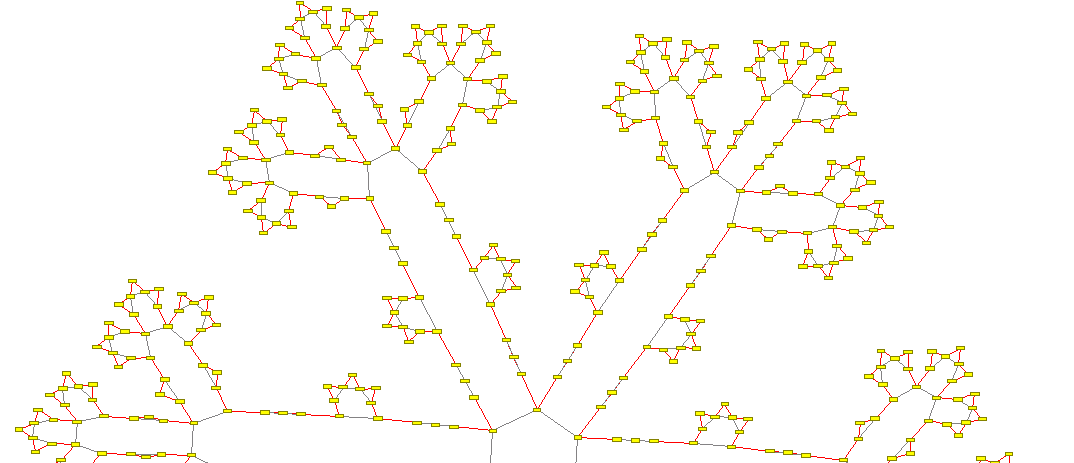
\includegraphics[width=0.9\linewidth]{fig/title}\\[6ex]
  \LARGE Jakob Blomer \qquad Rubino Gei\ss\\ \qquad Edgar Jakumeit\\[3ex]
  \large \today\\

%  \vfill
%	\large Technical Report 2007-5\\
%	\large ISSN 1432-7864

  \setlength{\parindent}{\saveparindent}
\end{titlepage}
\clearpage

\chapter*{Abstract}

\parpic[l] {

\includegraphics[width=45mm]{fig/grgen-256.png}
}

\noindent \textsc{GrGen.NET}: transformation of structures made easy
-- with languages for graph modeling, pattern matching, and rewriting, as well as rule control;
brought to life by a compiler and a rapid prototyping environment offering graphical and step-wise debugging.
The Graph Rewrite Generator is a tool enabling elegant and convenient development of graph rewriting applications with comparable performance to conventionally developed ones.
This user manual contains both, normative statements in the sense of a reference manual as well as an informal guide to the features and usage of \GrG.\\[6ex]

\vspace{13cm}

\parpic[l] {

\includegraphics{fig/by-sa.png}
}
\noindent This manual is licensed under the terms of the \emph{Creative Commons Attribution-Share Alike 3.0 Germany}
license.  The license is available at
\url{http://creativecommons.org/licenses/by-sa/3.0/de/}

\chapter*{Foreword for Release 1.4}
First of all a word about the term ``graph rewriting''.
Some would rather say ``graph transformation''; some even think there is a difference between these two.
We don't see such differences and use graph rewriting for consistency.

The \textsc{GrGen} project started in spring 2003 with the diploma thesis of Sebastian Hack under supervision of Rubino Gei\ss.
At that time we needed a tool to find patterns in graph based intermediate representations used in compiler construction.
We imagined a tool that is fast, expressive, and easy to integrate into our compiler infrastructure.
So far Optimix\cite{assmann00graph} was the only tool that brought together the areas of compiler construction and graph rewriting.
However its approach is to feature many provable properties of the system per se, such as termination, confluence of derivations, and complete coverage of graphs.
This is achieved by restricting the expressiveness of the whole formalism below Turing-completeness.
Our tool \textsc{GrGen} in contrast should be Turing-complete.
Thus \GrG\ provides the user with strong expressiveness but leaves the task of proving such properties to the user.

To get a prototype quickly, we delegated the costly task of subgraph matching to a relational database system~\cite{Hac:03}.
Albeit the performance of this implementation could be improved substantially over the years, we believed that there was more to come.
Inspired by the PhD thesis of Heiko D\"orr~\cite{doerr} we reimplemented our tool to use search plan driven graph pattern matching of its own.
This matching algorithm evolved over time~\cite{adam,Bat:05:SA,Bat:05:DA,Bat:06,BKG:07} and has been ported from C to C\#~\cite{KG:07,Kro:07}. 
In the year 2005 Varr\'o~\cite{gramot2005_adapt} independently proposed a similar search plan based approach.

Though we started four years ago to facilitate some compiler construction problems, in the meantime \GrG\ has grown into a general purpose tool for graph rewriting.\\[3ex]

We want to thank all co-workers and students that helped during the design and implementation of \GrG\ as well as the writing of this manual.
Especially we want to thank Dr.~Sebastian Hack, G.~Veit Batz, Michael Beck, Tom Gelhausen, Moritz Kroll, Dr.~Andreas Ludwig, and Dr.~Markus Noga.
Finally, all this would not happened without the productive atmosphere and the generous support that Prof.~Goos provides at his chair.\\[3ex]

We wish all readers of the manual---and especially all users of \GrG---a pleasant graph rewrite experience.
We hope you enjoy using \GrG\ as much as we enjoy developing it.\\[3ex]

Thank you for using \GrG.\\[6ex]

\noindent Karlsruhe in July 2007, Rubino Gei\ss~on behalf of the \GrG-Team

\pagebreak

\chapter*{Foreword}

Since the last version of this manual which was written for \GrG\ v1.4 a lot has happened, 
as can be seen quite easily in the fact that this manual describes \GrG\ v2.6.
The porting of C to C\# \cite{Kro:07} allowed for a faster pace of development,
which yielded alternatives and subpatterns allowing for structural recursion \cite{Jak:08,StructuralRecursion},
undirected edge support plus fine grain pattern conditions \cite{SABuchwald:2008}, 
a data model that is more user friendly at the API, support for visited flags, 
and an prototypical implementation of an embedding of \GrG\ as a domain specific language into C\# \cite{DAMoritz}
-- resulting in \GrG\ v2.0.
\medskip

Then Dr. Rubino Gei\ss~finished his dissertation \cite{DissRuby} and left; Prof.\ Goos retired.
The succeeding Professor had no commitment to graph rewriting,
so \GrG\ switched from a university project developed by students in their bachelor/masters thesis's
to an open source project (which is still hosted at the IPD, reachable from \url{www.grgen.net}).
\medskip

But development continued:
With the introduction of generic set and map types in the model language to facilitate uses in computer linguistics
and in the rule control language to allow for more concise rule combinations.
With the 2+n pushdown automaton for matching patterns with structural recursion extended 
to handle pattern cardinality specifications and positive applications conditions \cite{ExpressiveConvenientFast:2010}.
With massive API improvements, now featuring an interface of typed, named entities in addition to the old name string and object based interface.
With the introduction of importers and exporters for GXL (the quasi standard graph exchange format in graph rewriting --- but only in theory),
and for GRS, a much easier and less chatty format.\smallskip

Most of these features were introduced due to feedback from users and use cases:\\
We want to thank the organizers of GraBaTs\cite{grabats}, the annual meeting of the graph rewrite tool community,
which gave us the possibility to ruthlessly steal the best ideas of the competing tools.
Thanks to Berthold Hoffmann, for his ``french''-courses and the ideas about how to handle program graphs.
And thanks to several early users giving valuable feedback or even code (\emph{code is of course the best contribution you can give to an open source project}), by name: 
Tom Gelhausen and Bugra Derre (you may have a look at \url{https://svn.ipd.uni-karlsruhe.de/trac/mx/wiki/Home} for their work at the other IPD), Paul Bedaride, Normen Müller, Pieter van Gorp and Nicholas Tung.
\\[1ex]

\noindent Regarding questions please contact the \GrG-Team 
via email to \texttt{grgen} at the host given by \texttt{ipd.info.uni-karlsruhe.de}.\\[1ex]

\noindent We hope you enjoy using \GrG\ even more than we enjoyed developing it\\ {\small(it was fun but aging projects with code traces from many people are not always nice to work with ;).}
\\[1ex]

Thank you for using \GrG.\\[2ex]

\noindent Karlsruhe in November 2010, Edgar Jakumeit on behalf of the \GrG-Team


\clearpage

\tableofcontents

\chapter{Introduction}
\pagenumbering{arabic}


\section{What is \GrG?}

{\scshape GrGen} (\textsc{G}raph \textsc{R}ewrite \textsc{Gen}erator) is a generative programming system for graph rewriting.
For the potentially expensive matching problem, {\scshape GrGen} applies several novel heuristic optimizations.
According to \indexed{Varr\'o's benchmark} it is at least one order of magnitude faster than any other tool known to us.

In order to accelerate the matching step, we internally introduce \newterm{search plans} to represent different \newterm{matching strategies} and equip these search plans with a cost model, taking the present host graph into account.
The task of selecting a good search plan is then considered as an optimization problem~\cite{BKG:07,Bat:06}.
For the rewrite step, our tool implements the well-founded \newterm{single-pushout approach} (SPO, for explanation see \cite{spoapproach}).

For ease of use, {\scshape GrGen} features an expressive specification language and generates program code with a convenient interface.
In contrast to systems like \indexed{Fujaba} \cite{fujaba} our pattern matching algorithm is fully automatic and does not need to be tuned or partly be implemented by hand.
\GrG~\cite{grgen_web} is the successor of the \textsc{GrGen} tool presented at ICGT 2006~\cite{GBGHS:06}. 
The ``.NET'' postfix of the new name indicates that \textsc{GrGen} has been reimplemented in C\# for the Microsoft .NET or Mono environment~\cite{NET,MONO}.


\section{Features of \GrG}

The process of graph rewriting can be divided into four steps:
Representing a graph according to a model, searching a pattern aka finding a match, performing changes to the matched spot in the host graph, and, finally, selecting the next rule(s) for application.
We have organized the features of \GrG\ according to this breakdown of graph rewriting.

\begin{itemize}
  \item The graph model (meta-model) supports:
  \begin{itemize}
    \item Directed graphs
    \item Typed nodes and edges, with multiple inheritance on types
    \item Node and edge types can be equipped with typed attributes (like structs)
    \item Multigraphs (including multiple edges of the same type)
    \item Connection assertions to restrict the ``shape'' of graphs
  \end{itemize}
  
  \item The pattern language supports:
  \begin{itemize}
    \item Plain isomorphic subgraph matching (injective mapping)
    \item Homomorphic matching for a selectable set of nodes/edges, so that the matching is not injective
    \item Attribute conditions (including arithmetic operations on the attributes)
    \item Type conditions (including powerful instanceof-like type expressions)
    \item Parameter passing to rules
    \item \indexed{Dynamic patterns} with iterative or recursive paths and graphs (yet to be implemented)
  \end{itemize}
  
  \item The rewrite language supports:
  \begin{itemize}
    \item Attribute re-calculation (using arithmetic operations on the attributes)
    \item Retyping of nodes/edges (a stronger version of casts of common programming languages)
    \item Creation of new nodes/edges of statically as well as dynamically computed types (some kind of generic templates)
    \item Two modes of specification: A rule can either express changes to be made to the match or replace the whole match (the semantics is always mapped to SPO)
    \item Returning certain edges/nodes for further computations
	  \item Copying (duplicating) of elements form the match---comparable with \indexed{sesqui-pushout} rewriting~\cite{CHHK:06} (yet to be implemented)
  \end{itemize}
  
  \item The rule application language (\GrShell) supports:
  \begin{itemize}
    \item Composing several rules with logical and iterative sequence control (called graph rewrite sequences, GRS)
    \item Various methods for creation/deletion/input/output of graphs/nodes/edges 
    \item Stepwise and graphic debugging of rule application
    \item Graph rewrite sequences that can contain nested transactions\index{transaction, nested} (yet to be implemented)
  \end{itemize}
  
  \item Alternatively to \GrShell, you can access the match and rewrite facility through \LibGr. In this way you can build your own algorithmic rule applications in a .NET language of your choice. 
\end{itemize}


\section{System Overview}

Figure \ref{figsys} gives an overview of the \GrG\ system components. Table \ref{dirstruc} shows the \GrG\ directory structure.

\begin{figure}[htbp]
  \centering
	\scalebox{0.8}{
  \begin{tikzpicture}
      \begin{scope}[shape=rectangle,minimum size=0.75cm,text width=3cm,text centered]
          \tikzstyle{every node}=[draw]
          \node (spec1)    at (0   ,0)    {Rewrite Rules\indexmain{rewrite rule} (*\indexed{.grg})};
          \node (spec2)    at (0   ,2)    {Graph Model\indexmain{graph model} (*\indexed{.gm})};
          \node (grgen)    at (4   ,1)    {\GrG\ Generator\indexmain{generator} (Java, C\#)};
          \node (rewriter) at (10  ,0)    {Rewrite~Rules (C\#)};
          \node (types)    at (10  ,2)    {Graph~Model (C\#)};
          \node (data)     at (14  ,1)    {Graph~Management (C\#)};
          \node (libgr)    at (12  ,4)    {\LibGr\indexmain{libGr}\ (C\#)};
          \node[fill,color=gray] (app)      at (14.1  ,5.6)  {};
          \node[fill=white] (app)      at (14  ,5.5)  {Applications};
          \node (grsh)     at (10  ,5.5)  {\GrShell\indexmain{GrShell}\ (C\#)};
          \node (grs)      at (6   ,5.5)  {Graph Rewrite Script\indexmain{graph rewrite script}\indexmainsee{GrShell script}{graph rewrite script}\indexmainsee{script}{graph rewrite script} (*\indexed{.grs})};
      \end{scope}

      \node[draw, minimum width=9cm,minimum height=4cm] (engine) at (12,1) {};
      \node[draw, minimum width=9cm,minimum height=4cm,style=dotted] (ct) at (2,1) {};
      \node[anchor=north east] (engine_lab) at (engine.north east) {Backend\indexmain{backend} (Run Time)};
      \node[anchor=north east] (ct_lab) at (ct.north east) {Frontend (Compile Time)};

      \draw[->,dashed,red,>=triangle 45]     (spec1)   -> (grgen);
      \draw[->,dashed,red,>=triangle 45]     (spec2)   -> (grgen);
      \draw[->,dashed,red,>=triangle 45]     (grgen)   -> (types);
      \draw[->,line width=1pt,>=triangle 45] (grgen)   -> (engine);
      \draw[->,dashed,red,>=triangle 45]     (grgen)   -> (rewriter);
      \draw[->,line width=1pt,>=triangle 45] (app)     -> (libgr);
      \draw[->,line width=1pt,>=triangle 45] (grsh)    -> (libgr);
      \draw[->,dashed,red,>=triangle 45]     (grs)     -> (grsh);
      \draw[->,line width=1pt,>=triangle 45] (libgr)   -> (engine);

      \draw[->,line width=1pt,>=triangle 45] (-1.25,5.5) -- +(2.5,0) node[above, midway] {call};
      \draw[->,dashed,red,>=triangle 45] (-1.25,4.5)  -- +(2.5,0) node[above, midway] {read / generate};
  \end{tikzpicture}
	}
  \caption{\GrG\ system components \cite{Kro:07}}
  \label{figsys}
\end{figure}
\begin{table}[htbp]
  \begin{tabularx}{\linewidth}{|lX|} \hline
  bin & Contains the .NET assemblies, in particular \indexed{GrGen.exe} (the graph rewrite system generator), \indexed{LGSPBackend.dll} (a \GrG\ backend), \indexed{LibGr.dll} (the backend API), and the shell \indexed{GrShell.exe}.  \\ 
  lib & Contains the \GrG\ generated assemblies (*.dll). \\
  specs & Contains the graph rewrite system source documents (*.gm and *.grg). \\ \hline
  \end{tabularx}
  \caption{\GrG\ directory structure}
  \label{dirstruc}
\end{table}

A graph rewrite system\footnote{In this context, system is not a CH0-like grammar rewrite system, but rather a set of interacting software components.} is defined by a rule set file (*.grg) and zero or more graph model description files (*.gm). 
Such a graph rewrite system is generated from these specifications by GrGen.exe and can be used by applications such as \GrShell.
Figure \ref{process} shows the generation process.

\begin{figure}[htbp]
  \centering
	\scalebox{0.8}{
  \begin{tikzpicture}
      \begin{scope}[shape=rectangle,minimum size=0.75cm,text width=3cm,text centered]
          \tikzstyle{every node}=[draw]
          \node (gm1)      at (0   ,0)    {model1.gm};
          \node (gm2)      at (0   ,1)    {model2.gm};
          \node (gm3)      at (0   ,2)    {model3.gm};
          \node (grg)      at (4.5 ,1)    {rules1.grg};
          \node (grgen)    at (10   ,1)    {GrGen.exe};
          \node (act)      at (15.5,1) {rules1Actions.dll};
          \node (backend)  at (10   ,2)    {backend.dll};
          \node (mod)      at (15.5,2)  {rules1Model.dll};
      \end{scope}
         
			\draw[|-|] (-1,-1.5)   -- (5.5, -1.5)    node[below, midway] {/specs};
			\draw[|-|] (9,-1.5)    -- (11, -1.5)     node[below, midway] {/bin};
			\draw[|-|] (14.5,-1.5) -- (16.5, -1.5)   node[below, midway] {/lib};

      \draw[->,line width=1pt,>=triangle 45]     (grg)     -> (gm1);
      \draw[->,line width=1pt,>=triangle 45]     (grg)     -> (gm2);
      \draw[->,line width=1pt,>=triangle 45]     (grg)     -> (gm3);
      \draw[->,dashed,red,>=triangle 45]         (grg)     -> (grgen);
      \draw[->,dashed,red,>=triangle 45]         (grgen)   -> (mod);
      \draw[->,dashed,red,>=triangle 45]         (grgen)   -> (act);
      \draw[->,line width=1pt,>=triangle 45]     (mod)     -> (backend);
      \draw[->,line width=1pt,>=triangle 45]     (act)     -> (backend);


      \draw[->,line width=1pt,>=triangle 45] (-1.25,3.0) -- +(2.5,0) node[above, midway] {referencing};
      \draw[->,dashed,red,>=triangle 45]     (3.25,3.0)  -- +(2.5,0) node[above, midway] {read / generate};
  \end{tikzpicture}
	}
  \caption{Generating a graph rewrite system}
  \label{process}
\end{figure}

In general you have to distinguish carefully between a graph model (meta level), a host graph, a pattern graph and a rewrite rule.
In \GrG\ pattern graphs are implicitly defined by rules, i.e.\ each rule defines its pattern.
On the technical side, specification documents for a graph rewrite system can be available as source documents for graph models and rule sets (plain text *.gm and *.grg files) or as their translated .NET modules, either C\# source files or their compiled assemblies (*.dll).

Generating a \GrG\ graph rewrite system may be considered as preliminary task.
The actual process of rewriting as well as dealing with host graphs is performed by \GrG's backend.
\GrG\ provides a backend \indexed{API}---the .NET library \LibGr.
For most issues---in particular for experimental purposes---you might rather want to work with the \GrShell\ because of its more convenient interface.
However, \GrShell\ does not provide the full power of the \LibGr; see also note \ref{note:indeterminism} on page \pageref{note:indeterminism}.

\section{What is Graph Rewriting?}
\label{ov:whatsallabout}

The notion of graph rewriting as understood by \GrG\ is a method for declaratively specifying ``changes'' to a graph.
This is comparable to the well-known term rewriting. 
Normally you use one or more \newterm{graph rewrite rules} to accomplish a certain task.
\GrG\ implements an SPO-based approach.
In the simplest case such a graph rewrite rule consists of a tuple $L \rightarrow R$, whereas $L$---the \newterm{left hand side}\indexmainsee{LHS}{left hand side} of the rule---is called \newterm{pattern graph} and $R$---the \newterm{right hand side}\indexmainsee{RHS}{right hand side} of the rule---is the \newterm{replacement graph}.

\begin{figure}[htbp]
	\centering
  \begin{tikzpicture}
    \begin{scope}[minimum size=0.5cm]
      \tikzstyle{every node}=[draw]
      \node (L)     at (0   ,2.5) {$L$};
      \node (R)     at (7   ,2.5) {$R$};
      \node (mL)    at (0   ,0) {};
      \node (mR)    at (7   ,0) {};
      \node[text width=2cm,text badly ragged,minimum size=1cm] (H)     at (0   ,0) {$H$};
      \node[text width=2cm,text badly ragged,minimum size=1cm] (Hs)    at (7   ,0) {$H'$};
    \end{scope}

    \draw[dotted,->] (L) node[above=0.4cm] {Pattern Graph} -> (mL) node[left,midway]  {Match $m$}   node[below=0.6cm] {Host Graph};
    \draw[dotted,->] (R) node[above=0.4cm] {Rewrite Graph} -> (mR)                              node[below=0.6cm] {Result Graph};

    \pgfsetshortenstart{0.5cm}
    \pgfsetshortenend{0.5cm}
    \draw[thick,->]  (L) -> (R)  node[above,midway] {Preservation Morphism $r$} node[below,midway] {Rule};
    \draw[thick,->]  (H) -> (Hs) node[below,midway] {Rule Application};
  \end{tikzpicture}
  \caption{Basic Idea of Graph Rewriting}
  \label{figrule}
\end{figure}

Moreover we need to identify graph elements (nodes or edges) of $L$ and $R$ for preserving them during rewrite. 
This is done by a \newterm{preservation morphism} $r$ mapping elements from $L$ to $R$; the morphism $r$ is injective, but needs to be neither surjective nor total.
Together with a rule name $p$ we have $p : L \xrightarrow{r} R$.

The transformation is done by \newterm{application}\indexmainsee{rule application}{application} of a rule to a \newterm{host graph} $H$.
To do so, we have to find an occurrence of the pattern graph in the host graph. 
Mathematically speaking, such a \newterm{match} $m$ is an isomorphism from $L$ to a subgraph of $H$.
This morphism may not be unique, i.e.\ there may be several matches.
Afterwards we change the matched \indexed{spot} $m(L)$ of the host graph, such that it becomes an isomorphic subgraph of the replacement graph $R$.
Elements of $L$ not mapped by $r$ are deleted from $m(L)$ during rewrite.
Elements of $R$ not in the image of $r$ are inserted into $H$, all others (elements that are mapped by $r$) are retained.
The outcome of these steps is the resulting graph $H'$. In symbolic language: $H \xRightarrow{m, p} H'$.


\section{An Example}
\label{ov:example}

We'll have a look at a small example. 
We start using a special case to construct our host graph: an \indexed{empty pattern} always produces exactly one\footnote{Because of the uniqueness of the total and totally undefined morphism.} match (independent of the host graph). So we construct an apple by applying
\[
  p_0:  
  \begin{array}[c]{c} 
    \emptyset
  \end{array} 
  \begin{array}[c]{c} 
    \longrightarrow 
  \end{array} 
  \begin{array}[c]{c} 
    \begin{tikzpicture}[show background rectangle]
      \tikzstyle{every node}=[circle]
      \node[draw] (n1) at (2.5,5) {};
      \node[draw] (n2) at (2,4)   {};
      \node[draw] (n3) at (0,2)   {};
      \node[draw] (n4) at (2,0)   {};
      \node[draw] (n5) at (4,2)   {};
    	
    	\draw[-latex] (n2) --                                  (n1) node[left,midway]  {$e_1$};
    	\draw[-latex] (n2) .. controls +(-1,1) and +(0,1) ..   (n3) node[left,midway]  {$e_2$};
      \draw[-latex] (n3) .. controls +(0,-1) and +(-1,0) ..  (n4) node[left,midway]  {$e_3$};
    	\draw[-latex] (n4) .. controls +(1,0)  and +(0,-1) ..  (n5) node[right,midway] {$e_4$};
      \draw[-latex] (n5) .. controls +(0,1)  and +(1,1) ..   (n2) node[right,midway] {$e_5$};
    \end{tikzpicture}
  \end{array}
\]
to the empty host graph. 
As the result we get an apple as new host graph $H$. 
Now we want to rewrite our apple with stem to an apple with a leaflet. 
So we apply
\[
  p_1:
  \begin{array}[c]{c}
    \begin{tikzpicture}[show background rectangle]
      \tikzstyle{every node}=[circle,minimum size=0.7cm]
      \node[draw] (a) at (2,5.5)  {a};
      \node[draw] (b) at (2,4)    {b};
    	
    	\draw[-latex] (b) -- (a) node[left,midway]  {$x$};
    \end{tikzpicture}
  \end{array}
  \begin{array}[c]{c}
    \longrightarrow
  \end{array}
  \begin{array}[c]{c}
    \begin{tikzpicture}[show background rectangle]
      \tikzstyle{every node}=[circle,minimum size=0.7cm]
      \node[draw] (c) at (2,5.5)  {c};
      \node[draw] (b) at (2,4)    {b};
    	
    	\draw[-latex] (b) .. controls +(-0.7,+0.7) and +(-0.7,-0.7) .. (c) node[left,midway]   {$y$};
    	\draw[-latex] (b) .. controls +(+0.7,+0.7) and +(+0.7,-0.7) .. (c) node[right,midway]  {$z$};
    \end{tikzpicture}
  \end{array} 
\]
to $H$ and get the new host graph $H_1$, something like this:
\[
  \begin{array}[c]{c} 
    \begin{tikzpicture}[show background rectangle]
      \tikzstyle{every node}=[circle]
      \node[draw] (n1) at (2.5,5) {};
      \node[draw] (n2) at (2,4)   {};
      \node[draw] (n3) at (0,2)   {};
      \node[draw] (n4) at (2,0)   {};
      \node[draw] (n5) at (4,2)   {};
    	
    	\draw[-latex] (n2) --                                  (n1) node[left,midway]  {$e_1$};
    	\draw[-latex] (n2) .. controls +(-1,1) and +(0,1) ..   (n3) node[left,midway]  {$e_2$};
      \draw[-latex] (n3) .. controls +(0,-1) and +(-1,0) ..  (n4) node[left,midway]  {$e_3$};
    	\draw[-latex] (n4) .. controls +(1,0)  and +(0,-1) ..  (n5) node[right,midway] {$e_4$};
      \draw[-latex] (n5) .. controls +(0,1)  and +(1,1) ..   (n2) node[right,midway] {$e_5$};
    \end{tikzpicture}
  \end{array} 
  \begin{array}[c]{c} 
    \xRightarrow{\quad p_1 \quad}
  \end{array} 
  \begin{array}[c]{c} 
    \begin{tikzpicture}[show background rectangle]
      \tikzstyle{every node}=[circle]
      \node[draw] (n1) at (2.5,5) {};
      \node[draw] (n2) at (2,4)   {};
      \node[draw] (n3) at (0,2)   {};
      \node[draw] (n4) at (2,0)   {};
      \node[draw] (n5) at (4,2)   {};
      \node[draw] (n6) at (0,0.5)   {};
    	
    	\draw[-latex] (n2) --                                  (n1) node[left,midway]  {$e_1$};
    	\draw[-latex] (n2) .. controls +(-1,1) and +(0,1) ..   (n3) node[left,midway]  {$e_2$};
      \draw[-latex] (n3) .. controls +(-0.7,-0.7) and +(-0.7,+0.7) .. (n6) node[left,midway]  {$e_6$};
      \draw[-latex] (n3) .. controls +(+0.7,-0.7) and +(+0.7,+0.7) .. (n6) node[right,midway] {$e_7$};
    	\draw[-latex] (n4) .. controls +(1,0)  and +(0,-1) ..  (n5) node[right,midway] {$e_4$};
      \draw[-latex] (n5) .. controls +(0,1)  and +(1,1) ..   (n2) node[right,midway] {$e_5$};
    \end{tikzpicture}
  \end{array}
\]
What happened? 
\GrG\ has arbitrarily chosen one match out of the set of possible matches, because $x$ matches edge $e_3$ as well as $e_1$.
A correct solution could make use of edge type information. 
We have to change rule $p_0$ to generate the edge $e_1$ with a special type ``stem''.
And this time we'll even keep the stem. 
So let
\[
  p_2:
  \begin{array}[c]{c}
    \begin{tikzpicture}[show background rectangle]
      \tikzstyle{every node}=[circle,minimum size=0.7cm]
      \node[draw] (a) at (2,5.5)  {a};
      \node[draw] (b) at (2,4)    {b};
    	
    	\draw[-latex] (b) -- (a) node[left,midway]  {$x:\text{stem}$};
    \end{tikzpicture}
  \end{array}
  \begin{array}[c]{c}
    \longrightarrow
  \end{array}
  \begin{array}[c]{c}
    \begin{tikzpicture}[show background rectangle]
      \tikzstyle{every node}=[circle,minimum size=0.7cm]
      \node[draw] (c) at (2,5.5)  {c};
      \node[draw] (b) at (2,4)    {b};
      \node[draw] (a) at (3.5,5.5){a};
    	
    	\draw[-latex] (b) -- (a) node[right,midway]  {$x$};
    	\draw[-latex] (b) .. controls +(-0.7,+0.7) and +(-0.7,-0.7) .. (c) node[left,midway]   {$y$};
    	\draw[-latex] (b) .. controls +(+0.7,+0.7) and +(+0.7,-0.7) .. (c) node[above,midway]  {$z$};
    \end{tikzpicture}
  \end{array}.
\]
If we apply $p_2$ to the modified $H_1$ this leads to
\[
  \begin{array}[c]{c} 
    \begin{tikzpicture}[show background rectangle]
      \tikzstyle{every node}=[circle]
      \node[draw] (n1) at (2.5,5) {};
      \node[draw] (n2) at (2,4)   {};
      \node[draw] (n3) at (0,2)   {};
      \node[draw] (n4) at (2,0)   {};
      \node[draw] (n5) at (4,2)   {};
    	
    	\draw[-latex] (n2) --                                  (n1) node[left,pos=0.8]  {$e_1:\text{stem}$};
    	\draw[-latex] (n2) .. controls +(-1,1) and +(0,1) ..   (n3) node[left,midway]  {$e_2$};
      \draw[-latex] (n3) .. controls +(0,-1) and +(-1,0) ..  (n4) node[left,midway]  {$e_3$};
    	\draw[-latex] (n4) .. controls +(1,0)  and +(0,-1) ..  (n5) node[right,midway] {$e_4$};
      \draw[-latex] (n5) .. controls +(0,1)  and +(1,1) ..   (n2) node[right,midway] {$e_5$};
    \end{tikzpicture}
  \end{array} 
  \begin{array}[c]{c} 
    \xRightarrow{\quad p_2 \quad}
  \end{array} 
  \begin{array}[c]{c} 
    \begin{tikzpicture}[show background rectangle]
      \tikzstyle{every node}=[circle]
      \node[draw] (n1) at (3,5) {};
      \node[draw] (n2) at (2,4)   {};
      \node[draw] (n3) at (0,2)   {};
      \node[draw] (n4) at (2,0)   {};
      \node[draw] (n5) at (4,2)   {};
      \node[draw] (n6) at (2,5.0)   {};
    	
    	\draw[-latex] (n2) --                                  (n1) node[right,pos=0.6] {$e_1:\text{stem}$};
    	\draw[-latex] (n2) .. controls +(-1,1) and +(0,1) ..   (n3) node[left,midway]  {$e_2$};
      \draw[-latex] (n3) .. controls +(0,-1) and +(-1,0) ..  (n4) node[left,midway]  {$e_3$};
    	\draw[-latex] (n4) .. controls +(1,0)  and +(0,-1) ..  (n5) node[right,midway] {$e_4$};
      \draw[-latex] (n5) .. controls +(0,1)  and +(1,1) ..   (n2) node[right,midway] {$e_5$};
    	\draw[-latex] (n2) .. controls +(-0.3,+0.3) and +(-0.3,-0.3) .. (n6) node[left,midway]   {};
    	\draw[-latex] (n2) .. controls +(+0.3,+0.3) and +(+0.3,-0.3) .. (n6) node[right,midway]  {};
    \end{tikzpicture}
  \end{array}.
\]

\section{The Tools}

All the programs and libraries of \GrG\ are licensed under \indexed{LGPL}. Notice that the \yComp\ graph viewer is not a part of \GrG\; \yComp\ ships with its own license.

\subsection{\texttt{\indexed{GrGen.exe}}}
The \texttt{GrGen.exe} assembly implements the \GrG\ generator. The \GrG\ generator parses a rule set and its model files and compiles them into .NET assemblies. The compiled assemblies interact with the \GrG\ backend.
\begin{description}
  \item[Usage] \texttt{[mono] GrGen.exe [-use <existing-dir>] [-d] <rule-set> [<output-dir>]}\\
    \emph{rule-set} is a file containing a rule set specification according to chapter \ref{chaprulelang}. Usually such a file has the suffix \texttt{\indexed{.grg}}. The suffix \texttt{.grg} may be omitted.
By default \GrG\ tries to write the compiled assemblies to the directory \texttt{../lib} relative to the path of \texttt{GrGen.exe}. This can be changed by the optional parameter \emph{output-dir}.
  \item[Options] \mbox{} 
    \begin{tabularx}{\linewidth}{lX}
      \texttt{-d} & Enable debug output. A subdirectory \texttt{tmpgrgen$n$}\footnote{$n$ is an increasing number.} within the current directory will be created. This directory contains:
\begin{itemize}
  \item \texttt{printOutput.txt}---a snapshot of \texttt{stdout} during program execution.
  \item \emph{Name}\texttt{Actions.cs}---the C\# source file of the \emph{rule-set}\texttt{Actions.dll} assembly.
  \item \emph{Name}\texttt{Model.cs}---the C\# source file(s) of the \emph{rule-set}\texttt{Modell.dll} assembly.
\end{itemize}\\
      \texttt{-use} & Don't re-generate C\# source files. Instead use the files in \emph{existing-dir} to build the assemblies.	
    \end{tabularx}
  \item[Requires] .NET 2.0 (or above) or Mono 1.2.2 (or above). Java Runtime Environment 1.5 (or above).
\end{description}

\subsection{\texttt{\indexed{GrShell.exe}}}
The \GrShell\index{GrShell} is a shell application of the \LibGr. \GrShell\ is capable of creating, manipulating, and dumping graphs as well as performing graph rewriting with graphical debug support. For further information about the \GrShell\ language see chapter \ref{chapgrshell}.

\begin{description}
  \item[Usage] \texttt{[mono] grShell.exe [-c "<commands>" | <grshell-script>]}\\
     Opens the interactive shell. The \GrShell\ will execute the commands in \emph{grshell-script}\indexmain{graph rewrite script} (usually a \texttt{*\indexed{.grs}} file) immediately.  
  \item[Options] \mbox{} 
    \begin{tabularx}{\linewidth}{lX}
      \texttt{-c} & Execute the quoted \GrShell\ commands immediately. Instead of a line break use a double semicolon \texttt{;;} as command separation terminal.
    \end{tabularx}
  \item[Requires] .NET 2.0 (or above) or Mono 1.2.2 (or above).
\end{description}

\subsection{\texttt{\indexed{LibGr.dll}}}
The \LibGr\indexmain{libGr} is a .NET assembly implementing \GrG's \indexed{API}. See the extracted HTML documentation for interface descriptions. 

\subsection{\texttt{\indexed{yComp.jar}}}
\label{tools:ycomp}
<<<<<<< .mine
\yComp\index{yComp}\cite[] is a graph visualization tool based on \yFiles\cite[]. It is well integrated in \GrG, but it's not a part of \GrG. \yComp\ implements several graph layout algorithms and has file format support for \indexed{VCG}, GML, and YGF among others. Notice that \yComp\ is not free software. However, it's free for use in academic and non-commercial areas.\\
=======
\yComp\index{yComp}\cite{ycomp} is a graph visualization tool based on \yFiles\cite{yfiles}. It is well integrated in \GrG, but it's not a part of \GrG. \yComp\ implements several graph layout algorithms and has file format support for \indexed{VCG}, GML and YGF among others. Notice that \yComp\ is not free software. However, it's free for use in academic and non-commercial areas.\\
>>>>>>> .r14583

\begin{description}
  \item[Usage] Usually \yComp\ will be loaded by the \GrShell. You might want to open \yComp\ manually by typing\\
   \texttt{java -jar yComp.jar [<graph-file>]}\\
  The \emph{graph-file} may be any graph file in a supported format. \yComp\ will open this file on startup.
<<<<<<< .mine
  \item[Hints] Do not use the \indexedsee{compiler graph}{layout algorithm} \indexed{layout algorithm} (\yComp's default setting). Instead \texttt{\indexedsee{Organic}{layout algorithm}} or \texttt{\indexedsee{Orthogonal}{layout algorithm}} might be good choices. Use the rightmost blue play button to start layouting. This may take a while, depending on the graph size.
=======
  \item[Hints] Do not use the \indexedsee{compiler graph}{layout algorithm} \indexed{layout algorithm} (\yComp's default setting). Instead \texttt{\indexedsee{Organic}{layout algorithm}} or \texttt{\indexedsee{Orthogonal}{layout algorithm}} might be good choices. Use the rightmost blue play button to start layout process. This may take a while, depending on the graph size:
>>>>>>> .r14583
\begin{center}
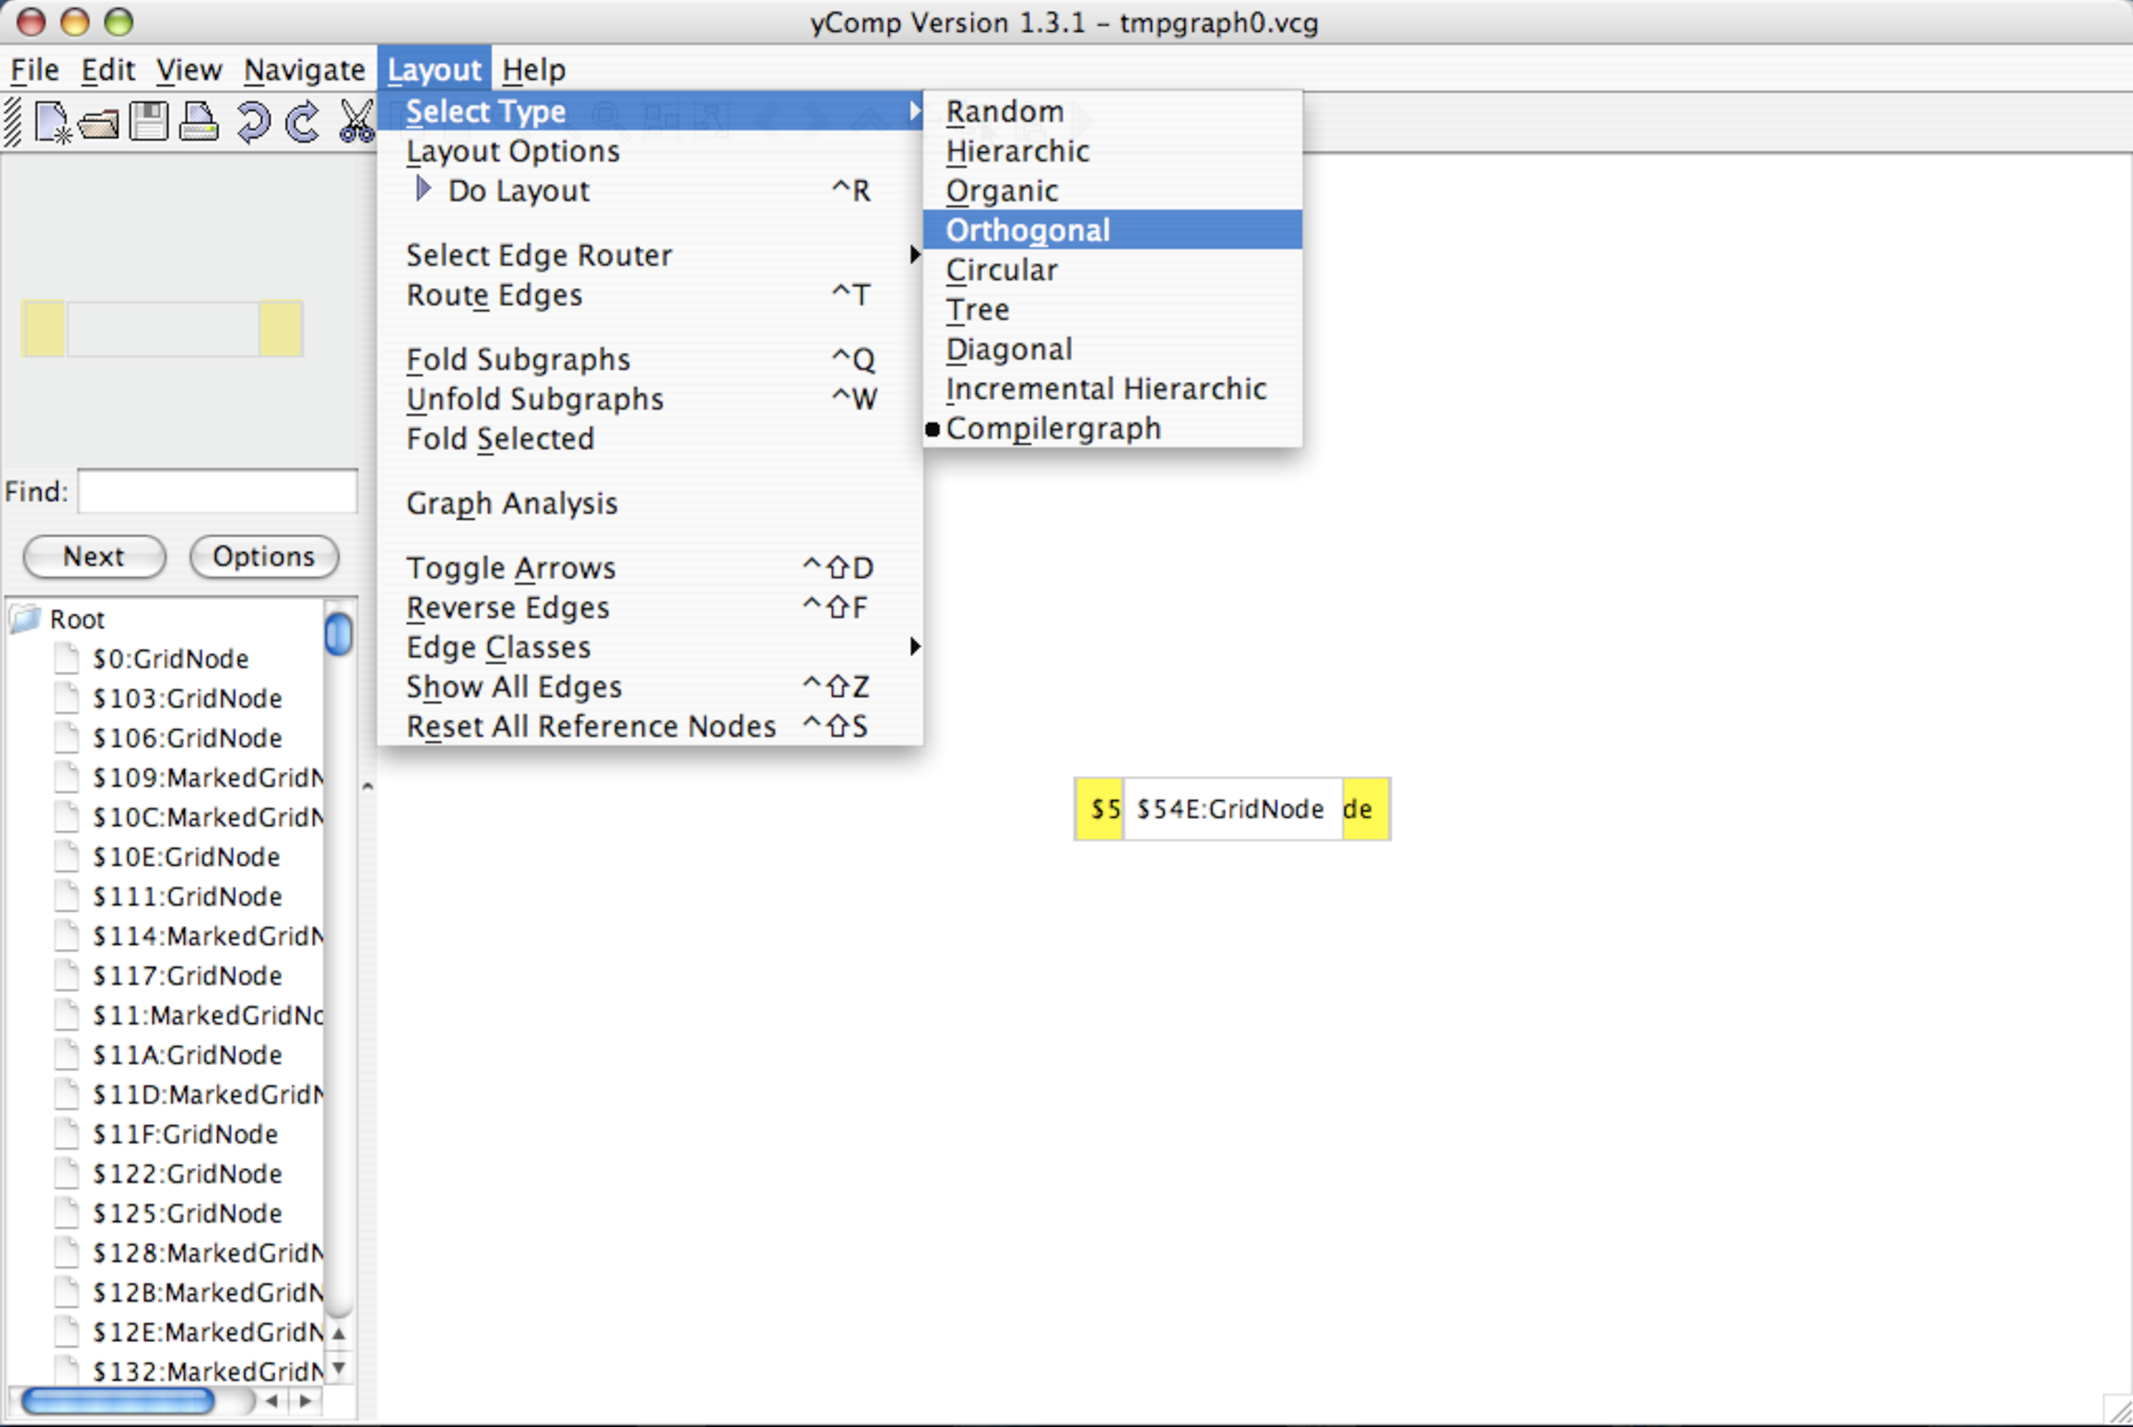
\includegraphics[width=0.45\linewidth]{fig/ycomp1.pdf} 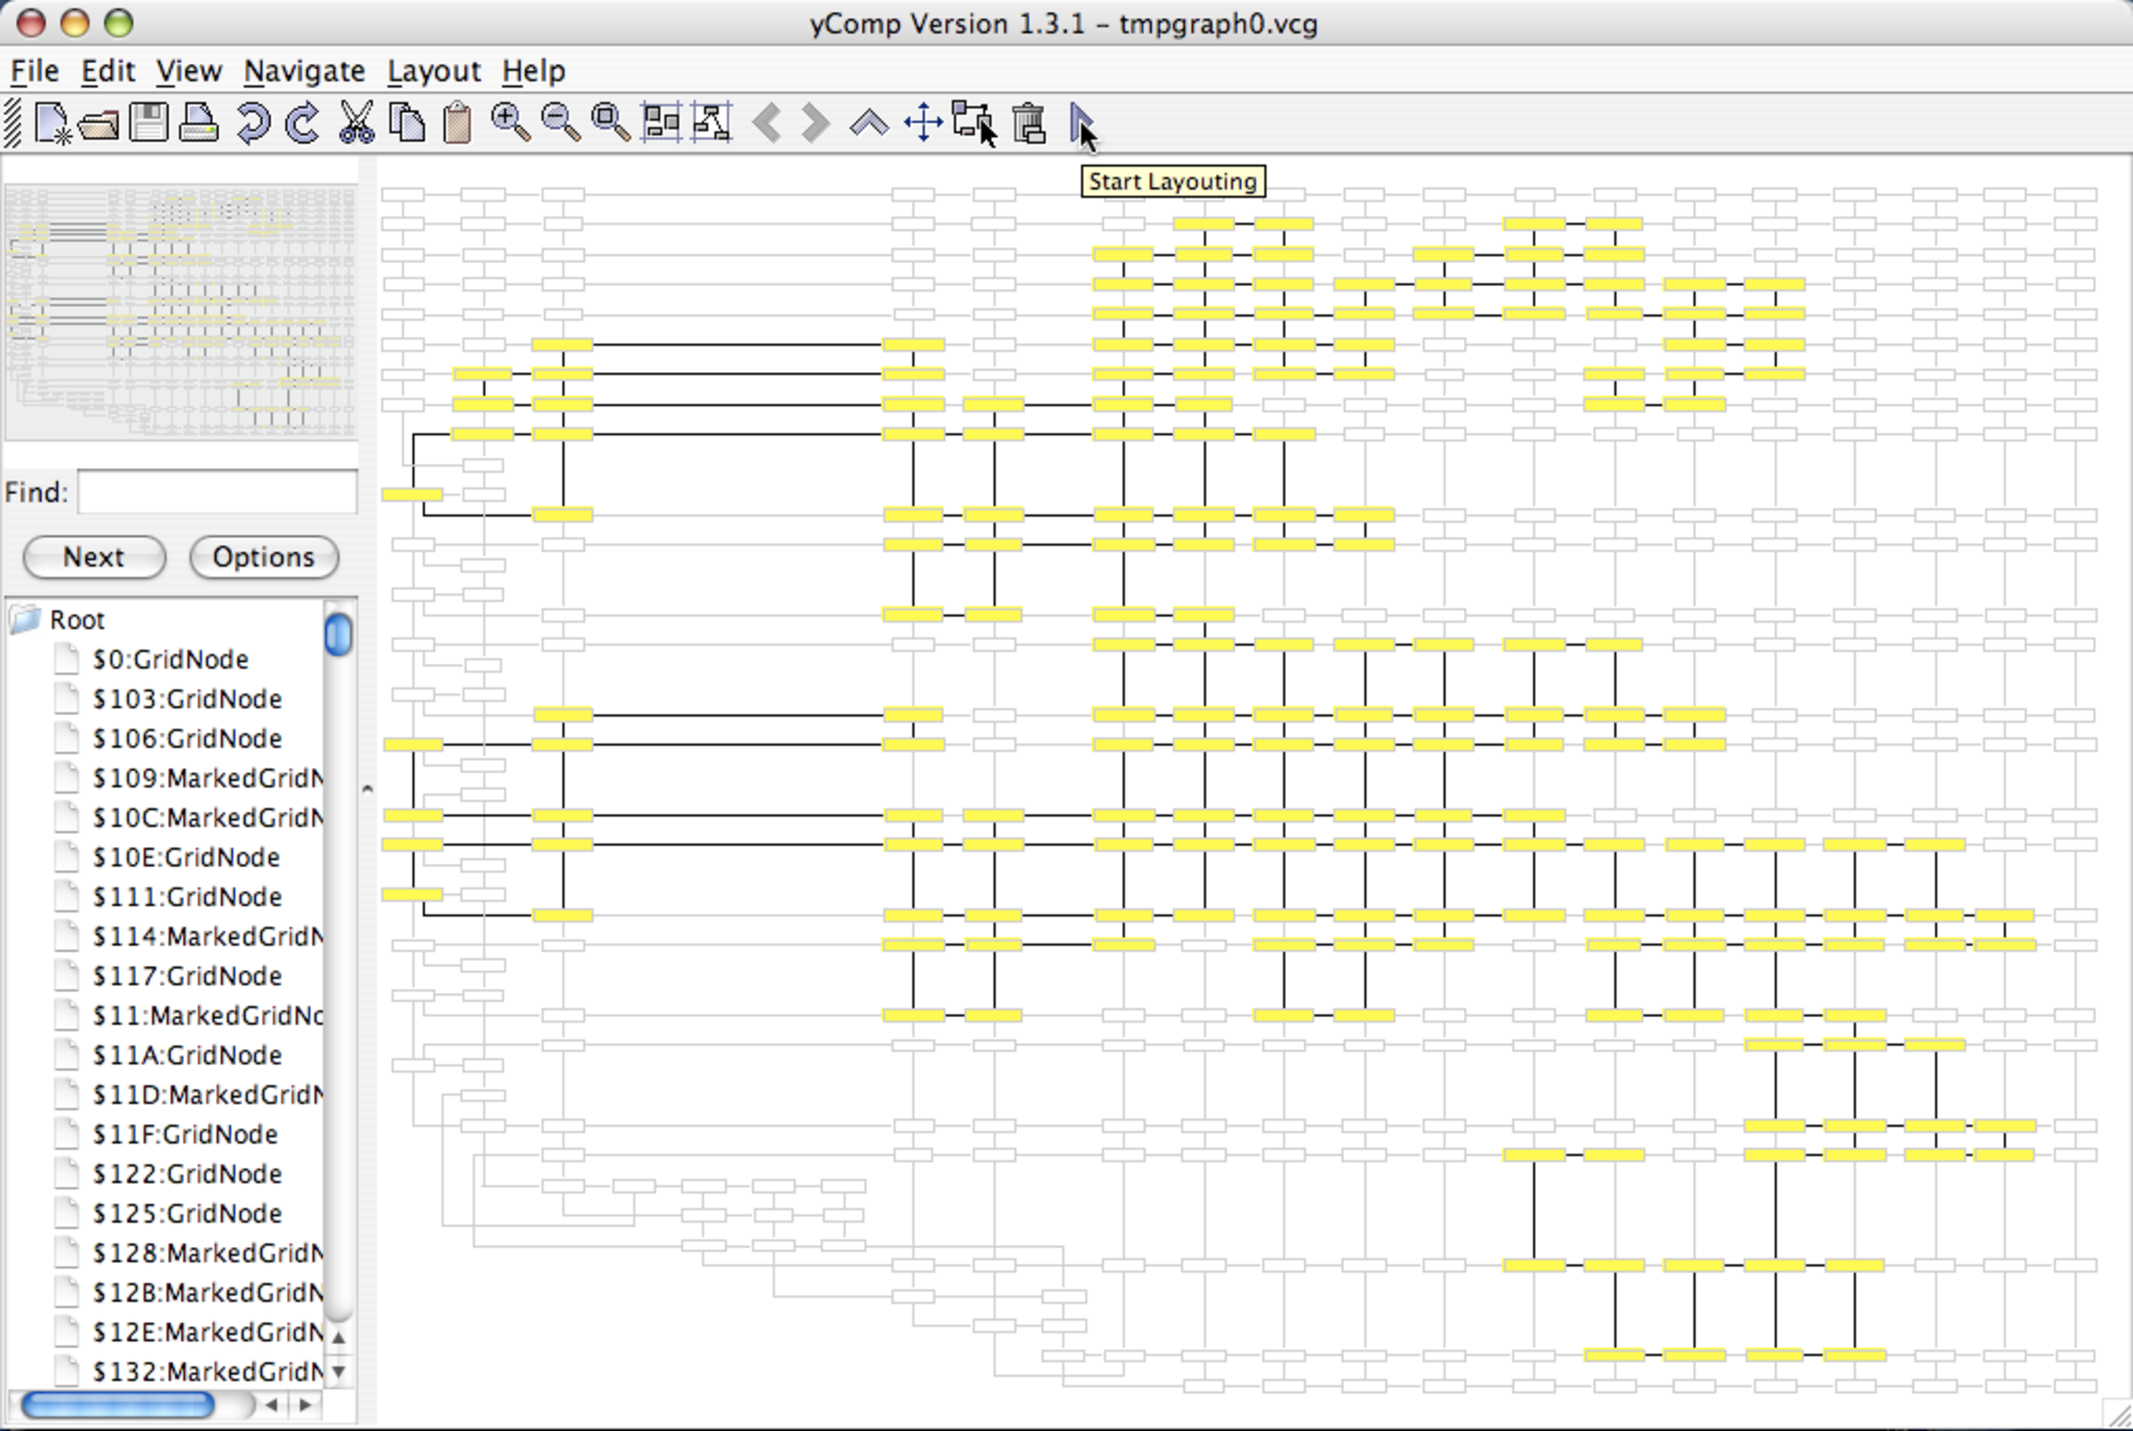
\includegraphics[width=0.45\linewidth]{fig/ycomp2.pdf}
\end{center}
  \item[Requires] Java Runtime Environment 1.5 (or above).
\end{description}




\chapter{Quickstart}\indexmain{quickstart}

In this chapter we'll build a \GrG\ system from scratch. 
You should already have read Chapter~\ref{chp:intro} to have a glimpse of the \GrG\ system and its components.
We will use \GrG\ to construct non-deterministic state machines.
We further show some actual graph rewriting by removing $\varepsilon$-transitions from our state machines.
This chapter is mostly about the \GrG\ look and feel; please take a look at the succeeding chapters for comprehensive specifications.

\section{Downloading \& Installing}
If you are reading this document, you probably did already download the \GrG\ software from our website (\url{http://www.grgen.net}).
Make sure you have the following system requirements installed
\begin{itemize}
	\item Java 1.5 or above \footnotesize{(ensure \texttt{java} is available in the search path)}
	\item Mono 1.2.3 or above on Unix-like platforms / .NET 2.0 or above on Microsoft Windows 
\end{itemize}
Unpack the package to a directory of your choice, for example into \texttt{/opt/grgen} and \texttt{/opt/ycomp}:
\begin{bash}
mkdir /opt/grgen
tar xvfj GrGenNET-V1_3_1-2007-12-06.tar.bz2
mv GrGenNET-V1_3_1-2007-12-06/* /opt/grgen/
rmdir GrGenNET-V1_3_1-2007-12-06
\end{bash}
Add the \texttt{/opt/grgen/bin} directory to your search paths, for instance if you use \texttt{bash} add a line to your \texttt{/home/.profile} file.
\begin{bash}
export PATH=/opt/grgen/bin:$PATH
\end{bash}
Furthermore we create a directory for our \GrG\ data, for instance by \texttt{mkdir /home/grgen}.

\begin{figure}[htbp]
    \begin{note}
        {\bf If you're using Microsoft Windows:}
        On Windows make sure you have the .NET 2.0 (or above) framework installed.
        \GrG\ does not need to be ``installed'', just copy the extracted files to a directory of your choice.
        Add this directory to your search paths via \emph{control panel} $\rightarrow$ \emph{system properties}.
        You might rather want to download the zip archive instead of the bz2 archive.
        Execute the \GrG\ assemblies from a command line window (\emph{Start} $\rightarrow$ \emph{Run...} $\rightarrow$ \texttt{cmd}); On Windows / .NET the \texttt{mono} prefix is not applicable, of course.\\
        If you are using Notepad++ you may be interested in the syntax highlighting for the model and rule language of \GrG\ provided in the syntaxhighlighting directory.
    \end{note}
\end{figure}

\section{Creating a Graph Model}
In the directory \texttt{/home/grgen} we create a text file \texttt{StateMachine.gm} that contains the graph meta model for our state machine\footnote{You'll find the source code of this quick start example shipped with the \GrG\ package in the \texttt{examples/FiniteStateMachine/} directory.}.
By graph meta model we mean a set of node types and edge types which are available for building state machine graphs (see Chapter~\ref{chapmodellang}).
Figure \ref{fig:quick:mm} shows the meta model.
\begin{figure}[htbp]
    \centering
    \begin{grgen}
node class State {
    id: int;
}

abstract node class SpecialState extends State;
node class StartState extends SpecialState;
node class FinalState extends SpecialState;
node class StartFinalState extends StartState, FinalState;

edge class Transition {
    Trigger: string;
}

const edge class EpsilonTransition extends Transition;    
    \end{grgen}
    \caption{Meta Model for State Machines}
    \label{fig:quick:mm}
\end{figure}    
What have we done?
You can see two base types, \texttt{State} for state nodes and \texttt{Transition} for transition edges that will connect the state nodes.
\texttt{State} has an integer attribute \texttt{id} and \texttt{Transition} has a string attribute \texttt{Trigger} which indicates the character sequence for switching from the source state node to the destination state node.
For the rest of the types we use inheritance (keyword \texttt{extends}) which works more or less like inheritance in object oriented languages.
Accordingly the \texttt{abstract} modifier for \texttt{SpecialState} means that you cannot create a node of that precise type, but you might create nodes of non-abstract subtypes.
As you can see \GrG\ supports multiple inheritance, and with \texttt{StartFinalState} we have constructed a ``diamond'' type hierarchy.

\section{Creating Graphs}
\label{sct:quick:create}
Let's test our graph meta model by creating a state machine graph.
We will use the \GrShell\ (see Chapter~\ref{chapgrshell}) and---for visualization---\yComp.
To get everything working we need a rule set file, too.
For the moment we just create an almost empty file \texttt{removeEpsilons.grg} in the \texttt{/home/grgen} directory, containing only the line
\begin{grgen}
using StateMachine;
\end{grgen}
Now, we could start by launching the \GrShell\ and typing the commands interactively.
This is, however, in most of the cases not the preferred way.
We rather create a \GrShell\ script, say \texttt{removeEpsilons.grs}, in the \texttt{/home/grgen} directory.
Figure \ref{fig:quick:shell} shows this script.
Run the script by executing \texttt{grshell removeEpsilons.grs}.
The first time you execute the script, it might take a while because \GrG\ has to compile the meta model and the rule set into .NET assemblies.
\begin{figure}[htbp]
    \centering
    \begin{grgen}
new graph removeEpsilons "StateMachineGraph"

new :StartState($=S, id=0)
new :FinalState($=F, id=3)
new :State($="1", id=1)
new :State($="2", id=2)
new @(S)-:Transition(Trigger="a")-> @("1")
new @("1")-:Transition(Trigger="b")-> @("2")
new @("2")-:Transition(Trigger="c")-> @(F)
new @(S)-:EpsilonTransition-> @("2")
new @("1")-:EpsilonTransition-> @(F)
new @(S)-:EpsilonTransition-> @(F)

show graph ycomp
    \end{grgen}
    \caption{Constructing a state machine graph in \GrShell}
    \label{fig:quick:shell}
\end{figure}
The graph viewer \yComp\ opens and after clicking the blue ``layout graph'' button on the very right side of the button bar, you get a window similiar to figure \ref{fig:quick:ycomp} (see also Section~\ref{tools:ycomp}).
\begin{figure}[htbp]
	\centering
	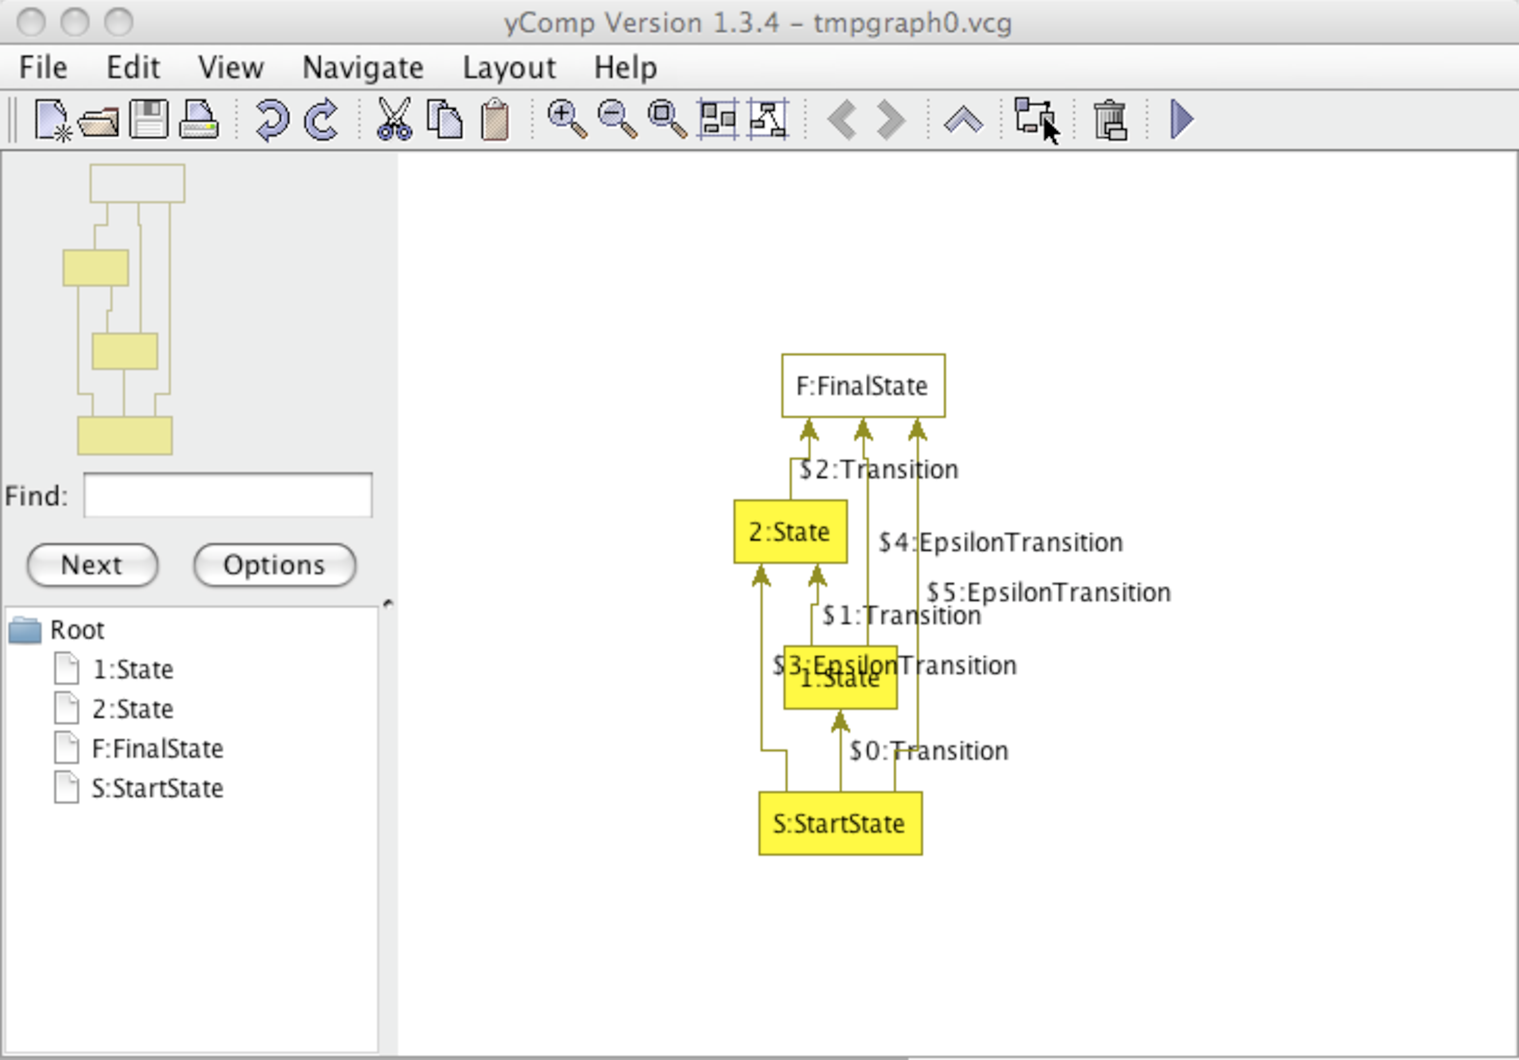
\includegraphics[width=0.8\linewidth]{fig/quickycomp}
	\caption{A first state machine}
	\label{fig:quick:ycomp}
\end{figure}
The graph looks still a bit confusing.
In fact it is quite normal that \yComp's automatic layout algorithm needs manual adjustments.
Quit \yComp\ and exit the \GrShell\ by typing \texttt{exit}.

This script starts with creating an empty graph of the meta model \texttt{StateMachine} (which is referenced by the rule set \texttt{removeEpsilons.grg}) with the name \texttt{StateMachineGraph}.
Thereafter we create nodes and edges.
The colon notation indicates a node or edge type.
Also note the inplace-arrow notation for edges (\texttt{-Edge->} resp.\ \texttt{-:EdgeType->}).
As you can see, attributes of graph elements can be set during creation with a call-like syntax.
\makeatletter
The \texttt{\$} and \texttt{@} notation is due to the fact that we have two kinds of ``names'' in the \GrShell.
Namely we have \emph{shell variables}---which we did not use, no shell variable is explicitly defined in this script---and \emph{persistent names} that denote a specific graph element.
Persistent names are set by \texttt{\$=Identifier} on creation and they are accessed by \texttt{@(Identifier)}.
\makeatother
The quote chars around \texttt{"1"} and \texttt{"2"} are used to type these characters as (identifier) strings rather than numbers.

\section{The Rewrite Rules}
We will now add the real rewrite rules to the rule set file \texttt{removeEpsilons.grg}.
The idea is to ``forward'' the $\varepsilon$-transitions one after another, i.e.\ if we have a pattern like \texttt{a:State -EpsilonTransition-> b:State -e:Transition-> c:State} we forward to \texttt{a -e-> c}.
After all such transitions are forwarded we can remove the $\varepsilon$-transitions alltogether.
The complete rule set is shown in figure \ref{fig:quick:ruleset}.
See Chapter~\ref{chaprulelang} for the rule set language reference.
\begin{figure}[htbp]
	\centering
	\begin{grgen}
using StateMachine;

test checkStartState {
    x:StartState;
    negative {
        x;
        y:StartState;
    }
}

test checkDoublettes {
    negative {
        x:State -e:Transition-> y:State;
        hom(x,y);
        x -doublette:Transition-> y;
        if {typeof(doublette) == typeof(e);}
        if { ((typeof(e) == EpsilonTransition) || (e.Trigger == doublette.Trigger)); }
    }
}

rule forwardTransition {
    x:State -:EpsilonTransition-> y:State -e:Transition-> z:State;
    hom(x,y,z);
    negative {
        x -exists:Transition-> z;
        if {typeof(exists) == typeof(e);}
        if { ((typeof(e) == EpsilonTransition) || (e.Trigger == exists.Trigger)); }
    }
    modify {
        x -forward:typeof(e)-> z;
        eval {forward.Trigger = e.Trigger;}
    }    
}

rule addStartFinalState {
    x:StartState -:EpsilonTransition-> :FinalState;
    modify {
        y:StartFinalState<x>;
        emit("Start state (" + x.id +  ") mutated into a start-and-final state");
    }
}

rule addFinalState {
    x:State -:EpsilonTransition-> :FinalState;
    if {typeof(x) < SpecialState;}
    modify {
        y:FinalState<x>;
    }
}

rule removeEpsilonTransition {
    -:EpsilonTransition->;
    replace {}   
}	
	\end{grgen}
	\caption{Rule set for removing $\varepsilon$-transitions}
	\label{fig:quick:ruleset}
\end{figure}

In detail: The rule set file consists of a number of rules and tests, each of them bearing a name, like \texttt{forwardTransition}.
Rules contain a pattern expressed as several semicolon-separated pattern statements and a modify part or a rewrite part.
Tests contain only a pattern; they are used to check for a certain pattern without doing any rewrite operation.
If a rule is applied, \GrG\ tries to find the pattern within a host graph, for instance within the graph we created in Section~\ref{sct:quick:create}.
Of course there could be several matches for a pattern---\GrG\ will choose one of them arbitrarily.

Figure \ref{fig:quick:ruleset} also shows the syntax \texttt{x:NodeType} for nodes and \texttt{-e:EdgeType->} for Edges, which we have already seen in Section~\ref{sct:quick:create}.
There are also statements like \texttt{:FinalState} or \texttt{-:EpsilonTransistion->}, i.e.\ we are searching for a node of type \texttt{FinalState} resp.\ an edge of type \texttt{EpsilonTransition}, but we are not assigning these graph elements to a name (like \texttt{x} or \texttt{e} above).
Defining of names is a key concept of the \GrG\ rule sets: names work as connection points between several pattern statements and between the pattern and the replace / modify part.
As a rule of thumb: If you want to do something with your found graph element, define a name; otherwise an anonymous graph element will do fine.
Also have a look at example \ref{ex:somegraphlets} on page \pageref{ex:somegraphlets} for additional pattern specifications.
The difference between a replace part and a modify part is that a replace part deletes every graph element of the pattern which is not explicitly mentioned within its body.
The modify part, in contrast, deletes nothing (by default), but just adds or adjusts graph elements.
However, the modify part allows for \emph{explicit} deletion of graph elements by using the \texttt{delete} statement.

What else can we do? 
We have negative application conditions (NACs), expressed by \texttt{negative \{\dots\}}; they prevent rules to be applied if the negative pattern is found.
We also have boolean conditions, expressed by \texttt{if \{\dots\}}; a rule is only applicable if all such conditions hold true.
Note, the dot notation to access attributes (as in \texttt{e.Trigger}).
The \texttt{emit} statement prints a string to \texttt{stdout}.
The \texttt{hom(x,y)} and \texttt{hom(x,y,z)} statements mean ``match the embraced nodes homomorphically'', i.e.\ they can (but they don't have to) actually be matched to the same node within the host graph.
The \texttt{eval \{\dots\}} statement is used to recalculate attributes of graph elements.
Have a look at the statement \texttt{y:StartFinalState<x>} in \texttt{addStartFinalState}: we \emph{retype} the node \texttt{x}.
That means the newly created node \texttt{y} is actually the node \texttt{x} (including its incident edges and attribute values) except for the node type which is changed to \texttt{StartFinalState}.
Imagine retyping as a kind of a type cast.

The created rewrite rules might be considered as rewrite primitives.
In order to implement more complex functionality, we will compose a sequence of rewrite rules out of them. 
For instance we don't want to forward just one $\varepsilon$-transition as \texttt{forwardTransition} would do; we want to forward them all.
Such a rule composing is called \emph{graph rewrite sequence} (see Chapter~\ref{cha:xgrs}).
We add the following line to our shell script \texttt{removeEpsilons.grs}:
\begin{grgen}
debug xgrs (checkStartState && checkDoublettes) && <forwardTransition* | addStartFinalState | addFinalState* | removeEpsilonTransition*>
\end{grgen}
This looks like a boolean expression and in fact it behaves similar.
The whole expression is evaluated from left to right.
A rule is successfully evaluated if a match could be found.
We first check for a valid state machine, i.e.\ if the host graph contains exactly one start state and no redundant transitions.
Thereafter we do the actual rewriting.
These three steps are connected by lazy-evaluation-ands (\texttt{\&\&}), i.e.\ if one of them fails the evaluation will be canceled.
We continue by disjunctively connected rules (connected by \texttt{|}).
The angle brackets (\texttt{<>}) around the transformation rules indicate transactional processing: If the enclosed sequence returns \texttt{false} for some reason, all the already performed graph operations will be rolled back.
That means not all of the rules must find a match.
The \texttt{*} is used to apply the rule repeatedly as long as a match can be found.
This includes applying the rule zero times.
Even in this case \texttt{Rule*} is still successful.

\section{Debugging and Output}
If you execute the modified \GrShell\ script, \GrG\ starts its debugger.
This way you can follow the evaluation of the graph rewrite sequence step by step in \yComp.
Just play around with the keys \texttt{d}, \texttt{s}, and \texttt{r} in \GrShell: the \texttt{d} key lets you follow a single rewrite operation in multiple steps; the \texttt{s} key jumps to the next rule; and the \texttt{r} key runs to the end of the graph rewrite sequence.
Finally you should get a graph like the one in figure \ref{fig:quick:final}
\begin{figure}[htbp]
	\centering
	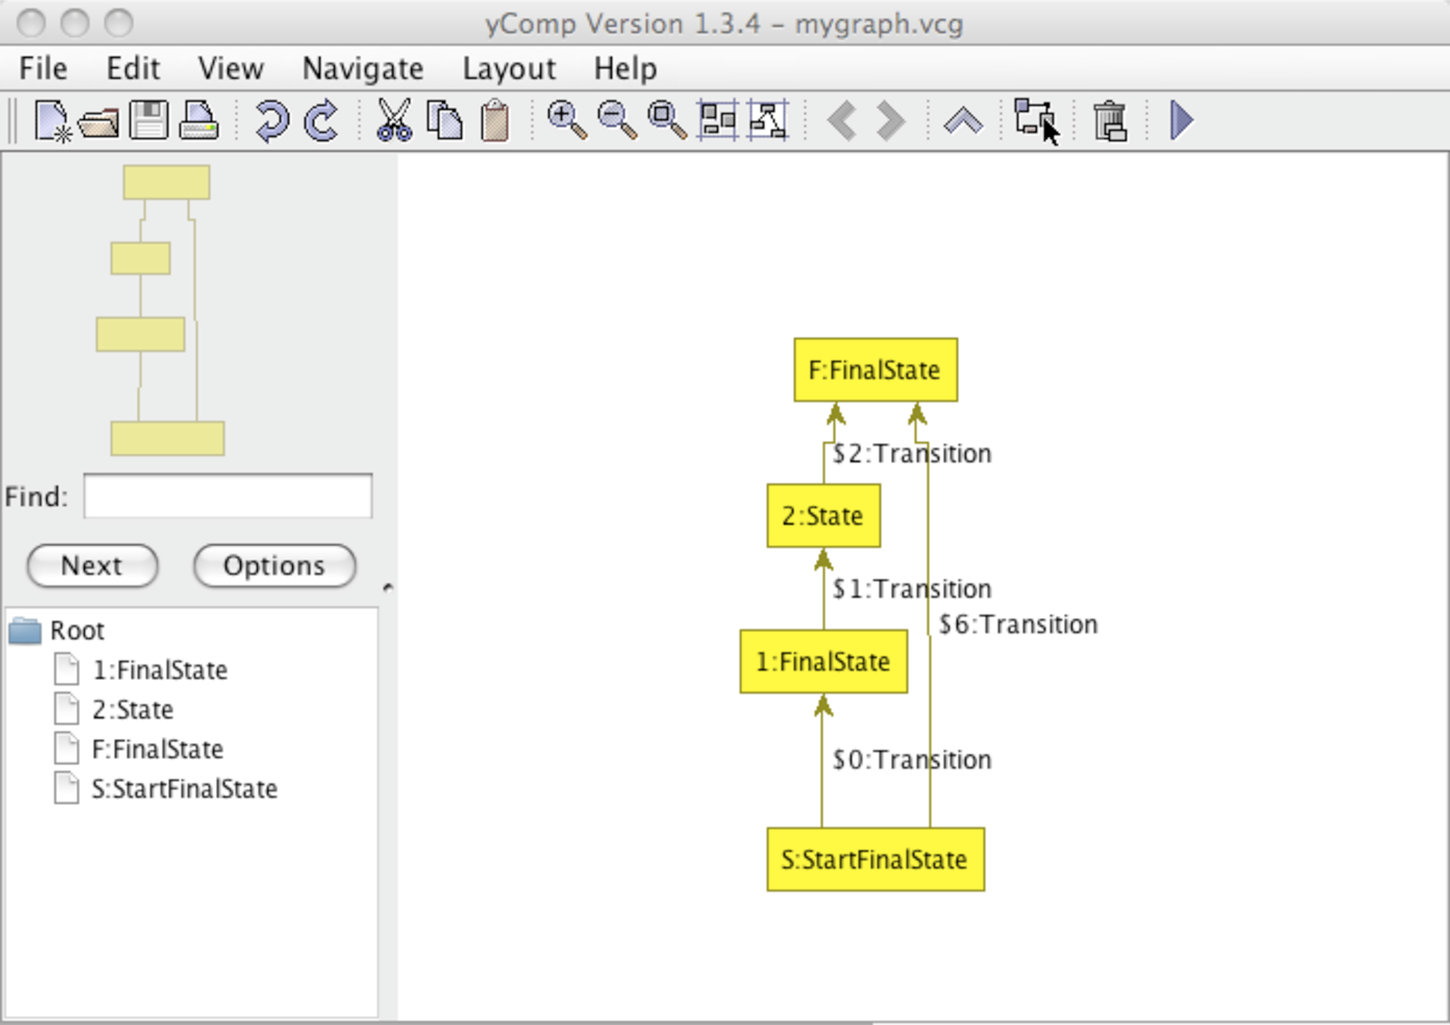
\includegraphics[width=0.8\linewidth]{fig/quickfinal}
	\caption{A state machine without $\varepsilon$-transitions}
	\label{fig:quick:final}
\end{figure}

If everything is working fine you can delete the \texttt{debug} keyword in front of \texttt{xgrs}.
Maybe you want to save the resulting graph.
This is possible by typing \texttt{dump graph mygraph.vcg} in the \GrShell.
\GrShell\ writes the graph in \texttt{mygraph.vcg} into the current directory.
Files in VCG format are readable by \yComp.
Feel free to browse the \texttt{examples} folder shiped with \GrG\ and have a look at further capabilities of the software.


\chapter{Graph Model Language}
\label{chapmodellang}
The key features of \GrG\ graph models from \cite{geiss}:

\begin{description}
\item[Types.] Nodes and edges can have types (classes). This is similar to common programming languages, except \GrG\ types have no concept of methods. 
\item[Attributes.] Nodes and edges can possess attributes. The set of attributes assigned to a node or edge is determined by its type. The attributes themselves are typed, too.
\item[Inheritance.] Types (classes) can be composed by multiple inheritance. \emph{Node} and \emph{Edge} are built-in root types of node and edge types, respectively. Inheritance eases the specification of attributes, because subtypes inherit the attributes of their super types. Note that \GrG\ lacks a concept of overwriting. On a path in the type hierarchy graph from a type up to the built-in root type there must be exactly one declaration for each attribute identifier.
\item[Connection Assertions.] To specify that certain edge types should only connect specific nodes, we include connection assertions. Furthermore the number of outgoing and incoming edges can be constrained.
\end{description}

\begin{figure}[htbf]
\begin{example}\label{ex:model:map}
The following toy example of a model of street maps gives a rough picture of the language:
\begin{grgen}
model Map;

enum resident {village = 500, town = 5000, city = 50000}

node class sight;

node class city {
	size: resident;
}

const node class metropolis extends city {
  river: string;
}  

abstract node class abandoned_city extends city;
node class ghost_town extends abandoned_city;

edge class street;
edge class trail extends street;
edge class highway extends street
    connect metropolis [+] -> metropolis [+]
{
    jam: boolean;
}
\end{grgen}
\end{example}
\end{figure}
In this chapter as well as in the \GrShell\ chapter \ref{chapgrshell} we use excerpts of example~\ref{ex:model:map} (the \texttt{Map} model) for further descriptions.

\section{Building Blocks}
\label{modelbb}

\begin{note}
The following syntax specifications make heavy use of syntax diagrams (also known as rail diagrams). Syntax diagrams provide a visualization of EBNF\footnote{Extended Backus–Naur Form.} grammars. Follow a path along the arrows from left to right through a diagram to get a valid sentence (or sub sentence) of the language. Ellipses are terminals whereas rectangles are non-terminals. For further information on syntax diagrams see \cite{pascal}.
\end{note}
Basic elements of the \GrG\ graph model language are identifiers to denominate types, attributes, and the model itself. The \GrG\ graph model language is case sensitive.\\
\\
\emph{Ident}, \emph{IdentDecl}\\ \nopagebreak
A non-empty character sequence of arbitrary length consisting of letters, digits or underscores. The first character must not be a digit. \emph{Ident} and \emph{IdentDecl} differ in their role: While \emph{IdentDecl} is a \emph{defining} occurrence of an identifier, \emph{Ident} is a \emph{using} occurrence. An \emph{IdentDecl} non-terminal can be annotated. See \ref{annotations} for annotations of declarations.
\begin{note}
  The \GrG\ model language does not distinguish between declarations and definitions. More precisely, every declaration is also a definition. For instance, there are no C-like constructs as the following:
\begin{grgen}
node class t_node;
node class t_node {
}
\end{grgen}
\end{note}
\mbox{ }\\
\emph{NodeType}, \emph{EdgeType}, \emph{EnumType}\\ \nopagebreak
These are (semantic) specializations of Ident to restrict an identifier to be of a specific type.

\section{Type Declarations}
\begin{rail}
  GraphModel: 'model' IdentDecl ';' (() + TypeDeclaration);
\end{rail}
The graph model consists of its name \emph{IdentDecl} and type declarations defining specific node and edge types as well as enums.

\begin{rail}
  TypeDeclaration: EnumDeclaration | ClassDeclaration
\end{rail}
\emph{ClassDeclaration} defines a node or an edge. \emph{EnumDeclaration} defines an enum type for use as attribute of nodes or edges. Types do not need to be declared before they are used.

\begin{rail}
  EnumDeclaration: 'enum' IdentDecl lbrace ((IdentDecl (() | '=' IntExpr)) + ',') rbrace ;
\end{rail}
Defines an enum type.

\begin{example}
\begin{grgen}
enum Color {red, green, blue}
enum Resident {village = 500, town = 5000, city = 50000}
enum AsInC {a = 2, b, c = 1, d, e = Resident::village + c}
\end{grgen}
The semantics is as it is in C \cite{isoc}. So the following holds: $\text{red} = 0$, $\text{green} = 1$, $\text{blue} = 2$, $\texttt{a}=2$, $b=3$, $c=1$, $d=2$, and $e=501$.
\end{example}

\begin{rail}  
  ClassDeclaration: (() | 'abstract') (() | 'const') (NodeClass | EdgeClass);
\end{rail}
Defines a new node type or edge type.\\
The keyword \texttt{abstract} indicates that you cannot instantiate graph elements of this type but rather you have to derive non-abstract types for graph elements. The abstract-property will not be inherited by subclasses.

\begin{example}
We adjust our map model and make \texttt{city} abstract:
\begin{grgen}
abstract node class city {
	size: int;
}
abstract node class abandoned_city extends city;
node class ghost_town extends abandoned_city;
\end{grgen}
You will be able to create nodes of type \texttt{ghost\_town}, but not of type \texttt{city} or \texttt{abandoned\_city}. However, nodes of type \texttt{ghost\_town} are also nodes of type \texttt{abandoned\_city} and of type \texttt{city} and they have the attribute \texttt{size}.
\end{example}
The keyword \texttt{const} indicates that rules may not write to attributes. See also \ref{replacepart}, \texttt{eval}. However, attributes are writable by \LibGr\ and \GrShell\ directly. This property will not be inherited by subclasses. If you want a subclass to have constant attributes, you have to set the \texttt{const} modifier explicitly.

\begin{rail}  
  NodeClass: 'node' 'class' IdentDecl (() | 'extends' (NodeType+',')) \\ 
    (';' | lbrace AttributeDeclarations rbrace);
\end{rail}
Defines a new node type. Node types can inherit from other node types defined within the same file. If the \texttt{extends} clause is omitted, \emph{NodeType} will inherit from the built-in type \texttt{Node}. Optionally nodes can possess attributes.

\begin{rail}    
  EdgeClass: 'edge' 'class' IdentDecl (() | 'extends' (EdgeType+',')) \\
    (() + ConnectAssertions) (';' | lbrace AttributeDeclarations rbrace);
\end{rail}
Defines a new edge type. Edge types can inherit from other edge types defined within the same file. If the \texttt{extends} clause is omitted, \emph{EdgeType} will inherit from the built-in type \texttt{Edge}. Optionally edges can possess attributes. A \emph{connection assertion} specifies that certain edge types should only connect specific nodes and, moreover, the number of outgoing and incoming edges can be constrained.

\begin{rail}  
  ConnectAssertions: 'connect' (NodeConstraint '->' NodeConstraint + ',');
  NodeConstraint: NodeType (() | '[' ('*' | '+' | Number | RangeConstraint) ']') ;
  RangeConstraint: Number ':' ('*' | Number) ;
\end{rail}
A connection assertion is typed as a pair of node types in conjunction with their multiplicities. A corresponding edge may connect a node of the first node type or one of its subtypes (source) with a node of the second node type or one of its subtypes (destination). The multiplicity is a constraint on the out-degree and in-degree of the source and destination node type respectively. \emph{Number} is an \texttt{int} constant as defined in section \ref{expressions}. See \ref{graphcommands}, \texttt{validate}, for an example. Table \ref{multiplicities} describes the multiplicity definitions.
\begin{table}[htbp]
\begin{tabularx}{\linewidth}{|l|X|}\hline
	\texttt{[n:*]} & The number of edges nodes of that type are incident to is unbounded. At least $n$ edges must be incident to nodes of that type.\\ 
	\texttt{[n:m]} & At least $n$ edges must be incident to nodes of that type, but at most $m$ edges may be incident to nodes of that type ($m \geq n$ must hold).\\
	\texttt{[*]} & Abbreviation for \texttt{[0:*]}.\\
	\texttt{[+]} & Abbreviation for \texttt{[1:*]}\\
	\texttt{[n]} & Abbreviation for \texttt{[n:n]}. \\ \hline
\end{tabularx}
\caption{\GrG\ node constraint multiplicities concerning a specific pair of an edge type and a node type.}
\label{multiplicities}
\end{table}

\begin{rail}    
  AttributeDeclarations: (() | IdentDecl ':' AttributeType ';') + ;
  AttributeType: PrimitiveType | EnumType ; 
\end{rail}
Defines a node or edge attribute. Possible types are \texttt{enum} and primitive types. See \ref{builtin} for a list of built-in primitive types.




\chapter{Rule Set Language}\indexmain{rule set language}
\label{chaprulelang}

The \indexed{rule set} language forms the core of \GrG. Rule files refer to zero\footnote{Omitting a graph meta model means that \GrG\ uses a \indexed{default graph model}. The default model consists of the base type \texttt{Node} for vertices and the base type \texttt{Edge} for edges.} or more \indexed{graph model}s and specify a set of rewrite rules. The rule language covers the pattern specification and the replace/modify specification. Attributes of graph elements can be re-evaluated during an application of a rule. The following rewrite rule mentioned in Geiß et al.~\cite{GBGHS:06} gives a rough picture of the language:
%\begin{figure}[tb]
\begin{example}\label{ex:rule:SomeRule}
\begin{grgen}
using SomeModel;

rule SomeRule {
  n1:NodeTypeA;
  n2:NodeTypeA;
  hom(n1, n2);
  n1 --> n2; /*@\label{ex:somerule:graphlet}@*/
  n3:NodeTypeB;
  negative {
    n3 -e1:EdgeTypeA-> n1;
    if {n3.a1 == 42*n2.a1;}
  }
  negative { /*@\label{ex:somerule:secondnac:begin}@*/
    n4:Node\(NodeTypeB);
    n3 -e1:EdgeTypeB-> n4;
    if {typeof(e1) >= EdgeTypeA;}
  } /*@\label{ex:somerule:secondnac:end}@*/
  replace {
    n5:NodeTypeC<n1>;
    n3 -e1:EdgeTypeB-> n5;
    eval {n5.a3 = n3.a1*n1.a2;}
  }  
}
\end{grgen}
\end{example}
%\end{figure}
In this chapter we use excerpts of Example~\ref{ex:rule:SomeRule} (\texttt{SomeRule}) for illustration purposes.
The nested negative which specify a pattern which must not be available in the host graph are described in the following chapter \ref{cha:nestedsub}

\section{Building Blocks}
\label{rulebb}

The \GrG\ rule set language is \indexed{case sensitive}. The language makes use of several identifier specializations in order to denominate all the \GrG\ entities.\\
\\
\emph{Ident}, \emph{IdentDecl}\\ \indexmain{identifier}\nopagebreak
A non-empty character sequence of arbitrary length consisting of letters, digits, or underscores. The first character must not be a digit. \emph{Ident} may be an identifier defined in a graph model (see Section~\ref{modelbb}). \emph{Ident} and \emph{IdentDecl} differ in their role: While \emph{IdentDecl} is a \emph{defining} occurrence of an identifier, \emph{Ident} is a \emph{using} occurrence. An \emph{IdentDecl} non-terminal can be annotated\indexmain{annotation}. See Section~\ref{annotations} for annotations of declarations.
\begin{note}
  As in the \GrG\ model language (see note~\ref{note:modeldecl}) every declaration is also a definition. Using an identifier before defining it is allowed. Every used identifier has to be defined exactly once.
\end{note}
\mbox{ }\\
\emph{ModelIdent}, \emph{TypeIdent}, \emph{NodeType}, \emph{EdgeType}\\
These are (semantic) specializations of \emph{Ident}. \emph{TypeIdent} matches every type identifier, i.e.\ a node type, an edge type, an enumeration type or a primitive type. All the type identifiers are actually type \emph{expressions}\indexmain{type expression}. See Section~\ref{typeexpressions} for the use of type expressions.\\

\subsection{Graphlets}
\label{sct:graphlets}
\begin{rail}
  Graphlet: (GraphletNode (() | Continuation) | Continuation) ';' ;
  Continuation: GraphletEdge (() | (GraphletNode (() | Continuation))) ;
\end{rail}\ixnterm{Graphlet}\ixnterm{Continuation}
A \indexed{graphlet} specifies a connected subgraph. 
\GrG\ provides graphlets as a descriptive notation to define both, patterns\indexmain{pattern graph} to search for as well as the subgraphs that replace or modify matched \indexed{spot}s in a host graph\indexmain{replacement graph}. 
Any graph can be specified piecewise by a set of graphlets. 
In Example~\ref{ex:rule:SomeRule}, line~\ref{ex:somerule:graphlet}, the statement \texttt{n1 --> n2} is the node identifier \texttt{n1} followed by the \indexedsee{continuation}{graphlet} graphlet \texttt{--> n2}.

All the graph elements of a graphlet have \newterm{name}s.
The name is either user-assigned or a unique internal, non-accessible name.
In the second case the graph element is called \newterm{anonymous}.
For illustration purposes we use a \indexed{\texttt{\$<number>}} notation to denote anonymous graph elements in this document.
For example the graphlet \texttt{n1 --> n2} contains an anonymous edge; thus can be understood as \texttt{n1 -\$1:Edge-> n2}.
Names must not be \indexed{redefine}d; once defined, a name is \emph{bound} to a graph element. 
We use the term ``\indexed{binding of names}'' because a name not only denotes a graph element of a graphlet but also denotes the mapping of the abstract graph element of a graphlet to a concrete graph element of a host graph.
So graph elements of different names are pair wise distinct except for homomorphically matched\indexmain{homomorphic matching} graph elements (see Section~\ref{patternpart}).
For instance \texttt{v:NodeType1 -e:EdgeType-> w:NodeType2} selects some node of type \texttt{Node\-Type1} that is connected to a node of type \texttt{NodeType2} by an edge of type \texttt{EdgeType} and binds the names \texttt{v}, \texttt{w}, and \texttt{e}. 
If \texttt{v} and \texttt{w} are not explicitly marked as homomorphic, the graph elements they bind to are distinct.
Binding of names allows for splitting a single graphlet into multiple graphlets as well as defining cyclic structures.
\begin{example}
The following graphlet (\texttt{n1}, \texttt{n2}, and \texttt{n3} are defined somewhere else)
\begin{grgen}
n1 --> n2 --> n3 <-- n1;
\end{grgen}
is equivalent to
\begin{grgen}
n2 --> n3;
n1 --> n2;
n3 <-- n1;
\end{grgen}
and \texttt{n1 --> n3} is equivalent to \texttt{n3 <-- n1}, of course.
\end{example}
The visibility of names is determined by \indexed{scope}s. 
Scopes can be nested. 
Names of surrounding scopes are visible in inner scopes. 
Usually a scope is defined by \texttt{\{} and \texttt{\}}. %In contrast to pure syntactic scoping, the replace/modify part is a direct inner scope of the pattern part.
In Example~\ref{ex:rule:SomeRule}, lines~\ref{ex:somerule:secondnac:begin}~to~\ref{ex:somerule:secondnac:end}, the negative condition uses \texttt{n3} from the surrounding scope and defines \texttt{n4} and \texttt{e1}. 
We may safely reuse the variable name \texttt{e1} in the replace part.

\begin{rail}
GraphletNode: (Ident | 
    '.' |
    (() | IdentDecl) ':' NodeType (() | TypeConstraint | Retyping)) ;   
\end{rail}\ixnterm{GraphletNode}
Specifies a node\indexmain{node (graphlet)} of type \emph{NodeType},
maybe constrained in type with a \emph{TypeConstraint}\indexmain{type constraint} (see Section~\ref{typehandling}, \emph{TypeConstraint}),
maybe retyped with a \emph{Reytping}\indexmain{retype} (see Section~\ref{typehandling}, \emph{Retyping}).
The \texttt{.}\ is an anonymous node of the base type \texttt{Node}; remember that every node type has \texttt{Node} as super type. 
Type constraints are allowed in the pattern part only. 
Retyping is allowed in the replace/modify part only.
\begin{center}
  \begin{tabularx}{\linewidth}{lX}
    \textbf{Graphlet} & \textbf{Meaning}\\ \hline
    \texttt{x:NodeType;} & The name \texttt{x} is bound to a node of type \texttt{NodeType} or one of its subtypes. \\
    \texttt{ :NodeType;} & \texttt{\$1:NodeType} \\
    \texttt{.;} & \texttt{\$1:Node} \\
    \texttt{x;} & The node, \texttt{x} is bound to.
  \end{tabularx}
\end{center} 

\begin{rail}
  GraphletEdge: '-' EdgeRefinement '->'  | '<-' EdgeRefinement '-'  | '<-' EdgeRefinement '->' | '?-' EdgeRefinement '-?' ;
  EdgeRefinement: () | Ident | (() | IdentDecl) ':' EdgeType (() | TypeConstraint | Retyping) ;
\end{rail}\ixnterm{GraphletEdge}\ixnterm{EdgeRefinement}
A \emph{GraphletEdge} specifies an edge\indexmain{edge (graphlet)}. 
Anonymous edges are specified by an empty \emph{EdgeRefinement} clause, i.\,e.\ \texttt{-->}, \texttt{<--}, \texttt{<-->}, \texttt{--}, \texttt{?--?} or \texttt{-:T->}, \texttt{<-:T-}, \dots\ for an edge type \texttt{T}, respectively. 
A non-empty \emph{EdgeRefinement} clause allows for detailed edge type specification. 
Type constraints\indexmain{type constraint} are allowed in the pattern part only (see Section~\ref{typehandling}, \emph{TypeConstraint}).
Retyping is allowed in the replace/modify part only (see Section~\ref{typehandling}, \emph{Retyping}).

The different kind of arrow tips distinguish between \indexed{directed}, \indexed{undirected}, and \indexed{arbitrary} edges (see also Section~\ref{sct:basetypes}).
The arrows \texttt{-->} and \texttt{<--} are used for directed edges with a defined source and target.
The arrow \texttt{--} is used for undirected edges.
The pattern part allows for further arrow tips, namely \texttt{?--?}\ for arbitrary edges and \texttt{<-->} for directed edges with undefined direction.
Note that \texttt{<-->} is \emph{not} equivalent to the \texttt{--> ; <-- ;} statements.
In order to produce a match for the arrow \texttt{<-->}, it is sufficient that one of the statements \texttt{-->}, \texttt{<--} matches.
If an edge type is specified (through the \emph{EdgeRefinement} clause), this type has to correspond to the arrow tips, of course.
\begin{center}
	\begin{tabularx}{\linewidth}{lX}
		\textbf{Graphlet} & \textbf{Meaning}\\ \hline
		\texttt{ -e:EdgeType-> ;} & The name \texttt{e} is bound to an edge of type \texttt{EdgeType} or one of its subtypes. \\
		\texttt{ -:EdgeType-> ;} & \texttt{-\$1:EdgeType-> ;} \\
		\texttt{ --> ;} & \texttt{-\$1:Edge-> ;} \\
		\texttt{ <--> ;} & \texttt{-\$1:Edge-> ;} or  \texttt{<-\$1:Edge- ;}\\
		\texttt{ -- ;} & \texttt{-\$1:UEdge-> ;} \\
		\texttt{ ?--?\ ;} & \texttt{-\$1:AEdge-> ;} \\
		\texttt{ -e-> ;} & The edge, \texttt{e} is bound to.
	\end{tabularx}
\end{center} 
As the above table shows, edges can be defined and used separately, i.e.\ without their incident nodes. Beware of accidentally ``\indexed{redirecting}''\footnote{You cannot directly express the redirection of edges. This a direct consequence of the \indexedsee{SPO}{single-pushout approach}\indexmain{single-pushout approach} approach. Redirection of edges can be ``simulated'' by either deleting and re-inserting an edge, or more indirect by re-typing of nodes.} an edge: 
The graphlets
\begin{grgenlet}
-e:Edge-> .;
x:Node -e-> y:Node;
\end{grgenlet}
are illegal, because the edge \texttt{e} would have two destinations: an anonymous node and \texttt{y}.
However, the graphlets
\begin{grgenlet}
-e-> ;
x:Node -e:Edge-> y:Node;
\end{grgenlet}
are allowed, but the first graphlet \texttt{-e->} is superfluous. In particular this graphlet does not identify or create any ``copies'', neither if the graphlet occurs in the pattern part nor if it occurs in the replace part.
\begin{example}
Some attempts to specify a loop edge:\\
\mbox{ }\\
\begin{tabular}[c]{ll} 
 \textbf{Graphlet} & \textbf{Meaning} \\ \hline
 \texttt{x:Node -e:Edge-> x;} & The edge \texttt{e} is a loop.\\ 
 \texttt{x:Node -e:Edge-> ; -e-> x;} & The edge \texttt{e} is a loop.\\ 
 \texttt{-e:Edge-> x:Node;} & The edge \texttt{e} may or may not be a loop.\\ 
 \texttt{.\ -e:Edge-> .;} & The edge \texttt{e} is certainly not a loop.\\ 
\end{tabular}
\end{example}

\begin{figure}[htbp]
\begin{example}
\label{ex:somegraphlets}
Some graphlets:

\begin{center}
\begin{tabular}[c]{cl}
  & \\
  \begin{tabular}[c]{c}\begin{tikzpicture}
      \tikzstyle{every node}=[circle]
      \node[draw] (n1) at (1,0) {};
      \node[draw] (n2) at (2,1) {};
      \node[draw] (n3) at (1,2) {};
      \node[draw] (n4) at (0,1) {};
    	
      \draw[-latex] (n3) .. controls +(-1,0) .. (n4) {};
      \draw[-latex] (n4) .. controls +(0,-1) .. (n1) {};
      \draw[-latex] (n1) .. controls +(1,0) .. (n2) {};
      \draw[-latex] (n2) .. controls +(0,1) .. (n3) {};
    \end{tikzpicture}\end{tabular} & \begin{tabular}[c]{l} \texttt{x:Node --> .\ --> .\ --> .\ --> x;} \end{tabular}\\
  & \\  
  \begin{tabular}[c]{c}\begin{tikzpicture}
      \tikzstyle{every node}=[circle]
      \node[draw] (n1) at (1,1) {};
      \node[draw] (n2) at (0,0) {};
      \node[draw] (n3) at (0,2) {};
      \node[draw] (n4) at (2,0) {};
      \node[draw] (n5) at (2,2) {};
    	
      \draw[-latex] (n1) -- (n2) {};
      \draw[-latex] (n1) -- (n3) {};
      \draw[-latex] (n1) -- (n4) {};
      \draw[-latex] (n1) -- (n5) {};
    \end{tikzpicture}\end{tabular} & \begin{tabular}[c]{l} \texttt{.\ <-- x:Node --> .;} \\ \texttt{.\ <-- x --> .;} \end{tabular}\\
  & \\
  \begin{tabular}[c]{c}\begin{tikzpicture}
      \tikzstyle{every node}=[circle]
      \node[draw] (n1) at (3,5) {};
      \node[draw] (n2) at (2,4)   {};
      \node[draw] (n3) at (0,2)   {};
      \node[draw] (n4) at (2,0)   {};
      \node[draw] (n5) at (4,2)   {};
      \node[draw] (n6) at (2,5.0)   {};
    	
    	\draw[-latex] (n2) --                                  (n1) node[right,pos=0.6] {$e_1:\text{stem}$};
    	\draw[-latex] (n2) .. controls +(-1,1) and +(0,1) ..   (n3) node[left,midway]  {$e_2$};
      \draw[-latex] (n3) .. controls +(0,-1) and +(-1,0) ..  (n4) node[left,midway]  {$e_3$};
    	\draw[-latex] (n4) .. controls +(1,0)  and +(0,-1) ..  (n5) node[right,midway] {$e_4$};
      \draw[-latex] (n5) .. controls +(0,1)  and +(1,1) ..   (n2) node[right,midway] {$e_5$};
    	\draw[-latex] (n2) .. controls +(-0.3,+0.3) and +(-0.3,-0.3) .. (n6) node[left,midway]   {};
    	\draw[-latex] (n2) .. controls +(+0.3,+0.3) and +(+0.3,-0.3) .. (n6) node[right,midway]  {};
    \end{tikzpicture}\end{tabular} & \begin{tabular}[c]{l} \texttt{.\ <-e1:stem- n1:Node -e2:Edge-> .\ -e3:Edge-> .} \\ \quad\texttt{-e4:Edge-> .\ -e5:Edge-> n1;}\\ \texttt{n1 --> n2:Node;} \\ \texttt{n1 --> n2;} \end{tabular}\\
   & \\
  \begin{tabular}[c]{c}\begin{tikzpicture}
      \tikzstyle{every node}=[circle]
      \node[draw] (n1) at (0,0) {};
      \node[draw] (n2) at (1,0) {};
      \node[draw] (n3) at (2,0) {};
      \node[draw] (n4) at (3,0) {};
      \node[draw] (n5) at (4,0) {};
    	
      \draw[-latex] (n1) -- (n2) {};
      \draw[-latex] (n3) -- (n2) {};
      \draw[-latex] (n4) -- (n3) {};
      \draw[-latex] (n4) -- (n5) {};
    \end{tikzpicture}\end{tabular} & \begin{tabular}[c]{l} \texttt{.\ --> .\ <-- .\ <-- .\ --> .;} \end{tabular} \\
  & \\
  \begin{tabular}[c]{c}\begin{tikzpicture}
      \tikzstyle{every node}=[circle]
      \node (n1) at (0,0) {};
      \node[draw] (n2) at (1,0) {};
      \node[draw] (n3) at (2,0) {};
      \node (n4) at (3,0) {};
    	
      \draw[-latex] (n2) -- (n1) {};
      \draw[-latex] (n3) -- (n2) node[midway,above] {$e$};
      \draw[-latex] (n3) -- (n4) {};
    \end{tikzpicture}\end{tabular} & \begin{tabular}[c]{l} \texttt{-e:Edge->} \\ \texttt{<-- .\ <-e- .\ -->\ ;} \end{tabular}
\end{tabular}\\
\end{center}
\mbox{ }\\
\mbox{ }\\
\mbox{ }\\
And some illegal graphlets:\\
\mbox{}\\
\mbox{}\\
\begin{tabularx}{\linewidth}{cX}
\texttt{.\ -e:Edge-> .; .\ -e-> .;} & Would affect redirecting of edge \texttt{e}. \\
 & \\
 \texttt{x -e:T-> y; x -e-> x;} & Would affect redirecting of edge \texttt{e}. \\
 & \\
 \texttt{<-- --> ;} & There must be at least a node between the edges.
\end{tabularx}
\end{example}
\end{figure}

\begin{note}
	Although both, the pattern part and the replace/modify part use graphlets, there are subtle differences between them. 
	These concern the \emph{TypeConstraint} and \emph{Retyping} clause plus the allowed arrow tips for edges.
\end{note}

\section{Rules and Tests}
\label{ruledecls}
The structure of a \indexed{rule set} file is as follows:
\begin{rail}
  RuleSet: Header ((TestDeclaration | RuleDeclaration | SubpatternDeclaration)+) ;
  Header: ('using' ((ModelIdent)+',') ';')? (('\#include' Filename)*());
\end{rail}\ixkeyw{using}\ixnterm{RuleSet}

A rule set consists of the underlying \indexed{graph model}s and several rewrite rules and tests (subpatterns will be introduced in \ref{sec:subpattern}).
Additionally you may include further rule set files (without \texttt{using} directives, we prefer to suffix them with \textt{.gri} in this case).
In case of multiple graph models, \GrG\ uses the union of these models. In this case beware of conflicting declarations.
There is no built-in conflict resolution mechanism like packages or namespaces for models.
If necessary you can use prefixes as you might do in C.

\begin{rail}
  TestDeclaration: 'test' (() | 'exact' | 'induced') ActionSignature lbrace Pattern rbrace ;
  RuleDeclaration: 'rule' (() | 'exact' | 'induced' | 'dpo') ActionSignature lbrace Pattern Replace rbrace ;
\end{rail}\ixkeyw{test}\ixkeyw{rule}\ixkeyw{exact}\ixkeyw{induced}\ixkeyw{dpo}\ixnterm{TestDeclaration}\ixnterm{RuleDeclaration}
Declares a single \indexed{rewrite rule} such as \texttt{SomeRule}. 
It consists of a pattern part (see Section~\ref{patternpart}) in conjunction with its rewrite/modify part (see Section~\ref{replacepart}). 
A \newterm{test} has no rewrite specification. 
It's intended to check whether (and maybe how many times) a pattern occurs (see example \ref{ex:rulelang:testrule}).
For an explanation of the \texttt{exact}, \texttt{induced}, and \texttt{dpo} pattern modifiers see section \ref{sct:patternmodifier}. 
\begin{example}
\label{ex:rulelang:testrule}
We define a test \texttt{SomeCond}
\begin{grgen}
test SomeCond {
  n:SeldomNodeType;
}
\end{grgen}
and execute in \GrShell:
\begin{grshell}
  grs SomeCond & SomeRule
\end{grshell}
SomeRule will only be executed, if a node of type \texttt{SeldomNodeType} exists. 
For graph rewrite sequences in \GrShell\ see Section~\ref{grsthings}.
\end{example}

\begin{rail}  
  ActionSignature: IdentDecl (() | Parameters) (() | ':' ReturnTypes) ;
\end{rail}\ixnterm{ActionSignature}
The \indexed{signature} sets the name of a rewrite rule to \emph{IdentDecl} and optionally names and types of formal \indexed{parameter}s as well as a list of \indexed{return type}s.
Parameters and return types provide users with the ability to exchange graph elements between rules, similar to parameters of procedural languages.
This way it is possible to specify \emph{where} a rule should be applied.

\begin{rail}
  Parameters: '(' (Parameter * ',') ')' ;
  Parameter: IdentDecl ':' NodeType (InputTypeSpecification)? | '-' IdentDecl ':' EdgeType (InputTypeSpecification)? '->' | 'var' IdentDecl ':' VarType ;
  InputTypeSpecification: '<' (NodeEdgeType | 'null' | NodeEdgeType '+' 'null' | 'null' '+' NodeEdgeType ) '>' ;
\end{rail}\ixnterm{Parameters}

Within a rule, graph element parameters are treated as graph elements of the pattern - just predefined.
But in contrast to pervious versions it is the task of the user to ensure the elements handed in satisfy the interface, i.e. parameters must not be null and must be of the type specified or a subtype of the type specified. 
If you need more flexibility and want to call the rule with parameters not fullfilling the interface you can append an input type specification to the relevant parameters, which consists of the type to accept at the action interface, or null, or both, enclosed in left and right angles. 
If the input type specification type is given, but the more specific pattern element type is not satisfied, matching simply fails.
If null is declared in the input type specification and given at runtime, the element is searched in the host graph.
Don't use null parameters unless you need them, because every null parameter doubles the number of matcher routines which get generated.
Non-graph element parameters must be prefixed by the \texttt{var}-keyword, VarType is one of the attribute types supported by \GrG (\ref{built-in-types}).
Please not that the effect of assigning to a var parameter in \texttt{eval}\ref{eval} is undefined (concerning the parameters as well as the argument).

\begin{figure}[htbp]
\begin{example}
The \indexed{test} \texttt{t} that checks whether node \texttt{n1} is \indexed{adjacent} to \texttt{n2} (connected by an undirected edge or incoming directed edge or outgoing directed edge)
\begin{grgen}
test t(n1:Node<null>, n2:Node<null>) {
  n1 ?--? n2;
}
\end{grgen}
is equivalent to the tests \texttt{t1}-\texttt{t4} which are chosen dependent on what parameters are defined.
\begin{grgen}
test t1(n1:Node, n2:Node) {
  n1 ?--? n2;
}
test t2(n1:Node) {
  n1 ?--? n2:Node;
}
test t3(n2:Node) {
  n1:Node ?--? n2;
}
test t4 {
  n1:Node ?--? n2:Node;
}
\end{grgen}
So if both parameters are not defined, \texttt{t4} is chosen, which succeeds as soon as there are two distinct nodes in the graph connected by some edge.
\end{example}
\end{figure}

\begin{rail}
  ReturnTypes: '(' ((NodeType | EdgeType | VarType) + ',') ')' ;
\end{rail}\ixnterm{ReturnTypes}
The return types specify edge and node types of graph elements that are returned by the replace/modify part. If return types are specified, the \texttt{return} statement is mandatory. Otherwise no \texttt{return} statement must occur. See also Section~\ref{replacepart}, \texttt{return}.

\begin{figure}[htbp]
\begin{example}\label{ex:rule:someruleext}
We extend \texttt{SomeRule} (Example~\ref{ex:rule:SomeRule}) with a user defined node to match and we want it to return the rewritten graph elements \texttt{n5} and \texttt{e1}.
\begin{grgen}
  rule SomeRuleExt(varnode:Node):(Node, EdgeTypeB) {
    n1:NodeTypeA;
    ...
    
    replace {
      varnode;
      ...  
      return(n5, e1);
      eval {
        ...
\end{grgen}
We do not define \texttt{varnode} within the pattern part because this is already covered by the parameter specification itself.
\end{example}
\end{figure}

\section{Pattern Part}\indexmain{pattern}
\label{patternpart}
%\begin{rail}
%  Pattern: (() + ('exact' | 'induced')) 'pattern' lbrace (()+PatternStatement) rbrace ;
%\end{rail}\ixkeyw{pattern}\ixkeyw{induced}\ixnterm{Pattern}
\begin{rail}
  Pattern: (()+PatternStatement) (() | ReturnStatement);
\end{rail}
A \indexed{pattern} consists of zero or more pattern statements and, in case of a test, an optional return statement.
All the pattern statements must be fulfilled by a subgraph of the host graph in order to form a match. 
An \indexed{empty pattern} always produces exactly one (empty) match. 
This is caused by the uniqueness of the total and totally undefined function.
For an explanation of the pattern modifiers \texttt{dpo}, \texttt{induced}, and \texttt{exact} see section~\ref{sct:patternmodifier}.

Names defined for graph elements may be used by other pattern statements as well as by replace/modify statements. 
Like all identifier definitions, such names may be used before their \indexed{declaration}. 
See Section~\ref{rulebb} for a detailed explanation of names and graphlets.
\begin{figure}[htbp]
\begin{note}
\label{note:indeterminism}
The \indexed{application} of a rule is not deterministic\indexmain{non-determinism}\indexmainsee{determinism}{non-determinism} (remember the example of the introduction in Section~\ref{ov:example}); in particular there may be more than one subgraph that matches the pattern. 
Whereas the \GrShell\ selects one of them arbitrarily (without further abilities to control the selection), the underlying \LibGr\indexmain{libGr} provides a mechanism to deal with such ambiguities. 

Also notice that graph rewrite \emph{sequences}\indexmain{graph rewrite sequence} introduce a further variant of non-determinism on rule application level: 
The \indexed{\texttt{\$<op>}} flag marks the operator \texttt{<op>} as commutative, i.e.\ the execution order of its operands (rules) is non-deterministic. 
See chapter~\ref{cha:xgrs} for further information on graph rewrite sequences.
\end{note}
\end{figure}

\begin{rail}  
  PatternStatement: 
    Graphlet ';' |
    'hom' '(' (Ident + ',') ')' ';' |
    ('exact' | 'induced') '(' (Ident+',') ')' |
    'if' lbrace (BooleanExpr ';' +) rbrace |
    NestedPattern |
    SubpatternEntityDeclaration
    ;

\end{rail}\ixkeyw{induced}\ixkeyw{exact}\ixkeyw{hom}\ixkeyw{if}\ixnterm{PatternStatement}
The semantics of the various pattern statements are given below:
\begin{description}
  \item[Graphlet] \indexmain{graphlet}Graphlets specify connected subgraphs. See Section~\ref{rulebb} for a detailed explanation of graphlets.
  \item[Isomorphic/Homomorphic Matching] \indexmain{isomorphic matching}\indexmain{homomorphic matching}The \texttt{hom} operator specifies the nodes or edges that may be matched homomorphically. 
  In contrast to the default isomorphic matching, the specified graph elements \emph{may} be mapped to the same graph element in the host graph. Note that the graph elements must have a common subtype. 
  Several homomorphically matched graph elements will be mapped to a graph element of a common subtype.
  In Example~\ref{ex:rule:SomeRule} nodes \texttt{n1} and \texttt{n2} may be the same node. This is possible because they are of the same type (\texttt{NodeTypeA}).
  Inside a NAC the \texttt{hom} operator may only operate on graph elements that are either defined or used in the NAC.
  Nested \texttt{negative}/\texttt{independent} blocks inherit the \texttt{hom} declarations of their nesting pattern.
  In contrast to previous versions \texttt{hom} delarations are non-transitive, i.e \texttt{hom(a,b)} and \texttt{hom(b,c)} don't cause \texttt{hom(a,c)} unless specified.
  \item[Attribute Conditions] \indexmain{attribute condition}The Java-like attribute conditions (keyword \texttt{if}) in the pattern part allow for further restriction of the applicability of a rule.
  \item[Pattern Modifiers] Additionally to modifiers that apply to a pattern as a whole, you may also specify pattern modifiers for a specific set of nodes. Accordingly the list of identifiers for a pattern modifier must not contain any edge identifier. See section \ref{sct:patternmodifier} for an explanation of the \texttt{exact} and \texttt{induced} modifiers. 
  \item[NestedPattern] will be explained in \ref{nac},\ref{pac},\ref{cardinality},\ref{alternative}.
  \item[SubpatternEntityDeclaration] will be explained in \ref{sec:subpattern}.
\end{description}

Keep in mind that using type constraints or the \texttt{typeof} operator might be helpful. See Section~\ref{typeexpressions} for further information.


\begin{rail}
  ReturnStatement: 'return' '(' ((Ident|Expression)+',') ')' ';' ;
\end{rail}\ixkeyw{return}\ixnterm{ReturnStatement}
\indexmain{return value}Returned graph elements (given by their name) and value entities (given by an expression computing them) must appear in the same order as defined by the return types in the signature (see Section~\ref{ruledecls}, \texttt{ActionSignature}).
Their types must be compatible to the return types specified.

\begin{note}
If you are using a graph at the API level without shell-provided names accessible by the \texttt{nameof}-operator, you may want to number the graph elements for dumping like this:
\begin{grgen}
rule numberNode(var id:int) : (int)
{
  n:NodeWithIntId;
  if { n.id == 0; }
  
  modify {
    eval {
      n.id = id;
    }
    return (id + 1);
  }
}
\end{grgen}
\end{note} 


\section{Replace/Modify Part}\indexmain{replacement graph}
\label{replacepart}
Besides specifying the pattern, a main task of a rule is to specify the transformation of a matched subgraph within the \indexed{host graph}. 
Such a \indexed{transformation specification} defines the transition from the \indexed{left hand side} (LHS) to the \indexed{right hand side} (RHS), i.e.\ which graph elements of a match will be kept, which of them will be deleted and which graph elements have to be newly created.

\subsection{Implicit Definition of the Preservation Morphism\indexmain{preservation morphism} $r$}
\label{rule:morphismr}
In theory the transformation specification is done by defining the preservation morphism $r$.
\begin{figure}[htbp]
	\centering
  \begin{tikzpicture}
    \begin{scope}[minimum size=0.5cm]
      \tikzstyle{every node}=[draw]
      \node (L)     at (0   ,2.5) {$L$};
      \node (R)     at (7   ,2.5) {$R$};
      \node (mL)    at (0   ,0) {};
      \node (mR)    at (7   ,0) {};
      \node[text width=2cm,text badly ragged,minimum size=1cm] (H)     at (0   ,0) {$H$};
      \node[text width=2cm,text badly ragged,minimum size=1cm] (Hs)    at (7   ,0) {$H'$};
    \end{scope}

    \draw[dotted,->] (L) node[above=0.4cm] {Pattern Graph} -> (mL) node[left,midway]  {Match $m$}   node[below=0.6cm] {Host Graph};
    \draw[dotted,->] (R) node[above=0.4cm] {Rewrite Graph} -> (mR)                              node[below=0.6cm] {Result Graph};

    \pgfsetshortenstart{0.5cm}
    \pgfsetshortenend{0.5cm}
    \draw[thick,->]  (L) -> (R)  node[above,midway] {Preservation Morphism $r$} node[below,midway] {Rule};
    \draw[thick,->]  (H) -> (Hs) node[below,midway] {Rule Application};
  \end{tikzpicture}
  \caption{Process of Graph Transformation}
  \label{rule:figrule}
\end{figure}
In \GrG\, the preservation morphism $r$ is defined implicitly by using \indexed{name}s both in pattern \indexed{graphlet}s and replace graphlets.
Remember that to each of the graph elements a name is bound to, either user defined or internally defined. If such a name is used in a replace graphlet, the denoted graph element will be kept. 
Otherwise the graph element will be deleted.
By defining a name in a replace graphlet a corresponding graph element will be newly created.
So in a replace pattern \indexed{anonymous} graph elements will always be created.
Using a name multiple times has the same effect as a single using occurrence.
In case of a conflict between \indexed{deletion} and \indexed{preservation}, deletion is prioritized. 
If an incident node of an edge gets deleted, the edge will be deleted as well (in compliance to the SPO\indexmain{single-pushout approach} semantics).

\begin{table}[htbp]
\centering
\begin{tabularx}{\linewidth}{lllX}
  \textbf{Pattern (LHS)} & \textbf{Replace (RHS)} & \textbf{$r: L \longrightarrow R$} & \textbf{Meaning} \\ \hline 
  \texttt{x:T;} & \texttt{x;}                 & $r:\lhs.x \mapsto \rhs.x$ & Preservation \\
  \texttt{x:T;} & \texttt{}                   & $\lhs.x \notin \deF(r)$    & Deletion \\
  \texttt{} & \texttt{x:T;}                   & $\rhs.x \notin \ran(r)$    & Creation \\
  \texttt{x:T;} & \texttt{x:T;}               & --- & Illegal, redefinition of \texttt{x} \\
  \texttt{-e:T-> ;} & \texttt{-e-> x:Node;}    & --- & Illegal, redirection of  \texttt{e} \\
  \texttt{x:N -e:E-> y:N;} & \texttt{x -e-> ;} & $r:\{\lhs.x\} \mapsto \{\rhs.x\}$ & Deletion of \texttt{y}. Hence del\-etion of \texttt{e}. \\
\end{tabularx}
\caption{Definition of the preservation morphism $r$}
\label{rule:impldefinition}
\end{table}



\subsection{Specification Modes for Graph Transformation}
For the task of rewriting, \GrG\ provides two different modes: A \emph{replace mode} and a \emph{modify mode}.
\begin{description}
  \item[Replace mode] \indexmain{replace mode}The semantics of this mode is to delete every graph element of the pattern that is not used (occur) in the replace part, keep every graph element that is used, and create every additionally defined graph elements. ``Using'' means that the name of a graph element occurs in a replace graphlet. Attribute calculations are no using occurrences.\\
  In Example~\ref{ex:rule:someruleext} the nodes \texttt{varnode} and \texttt{n3} will be kept. The node \texttt{n1} is replaced by the node \texttt{n5} preserving \texttt{n1}'s edges. The anonymous edge instance between \texttt{n1} and \texttt{n2} only occurs in the pattern and therefore gets deleted.\\
See Section~\ref{rule:morphismr} for a detailed explanation of the transformation semantics. 
  \item[Modify mode] The \indexed{modify mode} can be regarded as a replace part in replace mode, where every pattern graph element is added (occurs) before the first replace statement. 
In particular all the \indexed{anonymous} graph elements are kept. 
Additionally this mode supports the \texttt{delete} operator that deletes every element given as an argument. 
Deletion takes place after all other rewrite operations. Multiple deletion of the same graph element is allowed (but pointless) as well as deletion of just created elements (pointless, too).
\begin{figure}[htbp]
\begin{example}
How might Example~\ref{ex:rule:someruleext} look in modify mode? 
We have to denominate the anonymous edge between \texttt{n1} and \texttt{n2} in order to delete it. 
The node \texttt{varnode} should be kept and does not need to appear in the modify part. 
So we have
\begin{grgen}
rule SomeRuleExtModify(varnode: Node): (Node, EdgeTypeB)  {
  ...
  n1 -e0:Edge-> n2;
  ...
  modify {
    n5:NodeTypeC<n1>;
    n3 -e1:EdgeTypeB-> n5;
    delete(e0);
    eval {
      ...
\end{grgen}
\end{example}
\end{figure}
\end{description}

\subsection{Syntax}

\begin{rail}
  Replace: ('replace' | 'modify') lbrace (()+ReplaceStatement) (() | ReturnStatement) \\
  (()+ExecStatement) rbrace ;
\end{rail}\ixkeyw{replace}\ixkeyw{modify}\ixnterm{Replace}
Selects whether the replace mode or the modify mode is used. Several replace statements describe the transformation from the pattern subgraph to the destination subgraph.

\begin{rail}  
  ReplaceStatement:
    Graphlet ';' |
    'delete' '(' (Ident + ',') ')' ';' |
    'eval' lbrace (Assignment ';' +) rbrace |
    SubpatternRewriteApplication
    ;
\end{rail}\ixkeyw{delete}\ixkeyw{eval}
The semantics of the various replace statements are given below:
\begin{description}
  \item[Graphlet] \indexmain{graphlet}Analogous to a pattern graphlet; a specification of a connected subgraph. Its graph elements are either kept because they are elements of the pattern or added otherwise. Names defined in the pattern part must not be redefined in the replace graphlet. See Section~\ref{rulebb} for a detailed explanation of graphlets. 
  \item[Deletion] \indexmain{deletion}The \texttt{delete} operator is only available in the modify mode. It deletes the specified pattern graph elements. Multiple occurrences of \texttt{delete} statements are allowed. Deletion statements are executed after all other replace statements. Multiple deletion of the same graph element is allowed (but pointless) as well as deletion of just created elements (pointless, too).
  \item[Attribute Evaluation] \indexmain{attribute evaluation}\indexmainsee{evaluation}{attribute evaluation}\indexmainsee{re-evaluation}{attribute evaluation}If a rule is applied, then the attributes of matched and inserted graph elements will be recalculated according to the \texttt{eval} statements.
  \item[SubpatternRewriteApplication] will be explained in \ref{sec:subrule}.
\end{description} 

\begin{rail}    
   Assignment: NodeOrEdge '.' Ident '=' Expression | NodeOrEdge '.' 'visited' ('[' FlagNumber ']')? '=' BoolExpr;
\end{rail}\indexmain{attribute evaluation}\ixnterm{Assignment}
Several evaluation parts are allowed within the replace part. 
Multiple evaluation statements will be internally concatenated, preserving their order.
Evaluation statements have \indexedsee{imperative}{attribute evaluation} semantics.
In particular, \GrG\ does not care about data dependencies.
Evaluation takes place before any graph element gets deleted and after all the new elements have been created.
You may read (and write, although this is pointless) attributes of graph elements to be deleted.
Assignment is carried out using \indexmain{value semantics}, even for entities of \verb#set<K># and \verb#map<K,V># or \texttt{string} type.
The only exception is the type \texttt{object}, there \indexmain{reference semantics} is used.
The \texttt{visited} flag assignment sets the \texttt{boolean} status of the \indexed{visited flag} of the given number for the given graph element.
If no flag number is given, the default number for the first visited flag of 0 is used.
Make sure to allocate\ref{allocvisitflag}/\ref{apiallocvisitflag} visited flags before you try to use them 
(and deallocate them afterwards, as they are a sparse resource stored in some excess bits of the graph elements, or in some dictionary if the needed number of flags exceeds the number of available bits per graph element.)

\begin{example}
\begin{grgen}
...
modify {
  ...
  eval { y.i = 40; }
  eval { y.j = 0;  }
  x:IJNode;
  y:IJNode;
  delete(x);
  eval {
    x.i = 1; 
    y.j = x.i;
    x.i = x.i + 1;
    y.i = y.i + x.i;
  }
}
\end{grgen}
This toy example yields $\texttt{y.i} = 42$, $\texttt{y.j} = 1$.
\end{example}

\section{Rule and Pattern Modifiers}\indexmain{modifier} 
\label{sct:patternmodifier}
By default \GrG\ performs rewriting according to \indexmain{SPO} semantics as explained in section \ref{rule:morphismr}.
This behaviour can be changed with \newterm{rule / pattern modifiers}.
Such modifiers add certain conditions to the applicability of a pattern.
The idea is to match only parts of the host graph that look more or less exactly like the pattern.
The level of ``exactness'' depends on the choosen modifier.
A modifier in front of the \texttt{pattern}-keyword is equivalent to one modifier-statement inside the pattern containing all the specified nodes (including anonymous nodes).
Table \ref{tbl:rules:modifiers} lists the modifiers with their semantics.
Example \ref{ex:rules:modifiers} explains the modifiers by small toy-graphs.
\begin{note}
    Internally all the modifier-annotated rules are resolved into equivalent rules in standard SPO semantics.
    The semantics of the modifiers is mostly implemented by NACs.
    In particular you might want to use such modifiers in order to avoid writing a bunch of NACs yourself.
    The number of internally created NACs is bounded by $\mathcal{O}(n)$ for \texttt{exact} and \texttt{dpo} and by $\mathcal{O}(n^2)$ for \texttt{induced} respectively, where $n$ is the number of specified nodes.
\end{note} 
\begin{table}[htbp]
    \begin{tabularx}{\linewidth}{l|X}
        \bf Modifier & \bf Meaning \\\hline
        \texttt{exact} & Switches to the most restricitive mode. An exactly-matched node is matched, if all its incident edges in the host graph are specified in the pattern.\\
        \texttt{induced} & Switches to the induced-mode, where nodes contained in the same induced statement require their induced subgraph within the host graph to be specified, in order to be matched. In particular this means that in general \texttt{induced(a,b,c)} differs from \texttt{induced(a,b); induced(b,c)}.\\
        \texttt{dpo} & Switches to DPO semantics. This modifier affects only nodes that are to be deleted during the rewrite. DPO says---roughly spoken---that implicit deletions must not occur by all means. Accordingly nodes going to be deleted due to the rewrite part have to be specified exactly (\texttt{exact} semantics) in order to be matched. Furthermore if you specify two pattern graph elements to be homomorphically matched but only one of them is subject to deletion during rewrite, those pattern graph elements will never actually be matched to the same host graph element. In contrast to \texttt{exact} and \texttt{induced} this modifier applies neither to a pattern as such nor to a single statement but only to an entire rule. See Corradini et al.\cite{dpoapproach} for a DPO reference.\\
    \end{tabularx}    
    \caption{Semantics of rule and pattern modifiers}
    \label{tbl:rules:modifiers}
\end{table}

\begin{figure}[htbp]
\begin{example}
    \label{ex:rules:modifiers}
    \begin{center}
        \begin{tabularx}{\linewidth}{llX}
            \bf Host Graph & \bf Pattern / Rule & \bf Effect \\\hline 
            & & \\
            \begin{tabular}[c]{@{}l}\begin{tikzpicture}
                \tikzstyle{every node}=[circle]
                \node[draw] (n1) at (0,0) {};
                \node[draw] (n2) at (2,0) {};
    	
                \draw[-latex] (n1) .. controls +(+1,+0.5) .. (n2) {};
                \draw[-latex] (n1) .. controls +(+1,-0.5) .. (n2) {};
            \end{tikzpicture}\end{tabular} & 
                \begin{tabular}[c]{@{}l}\texttt{\{ .\ --> .; \}}\end{tabular} & 
                Produces no match for \texttt{exact} nor \texttt{induced}\\
            & & \\
            \begin{tabular}[c]{@{}l}\begin{tikzpicture}
                \tikzstyle{every node}=[circle]
                \node[draw] (n1) at (0,0) {};
                \node[draw] (n2) at (2,0) {};
                \node[draw] (n3) at (1,-1) {};
    	
                \draw[-latex] (n1) -- (n2) {};
                \draw[-latex] (n1) -- (n3) {};
                \draw[-latex] (n3) -- (n2) {};
            \end{tikzpicture}\end{tabular} & 
                \begin{tabular}[c]{@{}l}\texttt{\{ x:node --> y:node; \}}\end{tabular} & 
                Produces three matches for \texttt{induced(x,y)} but no match for \texttt{exact(x,y)}\\
            & & \\
            \begin{tabular}[c]{@{}l}\begin{tikzpicture}
                \tikzstyle{every node}=[circle]
                \node[draw] (n1) at (0,0) {};
    	
                \draw[-latex] (n1) .. controls +(+1,+0.5) and +(0,-1) .. (n1) {};
            \end{tikzpicture}\end{tabular} & 
                \begin{tabular}[c]{@{}l}\texttt{\{ x:node; induced(x); \}}\end{tabular} & 
                Produces no match\\    
            & & \\
            \begin{tabular}[c]{@{}l}\begin{tikzpicture}
                \tikzstyle{every node}=[circle]
                \node[draw] (n1) at (0,0) {};
                \node[draw] (n2) at (1,0) {};
                \node[draw] (n3) at (2,0) {};
                \node[draw] (n4) at (1,-1) {};
    	c
                \draw[-latex] (n1) -- (n2) {};
                \draw[-latex] (n2) -- (n3) {};
                \draw[-latex] (n2) -- (n4) node[midway,right] {$e$};
            \end{tikzpicture}\end{tabular} & 
                \begin{tabular}[c]{@{}l}\texttt{pattern\{ --> x:node --> ; \}}\\\texttt{modify\{ delete(x); \}}\end{tabular} & 
                Produces no match in DPO-mode because of edge \texttt{e}\\    
        \end{tabularx}
    \end{center}
\end{example}
\end{figure}


\section{Static Type Constraint}
Node/edge declaration with type constraint.

\begin{rail}
  TypeConstraint: backslash '(' (TypeExpr + '+')  ')' ; 
\end{rail}\ixnterm{TypeConstraint}
A \indexed{type constraint} is used to exclude parts of the \indexed{type hierarchy}. The operator \texttt{+} is used to create a union of its operand types. So the following pattern statements are identical:\\
\begin{center}
\begin{tabular}[c]{|ll|ll|}\hline
\begin{tabular}{l}\texttt{x:T \char"5C\ (T1 + $\cdots$ + T$n$);}\\\end{tabular} &&& 
  \begin{tabular}{l}\texttt{x:T;} \\ \texttt{if \{!(\emph{typeof}(x) >= T1) \&\& $\cdots$} \\ \texttt{\ \ \ \ \&\& !(\emph{typeof}(x) >= T$n$)\}}\\\end{tabular} \\\hline
\end{tabular}
\end{center}

\begin{example}
\begin{tabularx}{\linewidth}{cX}
  \begin{tikzpicture}[baseline=(T.base)] \tt
    \begin{scope}[minimum size=0.5cm]
      \tikzstyle{every node}=[draw]
      \node (T)     at (1   ,4) {\texttt{T}};
      \node (T1)     at (1   ,3) {\texttt{T1}};
      \node (T2)     at (0   ,2) {\texttt{T2}};
      \node (T4)     at (0   ,1) {\texttt{T4}};
      \node (T3)     at (2   ,2) {\texttt{T3}};
    \end{scope}
    \draw[thick,-open triangle 45]  (T1) -> (T)  ;
    \draw[thick,-open triangle 45]  (T2) -> (T1)  ;
    \draw[thick,-open triangle 45]  (T3) -> (T1)  ;
    \draw[thick,-open triangle 45]  (T4) -> (T2)  ;
  \end{tikzpicture} &
  \parbox{\linewidth}{The type constraint \texttt{T\char"5C (T2+T3)} applied to the type hierarchy on the left side yields only the types \texttt{T} and \texttt{T1} as valid.}
\end{tabularx}
\end{example}


\section{Exact Dynamic Type}

\begin{rail}
  Type: TypeIdent | 'typeof' '(' NodeOrEdge ')' ;
\end{rail}\ixkeyw{typeof}\ixnterm{TypeExpr}
The type of a graph element may be given by a type identifier,
or a typeof denoting the exact dynamic type of a matched graph element.
The element declaration \texttt{el:typeof(x)} introduces a graph element of the type the host graph element \texttt{x} is actually bound to.
\begin{example}
The following rule will add a reverse edge to a one-way street.
\begin{grgen}
rule oneway {
    a:Node -x:street-> y:Node;
    negative {
        y -:typeof(x)-> a;
    }
    replace {
        a -x-> y;
        y -:typeof(x)-> a;
    }
}
\end{grgen}
Remember that we have several subtypes of \texttt{street}. By the aid of the \texttt{typeof} operator, the reverse edge will be automatically typed correctly (the same type as the one-way edge). This behavior is not possible without the \texttt{typeof} operator.
\end{example}


\section{Retyping} \label{retyping}
In addition to graph rewriting, \GrG allows graph relabeling\cite{Relabelling}, too; we prefer to call it retyping. 
Nodes as well as edges may be retyped to a different type; attributes common to the initial and final type are kept.
The target type does not need to be a subtype or supertype of the original type.
Retyping is useful for rewriting a node but keeping its incident edges; without it you'd need to remember and restore those.
Syntacically it is specified by giving the original node enclosed in left and right angles.
\begin{rail}
  Retyping: '<' Ident '>';
\end{rail}\ixnterm{IdentDecl}

\begin{table}[htbp]
\centering
\begin{tabularx}{\linewidth}{lllX}
  \textbf{Pattern (LHS)} & \textbf{Replace (RHS)} & \textbf{$r: L \longrightarrow R$} & \textbf{Meaning} \\ \hline 
  \texttt{x:N1;} & \texttt{y:N2<x>;}          & $r:\lhs.x \mapsto \rhs.x$ & Preserve \texttt{x}, then retype \texttt{x} from \texttt{N1} to \texttt{N2} and bind name \texttt{y} to retyped version of \texttt{x}.\\
  \texttt{e:E1;} & \texttt{f:E2<e>;}          & $r:\lhs.e \mapsto \rhs.e$ & Preserve \texttt{e}, then retype \texttt{e} from \texttt{E1} to \texttt{E2} and bind name \texttt{f} to the retyped version of \texttt{e}.\\
\end{tabularx}
\caption{Retyping of preserved nodes and edges}
\label{rule:retyping_graphlets}
\end{table}

\indexmain{retyping}Retyping enables us to keep all adjacent nodes and all attributes stemming from common super types of a graph element while changing its type (table~\ref{rule:retyping_graphlets} shows how retyping can be expressed both for nodes and edges).
Retyping differs from a \indexedsee{type cast}{retyping}: During replacement both of the graph elements are alive.
  Specifically both of them are available for evaluation, a respective evaluation could, e.g., look like this:
  \begin{grgenlet}
eval {
  y.b = ( 2*x.i == 42 );
  f.a = e.a;
}
  \end{grgenlet}
Furthermore the source and destination types need \emph{not} to be on a path in the directed \indexed{type hierarchy} graph, rather their relation can be arbitrary.
However, if source and destination type have one ore more common super types, then the respective attribute values are adopted by the retyped version of the respective node (or edge).
The edge specification as well as \emph{ReplaceNode} supports retyping. 
In Example~\ref{ex:rule:SomeRule} node \texttt{n5} is a retyped node stemming from node \texttt{n1}.
Note, that---conceptually---the retyping is performed \emph{after} the SPO conform rewrite.

\begin{example}
The following rule will promote the matched city \texttt{x} from a \texttt{City} to a \texttt{Metropolis} keeping all its incident edges/streets, 
with exception of the matched street \texttt{y}, which will get promoted from \texttt{Street} to \texttt{Highway}, keeping all its adjacent nodes/cities.
todo: tut das?
\begin{grgen}
rule oneway {
    x:City -y:Street->;
    replace {
		x_rt:Metropolies<x> -y_rt:Highway<y>->;
    }
}
\end{grgen}
\end{example}


\section{Annotations}\indexmain{annotation}
\label{annotations}

Identifier \indexed{definition}s can be annotated by \indexedsee{pragma}{annotation}s. Annotations are key-value pairs.
\begin{rail}
  IdentDecl: Ident (() | '[' (Ident '=' Constant + ',') ']');
\end{rail}\ixnterm{IdentDecl}
Although you can use any key-value pairs between the brackets, only the identifier \ixkeyw{prio} has an effect so far.
\begin{table}[htbp]
\begin{tabularx}{\linewidth}{|lllX|} \hline
  \textbf{Key} & \textbf{Value Type} & \textbf{Applies to} & \textbf{Meaning} \\ \hline
  \texttt{prio} & int & node, edge & Changes the ranking of a graph element for \indexed{search plan}s. The default is \texttt{prio}=1000. Graph elements with high values are likely to appear prior to graph elements with low values in search plans.\\ \hline
\end{tabularx}
\caption{Annotations}
\label{tabannotations}
\end{table}
\begin{example}
We search the pattern \texttt{v:NodeTypeA -e:EdgeType-> w:NodeTypeB}. We have a host graph with about 100 nodes of \texttt{NodeTypeA}, 1,000 nodes of \texttt{NodeTypeB} and 10,000 edges of \texttt{EdgeType}. Furthermore we know that between each pair of \texttt{NodeTypeA} and \texttt{NodeTypeB} there exists at most one edge of \texttt{EdgeType}. \GrG\ can use this information to improve the initial search plan if we adjust the pattern like \texttt{v[prio=10000]:NodeTypeA -e[prio=5000]:EdgeType-> w:NodeTypeB}.
\end{example}


\section{Imperative Statements}\indexmain{imperative statements} 
\label{sct:imperative}

\begin{rail}  
  ExecStatement: 'emit' '(' StringExpr ')' ';' |
    'exec' '(' RewriteSequence ')' ';'
\end{rail}\ixkeyw{emit}\ixkeyw{exec}\ixnterm{ExecStatement}
The statements \texttt{emit} and \texttt{exec} enhance the declarative rewrite part by imperative clauses.
That means, these statements are executed in the same order as they appear within the rule.
The execution statements take place after all the rewrite operations are done, i.e.\ they operate on the modified host graph.
However, \emph{attribute} values of deleted graph elements are still available for reading.
The \texttt{eval} statements are executed before the execution statements, i.e.\ the execution statements work on the recalculated attributes.
\begin{description}
  \item[XGRS Execution] The \texttt{exec} statement executes a graph rewrite sequence, which is a composition of graph rewrite rules. See chapter \ref{cha:xgrs} for a description of graph rewrite sequences.
  \item[Text Output] The \texttt{emit} statement prints a string to the currently associated output stream (default is \texttt{stdout}). See section \ref{expressions} for a description of string expressions.
  With subpatterns used in the pattern, there are \texttt{emitpre} and \texttt{emitpost} statements available.
  The \texttt{emitpre} is executed before emitting is taking place in the subpatterns. 
  The \texttt{emitpost} is executed after emitting in the used subpatterns, is is a synonym for \texttt{emit}. 
\end{description}

\begin{figure}[htbp]
\begin{example}
	The following example works on a hypothetical network flow.
	We don't define all the rules nor the graph meta model.
	It's just about the look and feel of the \texttt{exec} and \texttt{emit} statements
	\begin{grgen}
rule AddRedundancy {
  s: SourceNode;
  t: DestinationNode;	
  modify {
    emit ("Source node is " + s.name + ". Destination node is " + t.name + ".");
    exec ( (x:SourceNode) = DuplicateNode(s) & ConnectNeighbors(s, x)* );
    exec ( [DuplicateCriticalEdge] );
    exec ( MaxCapacityIncidentEdge(t)* );
    emit ("Redundancy added");
  }
}  
	\end{grgen}
\end{example}
\end{figure}


\chapter{Types and Expressions}
\label{cha:typeexpr}
%In the following sections \emph{Ident} refers to an identifier of the graph model language (see Section~\ref{modelbb}) or the rule set language (see Section~\ref{rulebb}).
%\emph{TypeIdent} is an identifier of a node type or an edge type, \emph{NodeOrEdge} is an identifier of a node or an edge.

\section{Built-In Types}
\label{sec:builtintypes}
Besides user-defined node types, edge types, and enumeration types (as introduced in Chapter~\ref{chapmodellang}), \GrG\ supports the built-in \indexed{primitive types}\indexmainsee{built-in types}{primitive types} in Table~\ref{builtintypes} and the built-in \indexed{generic types}\indexmainsee{built-in generic types}{generic types} in Table~\ref{builtingenerictypes}.
The exact type format is \indexed{backend} specific. 
The \indexed{LGSPBackend} maps the \GrG\ primitive types to the corresponding C\# primitive types, and the generic types to generic C\#-Dictionaries of their corresponding primitive types (i.e. hashmaps), with \texttt{de.unika.ipd.grGen.libGr.SetValueType} as target type for sets, only used with the value \texttt{null}.

\begin{table}[htbp]
\begin{tabularx}{\linewidth}{|l|X|}
	\hline
	\texttt{\indexed{boolean}} & Covers the values \texttt{true} and \texttt{false} \\
	\texttt{\indexed{int}} & A signed integer with at least 32 bits \\
	\texttt{\indexed{float}}, \texttt{\indexed{double}} & A floating-point number with single precision or double precision respectively \\
	\texttt{\indexed{string}} & A character sequence of arbitrary length\\
	\texttt{\indexed{object}} & Contains a .NET object\\ 
	\hline
\end{tabularx}
\caption{\GrG\ built-in primitive types}
\label{builtintypes}
\end{table}

\begin{table}[htbp]
\begin{tabularx}{\linewidth}{|l|X|}
	\hline
	\texttt{\indexed{set}<T>} & A (mathematical) set of type \texttt{T}, where \texttt{T} may be an enumeration type or one of the primitive types from above \\
	\texttt{\indexed{map}<S,T>} & A (mathematical) map from type \texttt{S} to type \texttt{T}, where \texttt{S} and \texttt{T} may be enumeration types or one of the primitive types from above \\
	\hline
\end{tabularx}
\caption{\GrG\ built-in generic types}
\label{builtingenerictypes}
\end{table}

Table~\ref{tabcasts} lists \GrG's implicit \indexed{type cast}s and the allowed explicit type casts.
Of course you are free to express an implicit type cast by an explicit type cast as well as ``cast'' a type to itself.

\begin{table}[htbp]
  \centering
  \begin{tabular}[c]{|c|ccccccc|} \hline
    \backslashbox{to}{from} & \texttt{enum} & \texttt{boolean} & \texttt{int} & \texttt{float} & \texttt{double} & \texttt{string} & \texttt{object} \\ \hline
    \texttt{enum} & $=$/--- & & & & & & \\ 
    \texttt{boolean} & & $=$ & & & & & \\
    \texttt{int} & implicit & & $=$ & \texttt{(int)} & \texttt{(int)} & & \\
    \texttt{float} & implicit & & implicit & $=$ & \texttt{(float)} & & \\
    \texttt{double} &  implicit & & implicit & implicit & $=$ & & \\
    \texttt{string} & implicit & implicit & implicit & implicit & implicit & $=$ & implicit\\
    \texttt{object} & &  & & & & & $=$ \\\hline
  \end{tabular}
  \caption{\GrG\ type casts}
  \label{tabcasts}
\end{table}

According to table~\ref{tabcasts} neither implicit nor explicit casts from {\tt int} to any \indexed{enum type} are allowed.
This is because the range of an enum type is very sparse in general.
For the same reason implicit and explicit casts between enum types are also forbidden.
Thus, enum values can only be assigned to attributes having the same enum type.
A cast of an enum value to a string value will return the declared name of the enum value.
A cast of an object value to a string value will return ``null'' or it will call the \texttt{toString()} method of the .NET object.
Be careful with assignments of objects: \GrG\ does not know your .NET type hierarchy and therefore it cannot check two objects for type compatibility.
Objects of type object are not very useful for \GrG processing (and the im/exporters can't handle them), but they can be used on the API level.

\begin{example}
  \begin{itemize}
    \item Allowed:\\
	  \texttt{x.myfloat = x.myint; x.mydouble = (float) x.myint;\\ x.mystring = (string) x.mybool;}
    \item Forbidden:\\
      \texttt{x.myfloat = x.mydouble;} and \texttt{x.myint = (int) x.mybool;}\\
      \texttt{MyEnum1 = (MyEnum1Type) int;} and \texttt{MyEnum2 = (MyEnum2Type) MyEnum1;}
  where {\tt myenum1} and {\tt myenum2} are different enum types.

  \end{itemize}
\end{example}

\begin{note}
	Unlike an {\tt eval} part (which must not contain assignments to node or edge attributes) the declaration of an enum type can contain assignments of {\tt int} values to \indexed{enum item}s (see Section~\ref{typedecl}).
	The reason is, that the range of an enum type is just defined in that context.
\end{note}


\section{Expressions}

\GrG supports numerous operations on the entities of the types introduced above, which are organized into left associative expressions.
In the following they will be explained with their semantics and relative priorities one type after another in the order of the rail diagram below.

\begin{rail}
  Expression: BoolExpr | RelationalExpr | IntExpr | FloatExpr | StringExpr | SetExpr | MapExpr | TypeExpr | PrimaryExpr;  
\end{rail}\ixnterm{Expression}


\section{Boolean Expressions}

The boolean expressions combine boolean values with logical operations.
They bind weaker than the relational expressions which bind weaker than the other expressions.

\begin{rail}
  BoolExpr: ((() | '!') PrimaryExpr) | (BoolExpr '?' BoolExpr ':' BoolExpr) | (BoolExpr BinBoolOperator BoolExpr) | RelationalExpr;
\end{rail}\ixnterm{BoolExpr}
The unary \texttt{!}\ operator negates a Boolean. 
The binary \emph{BinBoolOperator} is one of the operators in Table~\ref{tabboolops}.
\begin{table}[htbp] 
  \centering
  %\begin{tabularx}{0.45\linewidth}{|ll|} \hline
  \begin{tabular}[c]{|lp{0.6\linewidth}|} \hline
    \begin{tabular}[c]{l} \texttt{\^} \end{tabular} & \begin{tabular}[c]{l} Logical XOR. True, iff either the first or the second \\ Boolean expression is true. \end{tabular} \\ \hline
    \begin{tabular}[c]{l} \texttt{\&\&} \\ \texttt{||} \end{tabular} & \begin{tabular}[c]{l} Logical AND and OR. Lazy evaluation. \end{tabular}\\ \hline
    \begin{tabular}[c]{l} \texttt{\&} \\ \texttt{|} \end{tabular} & \begin{tabular}[c]{l} Logical AND and OR. Strict evaluation. \end{tabular}\\ \hline
  \end{tabular}
  \caption{Binary Boolean operators, in ascending order of precedence}\indexmain{order of precedence}\indexmainsee{precedence}{order of precedence}
  \label{tabboolops}
\end{table}
The ternary \texttt{?}\ operator is a simple if-then-else: If the first \emph{BoolExpr} is evaluated to \texttt{true}, the operator returns the second \emph{BoolExpr}, otherwise it returns the third \emph{BoolExpr}.


\section{Relational Expressions}

The relational expressions compare enitites of different kinds, mapping them to the type boolean.
The bind stronger than the boolean expressions but weaker than all the other non-boolean expressions.

\begin{rail}
 RelationalExpr: (Expression CompareOperator Expression)
\end{rail}

The \emph{CompareOperator} is one of the following operators:
\[ \texttt{<} \;\;\;\;\; \texttt{<=} \;\;\;\;\; \texttt{==} \;\;\;\;\; \texttt{!=} \;\;\;\;\; \texttt{>=} \;\;\;\;\; \texttt{>} \]
Their semantics are type dependent.

For arithmetic expressions on \texttt{int} and \texttt{float} or \texttt{double} types 
the semantics is given by Table~\ref{compandarithmetic} (by implicit casting they can also by used with all enum types).

\begin{table}[htbp]
  \centering
  \begin{tabularx}{\linewidth}{|l|X|} \hline
    \texttt{A == B} & True, iff $A$ is the same number as $B$. \\
    \texttt{A != B} & True, iff $A$ is a different number than $B$. \\
    \texttt{A <\ \ B} & True, iff $A$ is smaller than and not equal $B$. \\
    \texttt{A >\ \ B} & True, iff $A$ is greater than and not equal $B$. \\
    \texttt{A <= B} & True, iff $A$ is smaller than (or equal) $B$. \\
    \texttt{A >= B} & True, iff $A$ is greater than (or equal) $B$. \\ \hline
  \end{tabularx}
  \caption{Compare operators on arithmetic expressions}
  \label{compandarithmetic}
\end{table}

\texttt{String} types, \texttt{boolean} types, and \texttt{object} types support only the \texttt{==} and the \texttt{!=} operators;
for strings they denote whether the strings are the same or not, 
on boolean values they denote equivalence and antivalence, 
and on object types the tell whether the references are the same, thus the objects identical.

For set and map expressions, table~\ref{compandsetmap} describes the semantics of the compare operators.
\begin{table}[htbp]
  \centering
  \begin{tabularx}{\linewidth}{|l|X|} \hline
    \texttt{A == B} & True, iff $A$ and $B$ are identical. \\
    \texttt{A != B} & True, iff $A$ and $B$ are not identical. \\
    \texttt{A <\ \ B} & True, iff $A$ is a subset/map of $B$, but $A$ and $B$ are not identical. \\
    \texttt{A >\ \ B} & True, iff $A$ is a superset/map of $B$, but $A$ and $B$ are not identical. \\
    \texttt{A <= B} & True, iff $A$ is a subset/map of $B$ or $A$ and $B$ are identical. \\
    \texttt{A >= B} & True, iff $A$ is a superset/map of $B$ or $A$ and $B$ are identical. \\ \hline
  \end{tabularx}
  \caption{Compare operators on set/map expressions}
  \label{compandsetmap}
\end{table}

For \indexed{type expression}s the semantics of compare operators are given by table~\ref{compandtypes},
the rule to remember is: types grow larger with extension/refinement. An example is given in \ref{typeexpressions}.
\begin{table}[htbp]
  \centering
  \begin{tabularx}{\linewidth}{|l|X|} \hline
    \texttt{A == B} & True, iff $A$ and $B$ are identical. Different types in a type hierarchy are \emph{not} identical. \\
    \texttt{A != B} & True, iff $A$ and $B$ are not identical. \\
    \texttt{A <\ \ B} & True, iff $A$ is a supertype of $B$, but $A$ and $B$ are not identical. \\
    \texttt{A >\ \ B} & True, iff $A$ is a subtype of $B$, but $A$ and $B$ are not identical. \\
    \texttt{A <= B} & True, iff $A$ is a supertype of $B$ or $A$ and $B$ are identical. \\
    \texttt{A >= B} & True, iff $A$ is a subtype of $B$ or $A$ and $B$ are identical. \\ \hline
  \end{tabularx}
  \caption{Compare operators on type expressions}
  \label{compandtypes}
\end{table}
\begin{note}
  \texttt{A < B} corresponds to the direction of the arrow in an \indexed{UML class diagram}.
\end{note}
\begin{note}
  \texttt{Node} and \texttt{Edge} are the least specific, thus bottom elements $\bot$ of the type hierarchy,\\
  i.e. the following holds:
  \begin{itemize}
    \item $\forall n\in Types_{Node}: Node <= n$
    \item $\forall e\in Types_{Edge}: Edge <= e$
  \end{itemize}
\end{note}


\section{Arithmetic and Bitwise Expressions}

The arithmetic and bitwise expressions combinde integer and floating point values with the arithmetic operations usually available in programming languages
and integer values with bitwise logical operations (interpreting integer values as bit-vectors).

\begin{rail}
  IntExpr: ((() | '+' | '-' | tilde) PrimaryExpr) | (BoolExpr '?' IntExpr ':' IntExpr) | (IntExpr BinIntOperator IntExpr);
\end{rail}\ixnterm{IntExpr}
The $\sim$ operator is the bitwise complement. 
That means every bit of an integer value will be flipped. 
The \texttt{?}\ operator is a simple if-then-else: If the \emph{BoolExpr} is evaluated to \texttt{true}, the operator returns the first \emph{IntExpr}, otherwise it returns the second \emph{IntExpr}. 
The \emph{BinIntOperator} is one of the operators in Table~\ref{tabbinops}.
\begin{table}[htbp] 
  \centering
  %\begin{tabularx}{0.45\linewidth}{|ll|} \hline
  \begin{tabular}[c]{|lp{0.6\linewidth}|} \hline
    \begin{tabular}[c]{l} \texttt{\^} \\ \texttt{\&} \\ \texttt{|} \end{tabular} & \begin{tabular}[c]{l} Bitwise XOR, AND and OR \end{tabular} \\ \hline
    \begin{tabular}[c]{l} \texttt{\mbox{<}\mbox{<}} \\ \texttt{\mbox{>}\mbox{>}} \\ \texttt{\mbox{>}\mbox{>}\mbox{>}} \end{tabular} & \begin{tabular}[c]{l} Bitwise shift left, bitwise shift right and \\ bitwise shift right preserving the sign \end{tabular}\\ \hline
    \begin{tabular}[c]{l} \texttt{+} \\ \texttt{-} \end{tabular} & \begin{tabular}[c]{l} Addition and subtraction \end{tabular}\\ \hline
    \begin{tabular}[c]{l} \texttt{*} \\ \texttt{/} \\ \texttt{\%} \end{tabular} & \begin{tabular}[c]{l}Multiplication, integer division, and modulo \end{tabular} \\ \hline
  \end{tabular}
  \caption{Binary integer operators, in ascending order of precedence}\indexmain{order of precedence}
  \label{tabbinops}
\end{table}

\begin{rail}  
  FloatExpr: ((() | '+' | '-') PrimaryExpr) | (BoolExpr '?' FloatExpr ':' FloatExpr) | (FloatExpr BinFloatOperator FloatExpr);
\end{rail}\ixnterm{FloatExpr}
The \texttt{?}\ operator is a simple if-then-else: If the \emph{BoolExpr} is evaluated to \texttt{true}, the operator returns the first \emph{FloatExpr}, otherwise it returns the second \emph{FloatExpr}.
The \emph{BinFloatOperator} is one of the operators in Table~\ref{tabfloatbinops}.
\begin{table}[htbp] 
  \centering
  %\begin{tabularx}{0.45\linewidth}{|ll|} \hline
  \begin{tabular}[c]{|ll|} \hline
    \begin{tabular}[c]{l} \texttt{+} \\ \texttt{-} \end{tabular} & \begin{tabular}[c]{l} Addition and subtraction \end{tabular}\\ \hline
    \begin{tabular}[c]{l} \texttt{*} \\ \texttt{/} \\ \texttt{\%} \end{tabular} & \begin{tabular}[c]{l}Multiplication, division and modulo \end{tabular} \\ \hline
  \end{tabular}
  \caption{Binary float operators, in ascending order of precedence}\indexmain{order of precedence}
  \label{tabfloatbinops}
\end{table}
\begin{note}
The \texttt{\%} operator on float values works analogous to the integer modulo operator.
For instance \texttt{4.5 \% 2.3 == 2.2}.
\end{note}

\section{String Expressions}

String expressions combine string values by string operations, with integer numbers used as helpers to denote positions in the strings (and giving the result of length counting).

\begin{rail}
  StringExpr: PrimaryExpr (MethodSelector)? | StringExpr '+' StringExpr;
\end{rail}\ixnterm{StringExpr}
The operator \texttt{+} concatenates two strings.
There are several operations on strings available in method call notation (MethodSelector), these are 

\begin{description}
\item[\texttt{.length()}] returns length of string, as \texttt{int}
\item[\texttt{.indexOf(strToSearchFor)}] returns first position \texttt{strToSearchFor:string} appears at, as \texttt{int}, or -1 if not found
\item[\texttt{.lastIndexOf(strToSearchFor)}] returns last position \texttt{strToSearchFor:string} appears at, as \texttt{int}, or -1 if not found
\item[\texttt{.substring(startIndex, length)}] returns substring of given \texttt{length:int} from \texttt{startIndex:int} on
\item[\texttt{.replace(startIndex, length, replaceStr)}] returns string with substring from \texttt{startIndex:int} on of given \texttt{length:int} replaced by \texttt{replaceStr:int}
\end{description}

\begin{example}
For \texttt{n.str == "foo bar foo"} the operations yield \\
\texttt{n.str.length()==11} \\
\texttt{n.str.indexOf("foo")==0} \\
\texttt{n.str.lastIndexOf("foo")==8} \\
\texttt{n.str(4,3)=="bar"} \\
\texttt{n.str(4,3,"foo")=="foo foo foo"} \\
\end{example}


\section{Set Expression}\label{sec:setexpr}

Set expressions consist of the known mathematical set operations and size counting.

\begin{rail} 
  SetExpr: Expr 'in' SetExpr | SetExpr (MethodSelector)? | SetExpr (backslash | ampersand | '|') SetExpr;
\end{rail}\ixnterm{SetExpr}

\begin{table}[htbp] 
  \centering
  %\begin{tabularx}{0.45\linewidth}{|ll|} \hline
  \begin{tabular}[c]{|ll|} \hline
    \begin{tabular}[c]{l} \verb#|# \end{tabular} & \begin{tabular}[c]{l}Set union (contained in resulting set as soon as contained in one of the sets)\end{tabular}\\ \hline
    \begin{tabular}[c]{l} \verb#&# \end{tabular} & \begin{tabular}[c]{l}Set intersection (contained in resulting set only if contained in both of the sets)\end{tabular} \\ \hline
    \begin{tabular}[c]{l} \verb#\# \end{tabular} & \begin{tabular}[c]{l}Set difference (contained in resulting set iff contained in left but not right set)\end{tabular} \\ \hline
  \end{tabular}
  \caption{Binary set operators, in ascending order of precedence}\indexmain{order of precedence}
  \label{tabsetbinops}
\end{table}

The binary set operators require the left and right operands to be of identical type \verb#set<T>#.
The operator \texttt{x in s} denotes set membership $x \in s$, returning whether the set contains the given element, as \texttt{boolean}.
Furthermore there is one operations on sets available in method call notation (MethodSelector): 

\begin{description}
\item[\texttt{.size()}] returns the number of elements in the set, as \texttt{int}
\end{description}
 
\begin{note}
The declarative rule language comes without the imperative set \texttt{s.add(x)} or \texttt{s.rem(x)} methods known from the XGRS,
to add a value to a set use set union with a single valued set constructor,
to remove a value from a set use set difference with a single valued set constructor (for set constructors cf. \ref{sec:primexpr}).
\begin{grgen}
s | { "foo" }
s \ { n.a }
\end{grgen}
Used in this way they get internally optimized to set addition and removal.
\end{note}

\section{Map Expression} \label{sec:mapexpr}

Map expressions consist of the known mathematical set operations extended to maps, plus map value lookup and size counting.

\begin{rail}
  MapExpr: Expr 'in' MapExpr | MapExpr '[' Expr ']' | PrimaryExpr (MethodSelector)? | MapExpr (backslash | ampersand | '|') MapExpr;
\end{rail}\ixnterm{MapExpr}

\begin{table}[htbp] 
  \centering
  %\begin{tabularx}{0.45\linewidth}{|ll|} \hline
  \begin{tabular}[c]{|ll|} \hline
    \begin{tabular}[c]{l} \verb#|# \end{tabular} & \begin{tabular}[c]{l}Map union: returns new map with elements which are in at least one of the maps,\\ with the value of map2 taking precedence\end{tabular}\\ \hline
    \begin{tabular}[c]{l} \verb#&# \end{tabular} & \begin{tabular}[c]{l}Map intersection: returns new map with elements which are in both maps,\\ with the value of map2 taking precedence\end{tabular} \\ \hline
    \begin{tabular}[c]{l} \verb#\# \end{tabular} & \begin{tabular}[c]{l}Map difference: returns new map with elements from map1\\ without the elements with a key contained in map2\end{tabular}\\ \hline
  \end{tabular}
  \caption{Binary map operators, in ascending order of precedence}\indexmain{order of precedence}
  \label{tabmapbinops}
\end{table}

The binary map operators require the left and right operands to be of identical type \verb#map<S,T>#,
with one exception for map difference, this operator accepts for a left operand of type \verb#map<S,T># a right operand of type \verb#set<T>#, too.
The operator \texttt{x in s} denotes map domain membership $x \in dom(s)$, returning whether the domain of the set contains the given element, as \texttt{boolean}.
The operator \texttt{m[x]} denotes map lookup, i.e. it returns the value \texttt{y} which is stored in the map \texttt{m} for the value \texttt{x} (domain value \texttt{x} is mapped by the mapping \texttt{m} to range value \texttt{y}). The value \texttt{x} \emph{must} be in the map, i.e. \texttt{x in m} must hold.
There are several operations on maps available in method call notation (MethodSelector), these are:

\begin{description}
\item[\texttt{.size()}] returns the number of elements in the map, as \texttt{int}
\item[\texttt{.domain()}] returns the set of elements in the domain of the map, as \verb#set<S># for \verb#map<S,T>#
\item[\texttt{.range()}] returns the set of elements in the range of the map, as \verb#set<T># for \verb#map<S,T>#
\end{description}

\begin{note}
The declarative rule language comes without the imperative map \texttt{m.add(x,y)} or \texttt{m.rem(x)} methods known from the XGRS,
and \emph{without} a mapping assignment operator \texttt{m[x]=y}, map lookup returns only a RHS value.
To add a key,value-pair to a map use map union with a single valued map constructor,
to remove a value from a map use map difference with a single valued set or map constructor (for map constructors cf. \ref{sec:primexpr}).
\begin{grgen}
m | { "foo" -> 42 }
m \ { n.a -> n.b } or m \ { n.a } 
\end{grgen}
Used in this way they get internally optimized to map addition and removal.
\end{note}


\section{Type Expressions}\indexmain{type expression}
\label{typeexpressions}

\begin{rail}
  TypeExpr: TypeIdent | 'typeof' '(' NodeOrEdge ')' ;
\end{rail}\ixkeyw{typeof}\ixnterm{TypeExpr}
A type expression identifies a type (and---in terms of matching---also its subtypes).
A type expression is either a type identifier itself or the type of a graph element.
The type expression \texttt{typeof(x)} stands for the type of the host graph element \texttt{x} is actually bound to.

\begin{example}
\begin{tabularx}{\linewidth}{cX}
  \begin{tikzpicture}[baseline=(T.base)] \tt
    \begin{scope}[minimum size=0.5cm]
      \tikzstyle{every node}=[draw]
      \node (T)     at (1   ,4) {\texttt{T}};
      \node (T1)     at (1   ,3) {\texttt{T1}};
      \node (T2)     at (0   ,2) {\texttt{T2}};
      \node (T4)     at (0   ,1) {\texttt{T4}};
      \node (T3)     at (2   ,2) {\texttt{T3}};
    \end{scope}
    \draw[thick,-open triangle 45]  (T1) -> (T)  ;
    \draw[thick,-open triangle 45]  (T2) -> (T1)  ;
    \draw[thick,-open triangle 45]  (T3) -> (T1)  ;
    \draw[thick,-open triangle 45]  (T4) -> (T2)  ;
  \end{tikzpicture} &
  \parbox{\linewidth}{The expression \texttt{typeof(x)<=T2} applied to the type hierarchy on the left side yields \texttt{true} if \texttt{x} is a graph element of type \texttt{T} or \texttt{T1} or \texttt{T2}.
                      The expression \texttt{typeof(x)>T2} only yields \texttt{true} for \texttt{x} being a graph element of type \texttt{T4}. The expression \texttt{T1<T3} always yields \texttt{true}.}
\end{tabularx}
\end{example}



\section{Primary expressions}\label{sec:primexpr}

After we've seen the all the ways to combine expressions, finally we'll have a look at the atoms the expressions are built of.

\begin{rail} 
  PrimaryExpr: CastExpr | MemberAccess | VarIdent | NodeOrEdge '.' 'visited' ('[' FlagNumber ']')? | 'nameof' '(' NodeOrEdge? ')' | '(' Expression ')';
\end{rail}\ixnterm{PrimaryExpr}

The \texttt{visited} query returns the status of the \indexed{visited flag} of the given number for the given graph element as \texttt{boolean}.
If no flag number is given, the default number for the first visited flag of 0 is used. 
The visited flags are written in the assignments of the eval statements (see section \ref{sec:replacemodify}).
Make sure to allocate\ref{allocvisitflag}/\ref{apiallocvisitflag} visited flags before you try to use them 
(and deallocate them afterwards, as they are a sparse resource stored in some excess bits of the graph elements, or in some dictionary if the needed number of flags exceeds the number of available bits per graph element.)

The \texttt{nameof} query returns the name of the given graph element as \texttt{string}; 
graphs elements at the API level bear no name, the operator can only be used with Shell-graphs.
If no graph element is given, the name of the graph is returned.

\begin{rail} 
  CastExpr: '(' ('int' | 'float' | 'double' | 'string') ')' PrimaryExpr;
  MemberAccess: (NodeOrEdge '.' Ident);
\end{rail}

The cast expression returns the original value casted to the new prefixed type.
The member access \texttt{n.a} returns the value of the attribute \texttt{a} of the graph element \texttt{n}.

\begin{rail} 
  Literal: Constant | SetConstructor | MapConstructor;
  Constant: EnumLit | Number | HexNum | DoubleNum | FloatNum | QuotedText | BoolLit | NullLit;
\end{rail}\ixnterm{Constant}

The Constants are:
\begin{description}
  \item[EnumLit] Is the value of an enum type, given in notation \texttt{EnumType '::' EnumValue}.
  \item[Number] Is an \texttt{int} number in decimal notation without decimal point.
  \item[HexNum] Is an \texttt{int} number in hexadecimal notation starting with \texttt{0x}.
  \item[DoubleNum] Is a \texttt{double} number in decimal notation with decimal point, maybe postfixed with \texttt{d}.
  \item[FloatNum] Is a \texttt{float} number in decimal notation with decimal point, postfixed with \texttt{f}.
  \item[QuotedText] Is a string constant. It consists of a sequence of characters, enclosed by double quotes.
  \item[BoolLit] Is a constant of boolean type, i.e. one of the literals \texttt{true} or \texttt{false}.
  \item[NullLit] Is the one constant of object type, the literal \texttt{null}.
\end{description}

\begin{rail} 
  SetConstructor: ('set' '<' Type '>')? \\ lbrace ( Expression*',' ) rbrace ;
  MapConstructor: ('map' '<' Type ',' Type '>')? \\ lbrace ( (Expression '->' Expression)*',' ) rbrace ;
\end{rail}\ixnterm{SetConstructor}\ixnterm{MapDecl}

The set/map constructors are constant if only primitive type literals, enum literals, or constant expressions are used; 
this is required for set/map initializations in the model.
They are non-constant if they contain member accesses, which is the common case if used in rules.
If the type of the set/map is given before the constructor, the elements given in the type constructor are casted to the specified member types if needed and possible.
Without the type prefix all elements given in the constructor must be of the same type.

\begin{example}
Some examples of literals:
\begin{grgen}
Apple::ToffeeApple // an enum literal
42 // an integer number in decimal notation
0xdeadbeef // an integer number in hexadecimal notation
3.14159 // a double number
3.14159f // a float number
"ve rule and 0wn ze vorld" // a text literal
true // a bool literal
null // the object literal
{ "foo", "bar" } // a constant set<string> constructor
map<string,int>{ (n.strVal+m.strVal)->(m.intVal+n.intVal), intVal->strVal, "fool"->42 } // a non-constant map constructor with type prefix
\end{grgen}
\end{example}


\section{Operator Priorities}

The priorities of all available operators are shown in ascending order in the table below, the dots mark the positions of the operands, the commas separate the operators available on the respective priority level.

\begin{table}[htbp] 
  \centering
  \begin{tabular}[c]{|ll|} \hline
    \begin{tabular}[c]{l} 01 \end{tabular} & \begin{tabular}[c]{l} \verb#. ? . : .# \end{tabular}\\ \hline
    \begin{tabular}[c]{l} 02 \end{tabular} & \begin{tabular}[c]{l} \verb#. || .# \end{tabular}\\ \hline
    \begin{tabular}[c]{l} 03 \end{tabular} & \begin{tabular}[c]{l} \verb#. && .# \end{tabular}\\ \hline
    \begin{tabular}[c]{l} 04 \end{tabular} & \begin{tabular}[c]{l} \verb#. | .# \end{tabular}\\ \hline
    \begin{tabular}[c]{l} 05 \end{tabular} & \begin{tabular}[c]{l} \verb#. ^ .# \end{tabular}\\ \hline
    \begin{tabular}[c]{l} 06 \end{tabular} & \begin{tabular}[c]{l} \verb#. & .# \end{tabular}\\ \hline
    \begin{tabular}[c]{l} 07 \end{tabular} & \begin{tabular}[c]{l} \verb#. \ .# \end{tabular}\\ \hline
    \begin{tabular}[c]{l} 08 \end{tabular} & \begin{tabular}[c]{l} \verb#. ==,!= .# \end{tabular}\\ \hline
    \begin{tabular}[c]{l} 09 \end{tabular} & \begin{tabular}[c]{l} \verb#. <,<=,>,>=,in .# \end{tabular}\\ \hline
    \begin{tabular}[c]{l} 10 \end{tabular} & \begin{tabular}[c]{l} \verb#. <<,>>,>>> .# \end{tabular}\\ \hline
    \begin{tabular}[c]{l} 11 \end{tabular} & \begin{tabular}[c]{l} \verb#. +,- .# \end{tabular}\\ \hline
    \begin{tabular}[c]{l} 12 \end{tabular} & \begin{tabular}[c]{l} \verb#. *,\%,/ .# \end{tabular}\\ \hline
    \begin{tabular}[c]{l} 13 \end{tabular} & \begin{tabular}[c]{l} \verb#~,!,-,+ .# \end{tabular}\\ \hline
  \end{tabular}
  \caption{All operators, in ascending order of precedence}\indexmain{order of precedence}
  \label{tabopprios}
\end{table}



\chapter{Nested and Subpatterns}\indexmain{rule set language nested and subpatterns}
\label{cha:nestedsub}

  \begin{example}
The following patterns to match a simplified abstract syntax tree give a rough picture of the language of nested and subpatterns.

    \begin{grgen}
test Method
{
  m:Method --> n:Name; // signature of name and list of parameters
  :ParameterList(n); 

  multiple { // implementation by statements attached to method
    m --> a:Assign;
    :Assignment(a);
  }  
}

pattern ParameterList(prev:Node)
{
  optional {
    prev --> next:Variable;
    :ParameterList(next);
  }
}

pattern Assignment(a:Assign)
{
  a -:target-> v:Variable;
  :Expression(a);  
}

pattern Expression(root:Expression)
{
  alternative {
    Binary {
      root --> expr1;
      root --> expr2;
      :Expression(expr1);
      :Expression(expr2);
    }
    Unary {
      root --> v:Variable;
    }
  }
}
    \end{grgen}
  \end{example}

todo: Die Beispiele in diesem Kapitel bevorzugt aus dem Gebiet Programmgraphen w�hlen

Until now we have seen rules and tests with one left hand side static pattern specification in a direct 1:1 correspondence with its dynamic match on a successfull application.
From now on we will increase the expressiveness of the pattern language, and dependent on it the rewrite language, to describe much finer and more flexible what patterns to accept.
This will be done by pattern specifications built up from multiple static pattern piece specifications, where the pieces may be matched dynamically zero, one, or multiple times, or are forbidden to exists for the entire pattern to be matched.
We will introduce rule set language constructs related to nested patterns (negative application condition, positive application condition, nested pattern with cardinality, alternative patterns) and subpatterns (subpattern declaration and subpattern entity declaration, subrule declaration and usage), beginning with the nested patterns:

\begin{rail}  
  NestedPattern: 
    NegativeApplicationCondition |
    PositiveApplicationCondition |
    NestedPatternWithCardinality |
    AlternativePatterns 
    ;
\end{rail}

\section{Negative Application Condition (NAC)}
\indexmain{negative application condition}\indexmainsee{NAC}{negative application condition}\label{nac}

\begin{rail}  
  NegativeApplicationCondition: 
    'negative' lbrace (()+PatternStatement) rbrace;
\end{rail}\ixkeyw{negative}

  With negative application conditions (keyword \texttt{negative}) we can specify graph patterns which forbid the application of a rule if any of them is present in the host graph (cf.~\cite{adam}). 
  NACs possess a \indexed{scope} of their own, i.e. names defined within a NAC do not exist outside the NAC. 
  Identifiers from surrounding scopes must not be redefined.
  In general NACs do not care about bindings within the outer scope. 
   Nevertheless, if you use an \emph{identifier} that is defined in the outer scope, this specifies exactly the graph element, the identifier is bound to in the outer scope.
  \begin{example}
    We specify a node \texttt{x} which is not connected to a node of type \texttt{BadType}:
    \begin{grgen}
  x:Node;
  negative {
    x ?--? :BadType;
  }
    \end{grgen}
  \end{example}
   Because NACs have their ``own'' binding, using NACs leads to specifications which might look a bit redundant.
  \begin{example}
    Let's specify a singleton, a node of type \texttt{T} which is the only one of this type.
    The following specification is \emph{wrong} (it will never return a match):
    \begin{grgen}
  x:T;
  negative {
    y:T;
  }
    \end{grgen}
    Instead we have to specify the \emph{complete} forbidden pattern inside the NAC. This is done by:
     \begin{grgen}
  x:T;
  negative {
    x;
    y:T;
  }
    \end{grgen}
  \end{example} 

As a straight-forward generalization of negatives within positive patterns,
negatives may get nested to an arbitrary depth. Matching of the nested
negative pattern causes the matching of the nesting pattern to fail.

\begin{example}
  \begin{grgen}
test foo {
  a:NA --> b:NB;
  negative {
    a --> c:NC;
    negative {
      b --> c;
    }
  }
}
  \end{grgen}
\end{example}

The test to the left searech for a node a linked to a node b, but only if a is not connected to a further node c, with the exception that b is connected to c, too. It matches the host graph to the right, because the match of the inner negative cancels out the match of the outer negative.

%negative pattern elements get matched independent from the subpatterns utilizing them
%(explicit patternpath/pattern statement in the negative/independent needed for old behaviour)

	
\section{Positive Application Condition (PAC)}
\indexmain{positive application condition}\indexmainsee{PAC}{positive application condition} \label{pac}

\begin{rail}  
  PositiveApplicationCondition: 
    'independent' lbrace (()+PatternStatement) rbrace;
\end{rail}\ixkeyw{independent}

With positive application conditions (keyword \texttt{independent}) we can specify graph patterns which, in contrast to negative application conditions, must be present in the host graph to cause the matching of the enclosing pattern to succeed. Together with NACs they share the propertie of opening a \indexed{scope}, with elements being independent from the surrounding scope (i.e. a host graph element can easiely get matched to a pattern element and a PAC element with a different name, unless the pattern element is referenced in the PAC). 
No isomorphic matching is enforced, as in the case of the elements within one scope (unless declared homomorpic).

\begin{example}
  \begin{grgen}

rule fancyRule
{
  a:A -- b:B -- c:C;
  independent {
    b -- cc:C;
  	if { cc.a=="foo"; }
  }
 
  modify {
    delete(b);
  }
}
  \end{grgen}

In the example given, three nodes a,b,c of types A,B,C connected by undirected edges are searched, and if found, b gets deleted, but only if b is connected to a further node cc of type C, with its attribute a holding the string value "foo", as specified 
by the independent; due to the independent cc might be identical with c, without the independent c and cc must be different nodes (isomorphy constraint). Only the nodes a,b,c could be deleted, the matched cc is declared in a nested scope unavailable to the outer scope.

\end{example}

  
\section{Pattern Cardinality}
\indexmain{pattern cardinality}\label{cardinality}

\begin{rail}  
  NestedPatternWithCardinality: 
    ('iterated' | 'multiple' | 'optional') lbrace NestedBody rbrace;
  NestedBody: (PatternStatement+) NestedRewriting?;
\end{rail}\ixkeyw{iterated}\ixkeyw{multiple}\ixkeyw{optional}

The \indexmain{pattern cardinality} blocks allow to specify how often the nested pattern -- opening a scope -- is to be matched. Matching will be carried out eagerly, i.e. if the construct is not limiting the number of matches and a further match is possible it will be done. (The nested body will be explained in section \ref{sec:nestedrewrite}.)

\subsubsection*{The iterated block} 
is matching the contained subpattern as often as possible, succeeding even in the case the contained pattern is not available (thus it will never fail). It was included in the language to allow for matching breadth-splitting structures, as in the graph representation of a blowball.

\begin{example}
  \begin{grgen}
test Blowball {
  root:Node --> head:HeadNode;
  iterated {
    head --> n:Node;
  }  
}
  \end{grgen}
\end{example}

\subsubsection*{The multiple block}
is working like the iterated block, but expects the contained subpattern to be available at least once, if it is not, matching of the multiple block and thus its enclosing pattern fails.

\begin{example}
  \begin{grgen}
test OneOrMoreEdges(src:Node, tgt:Node)
{
  multiple {
    src --> tgt;
  }
}
  \end{grgen}
\end{example}

\subsubsection*{The optional block}
is working like the iterated block, but matches the contained subpattern at most once, further occurences of the subpattern are left unmatched.
If the nested pattern is available, it will get matched, otherwise it won't; matching of the optional block will succeed either way.

\begin{example}
  \begin{grgen}
test foo {
  n1:Node <--> n2:Node;
  optional {
    n1 -- n1;
  }
  optional {
    n2 ?--? n2;
  }
}
  \end{grgen}
The test matches two nodes connected by an directed edge of unspecified direction, and optionally an undirected reflexive edge on node 1, and optionally an arbitrarily directed edge on node 2, in case there are some.
\end{example}

\section{Alternative Patterns}
\indexmain{alternative patterns}\label{alternative}

\begin{rail}  
  AlternativePatterns: 
    'alternative' lbrace ((CaseName lbrace NestedBody rbrace)+()) rbrace;
\end{rail}\ixkeyw{alternative}

With the alternative block you can specify several nested alternative patterns. One of them must get matched for the matching of the alternative (and thus its directly nesting pattern) to succeed, and only one of them is matched per match of the alternative / overall pattern. The order of matching the alternative patterns is unspecified, especially it is not guaranteed that a case gets matched before the case textually following -- if you want to ensure that a case can not get matched if another case could be matched, you must explicitely prevent that from happening by adding negatives to the cases. In contrast to the iterated which locally matches everything available and inserts this combined match into the current match, the alternative decides for one case match which it inserts into the current match tree, ignoring other possible matches by other cases. 

\begin{example}
  \begin{grgen}
test t {
  x:Node <-- y:Node;
  alternative {
    A {
      x --> y;
    }
    B {
      x --> z:Node;
    }
    C {
      negative {
        x --> ;
      }
    }
  }
}
  \end{grgen}
\end{example}


\section{Subpattern Declaration and Subpattern Entity Declaration}
\indexmain{subpattern}\label{sec:subpattern}

Subpatterns were introduced to factor out a common recurring pattern -- a shape -- into a named subpattern type, ready to be reused at points the pattern should get matched. The common recurring pattern is specified in a subpattern declaration and used by a subpattern entity declaration.

\begin{rail}  
  SubpatternDeclaration: 
    'pattern' IdentDecl Parameters? lbrace NestedBody rbrace ;
\end{rail}\ixkeyw{subpattern}

Subpattern declarations define a subpattern type denoting the specified shape in global namespace; the parameters specify some context elements the pattern may refer to, but which are not part of the pattern itself. 
So they are only syntactically the same as test/rule-parameters (which are members of the pattern part), a further difference is the lack of ReturnTypes, due to the fact that a subpattern can't return anything (they are not actions, just a helper in constructing complex patterns).
(The nested body will be explained in section \ref{sec:subrule}.)

\begin{rail}  
  SubpatternEntityDeclaration: 
    Ident ':' SubpatternType '(' ')' ';' ;
\end{rail}\ixkeyw{subpattern}

Subpattern entity declarations instantiate an entity of the subpattern type (i.e. specified shape), which means the subpattern must get matched for the matching of the enclosing pattern to succeed. The arguments given are bound to the corresponding parameters of the subpattern.
If you prefer a syntactical point of view, you may see the subpattern entity as a placeholder, which gets substituted in place by the textual body of the subpattern declaration under renaming of the parameters to the arguments.
Termersetzung mit Termen die Graphen beschreiben.
Mehrelementige Graphsprachen als Zwischenschritt zu den rekursiven bereits mit alternative... eingef�hrt -- dort auch so erkl�rt, wirklich eingef�hrt? vor rekursiv trotzdem noch ein  Zwischenschritt: pattern mit alternative, statt action mit alternative

\begin{example}
  \begin{grgen}
pattern Foo(bar:Node) {
  bar --> .;
}
test t {
  x:Node <-- y:Node;
  f:Foo(x);
}
  \end{grgen}

  In the given example a subpattern Foo is declared, connecting the context element bar via an edge to anoter node. The test t is using the subpattern foo via the declaration of the entity f of type Foo, binding the context element to its local node x. The resulting test is equivalent to the test tt.

  \begin{grgen}
test tt {
  x:Node <-- y:Node;
  x --> .;
}
  \end{grgen}
  
\end{example}


\subsection{Recursive Patterns}

Subpatterns can be combined with alternative patterns or the cardinality patterns into recursive subpatterns, i.e. subpatterns which may contain themselves. Subpatterns alone would never yield a match .

\begin{example}
  \begin{grgen}
test iterated {
  root:Node;
  :IteratedPath(root);
}

pattern IteratedPath(prev:Node) {
  optional {
    prev --> next:Node;
    :IteratedPath(next);
  }
}
  \end{grgen}
  
Searches an iterated path from the root node on. 
The iterated path with the optional is equivalent to the code below (note the negative which ensures you get a longest match -- without it the empty case may be chosen lazily just in the beginning)
  
  \begin{grgen}
pattern IteratedPath(prev:Node) {
  alternative {
    Empty {
      negative {
        prev --> next:Node;
      }
    }
    Further {
      prev --> next:Node;
      :IteratedPath(next);
    }
  }
}
  \end{grgen}
\end{example}


\begin{example}
  \begin{grgen}
rule fancyRule
{
  a:A -- b:B -- c:C;
  independent {
    :Chain(c,a)
  }
  
  replace {
    a; c;
  }
}

pattern Chain(src:Node, tgt:Node)
{
  alternative {
    Found {
      src --> tgt;
    }
    Further {
      src --> intermediate:Node;
      :Chain(intermediate, tgt);
    }
  }
}
  \end{grgen}

This is an example for an iterated path from a source node to a distinctive target node, and an example for the interplay of subpatterns and positive application conditions to chech complex conditions independent from the pattern already matched. Here, three nodes a,b,c of types A,B,C, connected by undirected edges are searched, and if found, b gets deleted, but only if there is an iterated path of directed edges from c to a. The path may contain the host graph node matched to b again. The same path specified in the pattern of the rule - not in the independent - would not get matched if it would go through the host graph node matched to b, as it is locked by the isomorphy constraint.

\end{example}

\begin{example}
Combined with an iterated block, you may match structures extending into breadth and depth,
like e.g. a spanning tree(todo:indexed) (or an abstract syntax tree).
  \begin{grgen}
pattern SpanningTree(root:Node)
{
  iterated {
    root -- next:Node;
    :SpanningTree(next);
  }
}
  \end{grgen}
\end{example}


\section{Nested Pattern Rewriting}
\indexmain{nested pattern rewrite}\label{sec:nestedrewrite}

Until now we focused on the pattern matching of nested and subpatterns -- but we're not only interested in finding patterns combined from several pattern pieces, we want to rewrite the pattern pieces, too. This does not hold for the application conditions, which are pure conditions, but for all the other language constructs introduced in this chapter.

\begin{rail}  
  NestedRewriting: ('replace' | 'modify') Parameters? lbrace (()+ReplaceStatement) rbrace;
\end{rail}

Syntactically the rewrite is specified by a modify or replace clause nested directly within the scope of each nested pattern; in addition to the rewrite clause nested within the top level pattern, which must be present even if the top level pattern is empty. 
Semantically for every instance of the pattern pieces matched their dependent rewrite is applied. 
So in the same manner the complete pattern is assembled from pattern pieces, the complete rewrite gets assembled from rewrite pieces (or operationally: rewriting is done along the match tree by rewriting one pattern piece after the other).
Note that neither exec statements nor return statements are available as in the top level rewrite part of a rule.

\begin{example}
For a static pattern specification like the iterated block yielding dynamically a combined match of zero to many pattern matches, every submatch is rewritten, according to the rewrite specification applied to the host graph elements of the match bound to the pattern elements (if the pattern was matched zero times, no dependent rewrite will be triggered - but note that zero matches still means success for an iterated, so the dependent rewrite piece of the enclosing pattern will be applied).
This allows e.g. for reversing all edges in the blowball we already know.
  \begin{grgen}
rule BlowballReverse {
  root:Node --> head:HeadNode;
  iterated {
    head --> n:Node;
	
	  replace {
	    head <-- n;
	  }
  }
  
  replace { 
    root <-- head;
  }
}
  \end{grgen}
\end{example}

\begin{example}
As for the pattern cardinality specifications, the alternative rewrite is specified directly at every nested pattern, i.e. alternative case; the rewrite of the matched case will be applied.

  \begin{grgen}
rule r(x:Node, y:Node) {
  alternative {
    A {
      x --> y;
      
      modify {
        x <-- y;
      }
    }
    B {
      x <-- y;
      
      modify {
        x --> y;
      }
    }
  }
  
  modify {
  }
}
  \end{grgen}
\end{example}


\section{Subpattern rewriting}
\indexmain{subrule}\label{sec:subrule}

Alongside the separation into subpattern declaration and subpattern entity declaration, subpattern rewriting is separated into a nested rewrite specification given within the subpattern declaration defining how the rewrite looks like and a subpattern rewrite application given withing the rewrite part of the pattern containing the subpattern entity declaration requesting the rewrite to be actually applied.

The nested rewriting specifications of the subpattern declaration allows for additional rewrite parameters -- they may be only used here or within one of the nested patterns of this subpattern; a nested pattern within a test or rule declaration is not allowed to have rewrite parameters. The nested rewrite of a subpattern may contain rewrite parameters so that graph elements may be handed in from the user of the pattern (most elements can be handed in with normal parametes, but elements only created in the rewrite part of the user of the subpattern can only be handed in at rewrite time.)
The rewrites of the nested patterns of a subpattern with rewrite parameters in its rewrite specification must have the same rewrite parametes as the subpattern rewrite specification (and they will receive the same parameters). 

\begin{rail}  
  SubpatternRewriteApplication: 
    Ident '(' ((Ident ':' NodeType)*',') ')' ';' |
    SubpatternOccurence ;
\end{rail}\ixkeyw{rewrite application}

The subpattern rewrite application is given within the rewrite part of the pattern containing the subpattern entity declaration, in call notation on the declared subpattern identifier.

\begin{example}
  \begin{grgen}
rule R {
  sub:FancySubrule();

  modify {
    sub();        // trigger rewriting the FancySubrule instance
  }
}

pattern FancySubrule {
  x:Node <-- y:Node;
  alternative {
    A {
      x --> y;

      modify {
        x --> y2:Node;
      }
    }
    B {
      x --> z:Node;

      modify {
        delete(z);
      }
    }
  }

  modify {
    delete(y);
  }
}
  \end{grgen}
\end{example}

\begin{example}
  \begin{grgen}
pattern iteratedPathReverse(prev:Node) {
  optional {
    prev --> next:Node;
    ipr:iteratedPathReverse(next);
    
    replace {
    	prev <-- next;
    	ipr();
    }
  }
  
  replace { }
}
  \end{grgen}
  Reversing the direction of the edges in an iterated path.
\end{example}

\begin{example}
Example for rewrite parameters, connecting the rewrite to the containing replacement
graph.

  \begin{grgen}
pattern ChainFromToReverseToCommon(from:Node, to:Node) {
  alternative {
    base {
      from --> to;

      replace(common:Node) {
        from <-- to;
        from --> common;
        to --> common;
      }
    }
    rec {
      from --> intermediate:Node;
      cftrtc:ChainFromToReverseToCommon(intermediate, to);

      replace(common:Node) {
        from <-- intermediate;
        from --> common;
        cftrtc(common);
      }
    }
  }

  replace(common:Node) {
    from; to;
  }
}
  \end{grgen}
\end{example}

\subsection{Deletion and Preservation of Subpatterns}\label{sub:delpressub}

In addition to the fine-grain dependent replacement, subpatterns may get deleted or kept as a whole.

\begin{rail}  
  SubpatternOccurence: 
    Ident ';' |
    'delete' '(' (Ident + ',') ')' ';';
\end{rail}\ixkeyw{subpattern occurence}

In modify mode, they are kept by default, but deleted if the name of the declared subpattern entity is mentioned within a delete statement.
In replace mode, they are deleted by default, but kept if the name of the declared subpattern entity is mentioned (using occurence, same as with nodes or edges).

\begin{example}
  \begin{grgen}
rule R {
  foo:Foo();
  bar:Bar();

  replace {
    foo; // is kept
    // bar not included here - will be deleted
    // foo(); -- would apply dependent replacement
  }
}
  \end{grgen}
\end{example}


\chapter{Rule Application Control Language (XGRS)}\indexmain{rule application language}
\label{cha:xgrs}

Graph rewrite sequences (GRS)\indexmain{graph rewrite sequence}, better extended graph rewrite sequences XGRS, to distinguish them from the older graph rewrite sequences, are a domain specific \GrG~language used for controlling the application of graph rewrite rules. 
They are available
\begin{itemize}
\item as an imperative enhancement to the rule set language.
\item for controlled rule application within the \GrShell.
\item for controlled rule application on the API level out of user programms.
\end{itemize}

If they appear in rules, they get compiled, otherwise they get interpreted.
Iff used within \GrShell, they are amenable to debugging.

Graph rewrite sequences are written down with a syntax similar to boolean and regular expressions.
They are a means of composing complex graph transformations out of single graph rewrite rules; 
they determine the control flow by the evaluation order of the operands.
Graph rewrite sequences have a boolean return value; for a single rule, \texttt{true} means the rule was successfully applied to the host graph.
A \texttt{false} return value means that the pattern was not found in the host graph. 

In order to store and reuse return values of rewrite sequences and most importantly, 
for passing return values of rules to other rules, \emph{variables} can be defined.
A variable is an arbitrary identifier which can hold a graph element or a value of one of the attribute or value types \GrG\ knows.
There are two kinds of variables available in \GrG,
i) graph global variables\indexmain{graph global variables}\indexmainsee{variable}{graph global variables} and 
ii) sequence local variables\indexmain{sequence local variables}\indexmainsee{variable}{sequence local variables}.
A variable is alive from its first declaration on: graph global variables are implicitely declared upon first usage of their name,
sequence local variables are explicitely declared with a typed variable declaration of the form \texttt{name:type}.
Graph global variables must be prefixed with a double colon ::, local variables are referenced just with their name.
Graph global variables are untyped; their values are typed, though, so type errors cause an exception at runtime.
They belong to and are stored in the graph processing environment -- if you save the graph in \GrShell\ 
then the variables are saved, too, and restored next time you load the saved graph.
Further on, they are nulled if the graph element assigned to them gets deleted (even if this happens due to a transaction rollback),
thus saving one from debugging problems due to zombie elements (you may use the \texttt{def()} operator to check during execution if this happened).
Sequence local variables are typed, so type errors are caught at compile time (parsing time for the interpreted sequences); 
an assignment of an untyped variable to a typed variable is checked at runtime.
They belong to the sequence they appear in, their life ends when the sequence finishes execution 
(so there is no persistency available for them as for the graph global variables; neither do they get nulled on element deletion as the graph does not know about them). 

If used in some rule, i.e. within an \texttt{exec}, named graph elements of the enclosing rule are available as read-only variables.

Note that we have two kinds of return values in graph rewrite sequences.
Every rewrite sequence returns a boolean value, indicating whether the rewriting could be successfully processed, i.e. denoting success or failure.
Additionally rules may return graph elements.
These return values can be assigned to variables on the fly (see example \ref{ex:grsreturn}).
\begin{figure}[htbp]
\begin{example}
	\label{ex:grsreturn}
The graph rewrite sequences
	\begin{grgen}	 
(b,c)=R(x,y,z)=>a
a = ((b,c)=R(x,y,z))
	\end{grgen}
assign the two returned graph elements from rule \texttt{R} to variables \texttt{b} and \texttt{c} and the information whether \texttt{R} mached or not to variable \texttt{a}. The first version is recommended.
\end{example}
\end{figure}


%%%%%%%%%%%%%%%%%%%%%%%%%%%%%%%%%%%%%%%%%%%%%%%%%%%%%%%%%%%%%%%%%%%%%%%%%%%%%%%%%%%%%%%%%%%%%%%%
\section{Logical and sequential connectives}

\makeatletter

\begin{rail}
  RewriteSequence: 
    (RewriteNegTerm) (( (dollar (percent)?)? (ampersand | xorhat | '|' | doubleampersand | '||' | ';>' | '<;') RewriteNegTerm )*)
	;
  RewriteNegTerm: 
    ('!')? RewriteTerm ( ('=''>' | ampersand'>' | '|''>') Variable)?
	;
\end{rail}\ixnterm{RewriteSequence}\ixnterm{RewriteNegTerm}

A graph rewrite sequence consists of several rewrite terms linked by operators.
Table \ref{tbl:sequ:op} gives the priorities and semantics of the operators, priorities in ascending order.
The modifier \texttt{\$} changes the semantics of the following operator to randomly execute the left or the right operand first (i.e. flags the operator to act commutative);
usually operands are executed / evaluated from left to right if not altered by bracketing.
In contrast the sequences \texttt{s}, \texttt{t}, \texttt{u} in \texttt{s \$<op> t \$<op> u} are executed / evaluated in arbitrary order.
The modifier \texttt{\%} appended to the \texttt{\$} overrides the random selection by a user selection (cf. see Chapter~\ref{chapdebugger}, \indexed{choice point}s).
The assign-to operator \texttt{=>} optionally available at the end of the $RewriteNegTerm$ assigns the (negated in case of \texttt{!}) result of the $RewriteTerm$ execution to the given variable; the and-to \texttt{\&>} operator assigns the conjunction and the or-to \texttt{|>} operator assigns the disjunction of the original value of the variable with the sequence result to the variable.

\begin{table}[htbp]
    \begin{tabularx}{\linewidth}{l|X}
        \bf Operator & \bf Meaning \\\hline\hline
        \verb/s1 <; s2/ & Then-Left, evaluates \texttt{s1} then \texttt{s2} and returns(/projects out) the result of \texttt{s1}\\
		\verb/s1 ;> s2/ & Then-Right, evaluates \texttt{s1} then \texttt{s2} and returns(/projects out) the result of \texttt{s2}\\\hline
        \verb/s1 || s2/ & Lazy Or, the result is the logical disjunction, evaluates \texttt{s1}, only if \texttt{s1} is false \texttt{s2} gets evaluated\\\hline
        \verb/s1 && s2/ & Lazy And, the result is the logical conjunction, evaluates \texttt{s1}, only if \texttt{s1} is true \texttt{s2} gets evaluated\\\hline
        \verb/s1 | s2/ & Strict Or, evaluates \texttt{s1} then \texttt{s2}, the result is the logical disjunction\\\hline
        \verb/s1 ^ s2/ & Strict Xor, evaluates \texttt{s1} then \texttt{s2}, the result is the logical antivalence\\\hline
        \verb/s1 & s2/ & Strict And, evaluates \texttt{s1} then \texttt{s2}, the result is the logical conjunction\\\hline
        \verb/!s/ & Negation, evaluates \texttt{s} and returns its logical negation\\\hline
	\end{tabularx}    
    \caption{Semantics and priorities of rewrite sequence operators}
    \label{tbl:sequ:op}
\end{table}


%%%%%%%%%%%%%%%%%%%%%%%%%%%%%%%%%%%%%%%%%%%%%%%%%%%%%%%%%%%%%%%%%%%%%%%%%%%%%%%%%%%%%%%%%%%%%%%%
\section{Loops}\indexmain{loop}\indexmain{regular expression syntax}

\begin{rail}
  RewriteTerm: 
    (RewriteFactor (() | ('*' | '+' | '[' Number ']' | '[' Number ':' ( Number | '*' ) ']')));
\end{rail}\ixnterm{RewriteTerm}

A rewrite term consists of a rewrite factor which can be executed multiple times.
The star (\texttt{*}) executes a sequence repeatedly as long as its execution does not fail. 
Such a sequence always returns \texttt{true}.
A sequence \verb#s+# is equivalent to \verb#s && s*#.
The brackets (\texttt{[m]}) execute a sequence repeatedly as long as its execution does not fail but \emph{m} times at most;
the min-max-brackets (\texttt{[n:m]}) additionally fail if the minimum amount \emph{n} of iterations was not reached.

\begin{note}
Consider all-bracketing introduced in the next section for rewriting all matches of a rule instead of iteration if they are independent.
\end{note}

%%%%%%%%%%%%%%%%%%%%%%%%%%%%%%%%%%%%%%%%%%%%%%%%%%%%%%%%%%%%%%%%%%%%%%%%%%%%%%%%%%%%%%%%%%%%%%%%
\section{Rule and sequence application} \label{sec:ruleapplication}

\begin{rail} 
  RewriteFactor: RuleExecution
     | SimpleVariableHandling
     | ExtendedControl
     | RewriteComputationUsage
	; 
\end{rail}\ixnterm{RewriteFactor}

Rewrite factors are the building blocks of graph rewrite sequences.
They are split into four major areas: rule and sequence application, simple variable handling, extended control, and sequence computation usages.
Each of the following sections explaines the constructs of one such area, here we start with the most import one, applying rules.

\begin{rail}    
  RuleExecution: (() | '(' (Variable+',') ')' '=') \\ (() | percent) (() | '?') (Rule | (RandomSelection)? '[' Rule ']');
  RandomSelection: dollar (percent)? ( Variable | (Variable ',' (Variable | '*')) )?;
  Rule: RuleIdent (() | '(' (Variable+',') ')');
\end{rail}\ixnterm{RuleExecution}\ixnterm{RandomSelection}\ixnterm{Rule}

The \emph{RuleExecution} clause applies a single rule or test.
In case of a rule, the first found pattern match will be rewritten.
Application will fail in case no match was found and succeed otherwise. 
Variables and named graph elements can be passed into the rule.
The returned graph elements can be assigned to variables again.
The operator \texttt{?} switches the rule to a test, i.e.\ the rule application does not perform the rewrite part of the rule but only tests if a match exists.
The operator \texttt{\%} is a multi-purpose flag. 
In the \GrShell\ (see Chapter~\ref{chapgrshell}) it dumps the matched graph elements to \texttt{stdout};
in \texttt{debug}-mode (see Chapter~\ref{chapdebugger}) it acts as a \indexed{break point} (which is its main use in fact);
you are also able to use this flag for your own purposes, when using \GrG\ via its API interface (see Section~\ref{sct:API}).

The \emph{RuleExecution} clause can be applied to a defined sequence (cf. \ref{sec:sequencedefinition}), too.
Application will succeed or fail depending on the result of the body of the sequence definition called.
In case of success, the output variables of the sequence definition are written to the destination variables of the assignment. In case of failure, no assignment takes place, so sequence calls behave the same as rule calls.
The break point \texttt{\%} can be applied to a sequence call, but neither the \texttt{?} operator nor all braces (\texttt{[]}).

The sqare braces (\texttt{[]}) introduce a special kind of multiple rule application:
Every pattern match produced by the rule will be rewritten;
if at least one was found, rule application will succeed, otherwise it will fail. 
Attention: This \indexed{all bracketing} is \textbf{not} equal to \texttt{Rule*}.
Instead this operator collects all the matches first before starting to rewrite.
So if one rewrite destroys other matches or creates new match opportunities the semantics differ;
in particular the semantics is unsafe, i.e.\ one needs to avoid deleting or retyping a graph element that is bound by another match (will be deleted/retyped there). On the other hand this version is more efficient and allows one to get along without marking already handled situations (to prevent a rule matching again and again because the match situation is still there after the rewrite; normally you would need some match preventing device like a negative or visited flags to handle such a situation).
If \emph{Rule} returns values, the values of \emph{one} of the executed rules will be returned.

The \indexed{random match selector} \texttt{\$v} searches for all matches and then randomly selects \texttt{v} of them to be rewritten (but at most as much as are available), with \texttt{\$[r1]} being equivalent to \texttt{anonymousTempVar=1 \& \$anonymousTempVar[r1]}.
Rule application will fail in case no match was found and succeed otherwise. 
You may change the lower bound for success by giving a variable containing the value to apply before the comma-separated upper bound variable.
In case a lower bound is given the upper bound may be set to unlimited with the \texttt{*}.
An \texttt{\%} appended to the \texttt{\$} denotes a \indexed{choice point} 
allowing the user to choose the match to be applied from the available ones in the debugger (see Chapter ~\ref{chapdebugger}).

\begin{example}
The sequence \verb#(u,v)=r(x,y)# applies the rule \texttt{r} with input from the variables \texttt{x} and \texttt{y} on the host graph 
and assigns the return elements from the rule to the variables \texttt{u} and \texttt{v} (the parenthesis around the out variables are always needed, even if there's only one variable assigned to).
The sequence \verb#$[t]# determines all matches of the parameterless rule \texttt{t} on the host graph, then one of the matches is randomly chosen and executed.
\end{example}


%%%%%%%%%%%%%%%%%%%%%%%%%%%%%%%%%%%%%%%%%%%%%%%%%%%%%%%%%%%%%%%%%%%%%%%%%%%%%%%%%%%%%%%%%%%%%%%%
\section{Simple Variable Handling}\label{sec:simplevarhandling}

\begin{rail}
  SimpleVariableHandling: SimpleAssignmentTarget '=' SimpleOrInteractiveExpression | VariableDeclaration | Variable;
  SimpleAssignmentTarget: Variable | VariableDeclaration; 
	VariableDeclaration: Variable ':' Type;
	SimpleOrInteractiveExpression:
		Variable |  
		Literal | 
		dollar (percent)? '(' Number ')' |
		dollar percent '(' Type ')'
  ;
  Variable: Word | '::' Word;
\end{rail}\ixnterm{SimpleVariableHandling}\makeatother

The simple variable handling in the sequences allows to assign a variable or a constant to a variable, to interactively query for an element of a given type or a number and assign it to a variable, or to declare a local variable; these constructs always result in true/success.
In addition, a boolean variable may be used as a predicate; using such a variable predicate together with the sequence result assignment allows to directly transmit execution results from one part of the sequence to another one.
Variables can hold graph elements, or values of value/attribute types, including booleans.
The typed explicit declaration (which may be given at an assignment, rendering that assignment into an initialization) introduces a sequence local variable, the name alone references a sequence local variable.
A global variable is accessed with the double colon prefix, it gets implicitely declared if not existing yet (you can't declare a graph global variable).
The random number assignment \texttt{v=\$(42)} assigns a random number in between 0 and 41 to the variable \texttt{v}. 
Appending a \texttt{\%} changes random selection to user selection (defining a \indexed{choice point}).
The \indexed {user input assignment} \texttt{v=\$\%(string)} queries the user for a string value -- this only works in the GrShell.
The user input assignment \texttt{v=\$\%(Node)} queries the user for a node from the host graph -- this only works in the GrShell in debug mode.
The non simple variable handling is given in \ref{sec:seqcomp}, even further variable handling constructs are given in \ref{sec:storages}.


%%%%%%%%%%%%%%%%%%%%%%%%%%%%%%%%%%%%%%%%%%%%%%%%%%%%%%%%%%%%%%%%%%%%%%%%%%%%%%%%%%%%%%%%%%%%%%%%
\section{Extended control}

The extended control constructs offer further rule application control in the form of \indexed{conditional sequence}s, \indexed{transaction}s and \indexed{backtracking}, parenthesis, \indexed{sequence constant}s, and \indexed{indeterministic choice} from a sets of rules or sequences.

\begin{rail} 
  ExtendedControl: 
	'if' lbrace Condition ';' TrueCase ';' FalseCase rbrace |
	'if' lbrace Condition ';' TrueCase rbrace
	;
\end{rail}\ixnterm{ExtendedControl}\ixkeyw{if}

The condition execution (/decision) statement \texttt{if} executes the condition sequence, and if it yielded true executes the true case xgrs, otherwise the false case xgrs.
The sequence \verb#if{Condition;TrueCase}# is equivalent to \verb#if{Condition;TrueCase;true}#, thus giving a lazy implication.

\begin{rail} 
  ExtendedControl: 
    '<' RewriteSequence '>' | 
    '<<' RuleExecution ';;' RewriteSequence '>>' |
    '/' RewriteSequence '/'
	;
\end{rail}

Graph rewrite sequences can be processed \indexed{transaction}ally by using angle brackets (\texttt{<>}), i.e.
if the return value is \texttt{false}, all the related operations on the host graph will be rolled back.
Nested transactions\indexmainsee{nested transaction}{transaction} are supported, i.e. a transaction which was committed is rolled back again if an enclosing transaction fails.
Transactions are a key ingredient for backtracking, which is syntactically specified by double angle brackets (\texttt{<<r;;s>>}.
The semantics of the construct are:
First compute all matches for rule \texttt{r}, then start a transaction.
For each match: execute the rewrite of the match, then execute \texttt{s}.
If \texttt{s} failed then rollback and continue with the loop.
If \texttt{s} succeeded then commit and break from the loop.
A normal or backtracking transaction can be paused temporarily with the \indexed{pause insertion} \texttt{/ s /}.
The effects of the sequence inside the pause insertion are written to the graph and kept even if the transaction fails and is rolled back.
This behaviour allows to generate a spate space by iterating all matches with nested backtracking brackets (either statically nested, or dynamically nested via sequence calls, with the body of the sequence called containing one backtracking step), copying during the backtracking pauses the states which are reached during the backtracking enumeration and which should be kept.

\begin{note}
While a transaction or a backtrack is pending, all changes to the graph are recorded into some kind of undo log, which is used to reverse the effects on the graph in the case of rollback (and is thrown away when the nesting root gets committed).
So these constructs are not horribly inefficient, but they do have their price --- if you need them, use them, but evaluate first if you really do.
\end{note}

\begin{rail} 
  ExtendedControl: 
    '(' RewriteSequence ')' |
    (percent)? BoolLit
	;
\end{rail}

Forcing execution order can be achived by parentheses.
Boolean literals \texttt{true}/\texttt{false} come in handy if a sequence is to be evaluated 
but its result must be a predefined value; furtheron a \indexed{break point} may be attached to them.

\begin{rail} 
  ExtendedControl: 
	dollar (percent)? (ampersand | '|' | doubleampersand | '||') '(' SequencesList ')' |
	(dollar (percent)? )? lbrace '(' ((RuleExecution)+(',')) ')' rbrace
	;
  SequencesList:
	RewriteSequence ((',' RewriteSequence)*())
	;
\end{rail}\ixnterm{SequencesList}

The \indexed{random-all-of operators} given in function call notation with the dollar sign plus operator symbol as name have the following semantics:
The strict operators \verb/|/ and \verb/&/ evaluate all their subsequences in random order returning the disjunction resp. conjunction of their truth values.
The lazy operators \verb/||/ and \verb/&&/ evaluate the subsequences in random order as long as the outcome is not fixed or every subsequence was executed 
(which holds for the disjunction as long as there was no succeeding rule and for the conjunction as long as there was no failing rule).
A \indexed{choice point} may be used to define the subsequence to be executed next.
The \indexed{some-of-set braces} \verb/{(r,[s],$[t]=}/ matches all contained rules and then executes the ones which matched.
The \indexed{one-of-set braces} \verb/${(r,[s],$[t])}/ (some-of-set with random choice applied) matches all contained rules and then executes at random one of the rules which matched
(i.e. the one match of a rule, all matches of an all bracketed rule, or one randomly chosen match of an all bracketed rule with random choice).
The one/some-of-set is true if at least one rule matched and false if no contained rule matched.
A \indexed{choice point} may be used on the one-of-set; it allows you to inspect the matches available graphically before deciding on the one to apply. 


%%%%%%%%%%%%%%%%%%%%%%%%%%%%%%%%%%%%%%%%%%%%%%%%%%%%%%%%%%%%%%%%%%%%%%%%%%%%%%%%%%%%%%%%%%%%%%%%
\section{Procedural abstraction (Sequence definitions)} \label{sec:sequencedefinition}
\begin{rail}
  RewriteSequenceDefinition: 
    ('def' | 'sequence') RewriteSequenceSignature lbrace RewriteSequence rbrace;
  RewriteSequenceSignature: 
    SequenceName ('(' ((InVariable ':' Type)*',') ')')? \\ (':' '(' ((OutVariable ':' Type)*',') ')')?
	;
\end{rail}\ixnterm{RewriteSequenceDefinition}\ixnterm{RewriteSequenceSignature}

If you want to use a sequence or sequence part at several locations, factor it out into a \indexed{sequence definition} and reuse with its name as if it were a rule.
A sequence definition declares input and output variables; 
when the sequence gets called the input variables are bound to the values it was called with.
If and only if the sequences succeeds, the values from the output variables get assigned to the assignment target of the sequence call.
Thus a sequence call behaves as a rule call, cf. \ref{sec:ruleapplication}.

The compiled sequences must start with the \texttt{sequence} keyword in the rule file.
The interpreted sequences in the shell must start with the \texttt{def} keyword; a shell sequences can be overwritten with another shell sequence in case the signature is identical. (Overwriting is needed in the shell to define direct or mutually recursive sequences as a sequence must be defined before it can get used; furthermore it allows for a more rapid-prototyping like style of development in the shell.)


%%%%%%%%%%%%%%%%%%%%%%%%%%%%%%%%%%%%%%%%%%%%%%%%%%%%%%%%%%%%%%%%%%%%%%%%%%%%%%%%%%%%%%%%%%%%%%%%
\section{Sequence computation} \label{sec:seqcomp}

\begin{rail} 
  RewriteComputationUsage: (percent)? lbrace CompoundComputation rbrace; 
\end{rail}\ixnterm{RewriteFactor}

The non-computation constructs introduced before are used for executing rules, to determine which rule to execute next depending on success and failure of the previous rule applications, and where to apply it next by transmitting simple valued variables in between the rules.
Sequence computations in contrast are used for manipulating complex valued variables, evaluating computational expressions, or for causing side effects like output or element markings.
The computation will return a boolean value by comparing the return value of the compound computation to the default value of the corresponding type, and returning false if equal, or true if unequal; a computation without a return value always returns true.
So just using a boolean variable as computation returns the value of the variable.
A prepended \texttt{\%} attaches a \indexed{break point} to the computation.

\begin{rail} 
  CompoundComputation: Computation ((';' Computation)*); 
\end{rail}

A compound computation consists of a computation followed by an optional list of computations separated by semicolons.
The computations are executed from left to right;
the value of the compound computation is the value of the last computation (so you must give an expression there in order to return a value, whereas it is pointless to specify an expression before).

\begin{rail} 
  Computation:
     VariableDeclaration |
     Assignment |
     MethodCall |
     FunctionCall |
     SequenceExpression
  ;
	Assignment:	AssignmentTarget '=' (SequenceExpression | Assignment); 
	MethodCall: Variable (SingleMethodCall +);
	SingleMethodCall: '.' MethodName '(' Arguments ')';
	FunctionCall: FunctionName '(' Arguments ')';
	Arguments: (SequenceExpression * ',');
\end{rail}\ixnterm{Computation}\label{recstmt}\indexmain{record}\indexmain{emit}

A variable declaration declares a local variable in the same way as in the sequences.
An assignment assigns the value of a sequence expression to an assignment target.
It may be chained; such an assignment chain is executed from right to left, assigning the rightmost value to all the assignment targets given.
The form of expressions and assignment targets will be specifed below.
A method call executes a (predefined) method on a variable, passing further arguments.
If may be chained; such a method call chain is executed from left to right. 
This is possible with storage changing methods which return the variable again, better: which return the then altered variable. 
They will be introduced in \ref{sec:storages} in more details.
A function call executes a (predefined) function, passing further arguments.
In addition to the visited flag functions which will be explained in more detail in \ref{sec:visited},
\texttt{emit} and \texttt{record} function calls can be given here: the emit function writes a double quoted string or the value of a variable to the emit target (stdout as default, or a file specified with the shell command \texttt{redirect emit}). The record function writes a double quoted string or the value of a variable to the currently ongoing recordings (see \ref{recordnreplay}). This feature allows to mark states reached during the transformation process in order to replay only interesting parts of an recording. It is recommended to write only comment label lines, i.e. \verb/"#"/, some label, and \verb/"\n"/.
Finally, an expression (without side effects) can be evaluated, this allows to return a (boolean) value from a computation.

\begin{rail}
  AssignmentTarget: 
    Variable (':' Type)? |
    'yield' Variable |
    GraphElement '.' Attribute |
    ArrayVariable '[' SequenceExpression ']' |
    GraphElement '.' 'visited' '[' SequenceExpression ']'
;
\end{rail}\ixnterm{AssignmentTarget}\ixkeyw{visited}\ixkeyw{yield}

Possible targets of assignments are the variables and def-variables to be yielded to, as in the simple assignments of the sequences. 
A \texttt{yield} assignment writes the rhs variable value to the lhs variable which must be declared as a  def-to-be-yielded-to variable (\texttt{def}-prefix) in the pattern containing the \texttt{exec} statement.
Yielding is only possible from compiled sequences, it always succeeds.
Further on, the attributes of graph elements may be written to, the values at given positions of array variables may be written to, and the visited status of graph elements may be changed.

\begin{rail}
  SequenceExpression:  
    ConditionalSequenceExpression |
    BooleanSequenceExpression |
    RelationalSequenceExpression |
    ArtihemticSequenceExpression |
    PrimarySequenceExpression;
\end{rail}\ixnterm{SequenceExpression}

Sequence expressions are basically a subset of the expressions introduced in \ref{sub:expr}.

\begin{rail}
  ConditionalSequenceExpression: 
    BooleanSequenceExpression '?' SequenceExpression ':' SequenceExpression;
\end{rail}\ixnterm{ConditionalSequenceExpression}

The conditional operator has lowest priority, if the condition evaluates to true the first expression is evaluated and returned, otherwise the second.

\begin{rail}
  BooleanSequenceExpression: 
    SequenceExpression (ampersand | xorhat | '|' | doubleampersand | '||') SequenceExpression |
    '!' SequenceExpression;
\end{rail}\ixnterm{BooleanSequenceExpression}

The boolean operators have the same semantics and same priority as in \ref{sub:expr}.

\begin{rail}
  RelationalSequenceExpression: 
    SequenceExpression ('==' | '!=' | '<' | '<='| '>' | '>=' | 'in') SequenceExpression;
\end{rail}\ixnterm{RelationalSequenceExpression}

The equality operators work for every type and return whether the values to compare are equal or unequal.
The relational operators on numerical and set/map/array types work as specified in \ref{sub:expr}.

\begin{rail}
  ArithmeticSequenceExpression:
    SequenceExpression ('+') SequenceExpression;
\end{rail}\ixnterm{ArithmeticSequenceExpression}

The only arithemtic operator available for now is plus, denoting addition of numerical values or string concatenation.

\begin{rail}
  PrimarySequenceExpression:
    BasicSequenceExpression |
    SpecialSequenceExpression;
\end{rail}\ixnterm{PrimarySequenceExpression}

The atoms of the expressions are the basic and the special sequence expressions.

\begin{rail}
  BasicSequenceExpression:
    'def' '(' (Variable+',') ')' |
	  railat '(' NameString ')' |
 	  GraphElement '.' Attribute |
	  Variable | 
    Literal
  ;
\end{rail}\ixnterm{BasicSequenceExpression}\ixkeyw{def}

The basic sequence expressions are the building blocks of the computation sequences.
A \texttt{def} term is successful iff all the variables are defined (not null).
The at operator allows to access a graph element by its \indexed{persistent name}.
The attribute access clause returns the attribute value of the given graph element.
The variable and literal basic expressions are the same as in the SimpleOrInteractiveExpression.

\begin{rail}
  SpecialSequenceExpression:
    GraphElement '.' 'visited' '[' SequenceExpression ']' |
    ArrayOrMapVariable '[' SequenceExpression ']' |
    MethodCall;
  ;
\end{rail}\ixnterm{SpecialSequenceExpression}\ixkeyw{visited}

The special sequence expressions are used to check whether a value is marked, to access a storage, or to call a method on a storage (note: here it is not possible to build method call chains). 
They will be explained in more detail in chapter \ref{cha:storagesvisited}.


%%%%%%%%%%%%%%%%%%%%%%%%%%%%%%%%%%%%%%%%%%%%%%%%%%%%%%%%%%%%%%%%%%%%%%%%%%%%%%%%%%%%%%%%%%%%%%%%
\section{Quick reference table}

Table~\ref{seqtab} lists most of the operations of the graph rewrite sequences at a glance,
whereas Table~\ref{comptab} lists most of the operations of the graph rewrite computations at a glance.

%\makeatletter
\begin{table}[htbp]
\begin{minipage}{\linewidth} \renewcommand{\footnoterule}{} 
\begin{tabularx}{\linewidth}{|lX|}
\hline
\texttt{s ;> t}		& Execute \texttt{s} then \texttt{t}. Success if \texttt{t} succeeded.\\
\texttt{s <; t}		& Execute \texttt{s} then \texttt{t}. Success if \texttt{s} succeeded.\\
\texttt{s | t}		& Execute \texttt{s} then \texttt{t}. Success if \texttt{s} or \texttt{t} succeeded.\\
\texttt{s || t}	& The same as \texttt{s | t} but with lazy evaluation, i.e. if \texttt{s} is successful, \texttt{t} will not be executed.\\
\texttt{s \& t}	& Execute \texttt{s} then \texttt{t}. Success if \texttt{s} and \texttt{t} succeeded.\\
\texttt{s \&\& t}	& The same as \texttt{s \& t} but with lazy evaluation, i.e. if \texttt{s} fails, \texttt{t} will not be executed.\\
\texttt{s \^\ t}	& Execute \texttt{s} then \texttt{t}. Success if \texttt{s} or \texttt{t} succeeded, but not both.\\
\texttt{if\{r;s;t\}}	& Execute \texttt{r}. If \texttt{r} succeeded, execute \texttt{s} and return the result of \texttt{s}. Otherwise execute \texttt{t} and return the result of \texttt{t}.\\
\texttt{if\{r;s\}}	& Same as \texttt{if\{r;s;true\}}\\
\texttt{<s>}	& Execute \texttt{s} transactionally (rollback on failure).\\
\texttt{<<r;;s>>}	& Backtracking: try the matches of rule \texttt{r} until \texttt{s} succeeds.\\
\texttt{!s}		& Switch the result of \texttt{s} from successful to fail and vice versa.\\
\texttt{\$<op>}	& Use random instead of left-associative execution order for \texttt{<op>}. \\
\texttt{s*}		& Execute \texttt{s} repeatedly as long as its execution does not fail.\\
\texttt{s+}		& Same as \texttt{s \&\& s*}.\\
\texttt{s[n]}	& Execute \texttt{s} repeatedly as long as its execution does not fail but \texttt{n} times at most.\\
\texttt{s[m:n]}	& Same as \texttt{s[n]} but fails if executed less than m times.\\
\texttt{s[m:*]}	& Same as \texttt{s*} but fails if executed less than m times.\\
\texttt{?\emph{Rule}} & Switches \emph{Rule} to a test. \\
\texttt{\%\emph{Rule}} & This is the multi-purpose flag when accessed from \LibGr. Also used for graph dumping and break points. \\
\texttt{[\emph{Rule}]} & Rewrite every pattern match produced by the action \emph{Rule}.\\
\texttt{true}	& A constant acting as a successful match.\\
\texttt{false}	& A constant acting as a failed match.\\
\texttt{v}	& A variable acting as a predicate.\\
\texttt{\{comp\}}	& An unspecified sequence computation (see following table).\\
\texttt{\$\{(r1,[r2],\$[r3])\}}	& Tries to match all contained rules, then rewrites indeterministically one of the rules which matched. True if at least one matched.\\
\hline
\texttt{(w)=s(w)} & Calls a sequence \texttt{s} handing in \texttt{w} as input and writing its output to \texttt{w}; defined e.g. with \texttt{sequence s(u:Node):(v:Node)} \texttt{\{ v=u \}}.\\
\hline
\texttt{for\{v in u; t\}}	& Execute \texttt{t} for every \texttt{v} in storage set \texttt{u}. One \texttt{t} failing pins the execution result to failure.\\
\texttt{for\{v->w in u; t\}}	& Execute \texttt{t} for every pair (\texttt{v},\texttt{w} in storage map \texttt{u}. One \texttt{t} failing pins the execution result to failure.\\
\hline
\end{tabularx}\indexmain{\texttt{\textasciicircum}}\indexmain{\texttt{\&\&}}\indexmain{\texttt{"|}}
\indexmain{\texttt{\&}}\indexmain{\texttt{"|"|}}\indexmain{\texttt{\$<op>}}\indexmain{\texttt{*}}\indexmain{\texttt{"!}}\indexmain{\texttt{;>}}\indexmain{\texttt{<;}}\indexmain{\texttt{+}}\indexmain{\texttt{[]}}\indexmain{\texttt{<>}}\indexmain{\texttt{<<;>>}}\indexmain{\texttt{()}}
\end{minipage}\\
\\ 
{\small Let \texttt{r}, \texttt{s}, \texttt{t} be sequences, \texttt{u}, \texttt{v}, \texttt{w} variable identifiers, \texttt{<op>} $\in \{\texttt{|}, \texttt{\textasciicircum}, \texttt{\&}, \texttt{||}, \texttt{\&\&}\}$ }%and \texttt{n}, \texttt{m} $\in \N_0$.}
\caption{Sequences at a glance}
\label{seqtab}
\end{table}
%\makeatother
 
%\makeatletter
\begin{table}[htbp]
\begin{minipage}{\linewidth} \renewcommand{\footnoterule}{} 
\begin{tabularx}{\linewidth}{|lX|}
\hline
\texttt{c;d}	& Computes c then d; the value of the computation is d\\
\texttt{t=e}	& Simple assignment of an expression value to an assignment target\\
\texttt{t=e=f}	& Chained assignment \\
\texttt{v.m(e)}	& Simple method call, with m e.g. being storage add \\
\texttt{v.m(e).m(e)}	& Chained method call\\
\hline
\texttt{e ? f : g}	& Returns f if e evaluates to true, otherwise g \\
\texttt{e op f}	& For \texttt{op} being one of the boolean operators \texttt{||,|,\&,\&\&,\^\ } \\
\texttt{e op f}	& For \texttt{op} being one of comparison operators \texttt{==,!=,<,<=,>,>=,in} \\
\texttt{e + f}	& Numerical addition or string concatenation \\
\hline
\texttt{v} & Variable. Assignment target or expression.\\
\texttt{v.name} & Attribute of graph element. Assignment target or expression.\\
\texttt{@(name)} & Return graph element of given name.\\
\texttt{emit(v)} & Emits value of v to stdout.\\
\texttt{record(v)} & Records value of v to the replay log.\\
\texttt{def(\emph{Parameters})} & Check if all the variables are defined.\\
\hline
\texttt{v=valloc()} & Allocates a visited-flag, assigns its id to v.\\
\texttt{vfree(e)} & Frees the visited-flag given.\\
\texttt{vreset(e)} & Resets the visited-flag given in all graph elements.\\
\texttt{u.visited[e]} & Visited flag e of u. Assignment target or expression.\\
\hline
\texttt{u=set<Node>\{\}}	& Create storage set and assign to \texttt{u}.\\
\texttt{u.add(e)}	& Add \texttt{e} to storage set \texttt{u}.\\
\texttt{u.rem(e)}	& Remove \texttt{e} from storage set \texttt{u}.\\
\texttt{u.clear()}	& Clears the storage set \texttt{u}.\\
\texttt{u.size()}	& Returns the size of storage set \texttt{u}.\\
\texttt{u.empty()} & Returns whether storage set \texttt{u} is empty.\\
\texttt{u=map<N,Edge>\{\}}	& Create storage map and assign to \texttt{u}. Operations are the same or similar to the operations of storage sets.\\
\texttt{u[e]}	& Target value of \texttt{e} in \texttt{u}. Fails if \texttt{!(e in u)}. Assignment target or expression.\\
\hline
\end{tabularx}
\end{minipage}\\
\\ 
{\small Let \texttt{c} and \texttt{d} be computations, \texttt{t} be an assignment target, \texttt{e}, \texttt{f}, \texttt{g} be expressions, \texttt{u}, \texttt{v}, \texttt{w} be variable identifiers }
\caption{Sequence computations at a glance}
\label{comptab}
\end{table}
%\makeatother
 
% todo: beispiele im text bringen


\chapter{Advanced Matching and Rewriting}\indexmain{advanced matching and rewriting}
\label{chapadvanced}

The advanced \emph{modifiers} introduced in the following section allow to annotate patterns or actions with keywords which restrict what graph patterns are accepted as matches (some of them independent of the rewrite part, some of them depending on the rewrite specification).
But first the advanced \emph{matching} constructs are introduced in this section, before they are elaborated on in a later section:
they allow to request more fine grain or more dynamically what types to match, as well as allowing to specify a match from a storage.
Followed by the advanced \emph{rewrite} constructs which are handled in the same way (introduction here, then elaboration in a later section);
these enable the specification of retyping (relabeling) and copying, as well as node merging and edge redirection.

\begin{rail}
AdvancedNodeTypeConstructs : ( NodeType (TypeConstraint | StorageAccess | Retyping | Merging) | CopyOperator);
\end{rail}\ixnterm{AdvancedNodeTypeConstructs}

Specifies a node of type \emph{NodeType},
constrained in type with a \emph{TypeConstraint}\indexmain{type constraint} (see Section~\ref{sec:typeconstr}, \emph{TypeConstraint}),
or bound by a storage access (see \ref{sub:storageaccess}, \emph{StorageAccess}),
or retyped with a \emph{Reytping}\indexmain{retype} (see Section~\ref{sec:retype}, \emph{Retyping}),
or merged with a \emph{Merging}\indexmain{merge} (see Section~\ref{sec:merge}, \emph{Merging}).
Alternatively it may define a node having the same type and bearing the same attributes as another matched node (see Section~\ref{sec:copy}, \emph{CopyOperator}).
Type constraints are allowed in the pattern part only.
The CopyOperator and the Merging clause are allowed in the replace/modify part only.
The Retyping clause is a chimera which restricts the type of an already matched node when used on the LHS, and casts to the target type when used on the RHS, which is its primary use.

\begin{rail}
AdvancedEdgeTypeConstructs : ( EdgeType (TypeConstraint | StorageAccess | Retyping) | CopyOperator);
\end{rail}\ixnterm{AdvancedEdgeTypeConstructs}

The \emph{AdvancedEdgeTypeConstructs} specify an edge of type \emph{EdgeType} or a copy of an edge.
Type constraints\indexmain{type constraint} are allowed in the pattern part only (see Section~\ref{sec:typeconstr}, \emph{TypeConstraint}); 
the same holds for the storage access (see \ref{sub:storageaccess}, \emph{StorageAccess}).
The CopyOperator and the Redirect clause are allowed in the replace/modify part only (see Section~\ref{sec:copy}, \emph{CopyOperator}, see Section~\ref{sec:redirect}, \emph{Redirect}).
The Retyping clause is a chimera which restricts the type of an already matched edge when used on the LHS, and casts to the target type when used on the RHS (its primary use).
Furthermore edges may be redirected, this is shown in Section~\ref{sec:redirect}, \emph{Redirection}.


%%%%%%%%%%%%%%%%%%%%%%%%%%%%%%%%%%%%%%%%%%%%%%%%%%%%%%%%%%%%%%%%%%%%%%%%%%%%%%%%%%%%%%%%%%%%%%%%
\section{Rule and Pattern Modifiers}\indexmain{modifier}
\label{sct:patternmodifier}

\begin{rail}
  TestModifier: (() | 'exact' | 'induced') ;
  RuleModifier: (TestModifier | 'dpo' | 'dangling' | 'identification' ) ;
\end{rail}\ixkeyw{exact}\ixkeyw{induced}\ixkeyw{dpo}\ixkeyw{dangling}\ixkeyw{identification}

By default \GrG\ performs rewriting according to \indexmain{SPO}SPO semantics as explained in Section~\ref{rule:morphismr}.
This behaviour can be changed with \newterm{pattern modifiers} and \newterm{rule modifiers} (and the other advanced rewrite constructs introduced in the following sections which spoil the theoretical foundation but are highly useful in practice).
Such modifiers add certain conditions to the applicability of a pattern.
The idea is to match only parts of the host graph that look more or less exactly like the pattern.
The level of ``exactness'' depends on the choosen modifier.
A pattern modifier in front of the \texttt{rule}/\texttt{test}-keyword is equivalent to one modifier-statement inside the pattern containing all the specified nodes (including anonymous nodes).
Table \ref{tbl:rules:patternmodifiers} lists the pattern modifiers with their semantics, table \ref{tbl:rules:rulemodifiers} lists the rule only modifiers with their semantics.
Example \ref{ex:rules:modifiers} explains the modifiers by small toy-graphs.

\begin{table}[htbp]
    \begin{tabularx}{\linewidth}{l|X}
        \bf Modifier & \bf Meaning \\\hline
        \texttt{exact} & Switches to the most restricitive mode. An exactly-matched node is matched, if all its incident edges in the host graph are specified in the pattern.\\
        \texttt{induced} & Switches to the induced-mode, where nodes contained in the same \texttt{induced} statement require their induced subgraph within the host graph to be specified, in order to be matched. In particular this means that in general \texttt{induced(a,b,c)} differs from \texttt{induced(a,b); induced(b,c)}.\\
    \end{tabularx}
    \caption{Semantics of pattern modifiers}
    \label{tbl:rules:patternmodifiers}
\end{table}

\begin{table}[htbp]
    \begin{tabularx}{\linewidth}{l|X}
        \bf Modifier & \bf Meaning \\\hline
        \texttt{dpo} & Switches to DPO semantics \indexmainsee{DPO}{double-pushout approach}. This modifier affects only nodes that are to be deleted during the rewrite. DPO says---roughly spoken---that implicit deletions must not occur by all means. To ensure this the dangling condition (see \texttt{dangling} below) and the identification condition (see \texttt{identification} below) get enforced (i.e. \texttt{dpo = dangling + identification}). In contrast to \texttt{exact} and \texttt{induced} this modifier applies neither to a pattern as such (can't be used with a \texttt{test}) nor to a single statement but only to an entire rule. See Corradini et al.\cite{dpoapproach} for a DPO reference.\\
		\texttt{dangling} & Ensures the dangling condition \indexmain{dangling condition}. This modifier affects only nodes that are to be deleted during the rewrite. Nodes going to be deleted due to the rewrite part have to be specified exactly (with all their incident edges, \texttt{exact} semantics) in order to be matched. As with \texttt{dpo}, this modifier applies only to rules.\\
		\texttt{identification} & Ensures the identification condition \indexmain{identification condition}. This modifier affects only nodes that are to be deleted during the rewrite. If you specify two pattern graph elements to be homomorphically matched but only one of them is subject to deletion during rewrite, those pattern graph elements will never actually be matched to the same host graph element. As with \texttt{dpo}, this modifier applies only to rules.\\
    \end{tabularx}
    \caption{Semantics of rule only modifiers}
    \label{tbl:rules:rulemodifiers}
\end{table}

\begin{note}
    Internally all the modifier-annotated rules are resolved into equivalent rules in standard SPO semantics.
    The semantics of the modifiers is mostly implemented by NACs.
    In particular you might want to use such modifiers in order to avoid writing a bunch of NACs yourself.
    The number of internally created NACs is bounded by $\mathcal{O}(n)$ for \texttt{exact} and \texttt{dpo} and by $\mathcal{O}(n^2)$ for \texttt{induced} respectively, where $n$ is the number of specified nodes.
\end{note}

\begin{figure}[htbp]
\begin{example}
    \label{ex:rules:modifiers}
    \begin{center}
        \begin{tabularx}{\linewidth}{llX}
            \bf Host Graph & \bf Pattern / Rule & \bf Effect \\\hline
            & & \\
            \begin{tabular}[c]{@{}l}\begin{tikzpicture}
                \tikzstyle{every node}=[circle]
                \node[draw] (n1) at (0,0) {};
                \node[draw] (n2) at (2,0) {};

                \draw[-latex] (n1) .. controls +(+1,+0.5) .. (n2) {};
                \draw[-latex] (n1) .. controls +(+1,-0.5) .. (n2) {};
            \end{tikzpicture}\end{tabular} &
                \begin{tabular}[c]{@{}l}\texttt{\{ .\ --> .; \}}\end{tabular} &
                Produces no match for \texttt{exact} nor \texttt{induced}\\
            & & \\
            \begin{tabular}[c]{@{}l}\begin{tikzpicture}
                \tikzstyle{every node}=[circle]
                \node[draw] (n1) at (0,0) {};
                \node[draw] (n2) at (2,0) {};
                \node[draw] (n3) at (1,-1) {};

                \draw[-latex] (n1) -- (n2) {};
                \draw[-latex] (n1) -- (n3) {};
                \draw[-latex] (n3) -- (n2) {};
            \end{tikzpicture}\end{tabular} &
                \begin{tabular}[c]{@{}l}\texttt{\{ x:node --> y:node; \}}\end{tabular} &
                Produces three matches for \texttt{induced(x,y)} but no match for \texttt{exact(x,y)}\\
            & & \\
            \begin{tabular}[c]{@{}l}\begin{tikzpicture}
                \tikzstyle{every node}=[circle]
                \node[draw] (n1) at (0,0) {};

                \draw[-latex] (n1) .. controls +(+1,+0.5) and +(0,-1) .. (n1) {};
            \end{tikzpicture}\end{tabular} &
                \begin{tabular}[c]{@{}l}\texttt{\{ x:node; induced(x); \}}\end{tabular} &
                Produces no match\\
            & & \\
            \begin{tabular}[c]{@{}l}\begin{tikzpicture}
                \tikzstyle{every node}=[circle]
                \node[draw] (n1) at (0,0) {};
                \node[draw] (n2) at (1,0) {};
                \node[draw] (n3) at (2,0) {};
                \node[draw] (n4) at (1,-1) {};
    	c
                \draw[-latex] (n1) -- (n2) {};
                \draw[-latex] (n2) -- (n3) {};
                \draw[-latex] (n2) -- (n4) node[midway,right] {$e$};
            \end{tikzpicture}\end{tabular} &
                \begin{tabular}[c]{@{}l}\texttt{pattern\{ --> x:node --> ; \}}\\\texttt{modify\{ delete(x); \}}\end{tabular} &
                Produces no match in DPO-mode because of edge \texttt{e}\\
        \end{tabularx}
    \end{center}
\end{example}
\end{figure}


%%%%%%%%%%%%%%%%%%%%%%%%%%%%%%%%%%%%%%%%%%%%%%%%%%%%%%%%%%%%%%%%%%%%%%%%%%%%%%%%%%%%%%%%%%%%%%%%
\section{Static Type Constraint}
\label{sec:typeconstr}
 
A static type constraint given at a node or edge declaration limits the types on which the pattern element will match (by excluding forbidden types).

\begin{rail}
  TypeConstraint: backslash ( '(' (TypeExpr + '+')  ')' | TypeExpr );
\end{rail}\ixnterm{TypeConstraint}
A \indexed{type constraint} is used to exclude parts of the \indexed{type hierarchy}. The operator \texttt{+} is used to create a union of its operand types. So the following pattern statements are identical:\\
\begin{center}
\begin{tabular}[c]{|ll|ll|}\hline
\begin{tabular}{l}\texttt{x:T \char"5C\ (T1 + $\cdots$ + T$n$);}\\\end{tabular} &&&
  \begin{tabular}{l}\texttt{x:T;} \\ \texttt{if \{!(\emph{typeof}(x) >= T1) \&\& $\cdots$} \\ \texttt{\ \ \ \ \&\& !(\emph{typeof}(x) >= T$n$)\}}\\\end{tabular} \\\hline
\end{tabular}
\end{center}

\begin{example}
\begin{tabularx}{\linewidth}{cX}
  \begin{tikzpicture}[baseline=(T.base)] \tt
    \begin{scope}[minimum size=0.5cm]
      \tikzstyle{every node}=[draw]
      \node (T)     at (1   ,4) {\texttt{T}};
      \node (T1)     at (1   ,3) {\texttt{T1}};
      \node (T2)     at (0   ,2) {\texttt{T2}};
      \node (T4)     at (0   ,1) {\texttt{T4}};
      \node (T3)     at (2   ,2) {\texttt{T3}};
    \end{scope}
    \draw[thick,-open triangle 45]  (T1) -> (T)  ;
    \draw[thick,-open triangle 45]  (T2) -> (T1)  ;
    \draw[thick,-open triangle 45]  (T3) -> (T1)  ;
    \draw[thick,-open triangle 45]  (T4) -> (T2)  ;
  \end{tikzpicture} &
  \parbox{\linewidth}{The type constraint \texttt{T\char"5C (T2+T3)} applied to the type hierarchy on the left side yields only the types \texttt{T} and \texttt{T1} as valid.}
\end{tabularx}
\end{example}


%%%%%%%%%%%%%%%%%%%%%%%%%%%%%%%%%%%%%%%%%%%%%%%%%%%%%%%%%%%%%%%%%%%%%%%%%%%%%%%%%%%%%%%%%%%%%%%%
\section{Exact Dynamic Type}\indexmainsee{exact dynamic type}{dynamic type}\indexmain{dynamic type}\label{sec:typeof}

In the following section we'll have a look at a language construct which allows to require an element to be typed the same as another element or to create an element with the same exact dynamic type as another element.

\begin{rail}
  Type: TypeIdent | 'typeof' '(' NodeOrEdge ')' ;
\end{rail}\ixkeyw{typeof}\ixnterm{Type}
The type of a graph element may be given by a type identifier,
or a typeof denoting the exact dynamic type of a matched graph element.
The element declaration \texttt{el:typeof(x)} introduces a graph element of the type the host graph element \texttt{x} is actually bound to.
It may appear in the pattern or in the rewrite part.
If it is given in the pattern, the element to match must be of the same exact dynamic type as the element referenced in the \texttt{typeof}, otherwise matching will fail.
If is is given in the rewrite part, the element to create is created with the same exact dynamic type as the element referenced in the \texttt{typeof}; have a look at the next section for the big brother of this language construct, the \texttt{copy} operator, which is only applicable in the rewrite part.

\begin{example}
The following rule will add a reverse edge to a one-way street.
\begin{grgen}
rule oneway {
    a:Node -x:street-> y:Node;
    negative {
        y -:typeof(x)-> a;
    }
    replace {
        a -x-> y;
        y -:typeof(x)-> a;
    }
}
\end{grgen}
Remember that we have several subtypes of \texttt{street}. By the aid of the \texttt{typeof} operator, the reverse edge will be automatically typed correctly (the same type as the one-way edge). This behavior is not possible without the \texttt{typeof} operator.
\end{example}


%%%%%%%%%%%%%%%%%%%%%%%%%%%%%%%%%%%%%%%%%%%%%%%%%%%%%%%%%%%%%%%%%%%%%%%%%%%%%%%%%%%%%%%%%%%%%%%%
\section{Retyping} \label{sec:retype}
In addition to graph rewriting, \GrG\ allows graph relabeling\cite{Relabelling}, too; we prefer to call it retyping.
Nodes as well as edges may be retyped to a different type; attributes common to the initial and final type are kept.
The target type does not need to be a subtype or supertype of the original type.
Retyping is useful for rewriting a node but keeping its incident edges; without it you'd need to remember and restore those.
Syntactically it is specified by giving the original node enclosed in left and right angles.
\begin{rail}
  Retyping: '<' Ident '>';
\end{rail}\ixnterm{Retyping}

\begin{table}[htbp]
\centering
\begin{tabularx}{\linewidth}{lllX}
  \textbf{Pattern (LHS)} & \textbf{Replace (RHS)} & \textbf{$r: L \longrightarrow R$} & \textbf{Meaning} \\ \hline
  \texttt{x:N1;} & \texttt{y:N2<x>;}          & $r:\lhs.x \mapsto \rhs.x$ & Match \texttt{x}, then retype \texttt{x} from \texttt{N1} to \texttt{N2} and bind name \texttt{y} to retyped version of \texttt{x}.\\
  \texttt{e:E1;} & \texttt{f:E2<e>;}          & $r:\lhs.e \mapsto \rhs.e$ & Match \texttt{e}, then retype \texttt{e} from \texttt{E1} to \texttt{E2} and bind name \texttt{f} to the retyped version of \texttt{e}.\\
\end{tabularx}
\caption{Retyping of matched nodes and edges}
\label{rule:retyping_graphlets}
\end{table}

\indexmain{retyping}Retyping enables us to keep all adjacent nodes and all attributes stemming from common super types of a graph element while changing its type (table~\ref{rule:retyping_graphlets} shows how retyping can be expressed both for nodes and edges).
Retyping differs from a \indexedsee{type cast}{retyping}: During replacement both of the graph elements are alive.
  Specifically both of them are available for evaluation, a respective evaluation could, e.g., look like this:
  \begin{grgenlet}
eval {
  y.b = ( 2*x.i == 42 );
  f.a = e.a;
}
  \end{grgenlet}
Furthermore the source and destination types need \emph{not} to be on a path in the directed \indexed{type hierarchy} graph, rather their relation can be arbitrary.
However, if source and destination type have one ore more common super types, then the respective attribute values are adopted by the retyped version of the respective node (or edge).
The edge specification as well as \emph{ReplaceNode} supports retyping.
In Example~\ref{ex:rule:SomeRule} node \texttt{n5} is a retyped node stemming from node \texttt{n1}.
Note, that---conceptually---the retyping is performed \emph{after} the SPO conforming rewrite.

\begin{example}
The following rule will promote the matched city \texttt{x} from a \texttt{City} to a \texttt{Metropolis} keeping all its incident edges/streets,
with exception of the matched street \texttt{y}, which will get promoted from \texttt{Street} to \texttt{Highway}, keeping all its adjacent nodes/cities.
\begin{grgen}
rule oneway {
  x:City -y:Street->;

  replace {
    x_rt:Metropolies<x> -y_rt:Highway<y>->;
  }
}
\end{grgen}
\end{example}

TODO: give example of elem:typeof(y)<old>, retyping to statically not known type.

The retyping clause \texttt{new:type<old>} can be used on the LHS, too.
When it appears on the left hand side, the node(/edge) \texttt{old} is not changed in any way,
instead a further node(/edge) \texttt{new} is made available for querying,
being identical to \texttt{old} regarding the object reference,
but additionally giving access to the attributes known to the \texttt{type} -- if matching was successful.
The construct tries to cast \texttt{old} to \texttt{new}, 
if successful \texttt{new} allows to access \texttt{old} as \texttt{type},
otherwise matching fails for this \texttt{old} (and binding another graph element to \texttt{old} is tried out).
Please have a look at example \ref{ex:retypelhs} for more on this.


%%%%%%%%%%%%%%%%%%%%%%%%%%%%%%%%%%%%%%%%%%%%%%%%%%%%%%%%%%%%%%%%%%%%%%%%%%%%%%%%%%%%%%%%%%%%%%%%
\section{Copy} \label{sec:copy}

\indexmain{copy}The copy operator allows to create a node or edge of the type of another node/edge, bearing the same attributes as that other node. It can be seen as an extended version of the \texttt{typeof} construct not only copying the exact dynamic type but also the attributes of the matched graph element. Together with the \texttt{iterated} construct it allows to simulate node replacement grammars or to copy entire structures, see \ref{sub:mergesplit} and \ref{sub:copyflow}.

\begin{rail}
  CopyOperator: 'copy' '<' Ident '>';
\end{rail}\ixnterm{CopyOperator}

\begin{example}
The following rule will add a reverse edge to a one-way street, of the exact dynamic subtype of \texttt{street}, bearing the same attribute values as the original street.
\begin{grgen}
rule oneway {
  a:Node -x:street-> y:Node;
  negative {
    y -:typeof(x)-> a;
  }

  replace {
    a -x-> y;
    y -:copy<x>-> a;
  }
}
\end{grgen}
\end{example}

%todo: if you match an arbitrary directed edge, the edge direction is kept on copy; niy


%%%%%%%%%%%%%%%%%%%%%%%%%%%%%%%%%%%%%%%%%%%%%%%%%%%%%%%%%%%%%%%%%%%%%%%%%%%%%%%%%%%%%%%%%%%%%%%%
\section{Node Merging} \label{sec:merge}
The retyping construct for nodes can be extended into a node merging construct,
which internally redirects edges.

\begin{rail}
  Merging: '<' (Ident*',') '>' ;
\end{rail}\ixnterm{Merging}

\indexmain{merge}Merging enables us to fuse several nodes into one node.
Syntactically it is given by a retyping clause which not only mentiones the original node inside angle brackets, but several original nodes.
Semantically the first node in the clause is retyped, then all edges of the other original nodes are redirected to the retyped node, and finally the other original nodes are deleted.
As the type of the merging clause can be set to \texttt{typeof(first original node)}, a pure merging without retyping can be achieved.

\begin{example}
The following rule will match two \texttt{State}s and merge them.
Every edge incident to \texttt{b} before and every edge incident to \texttt{w} before will be incident to the merged successor state \texttt{bw} afterwards; edges connecting the two \texttt{State}s become reflexive edges.
\begin{grgen}
rule merge {
  b:State;
  w:State;
  if { b.name == "Baden" && w.name == "Wuerttemberg"; }

  modify {
    bw:typeof(b)<b,w>;
    eval { bw.name = b.name + w.name; }
  }
}
\end{grgen}
\end{example}


%%%%%%%%%%%%%%%%%%%%%%%%%%%%%%%%%%%%%%%%%%%%%%%%%%%%%%%%%%%%%%%%%%%%%%%%%%%%%%%%%%%%%%%%%%%%%%%%
\section{Redirection} \label{sec:redirect}

\indexmain{redirect}The redirect statement allows to exchange the source or the target node of a directed edge (or both) with a different node;
it can be seen as syntactic sugar for removing one edge and creating a new one with the source/target node being replaced by a different node, with the additional effect of keeping edge identity.

\begin{rail}
Redirect : ('!')? '-' EdgeRefinement '->' ('!')? | ('!')? '<-' EdgeRefinement '-' ('!')?;
\end{rail}\ixnterm{Redirect}

Redirection is specified with an exclamation mark at the end to be redirected as seen from the edge center;
the exclamation mark enforces the redirection which would normally be rejected by the compiler "This is different from what was matched, but that's intentionally, make it happen!"

\begin{example}
The following rule will reverse the one-way street in between \texttt{a} and \texttt{y} by rewriting the old source to the new target and the old target to the new source.
\begin{grgen}
rule oneway {
  a:Node -x:street-> y:Node;

  modify {
    a !<-x-! y;
  }
}
\end{grgen}
\end{example}


% todo: graphik die eine beispielregel zeigt und mit pfeilen die konstrukte benennt

\chapter{Storages, Visited Flags, and Set Returning Graph Queries}\indexmain{storage}\indexmain{visited flag}
\label{cha:storagesvisited}

In this chapter we'll have in the fist part a look at storages,
which are variables of container type which (may) contain graph elements;
and at the sequence computation and rule constructs concerned with them.
In the second part we'll then have a look at the visited flags, 
used for marking already visited elements or for partitioning a graph;
and at the sequence computation and rule constructs concerned with them.
We close the chapter with an overview of the set returning graph queries,
available in the expressions of the rule language,
and in the expressions of the sequence computations.

%-----------------------------------------------------------------------------------------------
\section{Storage Handling in the Sequences}\label{sec:storages}\indexmain{storage}

Storages are variables of container (set/map/array/deque) type (cf. \ref{sec:builtingenerictypes}) storing nodes or edges.
They are primarily used in the sequences, from where they are handed in to the rules via \texttt{ref} parameters (but additionally container attributes in graph elements may be used as storages,
esp. for doing data flow analyses, cf. \ref{subsub:flow}).
They allow to decouple processing phases: the first run collects all graph elements relevant for the second run which consists of a sequence executed for each graph element in the set.
A difference of storage sets and maps in the sequences to the sets and maps in the rewrite rules is that they only offer imperative addition and removal instead of union, intersection, difference and construction, and only empty constructors without initializing elements.
The splitting of transformations into passes mediated by container valued global variables allows for subgraph copying without model pollution, cf. \ref{subsub:copystructure}; please have a look at \ref{sub:mergesplit}, \ref{subsub:copystructure} and \ref{subsub:flow} regarding a discussion on when to use which transformation combinators and for storage examples.
The syntax diagrams given in the Rule Application Control Language chapter \ref{cha:xgrs} already contained the storage constructs.
Here we only give some refinements and explanations of the semantics.

\begin{rail}
  Type: 'set' '<' Type '>'
    | 'map' '<' KeyType ',' ValueType '>'
    | 'array' '<' Type '>'
    | 'deque' '<' Type '>'
  ;
  Literal:
    'set' '<' Type '>' lbrace rbrace |
    'map' '<' KeyType ',' ValueType '>' lbrace rbrace |
    'array' '<' Type '>' '[' ']' |
    'deque' '<' Type '>' ']' '['
	;
\end{rail}\indexmain{map}\indexmain{array}\indexmain{set}\indexmain{deque}%\makeatother

The Type used in a variable declaration may be set or map or array or deque.
The Literals used in variable initialization may be empty sets or maps or arrays or deques.
A container must be created and assigned to a variable before it can be used.

\begin{example}
\begin{grgen}
::x=set<NodeTypeA>{}
y:map<Node,Edge> = map<Node,Edge>{}
\end{grgen}
The first line declares or references a global variable \texttt{x} (without static type) and assigns the newly created, empty set of type \texttt{set<NodeTypeA>} to it as value.
The second line declares a variable \texttt{y} of type \texttt{map<Node,Edge>} and assigns the newly created, empty map of the same type to it as value.
\end{example}

\begin{rail}
  MethodName: 'add' | 'rem' | 'clear' | 'size' | 'empty' | 'peek';
\end{rail}\ixkeyw{add}\ixkeyw{rem}\ixkeyw{clear}\ixkeyw{size}\ixkeyw{empty}\ixkeyw{peek}

\noindent There are several sequence computation operations on set variables available in method call notation, these are:

\begin{description}
\item[Set addition:] \texttt{s.add(v)} adds the value \texttt{v} to the set \texttt{s}, succeeds always.
\item[Set removal:] \texttt{s.rem(v)} removes the value \texttt{v} from the set \texttt{s}, succeeds always.
\item[Set clearing:] \texttt{s.clear()} removes all values from the set \texttt{s}, succeeds always.
\end{description}

\noindent Very similar operations are available on map variables:

\begin{description}
\item[Map addition:] \texttt{m.add(k,v)} adds the pair (\texttt{k},\texttt{v}) to the map \texttt{m}, succeeds always.
\item[Map removal:] \texttt{m.rem(k)} removes the pair (\texttt{k},unknown) from the map \texttt{m}, succeeds always.
\item[Map clearing:] \texttt{m.clear()} removes all key-value-pairs from the map \texttt{m}, succeeds always.
\end{description}

\noindent Similar operations are available on array variables:

\begin{description}
\item[Array addition:] \texttt{a.add(v)} adds the value \texttt{v} to the end of array \texttt{a}, succeeds always.
\item[Array addition:] \texttt{a.add(v,i)} inserts the value \texttt{v} to the array \texttt{a} at index \texttt{i}, succeeds always.
\item[Array removal:] \texttt{a.rem()} removes the value at the end of array \texttt{a}, succeeds always.
\item[Array removal:] \texttt{a.rem(i)} removes the value at index \texttt{i} from the array \texttt{a}, succeeds always.
\item[Array clearing:] \texttt{a.clear()} removes all values from the array \texttt{a}, succeeds always.
\end{description}

\noindent Very similar operations are available on deque variables:

\begin{description}
\item[Deque addition:] \texttt{d.add(v)} adds the value \texttt{v} to the end of deque \texttt{d}, succeeds always.
\item[Deque addition:] \texttt{d.add(v,i)} inserts the value \texttt{v} to the deque \texttt{d} at index \texttt{i}, succeeds always.
\item[Deque removal:] \texttt{d.rem()} removes the value at the begin of deque \texttt{d}, succeeds always.
\item[Deque removal:] \texttt{d.rem(i)} removes the value at index \texttt{i} from the deque \texttt{d}, succeeds always.
\item[Deque clearing:] \texttt{d.clear()} removes all values from the deque \texttt{d}, succeeds always.
\end{description}

\noindent There are further operations which are only available in the sequence expressions, too, not only in the sequence computations as the constructs before; but they can't be chained as they don't return the storage and are in that sense terminal:

\begin{description}
\item[Size assignment:] \texttt{v=w.size()} writes the number of entries in the container \texttt{w} to the variable \texttt{v},\\succeeds always.
\item[Emptyness assignment:] \texttt{v=w.empty()} writes to the variable \texttt{v} whether the container \texttt{w} is empty, succeeds always.
\item[Peeking:] \texttt{v=w.peek(i)} writes to the variable \texttt{v} the value at the corresponding position \texttt{i} in the sequence of iteration, succeeds always. For arrays and deques that is the value at the corresponding index. A \texttt{w.peek()} on an array \texttt{w} yields the last element of the array, a \texttt{w.peek()} on a deque \texttt{w} yields the first element of the deque.
\item[Lookup assignement:] \texttt{v=m[k]} assigns the result of the map lookup or array or deque indexed access to the variable \texttt{v}, succeeds iff \texttt{k} was contained in \texttt{m} (or was a valid index), fails otherwise, not touching the variable \texttt{v}.
\item[Indexed assignement:] \texttt{a[i]=v} assigns the variable \texttt{v} to the array or deque or map \texttt{a} at the index \texttt{i}, overwriting the old value, succeeds iff \texttt{i} is a valid index into \texttt{a}, fails otherwise.
\end{description}

\noindent Handling of the storages is completed by the sequence expression operator \texttt{in} for membership query and the sequence loop for storage iteration.

\begin{rail}
  RewriteFactor:
    'for' lbrace (Var 'in' SetVar | Var '->' Var 'in' MapVar | Var 'in' ArrayVar | Var '->' Var 'in' ArrayVar) ';' RewriteSequence rbrace
    ;
\end{rail}\ixkeyw{in}\ixkeyw{for}\ixnterm{RewriteFactor}\label{forstorage}

The binary operator \texttt{v in w} checks for container membership; it returns true if \texttt{v} is contained in the set, or the domain of the map, or the array or deque \texttt{w}, otherwise false.
It is an O(1) operation for sets and maps, and a O(n) operation for arrays or deques.
The \texttt{for} command iterates over all elements in the set or array or deque, or all key-value pairs in the map or array or deque, and executes for each element / key-value pair the nested graph rewrite sequence; it completes successfully iff all sequences were executed successfully (an empty container causes immediate successful completion); the key in the key-value pair iteration of an array or deque is the integer typed index. (See \ref{forgraphelem} for another version of the \texttt{for} command.)

\begin{example}
The following XGRS is a typical storage usage.
First an empty set \texttt{x} is created, which gets populated by an rule \texttt{t} executed iteratedly, returning a node which is written to the set.
Then another rule is executed iteratedly for every member of the set doing the main work, and finally the set gets cleared to prevent memory leaks or later mistakes.
If the graph should stay untouched during set filling you may need \texttt{visited} flags to prevent endless looping.
\verb#x=set<Node>{} ;> ( (v)=t() && {x.add(v)} )+ && for{v in x; r(v)} <; {x.clear()}#
Handing in the storage to the rule, and using the set \texttt{add} method as introduced down below in \ref{sct:imperative} within the rule to fill the storage, allows to shorten the sequence to:\\
\verb#x=set<Node>{} ;> ( t(x) )+ && for{v in x; r(v)} <; {x.clear()}#\\
The for loop could be replaced by employing the storage access in the rule construct, cf. \ref{sub:storageaccess}; this would be especially benefitial if the rule \texttt{r} inside the for loop would have to change the storage \texttt{x}, which would corrupt the iteration/enumeration variable.
\end{example}

\begin{warning}
The container over which the for loop iterates must stay untouched during iteration.
\end{warning}


%-----------------------------------------------------------------------------------------------
\section{Storage Access in the Rules} \label{sub:storageaccess}\indexmain{storage access}

Storages can be used in the rule application control language as introduced above \ref{sec:storages}, they can get filled or emptied in the rules as defined here \ref{replstmt}, a discussion about their usage and examples are given here \ref{sub:mergesplit}, here \ref{subsub:copystructure}, and here \ref{subsub:flow}.
In the pattern part you may ask for an element to get bound to an element from a storage or a storage attribute;
this is syntactically specified by giving the storage enclosed in left and right braces.
You may ask for an element to get bound to the value element queried from a storagemap by a key graph element;
this is syntactically specified by giving the storagemap indexed by the key graph element enclosed in left and right braces
(this is not possible for storage map attributes due to internal limitations with the search planning).
If the type of the element retrieved from the storage is not compatible to the type of the pattern element specified,
or if the storage is empty, or if the key element is not contained in the storagemap, matching fails.

The advantage of this storage querying inside the rule over handing in a value from a for loop iterating the storage values outside the rule are: i) a more concise syntax, ii) the ability to access a storage attribute of an element just matched or to access a storage map with an element just matched in the same rule, which would require to break up the rule in two rules in the other case, and iii), a restriction of the iteration to the matching phase, so that at rewriting one can happily manipulate the storage without destroying the iterator/enumerator used in the loop which would be the case when using an outside loop.

The following syntax diagram gives an extensions to the syntax diagrams of the Rule Set Language chapter \ref{chaprulelang}, pattern part:
\begin{rail}
  StorageAccess:
    lbrace StorageVariable rbrace |
    lbrace NodeOrEdge '.' StorageAttribute rbrace |
    lbrace StorageMap '[' Ident ']' rbrace;
\end{rail}\ixnterm{StorageAccess}

\begin{example}
Queries the graph for the neighbouring cities to the cities contained in the storageset.
\begin{grgen}
test neighbour(ref startCities:set<City>) : City
{
    :City{startCities} -:Street-> n:City;
    return(n);
}
\end{grgen}
\end{example}

\begin{example}
Queries for the neighbour of the neighbour of a city matched.
With the first neigbouring relation queried from the storagemap assumed to contain the neighbouring relation of some cities of interest, and the second neighbouring relation queried from the graph.
\begin{grgen}
test neighbourneighbour(ref neighbours:map<City, City>) : City
{
    someCity:City;
    nc:City{neighbours[someCity]} -:Street-> nnc:City;
    return(nnc);
}
\end{grgen}
\end{example}

These were the storage queries available in the pattern part;
additionally you can query the storages in the \texttt{if} attribute evaluation clause,
with the set/map/array/deque expressions as given in the Types and Expressions chapter \ref{cha:typeexpr}.

Furthermore you can add and remove elements from the storages (or other, non-node/edge storing container) in the \texttt{eval} clause of the rewrite part, the following syntax diagrams give extensions to the \texttt{eval} clause:

\begin{rail}
  CompoundAssignment:
    (SetEntity | MapEntity) ('|' '=' | ampersand '=' | backslash '=') Expr ChangeAssignment? |
    (ArrayEntity | DequeEntity) '+' '=' Expr
  ;
  ChangeAssignment:
    ('=' '>' | '|' '>' | ampersand '>') (NodeOrEdge '.' BoolAttribute | BoolVariable | VisitedFlag)
  ;
\end{rail}\ixnterm{CompoundAssignment}

\begin{rail}
  ContainerStateChange:
   	SetEntity '.' ( ( 'add' '(' Expr ')') | ( 'rem' '(' Expr ')' ) ) |
	  MapEntity '.' ( ( 'add' '(' KeyExpr ',' ValueExpr ')' ) | ( 'rem' '(' KeyExpr ')' ) ) |
	  ArrayEntity '.' ( ( 'add' '(' ValueExpr (','  IndexExpr)? ')' ) | ( 'rem' '(' (IndexExpr)? ')' ) ) |
	  DequeEntity '.' ( ( 'add' '(' ValueExpr (','  IndexExpr)? ')' ) | ( 'rem' '(' (IndexExpr)? ')' ) ) |
	  ContainerEntity '.' 'clear' '(' ')' |
	  ArrayOrDequeOrMapEntity '[' IndexExpr ']' '=' Expr
	;
	AnyContainerEntity:
	  (NodeOrEdge '.' SetAttribute | Variable)
	;
\end{rail}\ixnterm{ContainerStateChange}

The by-ref container parameters or container attributes can be operated upon by the container state change methods,
which allow to only partially change the container by adding or removing or overwriting elements resp. pairs of elements (in contrast to normal assignments which replace overwrite the target variable entirely);
they are especially useful for containers containing nodes or edges.

\noindent The state change methods on containers are:

\begin{description}
\item[Set addition:] \texttt{s.add(v)} adds the value \texttt{v} to the set \texttt{s}.
\item[Set removal:] \texttt{s.rem(v)} removes the value \texttt{v} from the set \texttt{s}.
\item[Map addition:] \texttt{m.add(k,v)} adds the pair (\texttt{k},\texttt{v}) to the map \texttt{m}, overwrites the old value if a pair (\texttt{k},unknown) was already existing.
\item[Map removal:] \texttt{m.rem(k)} removes the pair (\texttt{k},unknown) from the map \texttt{m}.
\item[Array addition:] \texttt{a.add(v)} adds the value \texttt{v} to the end of array \texttt{a}.
\item[Array addition:] \texttt{a.add(v,i)} inserts the value \texttt{v} at index \texttt{i} to array \texttt{a}.
\item[Array removal:] \texttt{a.rem()} removes the value at then end of the array \texttt{a}.
\item[Array removal:] \texttt{a.rem(i)} removes the value at index \texttt{i} from the array \texttt{a}.
\item[Deque addition:] \texttt{d.add(v)} adds the value \texttt{v} to the end of deque \texttt{d}.
\item[Deque addition:] \texttt{d.add(v,i)} inserts the value \texttt{v} at index \texttt{i} to deque \texttt{d}.
\item[Deque removal:] \texttt{d.rem()} removes the value at then begin of the deque \texttt{d}.
\item[Deque removal:] \texttt{d.rem(i)} removes the value at index \texttt{i} from the deque \texttt{d}.
\item[Indexed assignment:] \texttt{a[i]=v} overwrites the old value at index \texttt{i} in the array or deque or map \texttt{a} with the new value \texttt{v}.
\end{description}

%currently only implemented for iterated accumulation, for sequences;   todo: extend to rules
%\begin{rail}
%  ForLoop:
%    'for' lbrace Var 'in' SetVar ';' RewriteSequence rbrace |
%    'for' lbrace Var '->' Var 'in' MapVar ';' RewriteSequence rbrace
%\end{rail}\ixkeyw{in}\ixkeyw{for}\ixnterm{ForLoop}

Compound assignments are assignments which use the first source as target, too,
only adapting the target value instead of computing a new value and overwriting the target with it.
For scalars this is not supported, but for container valued enitities it is offered due to performance reasons.
The compound assignment statements are union \verb#|=#, intersection \verb#&=# and difference \verb#\=# assignment on set/map and \verb#+=# concatenation assignment on arrays and deques; they are especially useful for sets and maps containing nodes or edges.

The compound assignments on sets and maps may be enhanced with a change assignment declaration.
The change value is \texttt{true} in case the target collection changes and \texttt{false} in case the target collection is not altered.
The assign-to operator \verb#=># assigns the change value to the specified target, the or-to operator \verb#|># assigns the boolean disjunction of the change value target with the change value to the change value target, the and-to operator \verb#&># assigns the boolean conjunction of the change value target with the change value to the change value target.
This addition allows for efficient data flow computations not needing to check for a change by set comparison, see \ref{subsub:flow}.


\begin{example}
The container state change methods \texttt{add} and \texttt{rem} allow to add graph elements to storages or remove graph elements from storages, i.e. sets or maps or arrays or deques holding nodes and edges used for rewrite in the calling sequence (cf. \ref{sec:storages}).
This way you can write transformations consisting of several passes with one pass operating on nodes/edges determined in a previous pass,
without the need to mark the element in the graph by helper edges or visited flags.
	\begin{grgen}
rule foo(ref storage:set<Node>)
{
  n:Node;
  modify {
    eval {
      storage.add(n);
    }
  }
}
	\end{grgen}
\end{example}



%-----------------------------------------------------------------------------------------------
\section{Visited Flag Handling in the Sequences}\label{sec:visited}

Visited flags are flags available for/in each graph element which can be set, reset, and queried in the rules and in the sequences and must be allocated and deallocated in the sequences;
they allow to mark already visited elements during a run over the graph.
The syntax diagrams given in the Rule Application Control Language chapter \ref{cha:xgrs} already contained the visited flag constructs.
Here we only give some refinements and explanations of the semantics.

The visited flags are stored in some excess bits of the graph elements, if this pool is exceeded they are stored in additional dictionaries, one per visited flag requested.
Due to this flags must get allocated/deallocated, and all flag related operations require an integer number -- the flag id -- specifying the flag to operate on (with exception of the allocation operation returning this flag id).
The operations always return true as sequence results (with exception of the operation reading the flag, it fails iff the visited flag is not set for the graph element);
if you try to access a not previously allocated visited flag, an exception is thrown.

\begin{rail}
  FunctionName: 'valloc' | 'vfree' | 'vreset' | 'vfreenonreset';
\end{rail}\ixkeyw{valloc}\ixkeyw{vfree}\ixkeyw{vreset}\ixkeyw{vfreenonreset}

The operations managing the visited flags are:
\begin{description}
\item[Flag allocation:] By \texttt{valloc}\label{allocvisitflag} -- allocates space for a visited flag in the elements of the graph and returns the id of the visited flag (integer number), starting at 0.
Afterwards, the visited flag of the id can be read and written within the rules by the \texttt{visited}-expression and the \texttt{visited}-assignment,
as well as by the \texttt{visited} flag reading and writing rewrite factors.
The first visited flags are stored in some excess bits of the graph elements and are thus essentially for free,
but if this implementation defined space is used up completely, the information is stored in graph element external dictionaries.
Visited flag allocation is only possible in sequence computations in the form of \texttt{var=valloc()}.
\item[Flag deallocation:] By \texttt{vfree} -- frees the space previously allocated for the visited flag; afterwards you must not access it anymore.
The value passed in \texttt{vfree(var)} must be of integer type, stemming from a previous allocation.
\item[Flag writing:] By \texttt{e.visited[f] = b} -- sets the visited status of the flag given by the flag id variable \texttt{f} of the graph element \texttt{e} to the given boolean value \texttt{b}; visited flags are normally written by \texttt{eval} parts of the rule language.
\item[Flag reading:] By \texttt{e.visited[f]} -- returns the visited status of the flag given by the flag id variable \texttt{f} of the graph element \texttt{e}; visited flags are normally read by \texttt{if} conditions of the rule language.
\item[Flag resetting:] By \texttt{vreset} -- resets the visitor flag given by the flag id variable in all graph elements.
\item[Flag deallocation without reset:] With \texttt{vfreenonreset} the space previously allocated for the visited flag is freed, too, but the implicit internal \texttt{vreset(id)} of \texttt{vfree} is not executed. It is your duty to ensure the flag is \texttt{false} in all graph elements -- otherwise after a following allocation elements may start as being marked. This saves us an O(n) operation, but opens the door to nasty bugs if you can't design your algorithm in a way which renders unmarking trivial.
\end{description}


%-----------------------------------------------------------------------------------------------
\section{Visited Flag Access in the Rules} \label{sub:visitedaccess}\indexmain{visited access}

The visited flag queries available in the \texttt{if} attribute evaluation clause of the pattern part are given in the Types and Expressions chapter \ref{cha:typeexpr}.

Additionally you can set them in the \texttt{eval} clause of the rewrite part, the following syntax diagram gives an extensions to the \texttt{eval} clause:

\begin{rail}
  VisitedAssignment:
    VisitedFlag '=' BoolExpr
	;
	VisitedFlag:
    NodeOrEdge '.' 'visited' ('[' FlagNumber ']')?
  ;
\end{rail}\ixnterm{VisitedAssignment}\ixkeyw{visited}

The \texttt{visited} flag assignment sets the \texttt{boolean} status of the \indexed{visited flag} of the given number for the given graph element.
If no flag number is given, the default number for the first visited flag of 0 is used.
Make sure to allocate \ref{allocvisitflag}/\ref{apiallocvisitflag} visited flags before you try to use them
(and deallocate them afterwards, as they are a sparse resource stored in some excess bits of the graph elements, or in some dictionary if the needed number of flags exceeds the number of available bits per graph element.)


%-----------------------------------------------------------------------------------------------
\section{Set Returning Graph Queries}\indexmain{set returning graph queries}\label{neighbouringelementsfunctions}

In this section we'll have primarily a look at set returning graph queries, which are available as functions in the expressions of the rules, as well as in the expressions of the sequence computations.
They are especially used to query for connected elements.
While they are convenient to use, they require to build a set that is likely thrown away thereafter, so esp. for large sets they are inefficent.

There are functions to ask for all nodes or edges of a type available: 
\begin{description}
\item[\texttt{nodes()}] returns all nodes in the graph, as set.
\item[\texttt{nodes(.)}] returns all nodes in the graph compatible to the given type, as set.
\item[\texttt{edges()}] returns all edges in the graph, as set.
\item[\texttt{edges(.)}] returns all edges in the graph compatible to the given type, as set.
\end{description}

Other functions allow to ask for the source or target node of an edge: 

\begin{description}
\item[\texttt{source(.)}] returns the source node of the given edge.
\item[\texttt{target(.)}] returns the target node of the given edge.
\end{description}

Furthermore, there are functions to query the directly neighbouring elements.
They allow to compute the set of edges incident to a node:

\begin{description}
\item[\texttt{incident(.)}] returns the set of the edges that are incident to the node given as argument value.
\item[\texttt{incident(.,.)}] as above, but only edges of the type given as second argument are contained.
\item[\texttt{indicent(.,.,.)}] as above, but only edges incident to an opposite node of the type given as third argument are contained.
\item[\texttt{incoming}] same as any of the incidents above, but restricted to incoming edges.
\item[\texttt{outgoing}] same as any of the incidents above, but restricted to outgoing edges.
\end{description}

In addition, they allow to compute the set of nodes adjacent to a node:

\begin{description}
\item[\texttt{adjacent(.)}] returns the set of the nodes that are adjacent to the node given as argument value.
\item[\texttt{adjacent(.,.)}] as above, but only nodes incident to an edge of the type given as second argument are contained.
\item[\texttt{adjacent(.,.,.)}] as above, but only nodes of the node type given as third argument are contained.
\item[\texttt{adjacentIncoming}] same as any of the adjacents above, but restricted to nodes reachable via incoming edges.
\item[\texttt{adjacentOutgoing}] same as any of the adjacents above, but restricted to nodes reachable via outgoing edges.
\end{description}

Beyond direct neighbourhood, transitive neighbourhood can be queried with the reachability functions.
They allow to compute the set of edges reachable from a node:

\begin{description}
\item[\texttt{reachableEdges(.)}] returns the set of the edges that are reachable from the node given as argument value.
\item[\texttt{reachableEdges(.,.)}] as above, but only edges of the type given as second argument are contained and followed.
\item[\texttt{reachableEdges(.,.,.)}] as above, but only edges incident to an opposite node of the type given as third argument are contained and followed.
\item[\texttt{reachableEdgesIncoming}] same as any of the reachableEdges above, but restricted to incoming edges.
\item[\texttt{reachableEdgesOutgoing}] same as any of the reachableEdges above, but restricted to outgoing edges.
\end{description}

In addition, they allow to compute the set of nodes reachable from a node:

\begin{description}
\item[\texttt{reachable(.)}] returns the set of the nodes that are reachable from the node given as argument value.
\item[\texttt{reachable(.,.)}] as above, but only nodes incident to an edge of the type given as second argument are contained and followed.
\item[\texttt{reachable(.,.,.)}] as above, but only nodes of the node type given as third argument are contained and followed.
\item[\texttt{reachableIncoming}] same as any of the reachables above, but restricted to nodes reachable via incoming edges.
\item[\texttt{reachableOutgoing}] same as any of the reachables above, but restricted to nodes reachable via outgoing edges.
\end{description}

% todo: beispiele

% todo: a common section for container handling in sequence computations and rule evals, make clearer that container methods in general hold for sequences expressions and rule expressions (in if/eval)


\chapter{Embedded Sequences and Storages}\indexmain{imperativeandstate}
\label{cha:imperativeandstate}

In this chapter we'll have a look at language constructs which allow to emit text from rules/subpatterns and which allow to execute a graph rewrite sequence at the end of a rule invocation.
The ability to execute a sequence at the end of a rule invocation allows to combine rules and build complex rules.
Furthermore we'll have a look at language constructs which allow to build transformations by introducing state as a communications means between several rule applications.
Finally we apply these techniques to accomplish certain common transformation tasks.

%%%%%%%%%%%%%%%%%%%%%%%%%%%%%%%%%%%%%%%%%%%%%%%%%%%%%%%%%%%%%%%%%%%%%%%%%%%%%%%%%%%%%%%%%%%%%%%%
\section{Imperative Statements}\indexmain{imperative statements}
\label{sct:imperative}

%-----------------------------------------------------------------------------------------------
\subsection{Exec and emit in rules}

The following syntax diagram gives an extensions to the syntax diagrams of the Rule Set Language chapter \ref{chaprulelang}:
\begin{rail}
  ExecStatement: 'emit' '(' StringExpr ')' ';' | 'exec' '(' RewriteSequence ')' ';'
	;
\end{rail}\ixkeyw{emit}\ixkeyw{exec}\ixnterm{ExecStatement}
The statements \texttt{emit} and \texttt{exec} enhance the declarative rewrite part by imperative clauses.
That means, i) these statements are executed in the same order as they appear within the rule,
and ii) they are executed after all the rewrite operations are done, i.e.\ they operate on the modified host graph.
However, \emph{attribute} values of deleted graph elements are still available for reading.
The \texttt{eval} statements are executed before the execution statements, i.e.\ the execution statements work on the recalculated attributes.
\begin{description}
  \item[XGRS Execution] The \texttt{exec} statement executes a graph rewrite sequence, which is a composition of graph rewrite rules. Graph elements may be yielded to def variables in the RHS pattern. See Chapter~\ref{cha:xgrs} for a description of graph rewrite sequences. The \texttt{exec} statement is one of the means available in \GrG~to build complex rules and split work into several parts, see \ref{sub:mergesplit} for a discussion of this topic.
  \item[Text Output] The \texttt{emit} statement prints a string to the currently associated output stream (default is \texttt{stdout}). See Chapter~\ref{cha:typeexpr} for a description of string expressions.
  For emitting in between the emits from subpatterns, there is an additional \texttt{emithere} statement available.
\end{description}

\begin{figure}[htbp]
\begin{example}
	The following example works on a hypothetical network flow.
	We don't define all the rules nor the graph meta model.
	It's just about the look and feel of the \texttt{exec} and \texttt{emit} statements
	\begin{grgen}
rule AddRedundancy
{
  s: SourceNode;
  t: DestinationNode;
  modify {
    emit ("Source node is " + s.name + ". Destination node is " + t.name + ".");
    exec ( (x:SourceNode) = DuplicateNode(s) & ConnectNeighbors(s, x)* );
    exec ( [DuplicateCriticalEdge] );
    exec ( MaxCapacityIncidentEdge(t)* );
    emit ("Redundancy added");
  }
}
	\end{grgen}
\end{example}
\end{figure}

\begin{example}
This is an example for returning elements yielded from an \texttt{exec} statement.
The results of the rule \texttt{bar} are written to the variables \texttt{a} and \texttt{b};
The \texttt{yield} is a prefix to an assignment showing that the target is from the outside.

	\begin{grgen}
rule foo : (A,B)
{
  modify {
    def u:A; def v:B;
    exec( (a,b)=bar ;> yield u=a ;> yield v=b) );
    return(u,v);
  }
}
	\end{grgen}
\end{example}

%-----------------------------------------------------------------------------------------------
\subsection{Deferred exec and emithere in nested and subpatterns}\label{sec:deferredexecemithere}

The following syntax diagram gives an extensions to the syntax diagrams of the Nested and Subpatterns chapter \ref{cha:nestedsub}:
\begin{rail}
  SubpatternExecEmit:
		'emithere' '(' StringExpr ')' ';' |
		'emit' '(' StringExpr ')' ';' |
		'exec' '(' RewriteSequence ')' ';'
	;
\end{rail}\ixnterm{SubpatternExecEmit}\ixkeyw{emithere}

The statements \texttt{emit}, \texttt{emithere} and \texttt{exec} enhance the declarative nested (and subpattern) rewrite part by imperative clauses.
The \texttt{emit} and \texttt{emithere} statements get executed during rewriting before the \texttt{exec} statements;
the \texttt{emithere}-statements get executed before the \texttt{emit} statements,
in the order in between the subpattern rewrite applications they are specified syntactically
(see \ref{sec:localvarorderedevalyield} for more on this).
The \texttt{exec} statements are executed i) after the rule which used the pattern they are contained in was executed and ii) in the order as they appear within the rule.
They are a slightly different version of the \texttt{exec}-statements from the \emph{ExecStatement} introduced in \ref{replclause}, only available in the rewrite parts of subpatterns or nested alternatives/iterateds
(but not in the rewrite part of rules as the original embedded sequences).
They are executed after the original rule calling them was executed,
so they can't get extended by \texttt{yield}s,
as the containing rule is not available any more when they get executed.

\begin{note}
The embedded sequences are executed after the top-level rule which contains them (in a nested pattern or in a used subpattern) was executed; they are \emph{not} executed during subpattern rewriting.
They allow you to put work you can't do while executing the rule proper (e.g. because an element was already matched and is now locked due to the isomorphy constraint) to a waiting queue which gets processed afterwards --- with access to the elements of the rule and contained parts which are available when the rule gets executed.
Or to just split the work into several parts, reusing already available functionality, see \ref{sub:mergesplit} for a discussion on this topic.
\end{note}

\begin{warning}
And again --- the embedded sequences are executed \emph{after} the rule containing them;
thus rule execution is split into two parts, a declartive of parts a) and b), and an imperative.
The declarative is split into two subparts:
First the rule including all its nested and subpatterns is matched.
Then the rule modifications are applied, including all nested and subpattern modification.

After this declarative step, containing only the changes of the rule and its nested and used subpatterns,
the deferred execs which were spawned during the main rewriting are executed in a second, imperative step;
during this, a rule called from the sequence to execute may do other nifty things,
using further own sequences, even calling itself recursively with them.
First all sequences from a called rule are executed, before the current sequences is continued or other sequences of its parent rule get executed (depth first).

Note: all changes from such dynamically nested sequences are rolled back if a transaction/a backtrack enclosing a parent rule is to be rolled back (but no pending sequences of a parent of this parent).
\end{warning}

\begin{example}
	The exec from \texttt{Subpattern sub} gets executed after the exec from \texttt{rule caller} was executed.
	\begin{grgen}
rule caller
{
  n:Node;
  sub:Subpattern();

  modify {
    sub();
    exec(r(n));
  }
}
pattern Subpattern
{
  n:Node;
  modify {
    exec(s(n));
  }
}
	\end{grgen}
\end{example}

\begin{example}
	This is an example for emithere, showing how to linearize an expression tree in infix order.
	\begin{grgen}
pattern BinaryExpression(root:Expr)
{
  root --> l:Expr; le:Expression(l);
  root --> r:Expr; re:Expression(r);
  root <-- binOp:Operator;

  modify {
    le(); // rewrites and emits the left expression
    emithere(binOp.name); // emits the operator symbol in between the left tree and the right tree
    re(); // rewrites and emits the right expression
  }
}
	\end{grgen}
\end{example}



%%%%%%%%%%%%%%%%%%%%%%%%%%%%%%%%%%%%%%%%%%%%%%%%%%%%%%%%%%%%%%%%%%%%%%%%%%%%%%%%%%%%%%%%%%%%%%%%
\section{Reading, writing, and managing state}\indexmain{visited flag}\indexmain{storage}

Besides the normal scalar variables from the rule application control language there are set-, map-, and array-valued storages available for communicating some information between rule applications;
additionally there are several visited flags per graph element available for this means.
Both allow to split a transformation into passes mediated by their state.

\begin{note}
The storage sets are more efficient in case the count of elements of interest is a good deal smaller than the number elements in the graph; they are looked up in the set, in contrast to the visited flags, which are used by enumerating all available graph elements, filtering according to visited state.
The visited flags on the other hand are extremely memory efficient (for free as long as you use only a few of them at the same time).
\end{note}

%-----------------------------------------------------------------------------------------------
\subsection{Storage handling in the sequences}\label{sec:storages}

Storages are variables of set or map or array type (cf. \ref{sec:builtintypes}) storing nodes or edges.
They are primarily used in the sequences, from where they are handed in to the rules via parameters
(but additionally set/map/array attributes in graph elements may be used as storages,
esp. for doing data flow analyses, cf. \ref{subsub:flow}).
They allow to decouple processing phases: the first run collects all graph elements relevant for the second run which consists of a sequence executed for each graph element in the set.
A difference of storage sets and maps in the sequences to the sets and maps in the rewrite rules is that they only offer imperative addition and removal instead of union, intersection, difference and construction.
The splitting of transformations into passes mediated by set/map/array valued global variables allows for subgraph copying without model pollution, cf. \ref{subsub:copystructure}; please have a look at \ref{sub:mergesplit} and \ref{sub:copyflow} regarding a discussion on when to use which transformation combinators and for storage examples.
The following syntax diagrams give extensions to the syntax diagrams of the Rule Application Control Language chapter \ref{cha:xgrs}.

\begin{rail}
  VariableHandling:
    Variable (SetMapArrayTypeDecl)? '=' RHS |
    Variable '.' Attribute '=' Variable |
    Variable '=' (MapVariable | ArrayVariable) '[' Variable ']' |
    ArrayVariable '[' Variable ']' '=' Variable
    ;
\end{rail}\ixnterm{VariableHandling}

\begin{rail}
  VariableHandling:
    SetVariable '.' ( 'add' '(' Value ')' | 'rem' '(' Value ')' | 'clear' '(' ')' ) |
    MapVariable '.' ( 'add' '(' Key ',' Value ')' | 'rem' '(' Key ')' | 'clear' '(' ')' ) |
    ArrayVariable '.' ( 'add' '(' Value (',' Index)? ')' | 'rem' '(' (Index)? ')' | 'clear' '(' ')' ) |
    Variable 'in' (SetVariable | MapVariable | ArrayVariable)
    ;
  SetMapArrayTypeDecl:
    ':' ('set' '<' Type '>' | 'map' '<' KeyType ',' ValueType '>' | 'array' '<' Type '>')
    ;
\end{rail}\ixnterm{VariableHandling}\ixnterm{SetMapArrayTypeDecl}\ixkeyw{in}\indexmain{map}\indexmain{array}\indexmain{set}%\makeatother

\begin{rail}
  RHS:
    SetMapArrayCreation |
    Variable |
    Variable '.' Attribute |
    (SetVariable | MapVariable | ArrayVariable) '.' ( size '(' ')' | empty '(' ')' )
    ;
  SetMapArrayCreation:
    'set' '<' Type '>' lbrace rbrace |
    'map' '<' KeyType ',' ValueType '>' lbrace rbrace |
    'array' '<' Type '>' '[' ']'
	;
\end{rail}\ixnterm{RHS}\ixnterm{SetMapArrayCreation}\makeatother

A set/map/array must be created and assigned to a variable before it can be used.

\begin{example}
\begin{grgen}
x=set<NodeTypeA>{}
y:map<Node,Edge> = map<Node,Edge>{}
\end{grgen}
The first line declares or references a variable \texttt{x} (without static type) and assigns the newly created, empty set of type \texttt{set<NodeTypeA>} to it as value.
The second line declares a variable \texttt{y} of type \texttt{map<Node,Edge>} and assigns the newly created, empty map of the same type to it as value.
\end{example}

\noindent There are several operations on set variables available in method call notation, these are:

\begin{description}
\item[Set addition:] \texttt{s.add(v)} adds the value \texttt{v} to the set \texttt{s}, succeeds always.
\item[Set removal:] \texttt{s.rem(v)} removes the value \texttt{v} from the set \texttt{s}, succeeds always.
\item[Set clearing:] \texttt{s.clear()} removes all values from the set \texttt{s}, succeeds always.
\end{description}

\noindent Very similar operations are available on map variables:

\begin{description}
\item[Map addition:] \texttt{m.add(k,v)} adds the pair (\texttt{k},\texttt{v}) to the map \texttt{m}, succeeds always.
\item[Map removal:] \texttt{m.rem(k)} removes the pair (\texttt{k},unknown) from the map \texttt{m}, succeeds always.
\item[Map clearing:] \texttt{m.clear()} removes all key-value-pairs from the map \texttt{m}, succeeds always.
\end{description}

\noindent Similar operations are available on map variables:

\begin{description}
\item[Array addition:] \texttt{a.add(v)} adds the value \texttt{v} to the end of array \texttt{a}, succeeds always.
\item[Array addition:] \texttt{a.add(v,i)} inserts the value \texttt{v} to the array \texttt{a} at index \texttt{i}, succeeds always.
\item[Array removal:] \texttt{a.rem()} removes the value at the end of array \texttt{a}, succeeds always.
\item[Array removal:] \texttt{a.rem(i)} removes the value at index \texttt{i} from the array \texttt{a}, succeeds always.
\item[Array clearing:] \texttt{a.clear()} removes all values from the array \texttt{a}, succeeds always.
\end{description}

\noindent There are further operations which are only available in variable assignments:

\begin{description}
\item[Size assignment:] \texttt{v=w.size()} writes the number of entries in the set or map or array \texttt{w} to the variable \texttt{v},\\succeeds always.
\item[Emptyness assignment:] \texttt{v=w.empty()} writes to the variable \texttt{v} whether the set or map or array \texttt{w} is empty, succeeds always.
\item[Map lookup assignement:] \texttt{v=m[k]} assigns the result of the map lookup to the variable \texttt{v},\\succeeds iff \texttt{k} was contained in \texttt{m},\\ fails otherwise, not touching the variable \texttt{v}.
\item[Array lookup assignement:] \texttt{v=a[i]} assigns the result of the array access to the variable \texttt{v},\\succeeds iff \texttt{i} is a valid index into \texttt{a},\\ fails otherwise, not touching the variable \texttt{v}.
\item[Array indexed assignement:] \texttt{a[i]=v} assigns the variable \texttt{v} to the array \texttt{a} at the index \texttt{i}, overwriting the old value,\\succeeds iff \texttt{i} is a valid index into \texttt{a},\\ fails otherwise.
\end{description}

\noindent Handling of the storages is completed by the rewrite factors for membership query and storage iteration.

\begin{rail}
  RewriteFactor:
    Var 'in' (SetVar | MapVar | ArrayVar)
    ;
  RewriteFactor:
    'for' lbrace (Var 'in' SetVar | Var '->' Var 'in' MapVar | Var 'in' ArrayVar | Var '->' Var 'in' ArrayVar) ';' RewriteSequence rbrace
    ;
\end{rail}\ixkeyw{in}\ixkeyw{for}\ixnterm{RewriteFactor}

The binary operator \texttt{v in w} checks for set/map/array membership; it returns true if \texttt{v} is contained in the set or the domain of the map or the array \texttt{w}, otherwise false.
The \texttt{for} command iterates over all elements in the set or array or all key-value pairs in the map or array and executes for each element / key-value pair the nested graph rewrite sequence; it completes successfully iff all sequences were executed successfully (an empty set/map/array causes immediate successful completion); the key in the key-value pair iteration of an array is the integer typed index.

\begin{example}
The following XGRS is a typical storage usage.
First an empty set \texttt{x} is created, which gets populated by an rule \texttt{t} executed iteratedly, returning a node which is written to the set.
Then another rule is executed iteratedly for every member of the set doing the main work, and finally the set gets cleared to prevent memory leaks or later mistakes.
If the graph should stay untouched during set filling you may need \texttt{visited} flags to prevent endless looping.
\verb#x=set<Node>{} ;> ( (v)=t() && x.add(v) )+ && for{v in x; r(v)} <; x.clear()#
Handing in the storage to the rule, and using the set \texttt{add} method as introduced down below in \ref{sct:imperative} within the rule to fill the storage, allows to shorten the sequence to:\\
\verb#x=set<Node>{} ;> ( t(x) )+ && for{v in x; r(v)} <; x.clear()#\\
The for loop could be replaced by employing the storage access in the rule construct, cf. \ref{sub:storageaccess}; this would be especially benefitial if the rule \texttt{r} inside the for loop would have to change the storage \texttt{x}, which would corrupt the iteration/enumeration variable.
\end{example}

\begin{warning}
The set/map/array over which the for loop iterates must stay untouched during iteration.
\end{warning}


%-----------------------------------------------------------------------------------------------
\subsection{Storage access in the rules} \label{sub:storageaccess}\indexmain{storage access}

Storages can be used in the rule application control language as introduced above \ref{sec:storages}, they can get filled or emptied in the rules as defined here \ref{replstmt}, a discussion about their usage and examples are given here \ref{sub:mergesplit} and here \ref{sub:copyflow}.
In the pattern part you may ask for an element to get bound to an element from a storage or a storage attribute;
this is syntactically specified by giving the storage enclosed in left and right braces.
You may ask for an element to get bound to the value element queried from a storagemap by a key graph element;
this is syntactically specified by giving the storagemap indexed by the key graph element enclosed in left and right braces
(this is not possible for storage map attributes due to internal limitations with the search planning).
If the type of the element retrieved from the storage is not compatible to the type of the pattern element specified,
or if the storage is empty, or if the key element is not contained in the storagemap, matching fails.

The advantage of this storage querying inside the rule over handing in a value from a for loop iterating the storage values outside the rule are: i) a more concise syntax, ii) the ability to access a storage attribute of an element just matched or to access a storage map with an element just matched in the same rule, which would require to break up the rule in two rules in the other case, and iii), a restriction of the iteration to the matching phase, so that at rewriting one can happily manipulaivte the storage without destroying the iterator/enumerator used in the loop which would be the case when using an outside loop.

The following syntax diagram gives an extensions to the syntax diagrams of the Rule Set Language chapter \ref{chaprulelang}, pattern part:
\begin{rail}
  StorageAccess:
    lbrace StorageVariable rbrace |
    lbrace NodeOrEdge '.' StorageAttribute rbrace |
    lbrace StorageMap '[' Ident ']' rbrace;
\end{rail}\ixnterm{StorageAccess}

\begin{example}
Queries the graph for the neighbouring cities to the cities contained in the storageset.
\begin{grgen}
test neighbour(ref startCities:set<City>) : City
{
    :City{startCities} -:Street-> n:City;
    return(n);
}
\end{grgen}
\end{example}

\begin{example}
Queries for the neighbour of the neighbour of a city matched.
With the first neigbouring relation queried from the storagemap assumed to contain the neighbouring relation of some cities of interest, and the second neighbouring relation queried from the graph.
\begin{grgen}
test neighbourneighbour(ref neighbours:map<City, City>) : City
{
    someCity:City;
    nc:City{neighbours[someCity]} -:Street-> nnc:City;
    return(nnc);
}
\end{grgen}
\end{example}

These were the storage queries available in the pattern part;
additionally you can query the storage sets and maps and arrays in the \texttt{if} attribute evaluation clause,
with the set/map/array expressions as given in the Types and Expressions chapter \ref{cha:typeexpr}.

Furthermore you can add and remove elements from the storages (or normal sets/maps/arrays) in the \texttt{eval} clause of the rewrite part, the following syntax diagrams give extensions to the \texttt{eval} clause:

\begin{rail}
  CompoundAssignment:
    (SetEntity | MapEntity) ('|' '=' | ampersand '=' | backslash '=') Expr ChangeAssignment? |
    ArrayEntity '+' '=' Expr
  ;
  ChangeAssignment:
    ('=' '>' | '|' '>' | ampersand '>') (NodeOrEdge '.' BoolAttribute | BoolVariable | VisitedFlag)
  ;
\end{rail}\ixnterm{CompoundAssignment}

\begin{rail}
  SetMapArrayStateChange:
   	SetEntity '.' ( ( 'add' '(' Expr ')') | ( 'rem' '(' Expr ')' ) ) |
	  MapEntity '.' ( ( 'add' '(' KeyExpr ',' ValueExpr ')' ) | ( 'rem' '(' KeyExpr ')' ) ) |
	  ArrayEntity '.' ( ( 'add' '(' ValueExpr (','  IndexExpr)? ')' ) | ( 'rem' '(' (IndexExpr)? ')' ) ) |
	  ArrayEntity '[' IndexExpr ']' '=' Expr
	;
	SetEntityOrMapEntityOrArrayEntity:
	  (NodeOrEdge '.' SetAttribute | Variable)
	;
\end{rail}\ixnterm{SetMapArrayStateChange}

The by-ref set/map/array parameters or set/map/array attributes can be operated upon by the set/map/array state change methods,
which allow to only partially change the set/map/array by adding or removing or overwriting elements resp. pairs of elements (in contrast to normal assignments which replace overwrite the target variable entirely);
they are especially useful for sets/maps/arrays containing nodes or edges.

\noindent The state change methods on sets and maps and arrays are:

\begin{description}
\item[Set addition:] \texttt{s.add(v)} adds the value \texttt{v} to the set \texttt{s}.
\item[Set removal:] \texttt{s.rem(v)} removes the value \texttt{v} from the set \texttt{s}.
\item[Map addition:] \texttt{m.add(k,v)} adds the pair (\texttt{k},\texttt{v}) to the map \texttt{m}, overwrites the old value if a pair (\texttt{k},unknown) was already existing.
\item[Map removal:] \texttt{m.rem(k)} removes the pair (\texttt{k},unknown) from the map \texttt{m}.
\item[Array addition:] \texttt{a.add(v)} adds the value \texttt{v} to the end of array \texttt{a}.
\item[Array addition:] \texttt{a.add(v,i)} inserts the value \texttt{v} at index \texttt{i} to array \texttt{a}.
\item[Array removal:] \texttt{a.rem()} removes the value at then end of the array \texttt{a}.
\item[Array removal:] \texttt{a.rem(i)} removes the value at index \texttt{i} from the array \texttt{a}.
\item[Array indexed assignment:] \texttt{a[i]=v} overwrites the old value at index \texttt{i} in array \texttt{a} with new value \texttt{v}.
\end{description}

%currently only implemented for iterated accumulation, for sequences;   todo: extend to rules
%\begin{rail}
%  ForLoop:
%    'for' lbrace Var 'in' SetVar ';' RewriteSequence rbrace |
%    'for' lbrace Var '->' Var 'in' MapVar ';' RewriteSequence rbrace
%\end{rail}\ixkeyw{in}\ixkeyw{for}\ixnterm{ForLoop}

Compound assignments are assignments which use the first source as target, too,
only adapting the target value instead of computing a new value and overwriting the target with it.
For scalars this is not supported, but for set/map/array valued enitities it is offered due to performance reasons.
The compound assignment statements are union \verb#|=#, intersection \verb#&=# and difference \verb#\=# assignment on set/map and \verb#+=# concatenation assignment on arrays; they are especially useful for sets and maps containing nodes or edges.

The compound assignments on sets and maps may be enhanced with a change assignment declaration.
The change value is \texttt{true} in case the target collection changes and \texttt{false} in case the target collection is not altered.
The assign-to operator \verb#=># assigns the change value to the specified target, the or-to operator \verb#|># assigns the boolean disjunction of the change value target with the change value to the change value target, the and-to operator \verb#&># assigns the boolean conjunction of the change value target with the change value to the change value target.
This addition allows for efficient data flow computations not needing to check for a change by set comparison, see \ref{subsub:flow}.


\begin{example}
The set/map/array state change methods \texttt{add} and \texttt{rem} allow to add graph elements to storages or remove graph elements from storages, i.e. sets or maps or arrays holding nodes and edges used for rewrite in the calling sequence (cf. \ref{sec:storages}).
This way you can write transformations consisting of several passes with one pass operating on nodes/edges determined in a previous pass,
without the need to mark the element in the graph by helper edges or visited flags.
	\begin{grgen}
rule foo(ref storage:set<Node>)
{
  n:Node;
  modify {
    eval {
      storage.add(n);
    }
  }
}
	\end{grgen}
\end{example}


%-----------------------------------------------------------------------------------------------
\subsection{Visited flag handling in the sequences}\label{sec:visited}

Visited flags are flags available for/in each graph element which can be set, reset, and queried in the rules and in the sequences and must be allocated and deallocated in the sequences; they allow to mark already visited elements during a run over the graph. The following syntax diagram gives an extensions to the syntax diagrams of the Rule Application Control Language chapter \ref{cha:xgrs}.

\begin{rail}
  VisitedFlagsManagement:
    Variable (':' Type)? '=' \\('valloc' '(' ')' | GraphElement '.' 'visited' '[' Variable ']') |
    'vfree' '(' Variable ')' |
    GraphElement '.' 'visited' '[' Variable ']' '=' (Variable|BoolLit) |
    GraphElement '.' 'visited' '[' Variable ']' |
    'vreset' '(' Variable ')'
\end{rail}\ixnterm{VisitedFlagsManagement}\ixkeyw{valloc}\ixkeyw{vfree}\ixkeyw{visited}\ixkeyw{vreset}
The visited flags are stored in some excess bits of the graph elements, if this pool is exceeded they are stored in additional dictionaries, one per visited flag requested.
Due to this flags must get allocated/deallocated, and all flag related operations require an integer number -- the flag id -- specifying the flag to operate on (with exception of the allocation operation returning this flag id).
The operations always return true as sequence results (with exception of the operation reading the flag, it fails iff the visited flag is not set for the graph element);
if you try to access a not previously allocated visited flag, an exception is thrown.
The operations managing the visited flags are:
\begin{description}
\item[Flag allocation:] By \texttt{valloc}\label{allocvisitflag} -- allocates space for a visited flag in the elements of the graph and returns the id of the visited flag (integer number), starting at 0.
Afterwards, the visited flag of the id can be read and written within the rules by the \texttt{visited}-expression and the \texttt{visited}-assignment,
as well as by the \texttt{visited} flag reading and writing rewrite factors.
The first visited flags are stored in some excess bits of the graph elements and are thus essentially for free,
but if this implementation defined space is used up completely, the information is stored in graph element external dictionaries.
\item[Flag deallocation:] By \texttt{vfree} -- frees the space previously allocated for the visited flag; afterwards you must not access it anymore.
The value stored in the variable must be of integer type, stemming from a previous allocation.
\item[Flag writing:] By \texttt{e.visited[f] = b} -- sets the visited status of the flag given by the flag id variable \texttt{f} of the graph element \texttt{e} to the given boolean value \texttt{b}; visited flags are normally written by rules of the rule language.
\item[Flag reading:] By \texttt{e.visited[f]} -- returns the visited status of the flag given by the flag id variable \texttt{f} of the graph element \texttt{e}; visited flags are normally read by tests and rules of the rule language.
\item[Flag resetting:] By \texttt{vreset} -- resets the visitor flag given by the flag id variable in all graph elements.
\end{description}


%-----------------------------------------------------------------------------------------------
\subsection{Visited flag access in the rules} \label{sub:visitedaccess}\indexmain{visited access}

The visited flag queries available in the \texttt{if} attribute evaluation clause of the pattern part are given in the Types and Expressions chapter \ref{cha:typeexpr}.

Additionally you can set them in the \texttt{eval} clause of the rewrite part, the following syntax diagram gives an extensions to the \texttt{eval} clause:

\begin{rail}
  VisitedAssignment:
    VisitedFlag '=' BoolExpr
	;
	VisitedFlag:
    NodeOrEdge '.' 'visited' ('[' FlagNumber ']')?
  ;
\end{rail}\ixnterm{VisitedAssignment}\ixkeyw{visited}

The \texttt{visited} flag assignment sets the \texttt{boolean} status of the \indexed{visited flag} of the given number for the given graph element.
If no flag number is given, the default number for the first visited flag of 0 is used.
Make sure to allocate \ref{allocvisitflag}/\ref{apiallocvisitflag} visited flags before you try to use them
(and deallocate them afterwards, as they are a sparse resource stored in some excess bits of the graph elements, or in some dictionary if the needed number of flags exceeds the number of available bits per graph element.)


%%%%%%%%%%%%%%%%%%%%%%%%%%%%%%%%%%%%%%%%%%%%%%%%%%%%%%%%%%%%%%%%%%%%%%%%%%%%%%%%%%%%%%%%%%%%%%%%
\section{Merge, Split, and Node Replacement Grammars}\label{sub:mergesplit}

In this and the following section we'll have a look at several common graph rewriting tasks and how to accomplish them in \GrG.
They could be offered directly by some dedicated operators,
but these would need so much customization to be useful in the different situations one needs them,
that we decided against dedicated operators;
instead it is on you to program the version you need yourself by combining language constructs and rules.

There are two-and-a-half means available in the \GrG-rule language to build combined, complex rules:
\begin{description}
	\item[nested and subpatterns]
which allow to match and rewrite complex patterns built in a structured way piece by piece.
With different pieces connected together, pieces to decide in between, and pieces which appear repeatedly.
	\item[embedded graph rewrite sequences]
for deferred rule execution to do work later on you can't do while executing the rule proper (e.g. because an element was already matched and is now locked due to the isomorphy constraint); or for splitting work into several parts, reusing already available functionality.
	\item[storages and storagemaps]
to store elements collected in one run and reuse them as input in another run, i.e. using multi-value variables to break up the transformation into passes. (This is the half point, as they are not a means to build a complex rule, but a means to communicate between rules building complex transformations.)
\end{description}

\noindent In the following we'll employ them to merge and split nodes, emulate node replacement grammars, copy substructures and compute flow equations over the graph structure with sets in the nodes.
Further examples can be found in \cite{CompilerOptimization} employing two storagesets switched in between for computing a wavefront running over a compiler graph and \cite{ProgramUnderstanding} using the nested and subpatterns for extracting a state machine model from a program graph.

\begin{note}
You should use the means to build complex transformations in the order given, first try to solve the problem with nested and subpatterns, if they don't get the job done (often because of the isomorphy constraint locking of already matched elements) or feel awkward then embedded graph rewrite sequences, and if these are still inadequate then storages and storagemaps; i.e. from declarative-local to imperative-global. This helps in keeping the code readable and easily adaptable. And don't forget the last resort if you must solve a task so complex that rules, control and storages are not sufficient: adding helper nodes, edges, or attributes to the graph model and the graph itself (with the visited flags being a light version of this tactic). Note: storages and storagemaps might be useful when you are experiencing performance problems, replacing a search in the graph by a lookup in a dictionary. But beware of elements already deleted from the graph still hanging out in your storage because you forgot to remove them.
\end{note}

\subsubsection*{Merge and split nodes}\indexmain{merge node}\indexmain{split node}
Merging a node \texttt{m} into a node \texttt{n} means transferring all edges from node \texttt{m} to node \texttt{n}, then deleting node \texttt{m}.
Splitting a node \texttt{m} off from a node \texttt{n} means creating a node \texttt{m} and transferring some edges from node \texttt{n} to \texttt{m}.

In both cases there are a lot of different ways how to handle the operation exactly:
Maybe only incoming or only outgoing edges, or only edges of a certain type \texttt{T} or only edges not of type \texttt{T}; maybe the node \texttt{n} is to be retyped, maybe the edges are to be retyped.
But common is the transferring of edges; this can be handled succintly by an \texttt{iterated} statement and the \texttt{copy} operator.
In case the node opposite to an edge may be incident to several such edges, one must use an \texttt{exec} instead (or the \texttt{independent} operator \ref{rule:homspec}), as every iteration locks the matched entities, so they can't get matched twice. Not needing the opposite node one could simply leave it unmentioned in the pattern, only referencing node \texttt{n} or \texttt{m} and the edge, but unfortunately we need the opposite node so we can connect the edge copy to it.

\begin{note}
In case a simple node merging without edge retyping is sufficient the retype'n'merge clause introduced in \ref{sec:merge} offers a much simpler alternative for merging.
\end{note}

Now we'll have a look at an example for node merging: T1-T2 analysis from compiler construction is used to find out whether a control flow graph of a subroutine is reducible, i.e. all loops are natural loops. All loops being natural loops is a very useful property for many analyses and optimizations. The analysis is split into two steps, T1 removes reflexive edges, T2 merges a control flow successor into its predecessor iff there is only one predecessor available. These two steps are iterated until the entire graph is collapsed into one node which means the control flow is reducible, or execution gets stuck before, in which case the control flow graph is irreducible.
The analysis is defined on simple graphs, i.e. if two control flow edges between two basic block nodes appear because of merging they are seen as one, i.e. they are automatically fused into one. As \GrG~is built on multigraphs we have to explicitely do the edge fusion in a further step T3.

First let us have a look at T1 and T3, which are rather boring ... ehm, straight forward:

  \begin{example}
    \begin{grgen}
rule T1
{
  n:BB -:cf-> n;

  replace {
    n; // delete relexive edges
  }
}

rule T3
{
  pred:BB -first:cf-> succ:BB;
  pred    -other:cf-> succ;

  modify { // kill multiedges
    delete(other);
  }
}
    \end{grgen}
  \end{example}

The interesting part is T2, this is the first version using an iterated statement:

  \begin{example}
    \begin{grgen}
rule T2
{
  pred:BB -e:cf-> succ:BB;
  negative {
    -e->;
    -:cf-> succ; // if succ has only one predecessor
  }
  iterated {
    succ -ee:cf-> n:BB;

    modify { // then merge succ into this predecessor
      pred -:copy<ee>-> n; // copying the succ edges to pred
    }
  }

  modify { // then merge succ into this predecessor
    delete(succ);
  }
}
    \end{grgen}
  \end{example}

In case a control flow graph would be a multi-graph, with several control flow edges between two nodes, one would have to use an \texttt{exec} with an all-bracketed rule instead of the \texttt{iterated}, to be able to match a multi-\texttt{cf}-edge target of \texttt{succ} multiple times (which is prevented in the \texttt{iterated} version by the isomorphy constraint locking the target after the first match).

This is the second version using exec instead, capable of handling multi edges:

  \begin{example}
    \begin{grgen}
rule T2exec
{
  pred:BB -e:cf-> succ:BB;
  negative {
    -e->;
    -:cf-> succ; // if succ has only one predecessor
  }

  modify { // then merge succ into this predecessor
    exec([copyToPred(pred, succ)] ;> delSucc(succ));
  }
}

rule copyToPred(pred:BB, succ:BB)
{
  succ -e:cf-> n:BB;

  modify {
    pred -:copy<e>-> n;
  }
}

rule delSucc(succ:BB)
{
  modify {
    delete(succ);
  }
}
    \end{grgen}
  \end{example}

Natural loops are so advantageous that one transforms irreducible graphs (which only occur by using wild gotos) into reducible ones, instead of bothering with them in the analyses and optimizations.
An irreducible graph can be made reducible by node splitting, which amounts to code duplication (in the program behind the control flow graph).
In a stuck situation after T1-T2 analysis, a \texttt{BB} node with multiple control flow predecessors is split into as many nodes as there are control flow predecessors, every one having the same control flow successors as the original node.
(Choosing the \texttt{cf} edges and \texttt{BB} nodes which yield the smallest amount of code duplication is another problem which we happily ignore here.)

  \begin{example}
We do the splitting by keeping the indeterministically chosen first cf edge, splitting off only further cf edges, replicating their common target.

    \begin{grgen}
rule split(succ:BB)
{
  pred:BB -first:cf-> succ;
  multiple {
    otherpred:BB -other:cf-> succ;

    modify {
      otherpred -newe:cf-> newsucc:copy<succ>;
      delete(other);
      exec(copyCfSuccFromTo(succ, newsucc));
    }
  }

  modify {
  }
}

rule copyCfSuccFromTo(pred:BB, newpred:BB)
{
  iterated {
    pred -e:cf-> succ:BB;

    modify {
      newpred -:copy<e>-> succ;
    }
  }

  modify {
  }
}
    \end{grgen}
  \end{example}

The examples given can be found in the \texttt{tests/mergeSplit/} directory including the control scripts and test graphs; you may add \texttt{debug} prefixes to the \texttt{xgrs} statements in the graph rewrite script files and call GrShell with e.g. \texttt{mergeSplit/split.grs} as argument from the \texttt{tests} directory to watch execution.

\subsubsection*{Node Replacement Grammars}\indexmain{node replacement grammar}\indexmainsee{edNCE}{node replacement grammar}
With node replacement grammars we mean edNCE grammars \cite{NodeReplacement}, which stands for edge label directed node controlled embedding. In this context free graph grammar formalism, every rule describes how a node with a nonterminal type is replaced by a subgraph containing terminal and nonterminal nodes and terminal edges. The nodes in the instantiated graph get connected to the nodes that were adjacent to the initial nonterminal node, by connection instructions which tell which edges of what direction and what type are to be created for which original edges of what direction and what type, going to a node of what type.

This kind of grammars can be encoded in \GrG~by rules with a left hand side consisting of a node with a type denoting a nonterminal and iterateds matching the edges and opposite nodes it is connected to of interest; "of interest" amounts to the type and direction of the edges and the type of the opposite node. The right hand side deletes the original node (thus implicitely the incident edges), creates the replacement subgraph, and tells in the rewrite part of the iterateds what new edges of what directedness and type are to be created, from the newly created nodes to the nodes adjacent to the original node. (Multiple edges between two nodes are not allowed in the node replacement formalism, in case you want to handle them you've to use \texttt{exec} as shown in the merge/split example above.)

The following example directly follows this encoding:

  \begin{example}
This is an example rule replacing a nonterminal node \texttt{n:NT} by a 3-clique.
For the outgoing \texttt{E1} edges of the original node, the new node \texttt{x} receives incoming \texttt{E2} edges.
And for incoming \texttt{E2} edges of the original node, the new nodes \texttt{y} and \texttt{z} receive edges of the same type, \texttt{y} with reversed direction and \texttt{z} of the exact dynamic subtype bearing the same values as the original edges.
    \begin{grgen}
rule example
{
  n:NT;

  iterated {
    n -:E1-> m:T;

    modify {
      x <-:E2- m;
    }
  }

  iterated {
    n <-e2:E2- m:T;

    modify {
      y -:E2-> m;
      z <-:copy<e2>- m;
    }
  }

  modify {
    delete(n);
    x:T -- y:T -- z:T -- x;
  }
}
    \end{grgen}
  \end{example}

As another example for node replacement grammars we encode the two rules needed for the generation of the completely connected graphs (cliques) in two \GrG~rules. The first replaces the nonterminal node by a new nonterminal node linked to a new terminal node, connecting both new nodes to all the nodes the original nonterminal node was adjacent to. The second replaces the nonterminal node by a terminal node, connecting the new terminal node to all the nodes the original nonterminal node was adjacent to. This "we want to preserve the original edges" can be handled more succintly and efficiently by retyping which we gladly use instead of the iteration.

  \begin{example}
    \begin{grgen}
rule cliqueStep
{
  nt:NT;

  iterated {
    nt -- neighbour:T;

    modify {
      t -- neighbour;
      nnt -- neighbour;
    }
  }

  modify {
    delete(nt);
    t:T -- nnt:NT;
  }
}

rule cliqueTerminal
{
  nt:NT;

  modify {
    :T<nt>;
  }
}
    \end{grgen}
  \end{example}

The examples can be found in the \texttt{tests/nodeReplacementGrammar} directory.

\section{Subgraph Copying and Data Flow Analysis for Reachability}\label{sub:copyflow}

\subsubsection*{Copy structures}\label{subsub:copystructure}\indexmain{subgraph copying}\indexmainsee{copy structure}{subgraph copying}
Structures are copied in two passes, the first copying and collecting all nodes of interest, the second copying all edges of interest in between the nodes.

The first pass consists of covering the nodes of the structure one wants to copy with iterated subpatterns,
i.e. subpatterns which match from a root node on with iterateds along the incident edges into breadth,
employing a subpattern again on the node opposite to the root node to match into depth.
In the example we match the entire subgraph from a root node on, if one wants to copy a more constrained subgraph one can simple constrain the types, directions, and structures in the iterated subpattern covering the nodes.
The nodes are copied with the \texttt{copy} operators and a storagemap is filled, storing for every node copied its copy.

The second pass is started after the structure matching ended by executing the deferred execs which were issued for every node handled.
Each \texttt{exec} copies all outgoing edges (one could process all incoming edges instead) of a node:
for each edge leaving the original node towards another original node a copy is created in between the copy of the original node and the copy of the other node.
The copies are looked up with the original nodes from the storage map (which fails for target nodes outside of the subgraph of interest).
Here too one could constrain the subgraph copied by filtering certain edges.
In case of undirected edges one would have to prevent that edges get copied twice (once for every incident node). This would require a visited flag for marking the already copied edges or a storage receiving them, queried in the edge copying pattern and set/filled in the edge copying rewrite part.

  \begin{example}
The example shows very generally how a subgraph reachable from a root node by incident edges can get copied, collecting and copying the nodes along a spanning tree from the root node on, then copying the edges in between the nodes in a second run afterwards. The edges get connected to the correct node copies via a mapping from the old to the new nodes remembered in a storage-map.
    \begin{grgen}
pattern CopySubgraph(root:Node, ref oldToNew:map<Node, Node>)
{
  iterated { // match spanning tree of graph from root on
    root <--> ch:Node;
    cs:CopySubgraph(ch, oldToNew);

    modify {
      cs();
    }
  }

  modify {
    newroot:copy<root>; // copy nodes
    eval { oldToNew.add(root, newroot); }
    exec( [CopyOutgoingEdge(root, oldToNew)] ); // deferred copy edges
  }
}

rule CopyOutgoingEdge(n:Node, ref oldToNew:map<Node, Node>)
{
  n -e:Edge-> m:Node;
  hom(n,m); // reflexive edges
  nn:Node{oldToNew[n]}; nm:Node{oldToNew[m]};
  hom(nn,nm); // reflexive edges

  modify {
    nn -ee:copy<e>-> nm;
  }
}
    \end{grgen}
  \end{example}

The example can be found in the \texttt{tests/copyStructure} directory.
Without storagemaps one would have to pollute the graph model with helper edges linking the original to the copied nodes.

\subsubsection*{Data flow analysis for computing reachability}\label{subsub:flow}\indexmain{flow equations}\indexmain{data flow analysis}\indexmain{reachability}
%todo: refine this nightly hacked section
%add dominance computation

In compiler construction, given a program graph, one wants to compute non-local properties in order to transform the program graph.
This is normally handled within the framework of data flow analysis, which employs flow equations telling how property values of a node are influenced by property values of the predecessor or successor nodes in addition to the node's local share on the overall information, with the predecessor or successor nodes being again influenced by their predecessor or successor nodes.
Property values are modeled as sets; the information is propagated around the graph until a fix point is reached (the operations must be monotone in order for a fix point to exist on the finite domain of discourse).
You might be interested in the transparencies under \url{http://www2.imm.dtu.dk/~riis/PPA/slides2.pdf} for some reading on this topic;
especially as this is a general method to compute non-local informations over graphs not limited to compiler construction.

We'll apply a backward may analysis (with only $gen$ but no $kill$ information) to compute for each node the nodes which can be reached from this node.
Reachability is an interesting property if you have to do a lot of iterated path checks:
instead of computing the itererated path with a recursive pattern each and every time you must check for it,
compute it once and just look it up from then on.
If you need to check several paths which must be disjoint you won't get around employing recursive subpatterns with one locking the elements for the other; but even in this case the precomputed information should be valuable (unless the graph is heavily connected), constraining the search to source and target nodes between which a path does exist, eliminating nodes which are not connected.

The reachability information will be stored in a storage set per node of the graph (indeed, we trade memory space for execution speed):
  \begin{example}
    \begin{grgen}
node class N
{
	reachable:set<N>;
}
    \end{grgen}
  \end{example}

The analysis begins with initializing all the storage sets with the local information about the direct successors by employing the following rule on all possible matches:
  \begin{example}
    \begin{grgen}
rule directReachability
{
  hom(n,m);
  n:N --> m:N;

  modify {
    eval { n.reachable.add(m); }
  }
}
    \end{grgen}
  \end{example}

The analysis works by keeping a global todo-set \verb#todo# containing all the nodes which need to be (re-)visited,
because the information in one of their successors changed;
this set is initialized with all nodes available using the sequence \verb#[addAllNodesToWorkset(todo)]#).

From then on in each iteration step a node \verb#n# is removed with \verb#(n)=pickAndRemove(todo)#, until the todo-set becomes empty, signaling the termination of the analysis; the node is processed by determining its successors \verb#[successors(n, succs)]#, adding the reachability information available in each successor to \verb#n# controled by the sequence\\
\verb#for{s in succs; (changed)=propagateBackwards(n,s,changed)}#.\\
If the information in \verb#n# changed due to this, the predecessors of the node are added to the workset via \verb#if{changed;[addPredecessors(n,todo)]}#.

  \begin{example}
This is the core rule of the dataflow analysis: the reachability information from the successor node \texttt{s} in its \texttt{reachable} storage attribute is added to the storage attribute of the node \texttt{n} of interest; if the storage set changes this is written to the returned variable.
    \begin{grgen}
rule propagateBackwards(n:N, s:N, var changed:boolean) : (boolean)
{
  modify {
    eval { n.reachable |= s.reachable |> changed; }
    return(changed);
  }
}
    \end{grgen}
  \end{example}

The example can be found in the \texttt{tests/dataFlowAnalysis} directory, just add \texttt{debug} before the \texttt{xgrs} in \texttt{dataFlowAnalysisForReachability.grs} and watch it run.
A sample situation showing a propagation step is given in \ref{figdataflow}.
The subgraph at the top-left is already handled as you can see by the reachable set displayed in each node.

\begin{figure}[htbp]
  \centering
  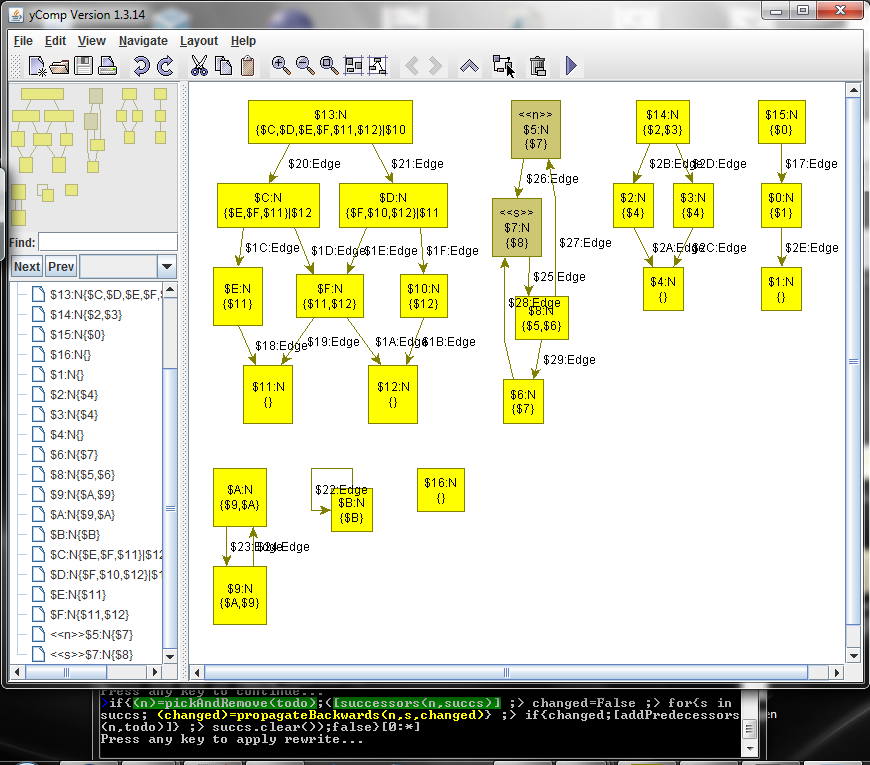
\includegraphics[width=\textwidth]{fig/Dataflow}
  \caption{Situation from dataflow analysis}
  \label{figdataflow}
\end{figure}

\subsubsection*{Worklist based data flow analysis}\indexmain{worklist}

The approach introduced above implements the basics but will not scale well to large graphs -- even medium sized graphs -- due to the random order the nodes are visited.
What is used in practice instead is a version employing a worklist built in postorder, so that a node is only visited after all its successor nodes have been processed.
For graphs without backedges, i.e. loops for program graphs, this gives an analysis which visits every node exactly once in the propagation phase.
For graphs with loops some nodes will be visited multiple times, but due to the ordering the analysis still terminates very fast.

The worklist is implemented directly in the graph by additional edges of the special type \verb#then# between the nodes, and a special node for the list start; the \verb#todo# set is kept, to allow for a fast "is the node already contained in the worklist"-check, used to save us from adding nodes again which are already contained (thus will be visited in the future anyway); i.e. the abstract worklist concept is implemented by the todo-set and the list added invasively to the graph.

  \begin{example}
    \begin{grgen}
edge class then; // for building worklist of nodes to be handled
    \end{grgen}
  \end{example}

\noindent The initial todo-set population of the simple approach is replaced by worklist constructing, successively advancing the last node of the worklist given by the \verb#last# variable; it starts with all nodes having no successor:\\
\verb#(last)=addFinalNodesToWorklist(last, todo)*#\\
Then iteratively all nodes which lead to them get added:\\
\verb#( (last)=addFurther(pos, last, todo)* ;> (pos)=switchToNextWorklistPosition(pos) )*#\\
In case of loops without terminal nodes we pick an arbitrary node from them:\\ \verb#(last)=addNotYetVisitedNodeToWorklist(last, todo)#\\
and add everything what leads to them, until every node was added to the worklist.

Now we can start the analysis, which works like the simple one does, utilizing the very same propagation rule,but follows the worklist instead of randomly picking from a todo-set, shrinking and growing the worklist along the way.

  \begin{example}
An example rule for worklist handling, adding a not yet contained node to the worklist; please note the quick check for containment via the set membership query.
    \begin{grgen}
rule addToWorklist(p:N, ref todo:set<N>, last:N) : (N)
{
  if{ !(p in todo); }

  modify {
    last -:then-> p;
    eval { todo.add(p); }
    return(p);
  }
}
    \end{grgen}
  \end{example}

  \begin{example}
An exmaple rule for worklist handling, removing the by-then processed node \texttt{pos} from the worklist.
    \begin{grgen}
rule nextWorklistPosition(pos:N, ref todo:set<N>) : (N)
{
  pos -t:then-> next:N;

  modify {
    delete(t);
    eval { todo.rem(pos); }
    return(next);
  }
}
    \end{grgen}
  \end{example}

The example can be found in the \texttt{tests/dataFlowAnalysis} directory, just add \texttt{debug} before the \texttt{xgrs} in \texttt{dataFlowAnalysisForReachabilityWorklist.grs} and watch it run.
A sample situation showing a worklist building step is given in \ref{figworklist}.
The subgraph at the top-left is already handled as you can see by the reachable set displayed in each node.

\begin{figure}[htbp]
  \centering
  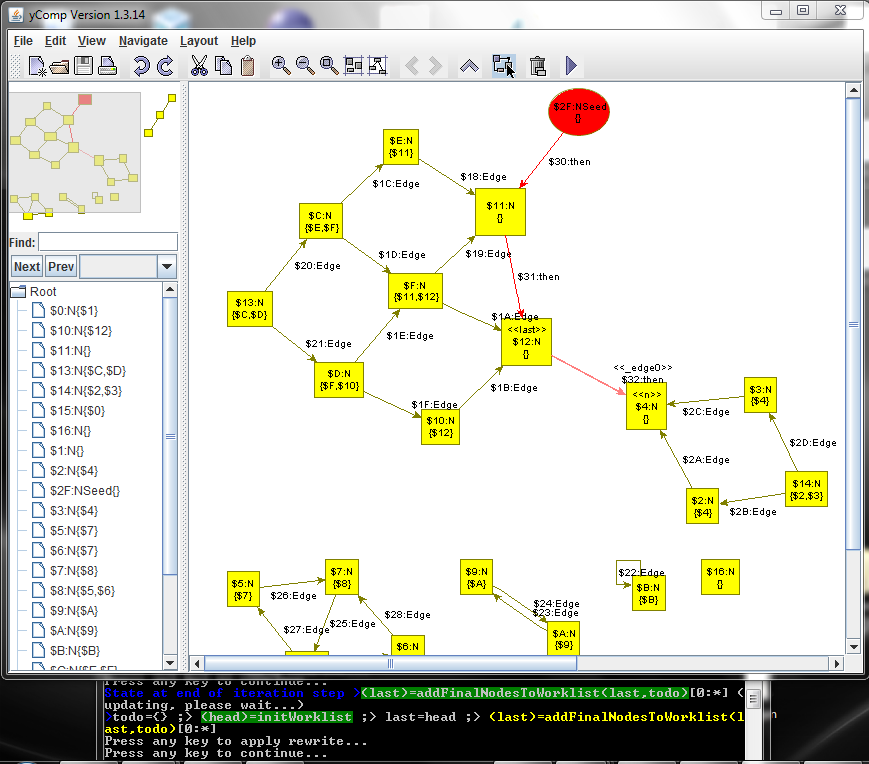
\includegraphics[width=\textwidth]{fig/Worklist}
  \caption{Situation from worklist building}
  \label{figworklist}
\end{figure}



\chapter{GrShell Language}\indexmain{GrShell}
\label{chapgrshell}
\GrShell\ is a \indexedsee{shell}{GrShell} application built on top of \LibGr\indexmain{libGr}. 
It belongs to \GrG's standard equipment. 
\GrShell\ is capable of creating, manipulating, and dumping graphs as well as performing and debugging graph rewriting.
The \GrShell\ provides a line oriented scripting language. 
\GrShell\ scripts are structured by simple statements separated by line breaks.

%rewrite stuff to be command based instead of splitting commands over several sections?

\section{Building Blocks}

\GrShell\ is \indexed{case sensitive}. 
A line may be empty, may contain a shell command, or may contain a comment. 
A \indexed{comment} starts with a \indexed{\texttt{\#}} and is terminated by end-of-line or end-of-file. 
The following items are required for representing text, numbers, and rule parameters.\\
\\
\emph{Text}\\
May be one of the following:
\begin{itemize}
  \item A non-empty character sequence consisting of letters, digits, and underscores. The first character must not be a digit.
  \item Arbitrary text enclosed by double quotes (\texttt{""}).
  \item Arbitrary text enclosed by single quotes (\texttt{''}).
\end{itemize}
\mbox{ }\\
\emph{Number}\\
Is an \texttt{int} or \texttt{float} constant in decimal notation (see also Section~\ref{sec:builtintypes}).

\begin{rail} 
 Parameters : Text + ',' ;
 SpacedParameters: Text + ; 
\end{rail}\ixnterm{Parameters}\ixnterm{SpacedParameters}

In order to describe the commands more precisely, the following (semantic) specializations of \emph{Text} are defined:
\begin{description}
  \item[Filename]A fully qualified file name without spaces (e.g.\ \texttt{/Users/Bob/amazing\textunderscore file.txt}) or a single quoted or double quoted fully qualified file name that may contain spaces (\texttt{"/Users/Bob/amazing file.txt"}).
  \item[Variable] Identifier of a (graph global) variable that contains a graph element or a value. \indexmainsee{GrShell variable}{graph global variable}
  \item[NodeType, EdgeType] Identifier of a node type resp.\ edge type defined in the model of the current graph.
  \item[AttributeName] Identifier of an attribute.
  \item[Graph] Identifies a graph by its name.
  \item[Action] Identifies a rule by its name.
  \item[Color] One of the following \indexed{color} identifiers: \texttt{Black}, \texttt{Blue}, \texttt{Green}, \texttt{Cyan}, \texttt{Red}, \texttt{Purple}, \texttt{Brown}, \texttt{Grey}, \texttt{LightGrey}, \texttt{LightBlue}, \texttt{LightGreen}, \texttt{LightCyan}, \texttt{LightRed}, \texttt{LightPurple}, \texttt{Yel\-low}, \texttt{White}, \texttt{DarkBlue}, \texttt{DarkRed}, \texttt{DarkGreen}, \texttt{DarkYellow}, \texttt{DarkMagenta}, \texttt{DarkCyan}, \texttt{Gold}, \texttt{Lilac}, \texttt{Turquoise}, \texttt{Aquamarine}, \texttt{Khaki}, \texttt{Pink}, \texttt{Orange}, \texttt{Orchid}. These are the same color identifiers as in \indexed{VCG}/\yComp\ files (for a VCG definition see~\cite{vcg}).
\end{description}
\makeatletter
\begin{rail}
  GraphElement: Text | ('@' '(' Text ')')
\end{rail}\indexmain{\texttt{"@}}\ixnterm{GraphElement}
\makeatother
The elements of a graph (nodes and edges) can be accessed both by their (graph global) \indexed{variable}\indexmain{graph global variable} identifier and by their \newterm{persistent name} specified through a constructor (see Section~\ref{mani}).
The specializations \emph{Node} and \emph{Edge} of \emph{GraphElement} require the corresponding graph element to be a node or an edge respectively.
\begin{example}
\label{persistentex} 
We insert a node, \indexed{anonymous}ly and with a \indexed{constructor} (see also Section~\ref{mani}):
\begin{grshell}
> new graph "../lib/lgsp-TuringModel.dll" G
New graph "G" of model "Turing" created.
  
# insert an anonymous node... 
# it will get a persistent pseudo name
> new :State  
New node "$0" of type "State" has been created.
> delete node @("$0")
  
# and now with constructor
> new v:State($=start) 
new node "start" of type "State" has been created.
# Now we have a node named "start" and a variable v assigned to "start"
\end{grshell}
\end{example}
\begin{note}
Persistent names will be saved (\texttt{save graph\dots}, see Section~\ref{outputcmds}) and exported, 
and, if you visualize a graph (\texttt{dump graph\dots}, see Section~\ref{outputcmds}), 
graph elements will be \indexed{label}ed with their persistent names.
Persistent names have to be unique for a graph (the graph they belong to).
\end{note}

\begin{rail}
  Variable '=' ( GraphElement | Variable | Literal )
\end{rail}
Assigns the variable or persistent name \emph{GraphElement} or literal to \emph{Variable}.
If \emph{Variable} has not been defined yet, it will be defined implicitly.
As usual for scripting languages, variables have neither static types nor declarations.
The variables known to \GrShell\ are the graph global variables (see \ref{cha:xgrs} for the distinction between graph global and sequence local variables).

\begin{rail} 
'show' 'var' Variable 
\end{rail}\ixkeyw{show}\ixkeyw{var}
Prints the content of the specified variable.


\section{\GrShell\ Commands}
This section describes the \GrShell\ commands\ixnterm{Command}. Commands are assembled from basic elements. 
As stated before commands are terminated by line breaks. Alternatively commands can be terminated by the \indexed{\texttt{;;}} symbol.
Like an operating system shell, the \GrShell\ allows you to span a single command over $n$ lines by terminating the first $n-1$ lines with a \indexed{backslash}.  
\begin{rail}
  Script: ((Command ('<line break>' | ';;'))+) '<end of file>' ;
\end{rail}\ixnterm{Script}


\subsection{Common Commands}
\label{commcommands}
\begin{rail}
  'help' (Command)?
\end{rail}\ixkeyw{help}
Displays an information message describing all the supported commands. 
A command \texttt{Command} displayed with \texttt{...} has further help available, which can be displayed with \texttt{help Command}.

\begin{rail}
  'quit' | 'exit'
\end{rail}\ixkeyw{quit}\ixkeyw{exit}
Quits \GrShell. If \GrShell\ is opened in debug mode, a currently active graph viewer (such as \yComp) will be closed as well.

\begin{rail}
  'include' Filename
\end{rail}\ixkeyw{include}
Executes the \GrShell\ script\indexmain{graph rewrite script} \emph{Filename}.
A \GrShell\ script is just a plain text file containing \GrShell\ commands.
They are treated as they would be entered interactively, except for parser error
If a parser error occurs, execution of the script will stop immediately.

\begin{rail}
  'echo' Text
\end{rail}\ixkeyw{echo}
Prints \emph{Text} onto the \GrShell\ command prompt.

\begin{rail}
  Variable '=' 'askfor' Type
\end{rail}\ixkeyw{askfor}
The \texttt{askfor} command interactively asks the user for a value of the specified type.
The entered value is type checked against the expected type, and assigned to the given variable in case it matches.
If the type is a value type, the user is prompted to enter a value literal with the keyboard.
If the type is a graph element type, the user is prompted to enter the graph element by double clicking in yComp.
Note that in this case the debug mode must have been enabled before.

\begin{example}
\begin{grshelllet}
x = askfor int
\end{grshelllet}
asks the user to enter an integer value; pressing 4 then 2 then enter will do fine.
\begin{grshelllet}
x = askfor Node
\end{grshelllet}
asks the user to select a graph element in yComp; double clicking any node will do fine. 
\end{example}

\begin{rail}
  '!' CommandLine
\end{rail}\indexmain{\texttt{"!}}
\emph{CommandLine}\indexmain{command line} is an arbitrary text, the operating system attempts to execute.
\begin{example}
On a Linux machine you might execute
\begin{grshell}
!sh -c "ls | grep stuff"
\end{grshell}
\end{example}

\begin{rail}
'silence' ('on'|'off')
\end{rail}\ixkeyw{silence}\ixkeyw{on}\ixkeyw{off}
Switches the new node / edge created / deleted messages on(default) or off.
Switching them off allows for much faster execution of scripts containing a lot of creation commands.

\begin{rail}
'randomseed' (Number | 'time')
\end{rail}\ixkeyw{randomseed}\ixkeyw{time}
Sets the random seed to the given number for reproducible results when using the \$-operator-prefix or the random-match-selector, whereas time sets the random seed to the current time in ms.

\begin{rail}
'redirect' 'emit' Filename
\end{rail}\ixkeyw{redirect}\ixkeyw{emit}
Redirects the output of the emit-statements in the rules from stdout to the given file.

\begin{rail}
'redirect' 'emit' '-'
\end{rail}\ixkeyw{redirect}\ixkeyw{emit}
Redirects the output of the emit-statements in the rules to stdout (again).


\subsection{Graph Commands}
\label{graphcommands}

\begin{rail}
  'new' 'graph' Filename Text 
\end{rail}\ixkeyw{new}\ixkeyw{graph}
Creates a new graph with the model specified in \emph{Filename}\indexmain{graph model}.
Its name is set to \emph{Text}. 
The model file can be either source code (e.g.\ \texttt{turing\textunderscore machineModel.cs}) or a .NET assembly (e.g.\ \texttt{lgsp-turing\textunderscore machineModel.dll}).
It's also possible to specify a rule set file as \emph{Filename}. 
In this case the necessary assemblies will be created on the fly.

\begin{rail}
  'open' 'graph' Filename Text
\end{rail}\ixkeyw{open}\ixkeyw{graph}
Opens the graph \emph{Text} stored in the backend. 
However, the \emph{LGSPBackend} doesn't support \indexed{persistent graph}s, and as the \emph{LGSPBackend} is the only backend available at the moment, this command is currently useless.
You may achieve persistence by using import/export or save/include instead.

\begin{rail}
  'show' 'graphs'
\end{rail}\ixkeyw{show}\ixkeyw{graph}
Displays a list of currently available graphs.

\begin{rail}
  'select' 'graph' Graph
\end{rail}\ixkeyw{select}\ixkeyw{graph}
Selects the current \indexed{working graph}.
This graph acts as \emph{\indexed{host graph}} for graph rewrite sequences (see also Sections~\ref{ov:whatsallabout} and~\ref{grsthings}).
Though you can define multiple graphs, only one graph can be the active ``working graph''.

\begin{rail}
  'clear' 'graph' (() | Graph)
\end{rail}\ixkeyw{clear}\ixkeyw{graph}
Deletes all graph elements of the current working graph resp.\ the graph \emph{Graph}.

\begin{rail}
  'delete' 'graph' Graph
\end{rail}\ixkeyw{delete}\ixkeyw{graph}
Deletes the graph \emph{Graph} from the backend storage.


\subsection{Validation Commands}

\GrG\ offers two different graph validation mechanisms, the first checks against the connection assertions specified in the model, the second checks against an arbitrary graph rewrite sequence containing arbitrary tests and rules.

\begin{rail}
  'validate' ('exitonfailure')? ('strict')?
\end{rail}\ixkeyw{validate}\ixkeyw{exitonfailure}\ixkeyw{strict}
Validates\indexmain{validate} if the current working graph fulfills the \indexed{connection assertion}s specified in the corresponding graph model.
The \emph{strict} mode additionally requires all the edges available in the instance graph to be specified in the model in order to be ``valid''.
Otherwise edges between nodes without specified constraints are ignored.

\begin{rail}
  'validate' ('exitonfailure')? 'xgrs' GRS
\end{rail}\ixkeyw{validate}\ixkeyw{exitonfailure}\ixkeyw{xgrs}
Validates\indexmain{validate} if the current working graph satisfies the \indexed{graph rewrite sequence} given.
Before the graph rewrite sequence is executed, the instance graph gets cloned;
the sequence operates on the clone, allowing you to change the graph as you want to, without influence on the host graph.
Validation fails iff the xgrs fails.
This gives a rather costly but extremely flexible and powerful mechanism to specify graph constraints.
The GrShell is exited with an error code if \texttt{exitonfailure} is specified and the validation fails.

\begin{example}
We reuse a simplified version of the road map model from Chapter~\ref{chapmodellang}:
\begin{grgen} 
model Map;

node class city;
node class metropolis;

edge class street;
edge class highway
      connect metropolis [+] -> metropolis [+];
\end{grgen}
The node constraint on \emph{highway} requires all the metropolises to be connected by highways. Now have a look at the following graph:
\begin{center}
  \fbox{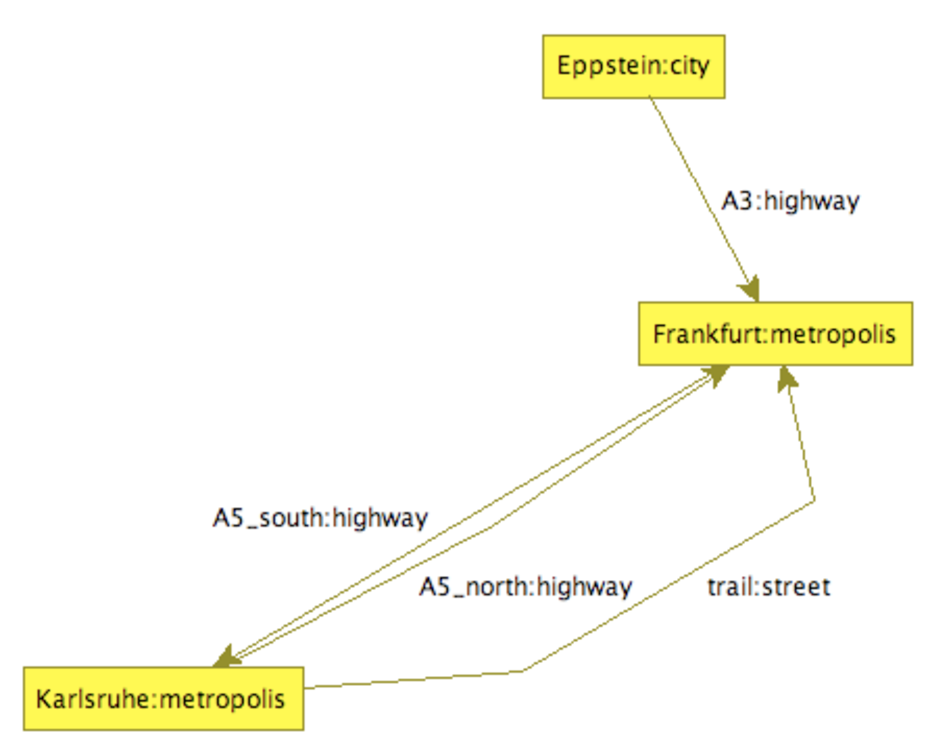
\includegraphics[width=8.5cm]{fig/map}}
\end{center}

This graph is valid but not strict valid.
\begin{grshell} 
> validate
The graph is valid.
> validate strict
The graph is NOT valid:
  CAE: city "Eppstein" -- highway "A3" --> metropolis "Frankfurt" not specified
  CAE: metropolis "Karlsruhe" -- street "trail" --> metropolis "Frankfurt" not specified
>
\end{grshell}
\end{example}


\pagebreak

\subsection{Graph Input and Output Commands}
\label{outputcmds}

\begin{rail}
  'save' 'graph' Filename
\end{rail}\ixkeyw{save}\ixkeyw{graph}
Dumps\indexmain{dumping graph} the current graph as \GrShell\ script\indexmain{graph rewrite script} into \emph{Filename}.
The created script includes
\begin{itemize}
  \item selecting the backend
  \item creating a new graph with all nodes and edges (including their persistent names)
  \item restoring the (graph global) variables
  \item restoring the visualisation styles
\end{itemize}
but not necessarily using the same commands you typed in during construction. 
Such a script can be loaded and executed by the \texttt{include} command (see Section~\ref{commcommands}).

\begin{rail}
  'export' Filename ('.grs' | '.grsi') ('.gz')? ('withvariables')?
\end{rail}\ixkeyw{export}\ixkeyw{withvariables}\indexmain{export}
Exports an instance graph in GRS (.grs/.grsi) format, which is a reduced \GrShell\ script
(it can get imported and exported on API level\ref{sub:imexport} without using the \GrShell).
It contains the \texttt{new graph} command, followed by \texttt{new node} commands, followed by \texttt{new edge} commands.
If the \texttt{.gz} suffix is given the graph is saved zipped.
If \texttt{withvariables} is specified, the (graph global) variables are exported, too.
The export is only complete with the model of the graph given in the \texttt{.gm} file.
Exporting fails if the graph model contains attributes of \texttt{object}-type.
The \texttt{save} command is for saving about a \GrShell\ session including graph global variables and visualization commands, 
the goal of the \texttt{export} command is basic graph rewrite system interoperability.
The persistent names are saved in contrast to the following format GXL.

\begin{rail}
  'export' Filename '.gxl' ('.gz')?
\end{rail}\ixkeyw{export}\indexmain{import}
Exports an instance graph and a graph model in GXL format \cite{GXL,GXL2}, 
which is somewhat of a standard format for graphs of graph rewrite systems, 
but suffers from the well-known XML problems -- it is barely human-readable and bloated.
Exporting fails if the graph model contains attributes of \texttt{set<S>}-,\texttt{map<S,T>}-, or \texttt{object}-type.
If the \texttt{.gz} suffix is given the graph is saved zipped.

\begin{rail}
  'import' Filename ('.grs' | '.grsi' ) ('.gz')?
\end{rail}\ixkeyw{import}
Imports the specified graph instance in GRS (.grs/.grsi) format (the \emph{reduced} \GrShell\ script,
a saved graph can only be imported by \texttt{include} (but an exported graph can be imported by \texttt{include}, too)).
The referenced graph model must be available as \texttt{.gm}-file.
If the \texttt{.gz} suffix is given the graph is expected to be zipped.

\begin{rail}
  'import' Filename '.gxl' ('.gz')? (ModelOverride)?
\end{rail}\ixkeyw{import}
Imports the specified graph instance and model in GXL format.
If a model override of the form \texttt{Filename.gm} is specified, the given model will be used instead of the model in the GXL file.
The \texttt{.gxl}-graph must be compatible to the \texttt{.gm}-model.
If the \texttt{.gz} suffix is given the graph is expected to be zipped.

\begin{note}\label{shellgxlimport}
Normally you are not only interested in importing a GXL graph (and viewing it), but you want to execute actions on it.
The problem is that the actions are model dependent.
So, in order to apply actions, you must use a model override, which works this way:
\begin{enumerate}
\item \texttt{new graph "YourName.grg"}\\
This creates the model library lgsp-YourNameModel.dll
and the actions library lgsp-YourNameActions.dll
(which depends on the model library generated from the \texttt{"using YourName;"}).
\item \texttt{import InstanceGraphOnly.gxl YourName.gm}\\
This imports the instance graph from the .gxl but uses the model specified
in YourName.gm (it must fit to the model in the .gxl in order to work).
\item \texttt{select actions lgsp-YourNameActions.dll}\\
This loads the actions from the actions library in addition to the already
loaded model and instance graph (cf. \ref{grsthings}).
\item Now you are ready to use the actions.
\end{enumerate}
\end{note}

\begin{note}\label{shellecoreexport}
Further formats available for import are \texttt{.ecore} plus \texttt{.xmi}.
These are formats common to the model transformation community which are not directly geared towards graphs, so they can't be imported directly.
Instead during the import process an intermediate \texttt{.gm} is written which is equivalent to the \texttt{.ecore} given -- you may inspect it to see how the content gets mapped
(the importer maps classes to GrGen node classes, their attributes
to corresponding GrGen attributes, and their references to GrGen
edge classes; inheritance is transferred one-to-one, and enumerations are
mapped to GrGen enums; class names are prefixed by the names of the
packages they are contained in to prevent name clashes).
After this metamodel transformation the instance graph XMI adhering to the Ecore model thus adhering to the just
generated equivalent GrGen graph model gets imported.
Furthermore you can give specify a \texttt{.grg} containing the rules to apply (using further rule and model files).
The importer was added for a GraBaTs challenge and is available as-is -- it may or may not work for you, 
if you need more it's on you to improve it. An export is not available -- we coded the export we needed with emit statements.
\begin{rail}
  'import' ((Filename '.ecore')+( )) Filename '.xmi' (Filename '.grg')?
\end{rail}\ixkeyw{import}
\end{note}

\begin{rail}
  'import' 'add' FileSpec 'withvariables'
\end{rail}\ixkeyw{import}\ixkeyw{add}
Imports the graph in the specified file and adds it to the current graph
(instead of overwriting the old graph with the new graph).
The \texttt{FileSpec} is of the same format as the file specification in the other two imports.
The \texttt{withvariables} argument only yields an effect if the file to import contains variable specifications (the content of old variables of the same name is overwritten).


\subsection{Graph Manipulation Commands}
\label{mani}
Graph manipulation commands alter existing graphs; they allow to create and delete graph elements and change attributes. 
These are tasks which should be carried by the rules of the rule language -- the commands are mainly used as elementary instructions in graph input and output.

\begin{rail}
  'new' (() | Text) (() | ':' NodeType (() | Constructor))
\end{rail}\ixkeyw{new}
Creates a new node within the current graph.
Optionally a variable \emph{Text} is assigned to the new node.
If \emph{NodeType} is supplied, the new node will be of type \emph{NodeType} and attributes can be initialized by a constructor.
Otherwise the node will be of the base node class type \emph{Node}.
\begin{note}
The \GrShell\ can reassign \indexed{variable}s. 
This is in contrast to the rule language (Chapter~\ref{chaprulelang}), where we use \emph{names}\indexmain{name}\indexmain{expression variable}\indexmainsee{expression variable}{name}.
\end{note}

\begin{rail}
  'new' Node (('-' EdgeEntityConstructor '->') | ('-' EdgeEntityConstructor '-')) Node ;
EdgeEntityConstructor:
  (()|Text) (() | ':' EdgeType (() | Constructor)) ;
\end{rail}\ixkeyw{new}
Creates a new edge within the current graph between the specified nodes,
directed from the first to the second \emph{Node} in the case of \texttt{-->},
or undirected in the case of \texttt{--}.
Optionally a variable \emph{Text} is assigned to the new edge.
If \emph{EdgeType} is supplied, the new edge will be of type \emph{EdgeType} and attributes can be initialized by a constructor.
Otherwise the edge will be of the base edge class type \texttt{Edge} for \texttt{-->} or \texttt{UEdge} for \texttt{--}.

\begin{rail}
  Constructor : '(' (() | (dollar '=' Text (() | ',' Attributes) | Attributes)) ')';
  Attributes : (AttributeName '=' AttributeValue) + (',');
  AttributeValue :  PrimitiveAttributeValue | SetConstr | MapConstr ;
  PrimitiveAttributeValue : EnumLit | Number | DoubleNum | FloatNum | QuotedText | BoolLit | NullLit ;
  SetConstr: 'set' '<' Type '>' lbrace ( Expression*',' ) rbrace ;
  MapConstr: 'map' '<' Type ',' Type '>' \\ lbrace ( (Expression '->' Expression)*',' ) rbrace ;
\end{rail}\indexmain{\texttt{\$}}\ixnterm{Constructor}\ixnterm{Attributes}\ixnterm{AttributeValue}\ixnterm{PrimitiveAttributeValue}\ixnterm{SetConstr}\ixnterm{MapConst}
A \indexed{constructor} is used to initialize a new graph element (see \texttt{new \dots} below).
A comma separated list of \indexed{attribute} declarations is supplied to the constructor.
Available attribute names are specified by the graph model of the current working graph.
All the undeclared attributes will be initialized with \indexed{default value}s, depending on their type 
(\texttt{int} $\leftarrow$ \texttt{0}; \texttt{boolean} $\leftarrow$ \texttt{false}; \texttt{float} $\leftarrow$ \texttt{0.0f}; \texttt{double} $\leftarrow$ \texttt{0.0}; \texttt{string} $\leftarrow$ \texttt{""}; \texttt{set<T>} $\leftarrow$ \texttt{set<T>\{\}}; \texttt{map<S,T>} $\leftarrow$ \texttt{map<S,T>\{\}}; \texttt{enum} $\leftarrow$ unspecified;).\\
The \texttt{\$} is a special attribute name: a unique identifier of the new graph element.
This identifier is also called \newterm{persistent name} (see Example~\ref{persistentex}).
This name can be specified by a constructor only.

\begin{rail}
  'delete' 'node' Node
\end{rail}\ixkeyw{delete}\ixkeyw{node}
Deletes the node \emph{Node} from the current graph.
Incident edges will be deleted as well.

\begin{rail}
  'delete' 'edge' Edge
\end{rail}\ixkeyw{delete}\ixkeyw{edge}
Deletes the edge \emph{Edge} from the current graph.

\begin{rail}
  GraphElement '.' AttributeName '=' (Text | Number) ;
\end{rail}
Set the \indexed{attribute} \emph{AttributeName} of the graph element \emph{GraphElement} to the value of \emph{Text} or \emph{Number}.

  
\subsection{Graph and Model Query Commands}

\begin{rail}
  'show' (() | 'num') ('nodes' (() | (() | 'only') NodeType) | 'edges' (() | (() | 'only') EdgeType))
\end{rail}\ixkeyw{show}\ixkeyw{num}\ixkeyw{nodes}\ixkeyw{edges}\ixkeyw{only}
Gets the \indexed{persistent name}s and the types of all the nodes/edges of the current graph. 
If a node type or edge type is supplied, only elements compatible to this type are considered. 
The \texttt{only} keyword excludes subtypes. Nodes/edges without persistent names are shown with a pseudo-name.
If the command is specified with \texttt{num}, only the number of nodes/edges will be displayed.

\begin{rail}
  'show' ('node' | 'edge') 'types'
\end{rail}\ixkeyw{show}\ixkeyw{node}\ixkeyw{edge}\ixkeyw{types}
Gets the node/edge types of the current graph model.

\begin{rail}
'show' ('node' ('super' | 'sub') 'types' NodeType | 'edge' ('super' | 'sub') 'types' EdgeType)
\end{rail}\ixkeyw{show}\ixkeyw{node}\ixkeyw{edge}\ixkeyw{super}\ixkeyw{sub}\ixkeyw{types}\indexmain{inheritance}
Gets the inherited/descendant types of \emph{NodeType}/\emph{EdgeType}.

\begin{rail}
  'show' ('node' 'attributes' (() | (() | 'only') NodeType) | 'edge' 'attributes' (() | (() | 'only') EdgeType))
\end{rail}\ixkeyw{show}\ixkeyw{node}\ixkeyw{edge}\ixkeyw{only}\ixkeyw{attributes}
Gets the available node/edge \indexed{attribute} types.
If \emph{NodeType}/\emph{EdgeType} is supplied, only attributes defined in \emph{NodeType}/\emph{EdgeType} are diplayed.
The \texttt{only} keyword excludes inherited attributes.\\
\begin{note}
The \texttt{show nodes/edges attributes\dots} command covers types and \emph{inherited} types.
This is in contrast to the other \texttt{show\dots} commands where types and \emph{sub}types are specified or the direction in the type hierarchy is specified explicitly, respectively.
\end{note}

\begin{rail}
 'show' ('node' Node | 'edge' Edge)
\end{rail}\ixkeyw{show}\ixkeyw{node}\ixkeyw{edge}
Gets the attribute types and values of a specific graph element.

\begin{rail}
  'show' GraphElement '.' AttributeName
\end{rail}\ixkeyw{show}
Displays the value of the specified attribute.

\begin{rail}
  'node' 'type' Node 'is' Node | 'edge' 'type' Edge 'is' Edge
\end{rail}\ixkeyw{node}\ixkeyw{edge}\ixkeyw{type}\ixkeyw{is}
Gets the information whether the first element is \indexed{type-compatible}\indexmainsee{compatible types}{type-compatible} to the second element.


\subsection{Graph Visualization Commands}\label{sub:visual}\indexmain{visualization}\indexmainsee{layout}{visualization}\indexmainsee{visualization}{group node}

\begin{rail}
  'show' 'graph' ExecutableName (() | Text)
\end{rail}\ixkeyw{show}\ixkeyw{graph}
Dumps the current graph in \indexed{VCG} format into a temporary file.
The temporary VCG file will be passed to the program \emph{ExecutableName} as first parameter;
further parameters, such as program options, can be specified by \emph{Text}.
If you use \yComp\footnote{See Section~\ref{tools:ycomp}.}\indexmain{yComp} as executable (\texttt{show graph ycomp}), this may look like
\begin{center}
  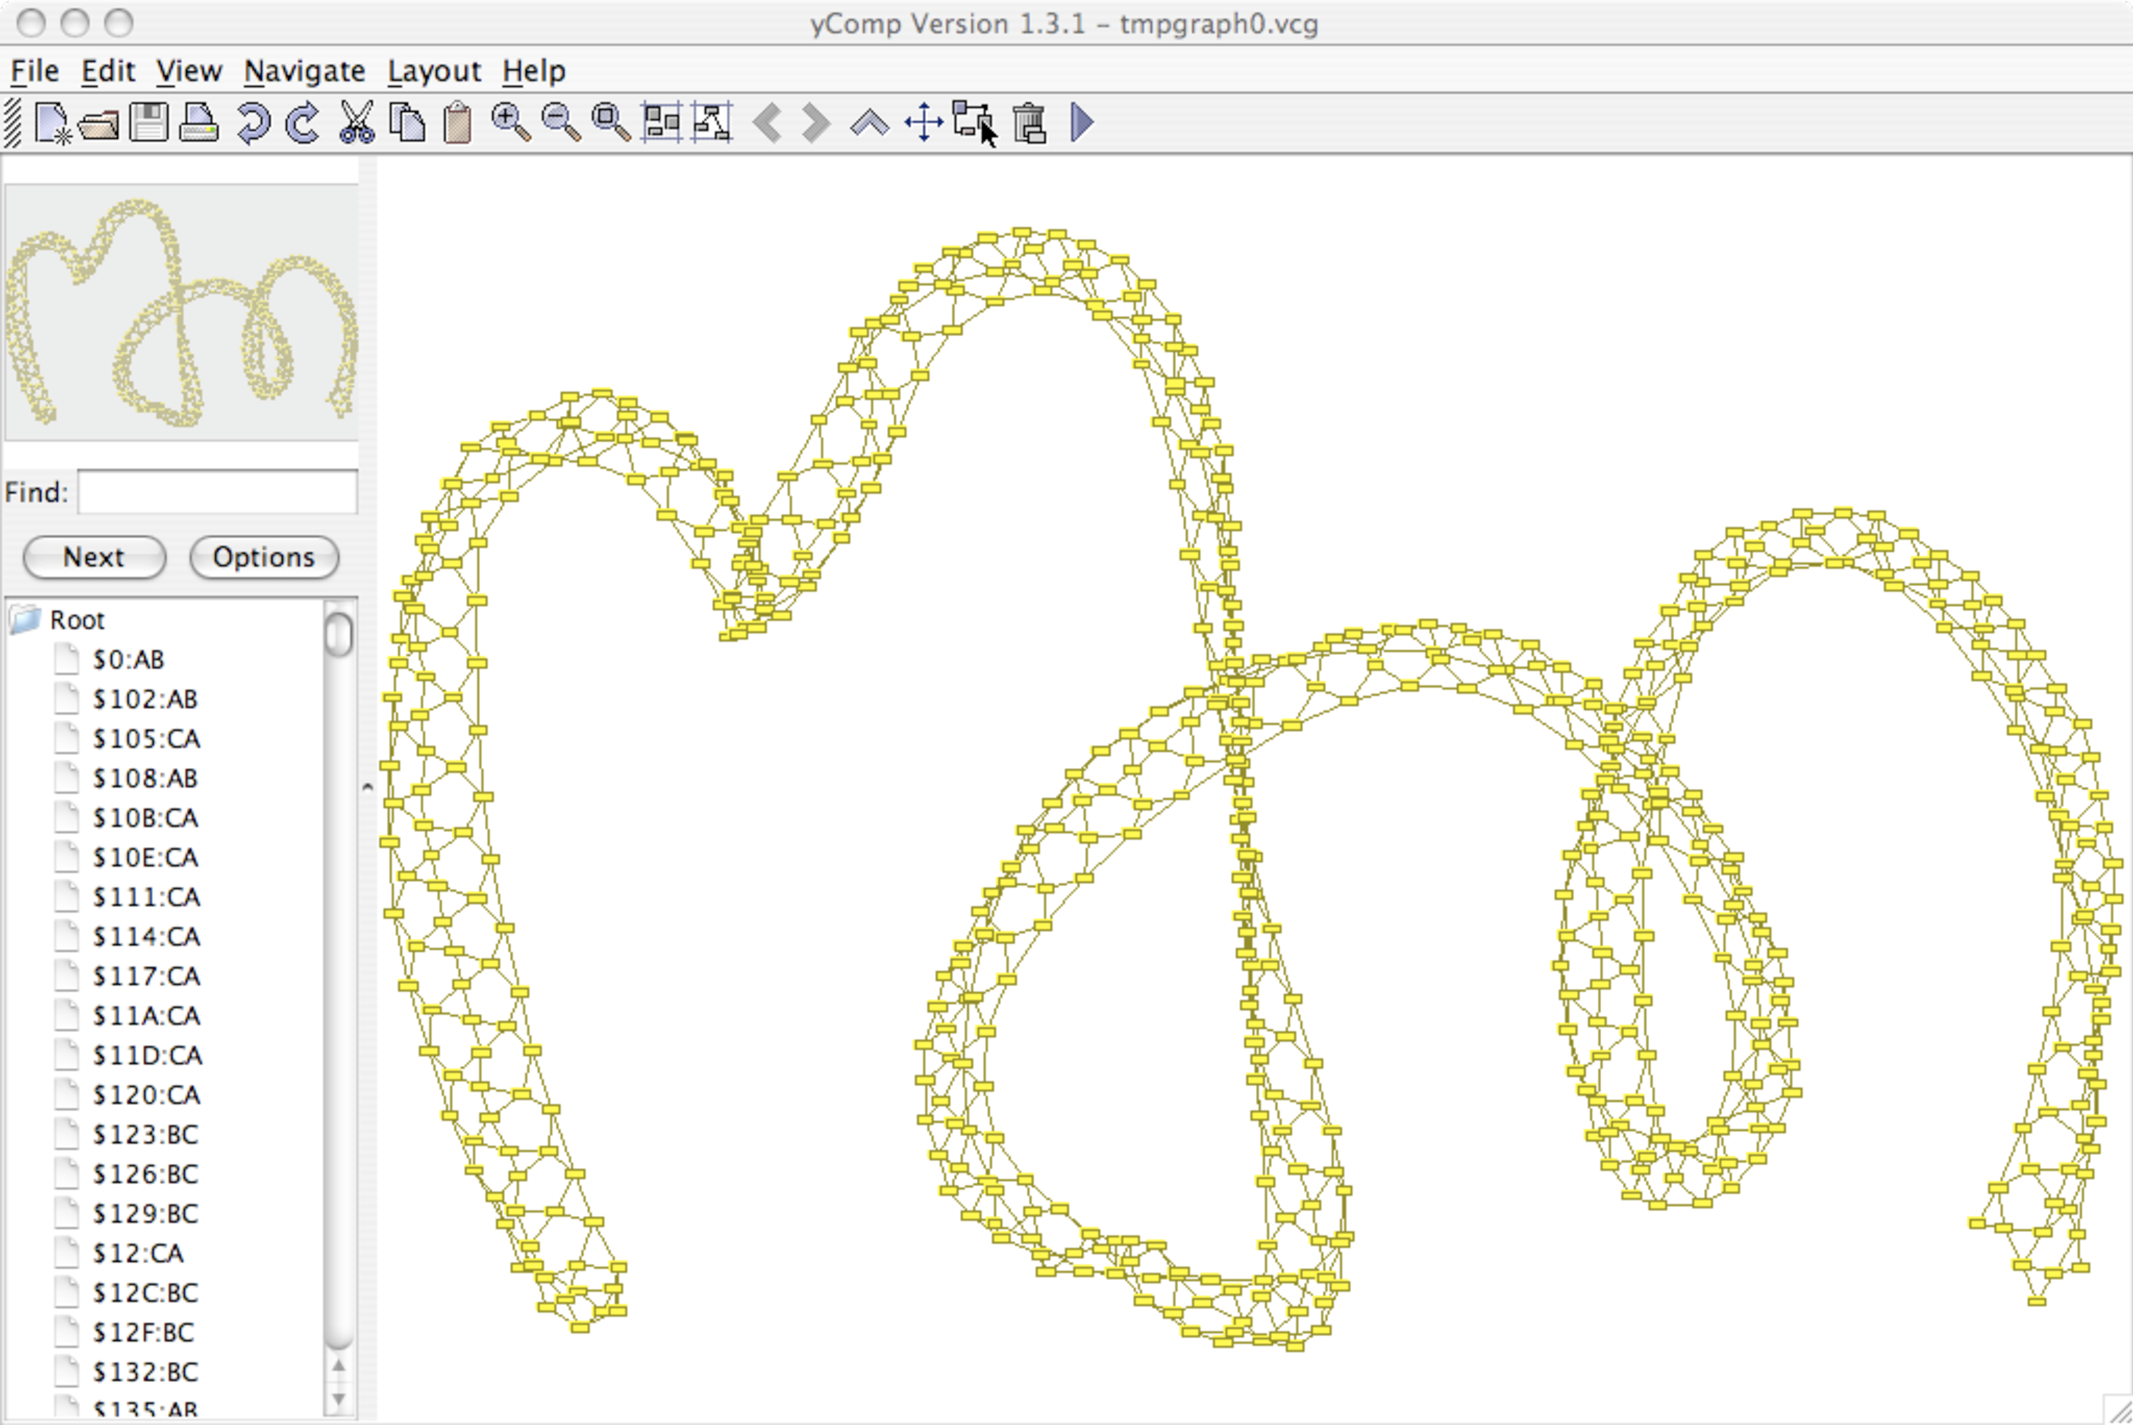
\includegraphics[width=0.75\linewidth]{fig/showgraph}
\end{center}  
The temporary file will be deleted, when the application \emph{Filename} is terminated if \GrShell\ is still running at this time.

\begin{rail}
  'dump' 'graph' Filename
\end{rail}\ixkeyw{dump}\ixkeyw{graph}
Dumps the current graph in \indexed{VCG} format into the file \emph{Filename}.\\

The following commands control the style of the VCG output. This affects \texttt{dump graph}, \texttt{show graph}, and \texttt{enable debug}. 
\begin{rail}
  'dump' 'set' 'node' (() | 'only') NodeType \\ (('color' | 'textcolor' | 'bordercolor') Color | 'shape' Text | 'labels' ('on' | 'off' | Text)) ;
\end{rail}\ixkeyw{dump}\ixkeyw{set}\ixkeyw{node}\ixkeyw{only}\ixkeyw{color}\ixkeyw{textcolor}\ixkeyw{bordercolor}\ixkeyw{shape}\ixkeyw{labels}\ixkeyw{on}\ixkeyw{off}
Sets the \indexed{color}, text color, border color, the shape or the label of the nodes of type \emph{NodeType} and all of its subtypes.
The keyword \texttt{only} excludes the subtypes. The available colors are specified at the begin of this chapter. 
The following shapes are supported: \texttt{box}, \texttt{triangle}, \texttt{circle}, \texttt{ellipse}, \texttt{rhomb}, \texttt{hexagon}, \texttt{trapeze}, \texttt{uptrapeze}, \texttt{lparallelogram}, \texttt{rparallelogram}.
Those are shape names of \yComp\ (for a VCG definition see~\cite{vcg}).
The default labeling is set to \texttt{on} with \texttt{Name:Type}, it can be overwritten by an specified label string (e.g. the source code line originating the node in a program graph) or switched off.

\begin{rail}
  'dump' 'set' 'edge' (() | 'only') EdgeType \\ (('color' | 'textcolor') Color | 'labels' ('on' | 'off' | Text));
\end{rail}\ixkeyw{dump}\ixkeyw{set}\ixkeyw{edge}\ixkeyw{only}\ixkeyw{color}\ixkeyw{textcolor}\ixkeyw{labels}\ixkeyw{on}\ixkeyw{off}
Sets the color, text color or label of the edges of type \emph{EdgeType} and all of its subtypes.
The keyword \texttt{only} excludes the subtypes. The available colors are specified at the begin of this chapter.
The default labeling is set to \texttt{on} with \texttt{Name:Type}, it can be overwritten by an specified label string or switched off.

\begin{rail}
  'dump' 'add' (('node' ('only')? NodeType)|('edge' ('only')? EdgeType)) 'exclude' ;
\end{rail}\ixkeyw{dump}\ixkeyw{add}\ixkeyw{node}\ixkeyw{edge}\ixkeyw{only}\ixkeyw{exclude}
Excludes nodes/edges of type \emph{NodeType}/\emph{EdgeType} and all of its subtypes from output, for a node it also excludes its incident edges.
The keyword \texttt{only} excludes the subtypes from exlusion, i.e.\ subtypes of \emph{NodeType}/\emph{EdgeType} are dumped.

\begin{rail}
  'dump' 'add' 'node' ('only')? NodeType 'group' (GroupConstraints)? ;
GroupConstraints:
  'by' ('hidden')? GroupMode (IncAdjTypeConstraints)? ;
IncAdjTypeConstraints:
  ('only')? EdgeType ('with' ('only')? NodeType)? ;
\end{rail}\ixkeyw{dump}\ixkeyw{add}\ixkeyw{node}\ixkeyw{only}\ixkeyw{group}\ixkeyw{by}\ixkeyw{hidden}\ixkeyw{with}\ixnterm{GroupConstraints}\ixnterm{IncAdjTypeConstraints}
Declares \emph{NodeType} and subtypes of \emph{NodeType} as \indexed{group node}\indexmainsee{hierarchic}{group node} type.
All the differently typed nodes that point to a node of type \emph{NodeType} 
(i.e.\ there is a directed edge between such nodes) will be grouped and visibly enclosed by the \emph{NodeType}-node.
\texttt{GroupMode} is one of \texttt{no},\texttt{incoming},\texttt{outgoing},\texttt{any}; \texttt{hidden} causes hiding of the edges by which grouping happens.
The \texttt{EdgeType} constrains the type of the edges which cause grouping, the \texttt{with} clause additionally constrains the type of the adjacent node; 
\texttt{only} excludes subtypes.

\begin{note}
Only apply group commands on a graph if they indeed lead to a containment tree of groups.
If the group commands would lead to a directed acyclic or even cyclic containment graph, the results are undefined.
You may get duplicate edges (and nodes); the implementation is free to choose indeterministically between the possible nestings -- it may even grow an arm and stab you in your back.
(A conflict resultion heuristic used is to give the earlier executed \texttt{add group} command priority. 
But this mechanism is incomplete -- you'd better refine your groups or change the model in that case.
Using a model separating edges denoting direct containment from cross-linking edges by type is normally the better design, even disregarding visual node nesting.)
\end{note}

The following example shows \emph{metropolis} ungrouped and grouped:
\begin{center}
  \fbox{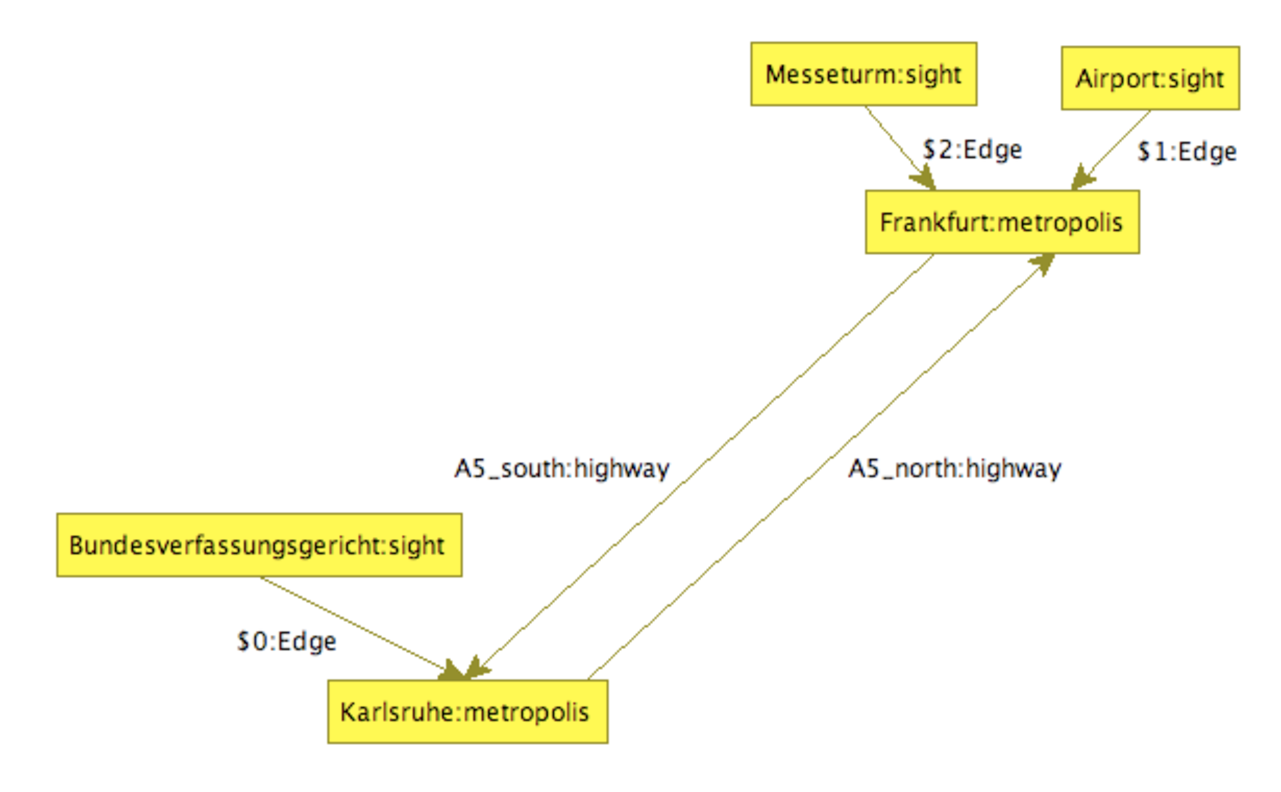
\includegraphics[width=0.45\linewidth]{fig/group2-1}}  \hfill \fbox{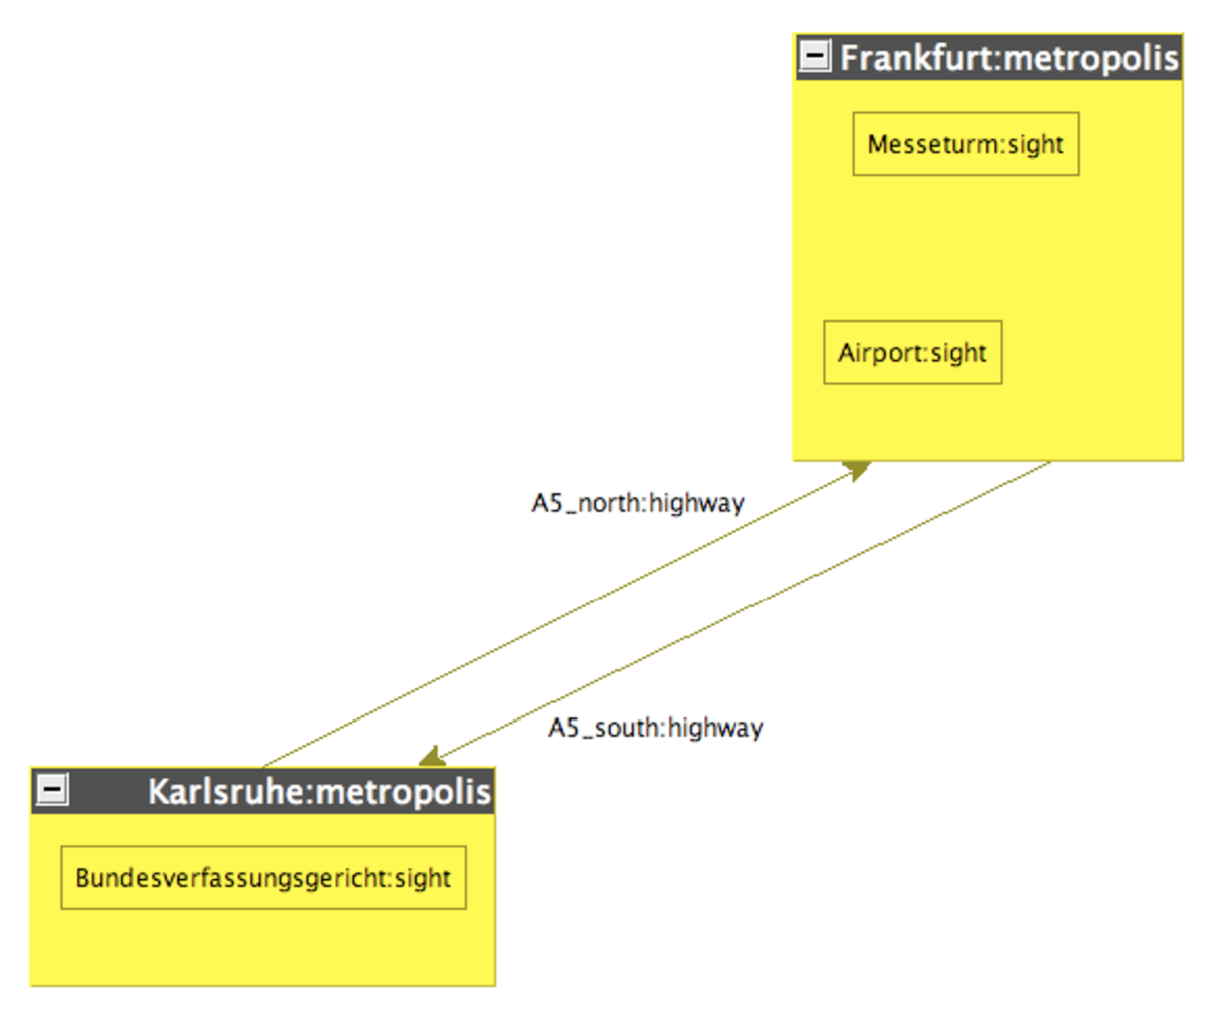
\includegraphics[width=0.45\linewidth]{fig/group2-2}}\\
  {\small right side: dumped with \texttt{dump add node metropolis group}}
\end{center}

\begin{rail}
  'dump' 'add' (() | 'only') ('node' NodeType | 'edge' EdgeType) \\ ('infotag' | 'shortinfotag') AttributeName
\end{rail}\ixkeyw{dump}\ixkeyw{add}\ixkeyw{only}\ixkeyw{node}\ixkeyw{edge}\ixkeyw{infotag}\ixkeyw{shortinfotag}
Declares the \indexed{attribute} \emph{AttributeName} to be an ``\indexed{info tag}'' or ``\indexed{short info tag}''.
Info tags are displayed like additional node/edge \indexed{label}s, in format \texttt{Name=Value}, or \texttt{Value} only for short info tags. 
The keyword \texttt{only} excludes the subtypes of \emph{NodeType} resp.\ \emph{EdgeType}. 
In the following example \emph{river} and \emph{jam} are info tags:
\begin{center}
  \fbox{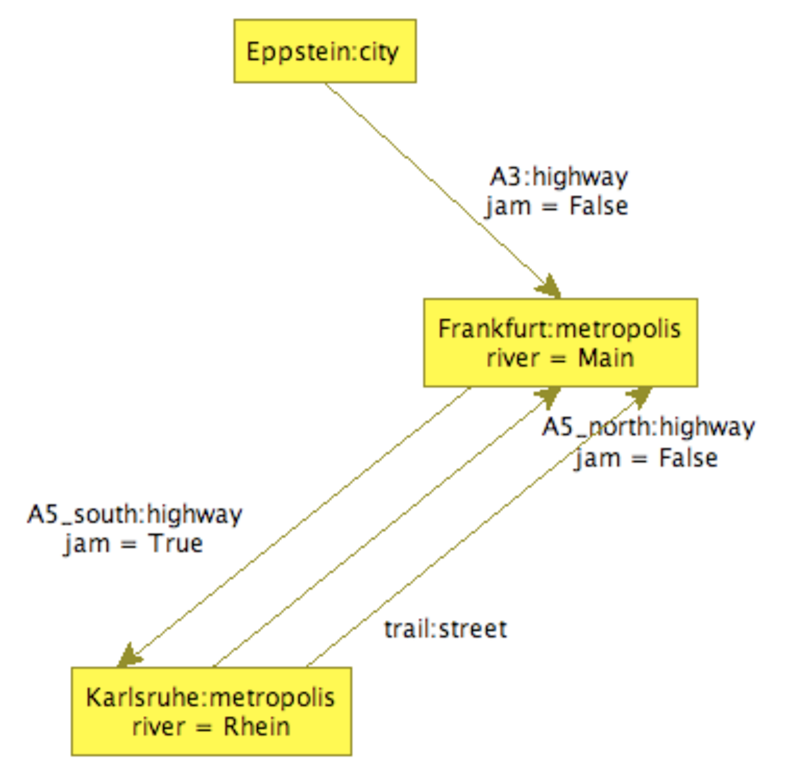
\includegraphics[width=0.5\linewidth]{fig/infotag}}
\end{center}

\begin{rail}
  'dump' 'reset'
\end{rail}\ixkeyw{dump}\ixkeyw{reset}
Resets all style options (\texttt{dump set}\dots) and (\texttt{dump add}\dots) to their default values.


\begin{note}\label{note:visual}
Small graphs allow for fast visual understanding, but with an increasing number of nodes and edges they quickly loose this property.
The group commands are of outstanding importance to keep readability with increasing graph sizes
(e.g. for program graphs it allows to lump together expressions of a method inside the method node and attributes of the class inside the class node).
Additional helpers in keeping the graph readable are: 
the capability to exclude elements from dumping (the less hay in the stack the easier to find the needle),
the different colors and shapes to quickly find the elements of interest,
as well as the labels/infotags/shortinfotags to display the most important information directly. 
Choose the layout algorithm and the options delivering the best results for your needs, organic and hierarchic or compiler graph 
(an extension of hierarchic with automatic edge cutting -- marking cut edges by fat dots, showing the edge only on mouse over and allowing to jump to the other end on a mouse click)
should be tried first.
\end{note}

The following example shows several of the layout options employed to considerably increase the readability of a program graph (as given in \texttt{examples/JavaProgramGraphs-GraBaTs08}):
\begin{center}
  \fbox{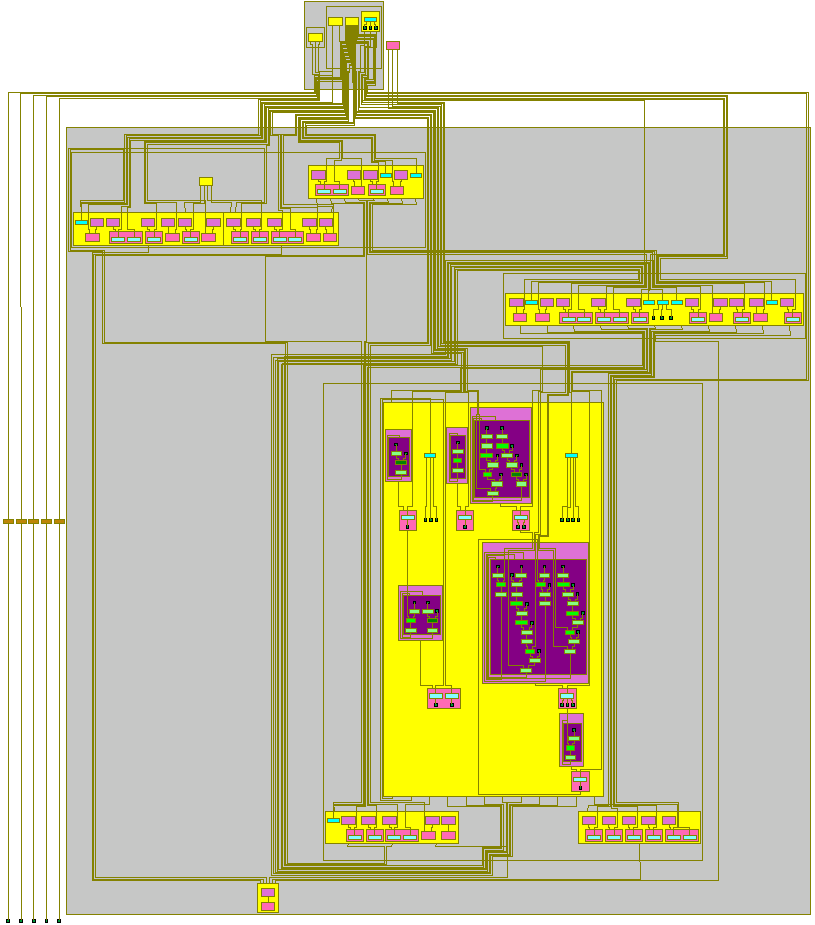
\includegraphics[width=0.45\linewidth]{fig/screen-overview}}  \hfill \fbox{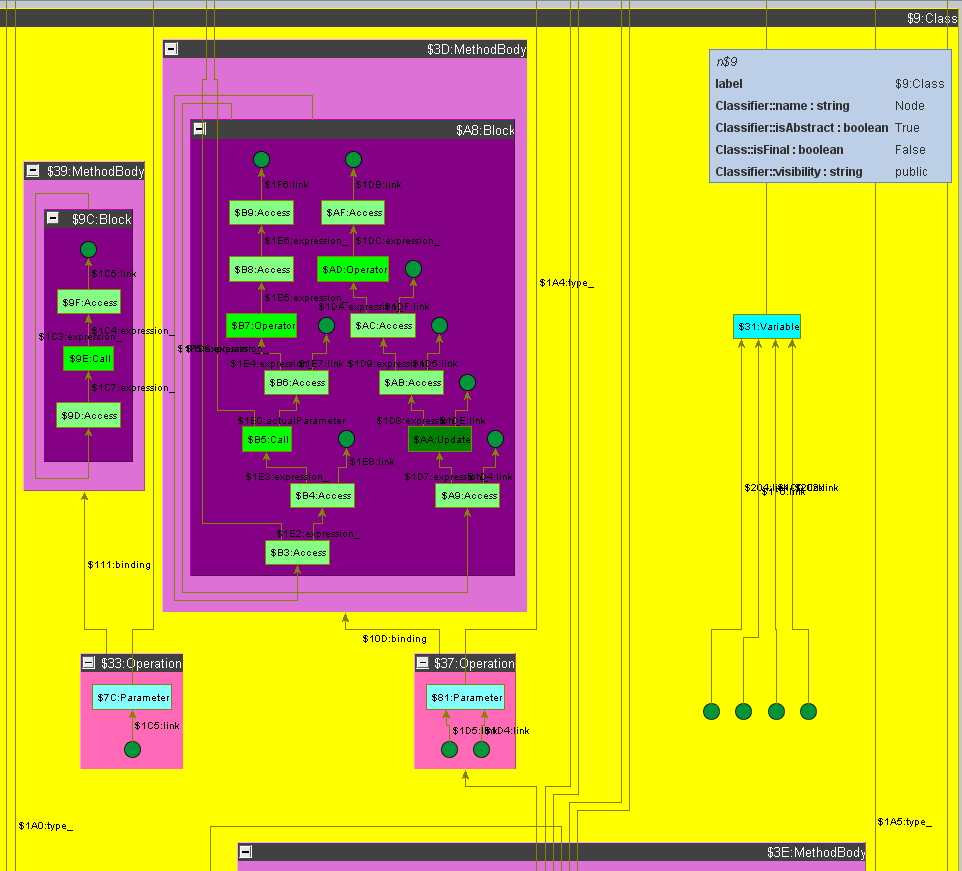
\includegraphics[width=0.45\linewidth]{fig/screen-detail}}\\
  {\small Overview of the initial program graph and some details of the ``Node'' class}
\end{center}


\subsection{Action Commands (XGRS)}\indexmain{action command}\indexmainsee{action}{graph rewrite sequence}
\label{grsthings}
An \emph{action} denotes a graph rewrite rule.

\begin{rail}
  'select' 'actions' Filename
\end{rail}\ixkeyw{select}\ixkeyw{actions}
Selects a \indexed{rule set}.
\emph{Filename} can either be a .NET assembly (e.g.\ ``rules.dll'') or a source file (``rules.cs'').
Only one rule set can be loaded simultaneously.

\begin{rail}
  'show' 'actions'
\end{rail}\ixkeyw{show}\ixkeyw{actions}
Lists all the rules of the loaded rule set, their parameters, and their return values.
Rules can return a set of graph elements.

\begin{rail}
  'custom' 'actions' (() | SpacedParameters)
\end{rail}\ixkeyw{custom}\ixkeyw{actions}
Executes an action specific to the current \indexed{backend}. 
If \emph{SpacedParameters} is omitted, a list of available commands will be displayed (for the LGSPBackend see Section~\ref{custom}).

\makeatletter
\begin{rail}
  GraphRewriteSequence: 'xgrs' SimpleRewriteSequence ;
\end{rail}\ixkeyw{xgrs}\indexmain{graph rewrite sequence}\indexmainsee{GRS}{graph rewrite sequence}\ixnterm{GraphRewriteSequence}
This executes the graph rewrite sequence \emph{SimpleRewriteSequence}.
See Chapter~\ref{cha:xgrs} for graph rewrite sequences.
Additionally to the variable assignment in rule-embedded graph rewrite sequences, you are also able to assign \emph{persistent names} to parameters via  \texttt{Variable = \@(Text)}.

Graph elements returned by rules can be assigned to variables\indexmain{variable} using \texttt{(Para\-meters) = \emph{Action}}\indexmain{parameter}. 
The desired variable identifiers have to be listed in \emph{Parameters}. 
Graph elements required by rules must be provided using \texttt{Action (Para\-meters)}, where \emph{Parameters} is a list of variable identifiers. 
For \indexed{undefined variables} see Section~\ref{ruledecls}, \emph{Parameters}.

% don't explain set/map commands, as they will be replaced by graph rewrite sequence terms
% they are given in the changelog, so if someone needs them now they are there
% but not fully officially documented, so that they can be dropped as soon as the sequences are extended


\section{Graphical Debugger}
\label{sct:debugger}
The \GrShell\ together with \yComp\ build \GrG's graphical debugger.

\subsection{Debugging Related Commands}

\begin{rail}
  'debug' ( 'enable' | 'disable' )
\end{rail}\ixkeyw{debug}\ixkeyw{enable}\ixkeyw{disable}
Enables and disables the \indexed{debug mode}.
The debug mode shows the current working graph in a \yComp\ window.
All changes to the working graph are tracked by \yComp\ immediately.  

\begin{rail}
  'debug' 'set' 'layout' ( (Text)? | 'option' Name String ) ;
\end{rail}\ixkeyw{debug}\ixkeyw{set}\ixkeyw{layout}\ixkeyw{option}
Sets the default graph \indexed{layout algorithm} to \emph{Text}.
If \emph{Text} is omitted, a list of available layout algorithms is displayed.
See Section~\ref{tools:ycomp} on \yComp\ layouters.
The \texttt{option} version allows to specify layout options by name value pairs.
The available layout options can be listed by the following command.

\begin{rail}
  'debug' 'get' 'layout' 'options';
\end{rail}\ixkeyw{debug}\ixkeyw{get}\ixkeyw{layout}\ixkeyw{options}
Prints a list of the available layout options of the layout algorithm.

\begin{rail}
  'debug' 'layout';
\end{rail}\ixkeyw{debug}\ixkeyw{layout}
Forces re-layout of the graph shown in yComp (same as pressing the play button within yComp).

\begin{rail}
  GraphRewriteSequence: 'debug' 'xgrs' SimpleRewriteSequence ;
\end{rail}\ixkeyw{debug}\ixkeyw{xgrs}\indexmain{graph rewrite sequence}\indexmainsee{GRS}{graph rewrite sequence}\ixnterm{GraphRewriteSequence}
This executes the graph rewrite sequence \emph{SimpleRewriteSequence} in the debugger\indexmain{debugger}.
Same as \texttt{xgrs SimpleRewriteSequence} in the previous section, but allows tracing the rewriting process step-by-step. 


\subsection{Using the Debugger}

The debugging process follows of a series of debug situations,
which result from a user selection of the underlying execution situations along the steps of interest.
During each debugging step the debugger\indexmain{debugger} -- which is a part of the \GrShell~-- 
prints the debugged sequence with the currently focused/active rule highlighted yellow.
What will be shown from executing this rule depends on the commands chosen by the user;
and on the fact whether the focused rule matches or not.
An active rule which is already known to match is highlighted green.
The rule which matched lastly is shown on dark green background,
the rule which failed lastly is shown on dark red background.
During execution \yComp\footnote{Make sure, that the path to your \texttt{\indexed{yComp.jar}} package is set correctly in the \texttt{ycomp} shell script within \GrG's \texttt{/bin} directory.}\indexmain{yComp}
will display the changes to the graph from every single step. 
Besides deciding on what is shown from the execution of the current rule, 
the user determines with the debug commands where to continue the execution
(the rule focused next; but again this depends on success/failure of the currently active rule).
Remember that the \texttt{\%} modifier before a rule works as a break point in a graph rewrite sequence, halting execution and focusing the rule once it is reached.
The debug commands are given in Table~\ref{tabdebug}.
A run is shown in the following example \ref{ex:debug}.
\begin{table}[htbp]
  \begin{tabularx}{\linewidth}{|lX|} \hline
  \texttt{s}(tep) & Execute the current rewrite rule (match, and rewrite in case it matched; the resulting graph is shown).\\
  \texttt{d}(etailed step) & Execute the current rewrite rule in a three-step procedure: matching - highlighting the found match, rewriting - highlighting the changing elements, and doing the rewrite showing the resulting graph. In addtion, afterwards the execution of subrules from embedded xgrs (\texttt{exec}) is shown step by step. \\
  (step) \texttt{o}(ut) & Continue execution until the end of the current loop. If the execution is not in a loop at this moment, the complete sequence will be executed.\\
  (step) \texttt{u}(p) & Ascend one level up within the \indexed{Kantorowitsch tree} of the current rewrite sequence (i.e. rule; see Example~\ref{ex:debug}).\\
  \texttt{n}(ext) & Go to the next rewrite rule which matches, make it current.\\
  (toggle) \texttt{b}(reakpoint) & Toggle a breakpoint at a rewrite rule, or a variable predicate, or a true or false.\\
  \texttt{r}(un) & Continue execution (until the end or a breakpoint).\\
  \texttt{a}(bort) & Cancel the execution immediately.\\ \hline 
  \end{tabularx}
  \caption{\GrShell\ debug commands}
  \label{tabdebug}
\end{table}
%\begin{figure}[htbp]
%  \centering
%  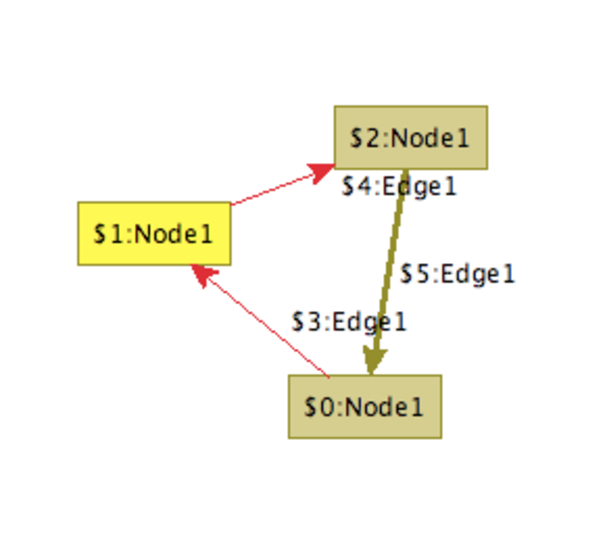
\includegraphics[width=0.25\linewidth]{fig/debug1}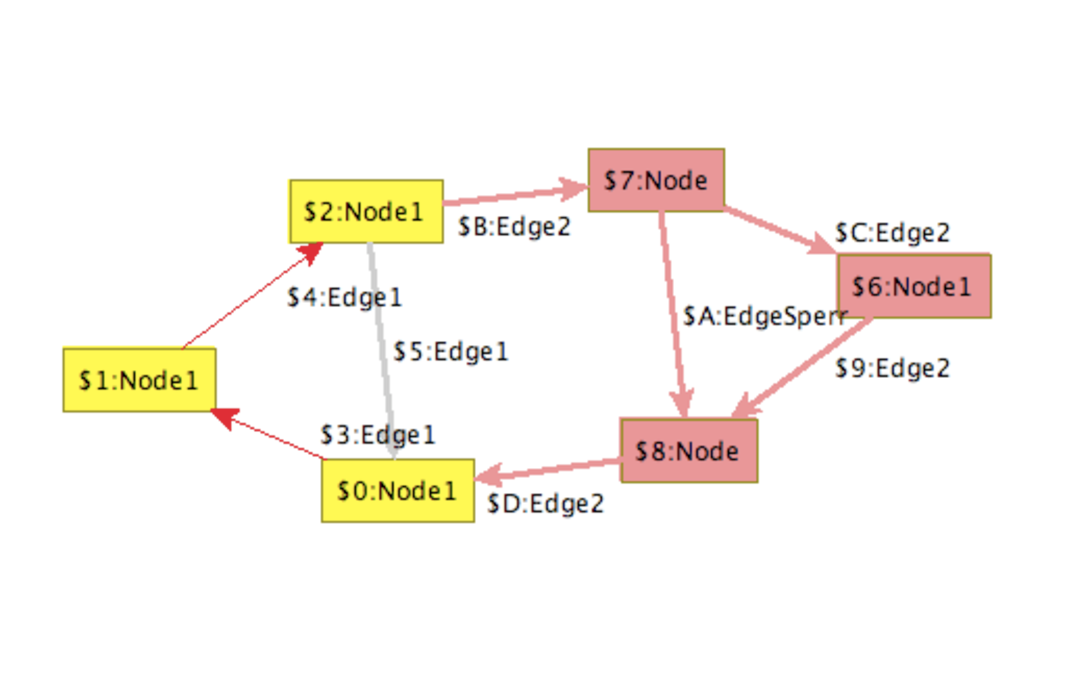
\includegraphics[width=0.4\linewidth]{fig/debug2}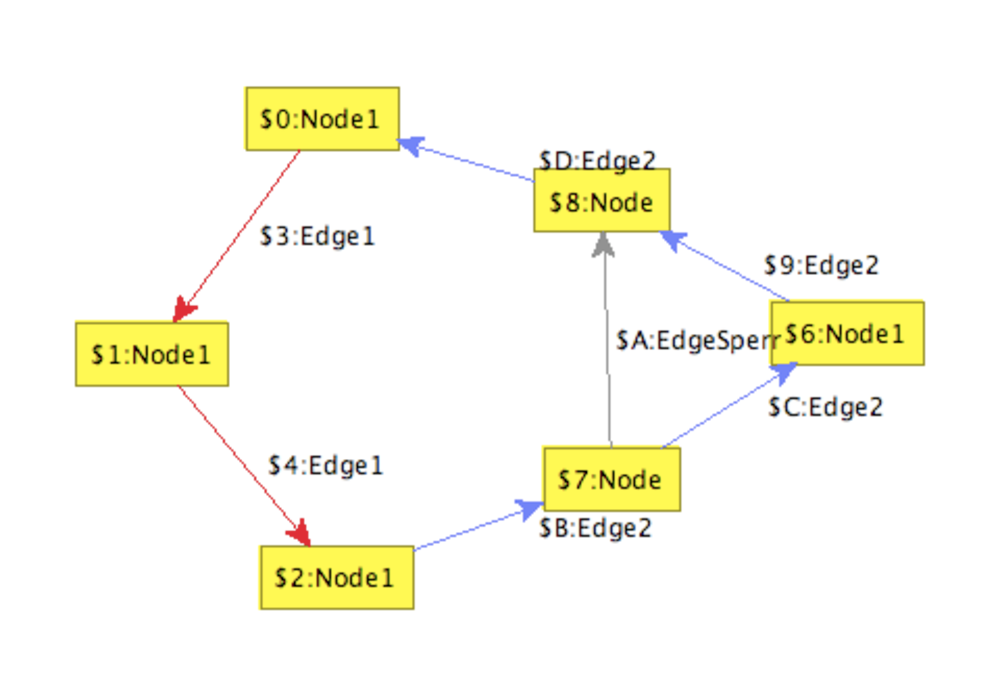
\includegraphics[width=0.4\linewidth]{fig/debug3}
%  \caption{Delayed step rule application.}
%  \label{figdebug}
%\end{figure}

\begin{figure}[htbp]
\begin{example}\label{ex:debug}  
We demonstrate the debug commands with a slightly adjusted script for the Koch snowflake from \GrG's examples (see also Section~\ref{fractals}). The graph rewriting sequence is
\begin{grshell}
debug xgrs (makeFlake1* & (beautify & doNothing)* & makeFlake2* & beautify*)[1]
\end{grshell}
\yComp\ will be opened with an initial graph (resulting from \texttt{grs init}):
\begin{center}
  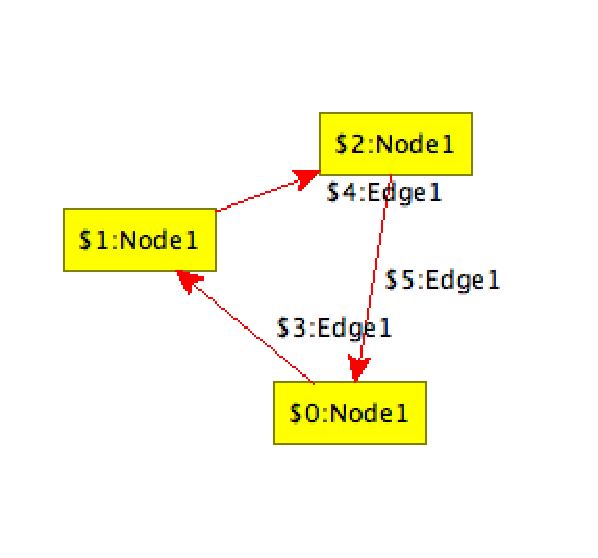
\includegraphics[width=0.3\linewidth]{fig/debug0tra}
\end{center}
We type \texttt{d}(etailed step) to apply \texttt{makeFlake1} step by step resulting in the following graphs:
\begin{center}
  \parbox{0.2\linewidth}{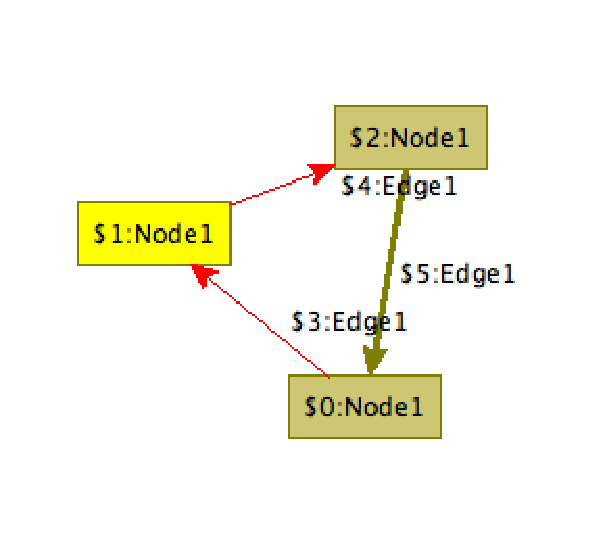
\includegraphics[width=\linewidth]{fig/debug1tra}}\parbox{0.375\linewidth}{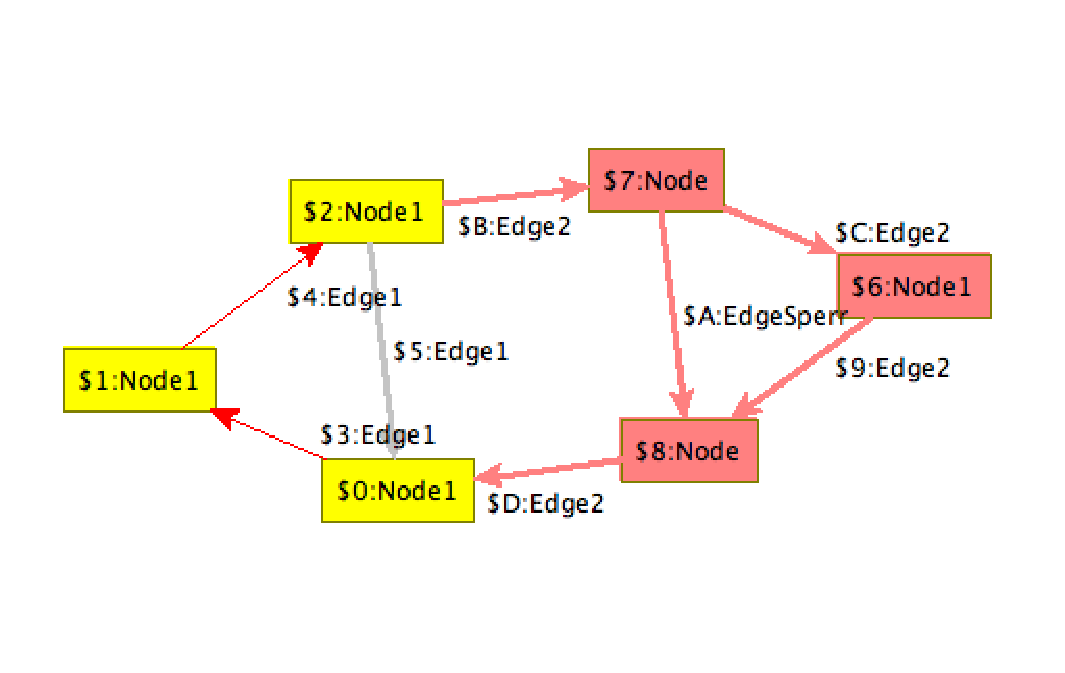
\includegraphics[width=\linewidth]{fig/debug2tra}}\parbox{0.375\linewidth}{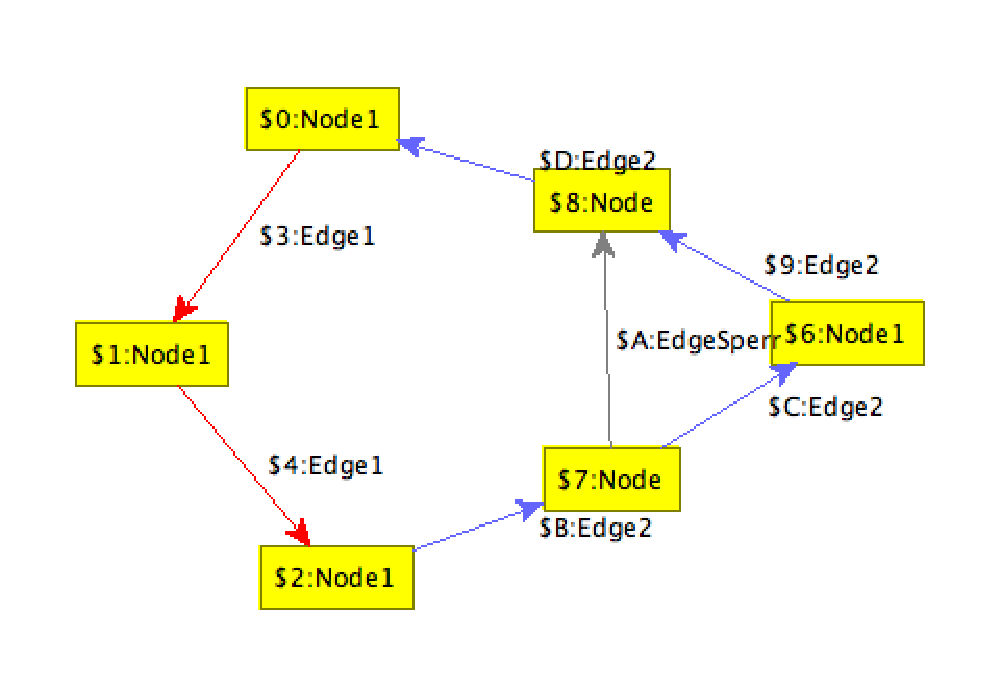
\includegraphics[width=\linewidth]{fig/debug3tra}}
\end{center}
The following table shows the ``break points'' of further debug commands, entered one after another:
\begin{center}
  \begin{tabular}{|l|l|} \hline
    \textbf{Command} & \textbf{Active rule} \\ \hline
    \texttt{s} & \texttt{makeFlake1} \\
    \texttt{o} & \texttt{beautify} \\
    \texttt{s} & \texttt{doNothing} \\
    \texttt{s} & \texttt{beautify} \\ 
    \texttt{u} & \texttt{beautify} \\ 
    \texttt{o} & \texttt{makeFlake2} \\
    \texttt{r} & --- \\ \hline
  \end{tabular}
\end{center}
\end{example}   
\end{figure}


\section{Backend Commands}
\label{backend}

\GrG\ is built to support multiple backends implementing the model and action interfaces of libGr.
This is roughly comparable to the different storage engines MySQL offers.
Currently only one backend is available, the libGr search plan backend, or short LGSPBackend.

\subsection{Backend selection and custom commands}

\begin{rail}
  'select' 'backend' Filename ( ( ) | ':' Parameters )
\end{rail}\ixkeyw{select}\ixkeyw{backend}
Selects a \indexed{backend} that handles graph and rule representation.
\emph{Filename} has to be a .NET assembly (e.g.\ \texttt{lgspBackend.dll}\indexmain{LGSPBackend}).
Comma-separated \indexed{parameter}s can be supplied optionally; if so, the backend must support these parameters.
By default the LGSPBackend is used.

\begin{rail}
  'show' 'backend'
\end{rail}\nopagebreak\ixkeyw{show}\ixkeyw{backend}
List all the parameters supported by the currently selected backend.
The parameters can be provided to the \texttt{select backend} command.

\begin{rail}
  'custom' 'graph' ( ( ) | SpacedParameters )
\end{rail}\ixkeyw{custom}\ixkeyw{graph}
Executes a command specific to the current backend.
If \emph{SpacedParameters} is omitted, a list of available commands will be displayed (for the LGSP backend see Sections~\ref{custom}).


\subsection{LGSPBackend Custom Commands}
\label{custom}

The \indexed{LGSPBackend} supports the following custom commands:

\begin{rail}
  'custom' 'graph' ('analyzegraph' | 'analyze') 
\end{rail}\ixkeyw{custom}\ixkeyw{graph}\ixkeyw{analyze}\ixkeyw{analyzegraph}
Analyzes\indexmain{analyzing graph} the current working graph.
The analysis data provides vital information for efficient \indexed{search plan}s.
Analysis data is available as long as \GrShell\ is running, i.e.\ when the working graph changes, the analysis data is still available but maybe obsolete.

\begin{rail}
  'custom' 'graph' 'setmaxmatches' Number
\end{rail}\ixkeyw{custom}\ixkeyw{graph}\ixkeyw{setmaxmatches}
Sets the maximum amount of possible pattern matches to \emph{Number}.
This command affects the expression \texttt{[\emph{Rule}]}.
If \emph{Number} is less or equal to zero, the constraint is reset.

\begin{rail}
  'custom' 'graph' 'optimizereuse' BoolLit
\end{rail}\ixkeyw{custom}\ixkeyw{graph}\ixkeyw{optimizereuse}
If set to false it prevents deleted elements from getting reused in a rewrite (i.e. it disables a performance optimization).
If set to true, new elements may not be discriminable anymore from already deleted elements using object equality, hash maps, etc.
					
\begin{rail}
  'custom' 'actions' 'gensearchplan' (Action+)
\end{rail}\ixkeyw{custom}\ixkeyw{actions}\ixkeyw{gensearchplan}
Creates a search plan (and executable code from it) for each rewrite rule \emph{Action} using the data from analyzing the graph (\texttt{custom graph analyze}).
Otherwise a \indexed{default search plan} is used. 
Analyzing and search plan/code generation themselves take some time, but they can lead to massively faster pattern matching, thus overall execution times
(the less uniform the type distribution and edge wiring between the nodes is, the higher are the improvements to be expected).
During the analysis phase the host graph must be in a shape ``similar'' to its shape when the main amount of work is done
(there may be some trial-and-error steps at different time points needed to get the overall most efficient search plan.)
A search plan is available as long as the current rule set remains loaded. 
Specify multiple rewrite rules instead of using multiple commands for each rule to improve the search plan generation performance.

\begin{rail}
  'custom' 'actions' 'dumpsourcecode' BoolLit
\end{rail}\ixkeyw{custom}\ixkeyw{actions}\ixkeyw{dumpsourcecode}
If set to true, C\# files will be dumped for the newly generated searchplans (similar to the \texttt{-keep} option of the generator).



\chapter{Visualization and Debugging}\indexmain{Debugger}
\label{chapdebugger}

This chapter gives an introduction into the visualization capabilites of yComp and into the graphical debugger of \GrG, which is offered by \GrShell\ in combination with yComp.

Other commands of use for debugging were already introduced in the shell chapter:
\verb#show var <Variable># to print the content of a variable (but pressing the \texttt{v} key in the shell debugger is a lot more convenient) and \verb#show <GraphElement>.<AttributeName># to print the content of an attribute (but searching with \texttt{Ctrl-f} or \texttt{/} in yComp for the persistent name or an attribute value, hovering over the then highlighted graph element is more convenient, again); furthermore \verb#record# and \verb#replay# are interesting when you are debugging a transformation where you are choosing from the available matches by hand and want to try other paths later by choosing differently on a previous match: they allow you to save and restore graph states of interest, and to inspect the sequence of changes which lead to them in the \texttt{.grs}.

%%%%%%%%%%%%%%%%%%%%%%%%%%%%%%%%%%%%%%%%%%%%%%%%%%%%%%%%%%%%%%%%%%%%%%%%%%%%%%%%%%%%%%%%%%%%%%%%
\section{Graph Visualization Commands (Nested Layout)}\label{sub:visual}\indexmain{visualization}\indexmainsee{layout}{visualization}\indexmainsee{visualization}{group node}\indexmain{nested layout}\indexmainsee{nested layout}{group node}\indexmain{nested graph}\indexmainsee{nested graph}{group node}

\begin{rail}
  'show' 'graph' ExecutableName (() | Text)
\end{rail}\ixkeyw{show}\ixkeyw{graph}
Dumps the current graph in \indexed{VCG} format into a temporary file.
The temporary VCG file will be passed to the program \emph{ExecutableName} as first parameter;
further parameters, such as program options, can be specified by \emph{Text}.
If you use \yComp\footnote{See Section~\ref{tools:ycomp}.}\indexmain{yComp} as executable (\texttt{show graph ycomp}), this may look like
\begin{center}
  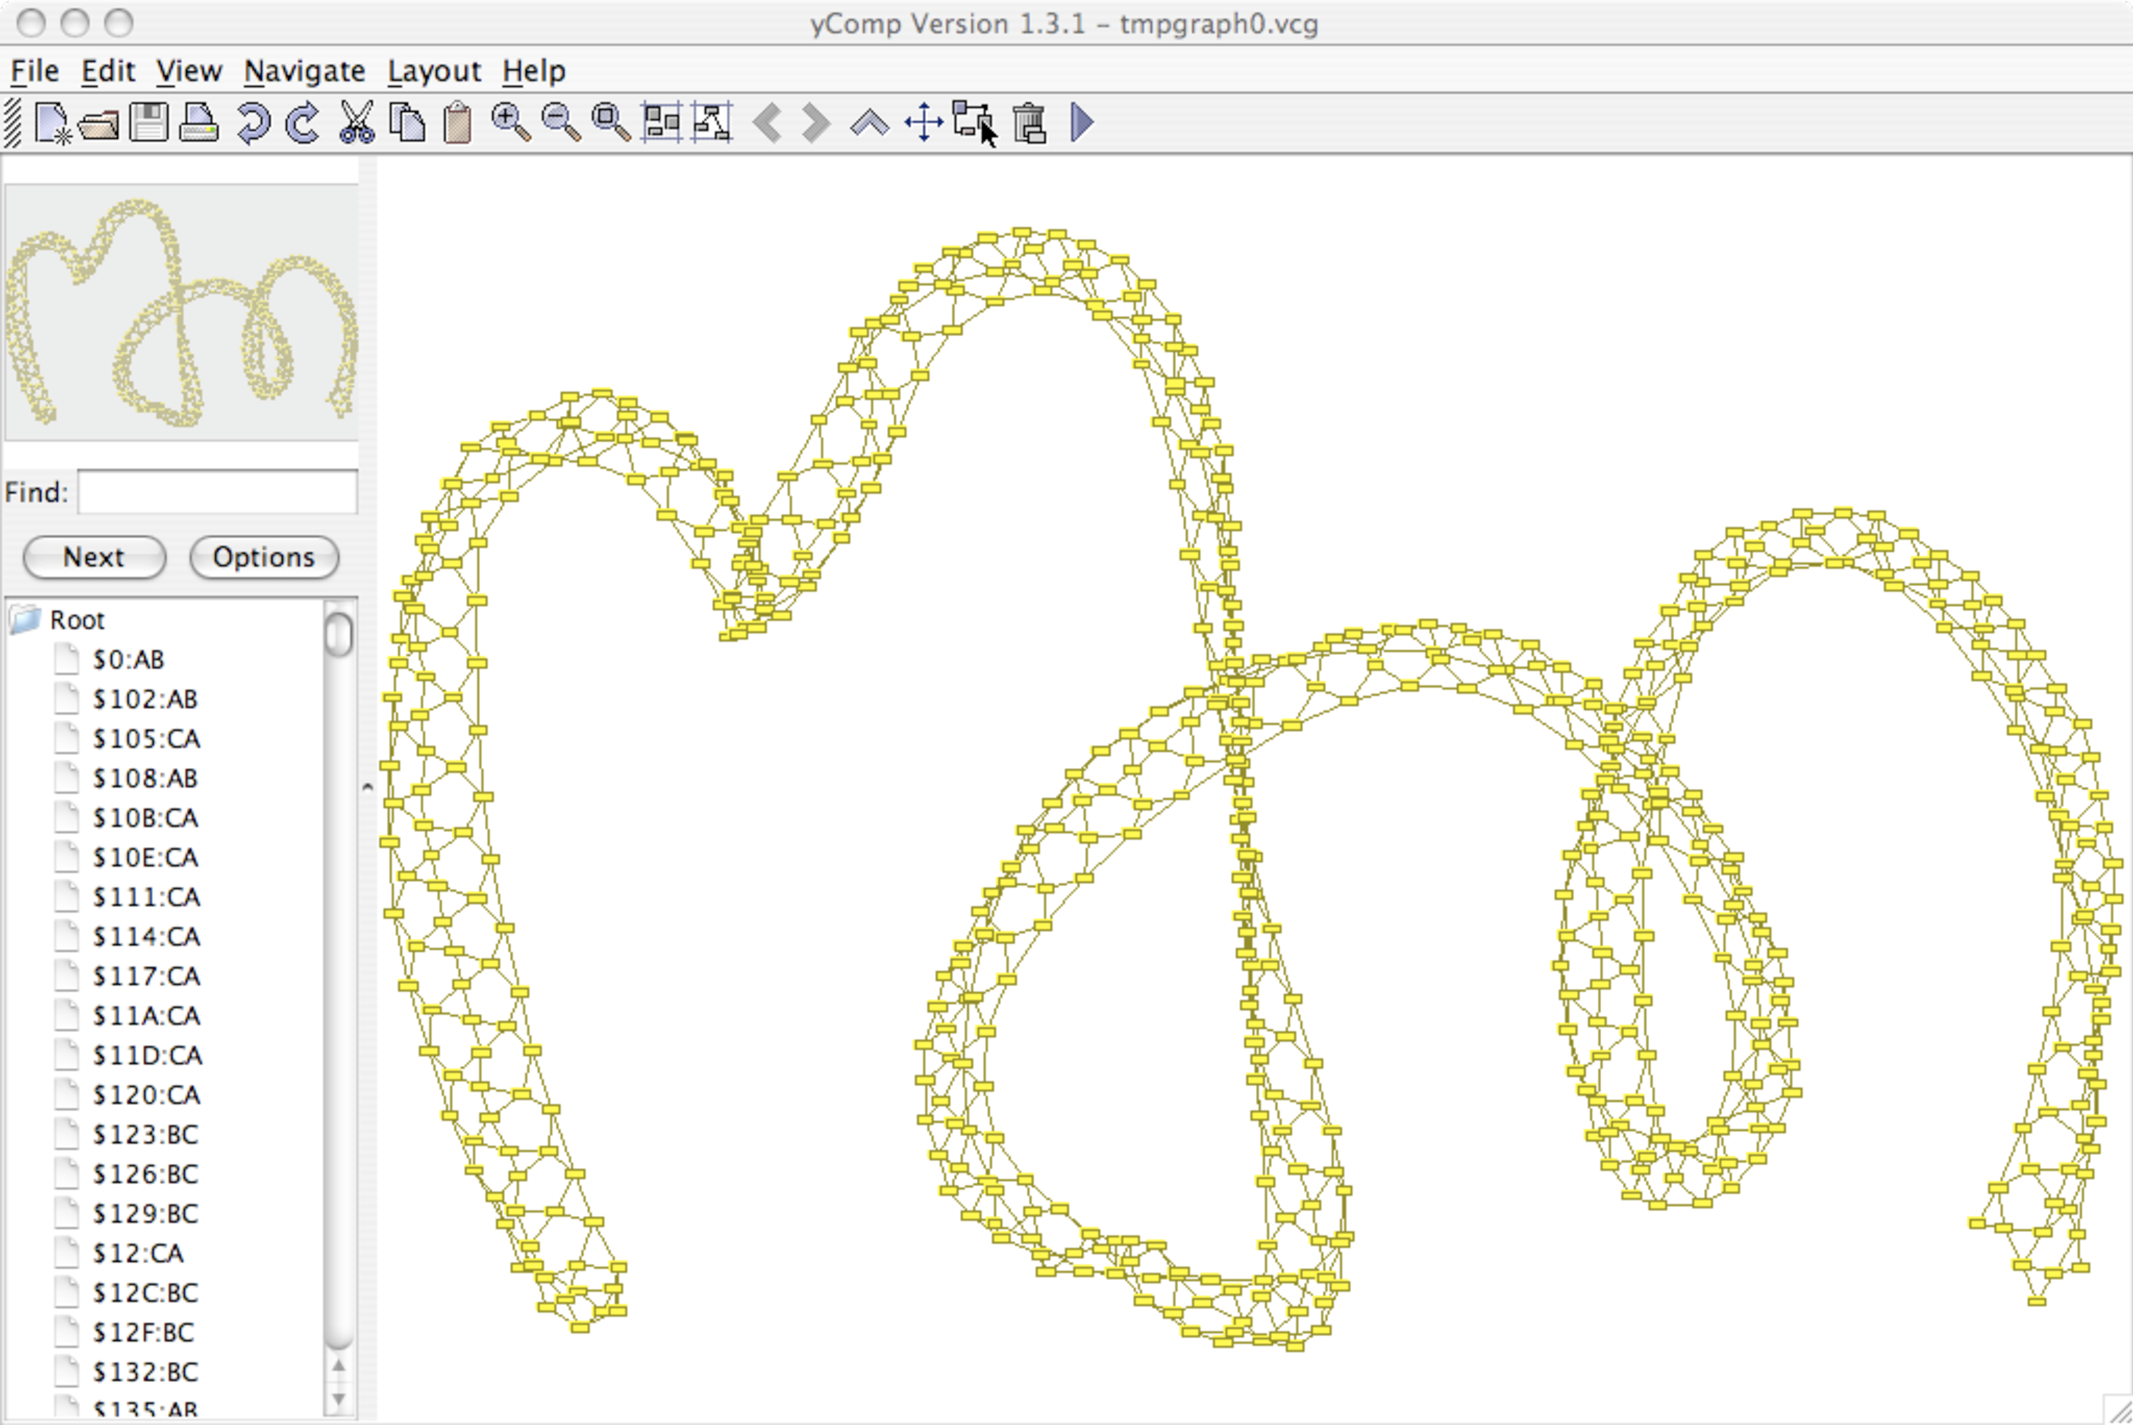
\includegraphics[width=0.75\linewidth]{fig/showgraph}
\end{center}  
The temporary file will be deleted, when the application \emph{Filename} is terminated if \GrShell\ is still running at this time.

\begin{rail}
  'dump' 'graph' Filename
\end{rail}\ixkeyw{dump}\ixkeyw{graph}
Dumps the current graph in \indexed{VCG} format into the file \emph{Filename}.\\

The following commands control the style of the VCG output. This affects \texttt{dump graph}, \texttt{show graph}, and \texttt{enable debug}. 
\begin{rail}
  'dump' 'set' 'node' (() | 'only') NodeType \\ (('color' | 'textcolor' | 'bordercolor') Color | 'shape' Text | 'labels' ('on' | 'off' | Text)) ;
\end{rail}\ixkeyw{dump}\ixkeyw{set}\ixkeyw{node}\ixkeyw{only}\ixkeyw{color}\ixkeyw{textcolor}\ixkeyw{bordercolor}\ixkeyw{shape}\ixkeyw{labels}\ixkeyw{on}\ixkeyw{off}
Sets the \indexed{color}, text color, border color, the shape or the label of the nodes of type \emph{NodeType} and all of its subtypes.
The keyword \texttt{only} excludes the subtypes. The available colors are specified at the begin of this chapter. 
The following shapes are supported: \texttt{box}, \texttt{triangle}, \texttt{circle}, \texttt{ellipse}, \texttt{rhomb}, \texttt{hexagon}, \texttt{trapeze}, \texttt{uptrapeze}, \texttt{lparallelogram}, \texttt{rparallelogram}.
Those are shape names of \yComp\ (for a VCG definition see~\cite{vcg}).
The following colors are supported: \texttt{Black}, \texttt{Blue}, \texttt{Green}, \texttt{Cyan}, \texttt{Red}, \texttt{Purple}, \texttt{Brown}, \texttt{Grey}, \texttt{LightGrey}, \texttt{LightBlue}, \texttt{LightGreen}, \texttt{LightCyan}, \texttt{LightRed}, \texttt{LightPurple}, \texttt{Yel\-low}, \texttt{White}, \texttt{DarkBlue}, \texttt{DarkRed}, \texttt{Dark\-Green}, \texttt{DarkYellow}, \texttt{DarkMagenta}, \texttt{DarkCyan}, \texttt{Gold}, \texttt{Lilac}, \texttt{Turquoise}, \texttt{Aquamarine}, \texttt{Khaki}, \texttt{Pink}, \texttt{Orange}, \texttt{Orchid}.
These are the same color identifiers as in \indexed{VCG}/\yComp\ files (for a VCG definition see~\cite{vcg}).

The default labeling is set to \texttt{on} with \texttt{Name:Type}, it can be overwritten by an specified label string (e.g. the source code line originating the node in a program graph) or switched off.

\begin{rail}
  'dump' 'set' 'edge' (() | 'only') EdgeType \\ (('color' | 'textcolor') Color | 'labels' ('on' | 'off' | Text));
\end{rail}\ixkeyw{dump}\ixkeyw{set}\ixkeyw{edge}\ixkeyw{only}\ixkeyw{color}\ixkeyw{textcolor}\ixkeyw{labels}\ixkeyw{on}\ixkeyw{off}
Sets the color, text color or label of the edges of type \emph{EdgeType} and all of its subtypes.
The keyword \texttt{only} excludes the subtypes. The available colors are specified at the begin of this chapter.
The default labeling is set to \texttt{on} with \texttt{Name:Type}, it can be overwritten by an specified label string or switched off.

\begin{rail}
  'dump' 'add' (('node' ('only')? NodeType)|('edge' ('only')? EdgeType)) 'exclude' ;
\end{rail}\ixkeyw{dump}\ixkeyw{add}\ixkeyw{node}\ixkeyw{edge}\ixkeyw{only}\ixkeyw{exclude}
Excludes nodes/edges of type \emph{NodeType}/\emph{EdgeType} and all of its subtypes from output, for a node it also excludes its incident edges.
The keyword \texttt{only} excludes the subtypes from exlusion, i.e.\ subtypes of \emph{NodeType}/\emph{EdgeType} are dumped.

\begin{rail}
  'dump' 'add' 'node' ('only')? NodeType 'group' (GroupConstraints)? ;
GroupConstraints:
  'by' ('hidden')? GroupMode (IncAdjTypeConstraints)? ;
IncAdjTypeConstraints:
  ('only')? EdgeType ('with' ('only')? NodeType)? ;
\end{rail}\ixkeyw{dump}\ixkeyw{add}\ixkeyw{node}\ixkeyw{only}\ixkeyw{group}\ixkeyw{by}\ixkeyw{hidden}\ixkeyw{with}\ixnterm{GroupConstraints}\ixnterm{IncAdjTypeConstraints}
Declares \emph{NodeType} and subtypes of \emph{NodeType} as \indexed{group node}\indexmainsee{hierarchic}{group node} type.
All the differently typed nodes that point to a node of type \emph{NodeType} 
(i.e.\ there is a directed edge between such nodes) will be grouped and visibly enclosed by the \emph{NodeType}-node (nested graph).
\texttt{GroupMode} is one of \texttt{no},\texttt{incoming},\texttt{outgoing},\texttt{any}; \texttt{hidden} causes hiding of the edges by which grouping happens.
The \texttt{EdgeType} constrains the type of the edges which cause grouping, the \texttt{with} clause additionally constrains the type of the adjacent node; 
\texttt{only} excludes subtypes.

\begin{note}
Only apply group commands on a graph if they indeed lead to a containment tree of groups.
If the group commands would lead to a directed acyclic or even cyclic containment graph, the results are undefined.
You may get duplicate edges (and nodes); the implementation is free to choose indeterministically between the possible nestings -- it may even grow an arm and stab you in your back.
(A conflict resultion heuristic used is to give the earlier executed \texttt{add group} command priority. 
But this mechanism is incomplete -- you'd better refine your groups or change the model in that case.
Using a model separating edges denoting direct containment from cross-linking edges by type is normally the better design, even disregarding visual node nesting.)
\end{note}

The following example shows \emph{metropolis} ungrouped and grouped:
\begin{center}
  \fbox{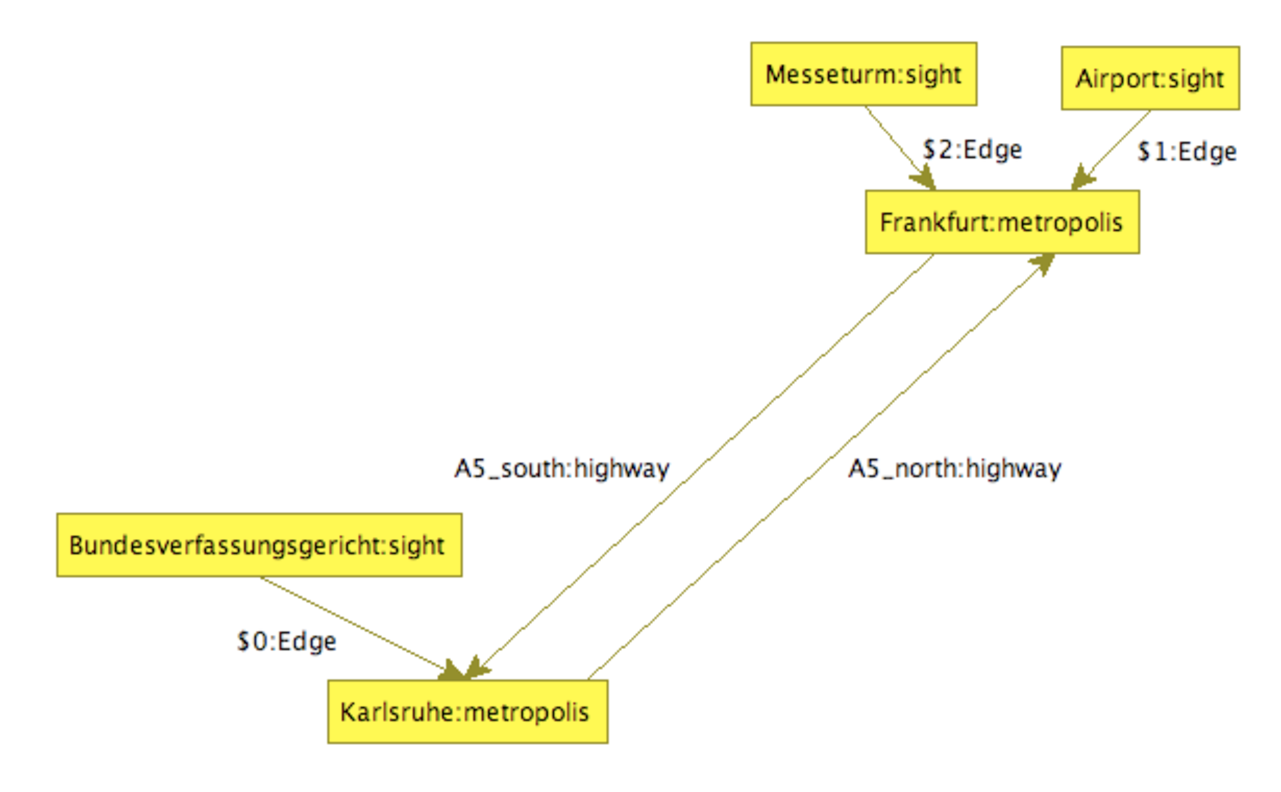
\includegraphics[width=0.45\linewidth]{fig/group2-1}}  \hfill \fbox{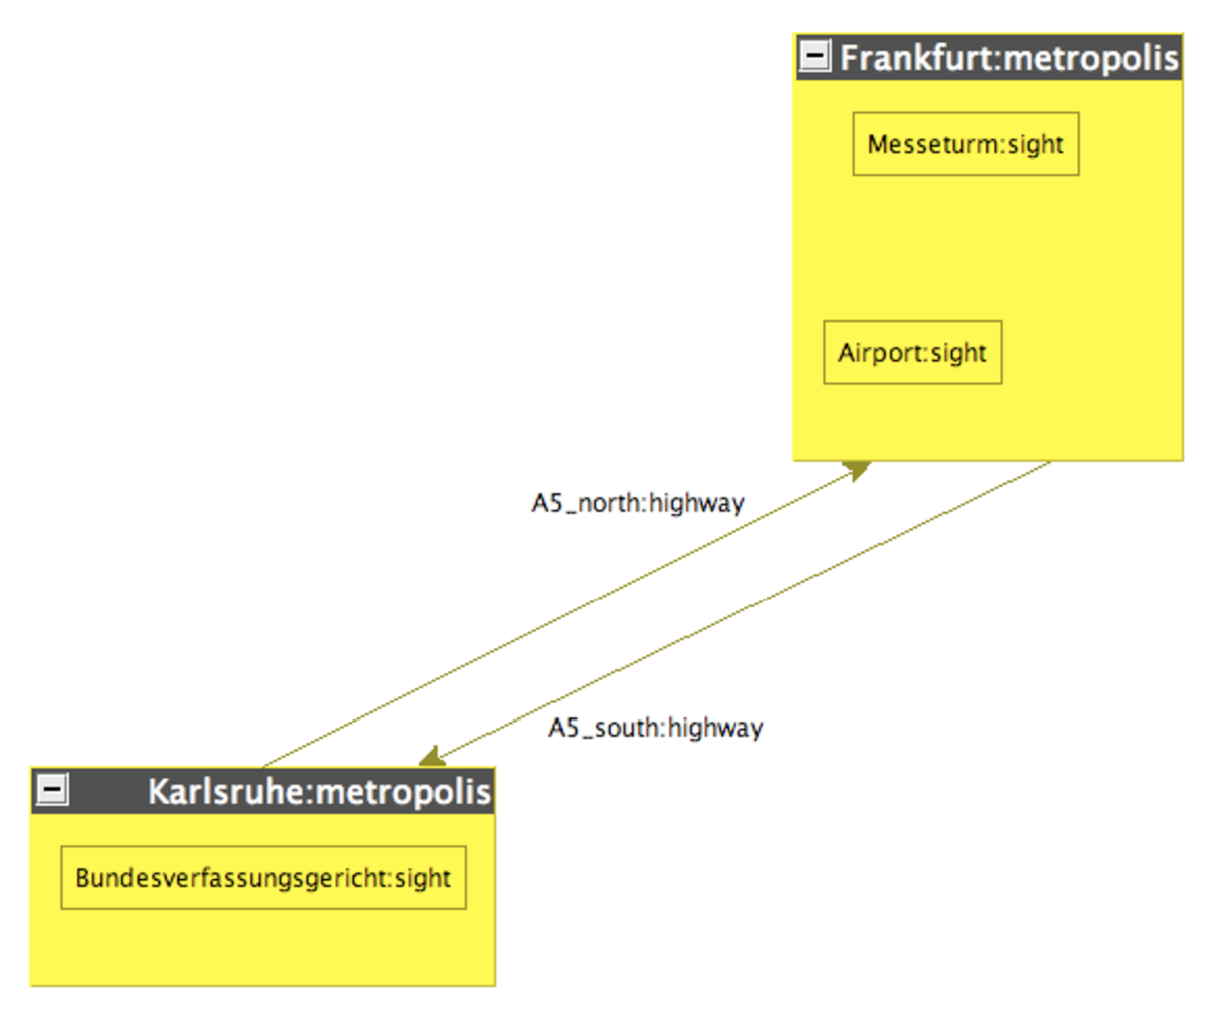
\includegraphics[width=0.45\linewidth]{fig/group2-2}}\\
  {\small right side: dumped with \texttt{dump add node metropolis group}}
\end{center}

\begin{rail}
  'dump' 'add' (() | 'only') ('node' NodeType | 'edge' EdgeType) \\ ('infotag' | 'shortinfotag') AttributeName
\end{rail}\ixkeyw{dump}\ixkeyw{add}\ixkeyw{only}\ixkeyw{node}\ixkeyw{edge}\ixkeyw{infotag}\ixkeyw{shortinfotag}
Declares the \indexed{attribute} \emph{AttributeName} to be an ``\indexed{info tag}'' or ``\indexed{short info tag}''.
Info tags are displayed like additional node/edge \indexed{label}s, in format \texttt{Name=Value}, or \texttt{Value} only for short info tags. 
The keyword \texttt{only} excludes the subtypes of \emph{NodeType} resp.\ \emph{EdgeType}. 
In the following example \emph{river} and \emph{jam} are info tags:
\begin{center}
  \fbox{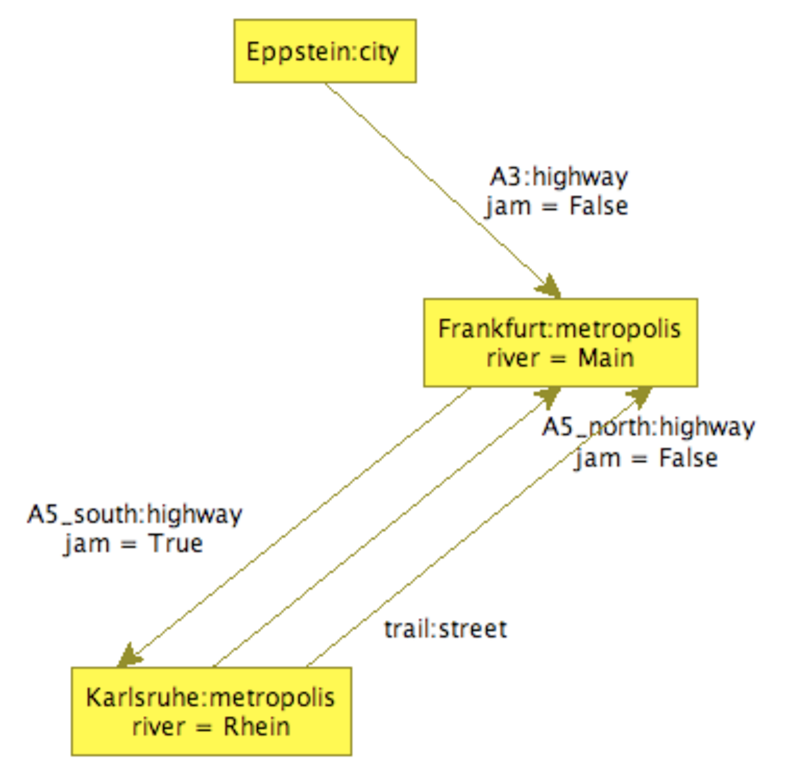
\includegraphics[width=0.5\linewidth]{fig/infotag}}
\end{center}

\begin{rail}
  'dump' 'reset'
\end{rail}\ixkeyw{dump}\ixkeyw{reset}
Resets all style options (\texttt{dump set}\dots) and (\texttt{dump add}\dots) to their default values.


\begin{note}\label{note:visual}
Small graphs allow for fast visual understanding, but with an increasing number of nodes and edges they quickly loose this property.
The group commands are of outstanding importance to keep readability with increasing graph sizes
(e.g. for program graphs it allows to lump together expressions of a method inside the method node and attributes of the class inside the class node).
Additional helpers in keeping the graph readable are: 
the capability to exclude elements from dumping (the less hay in the stack the easier to find the needle),
the different colors and shapes to quickly find the elements of interest,
as well as the labels/infotags/shortinfotags to display the most important information directly. 
Choose the layout algorithm and the options delivering the best results for your needs, organic and hierarchic or compiler graph 
(an extension of hierarchic with automatic edge cutting -- marking cut edges by fat dots, showing the edge only on mouse over and allowing to jump to the other end on a mouse click)
should be tried first.
\end{note}

The following example shows several of the layout options employed to considerably increase the readability of a program graph (as given in \texttt{examples/JavaProgramGraphs-GraBaTs08}):
\begin{figure}[htbp]
  \centering
  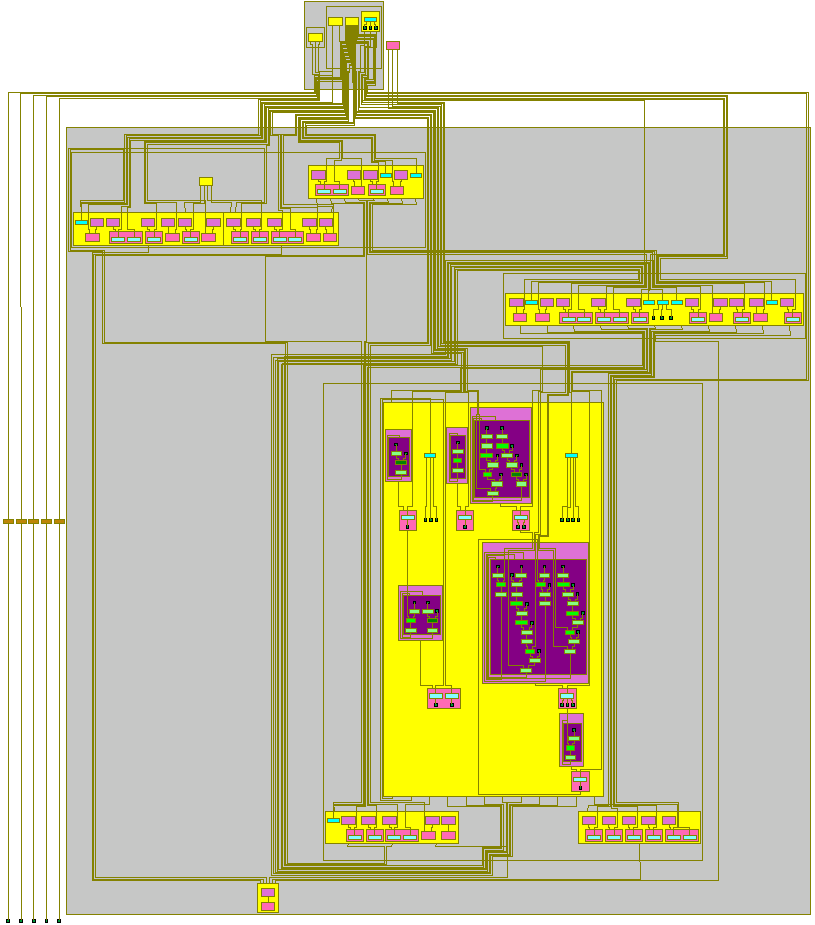
\includegraphics[width=0.8\textwidth]{fig/screen-overview}
  \caption{Overview of the initial program graph }
  \label{figprogramgraph1}
\end{figure}

\begin{figure}[htbp]
  \centering
  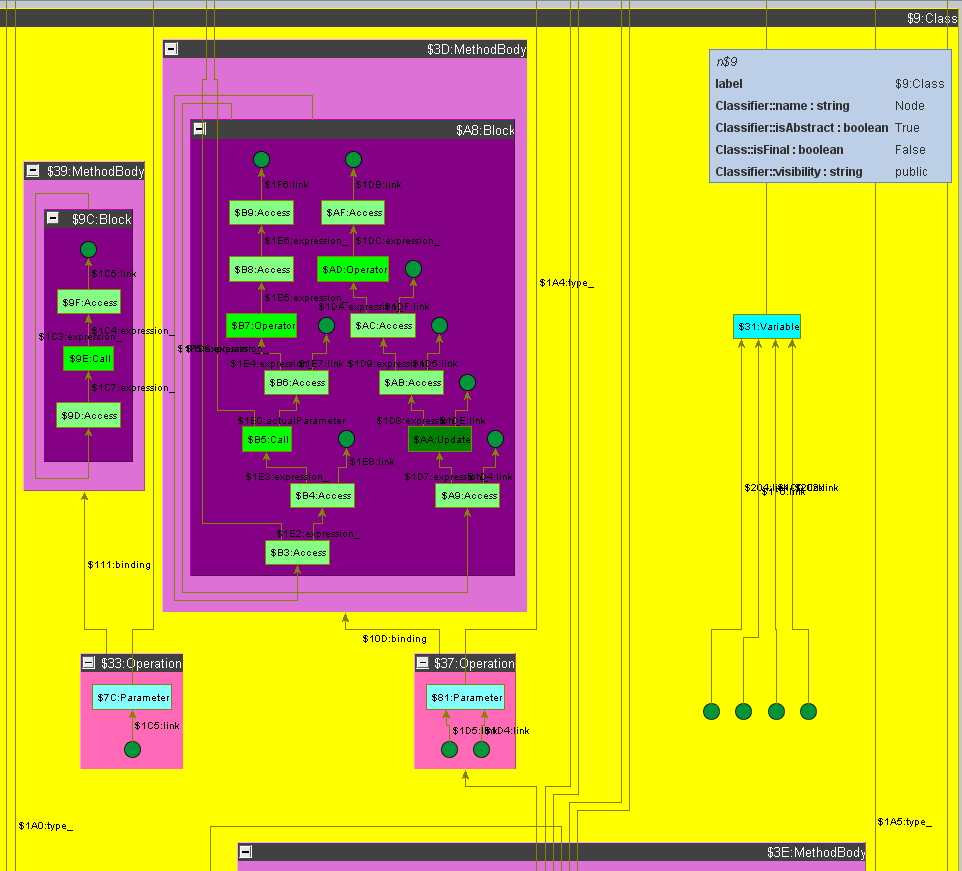
\includegraphics[width=0.7\textwidth]{fig/screen-detail}
  \caption{Some details of the ``Node'' class of the initial program graph}
  \label{figprogramgraph2}
\end{figure}


%%%%%%%%%%%%%%%%%%%%%%%%%%%%%%%%%%%%%%%%%%%%%%%%%%%%%%%%%%%%%%%%%%%%%%%%%%%%%%%%%%%%%%%%%%%%%%%%
\section{Debugging Related Commands}

\begin{rail}
  'debug' ( 'enable' | 'disable' )
\end{rail}\ixkeyw{debug}\ixkeyw{enable}\ixkeyw{disable}
Enables and disables the \indexed{debug mode}.
The debug mode shows the current working graph in a \yComp\ window.
All changes to the working graph are tracked by \yComp\ immediately.  

\begin{rail}
  'debug' 'set' 'layout' ( (Text)? | 'option' Name String ) ;
\end{rail}\ixkeyw{debug}\ixkeyw{set}\ixkeyw{layout}\ixkeyw{option}
Sets the default graph \indexed{layout algorithm} to \emph{Text}.
If \emph{Text} is omitted, a list of the available layout algorithms is displayed.
The following layout algorithms are supported: \texttt{Random}, \texttt{Hierarchic}, \texttt{Organic}, \texttt{Orthogonal}, \texttt{Circular}, \texttt{Tree}, \texttt{Diagonal}, \texttt{Incremental Hierarchic}, \texttt{Compilergraph}.
For technical graphs \texttt{Hierarchic} works normally best; \texttt{Compilergraph} is a version of \texttt{Hierarchic} cutting some edges, it may be of interest if \texttt{Hierarchic} contains too many crossing edges. \texttt{Organic} is the other general purpose layout available, the other layouts are rather special, but this should not prevent you from using them if they fit to your task ;).
The \texttt{option} version allows to specify layout options by name value pairs.
The available layout options can be listed by the following command.
 
\begin{rail}
  'debug' 'get' 'layout' 'options';
\end{rail}\ixkeyw{debug}\ixkeyw{get}\ixkeyw{layout}\ixkeyw{options}
Prints a list of the available layout options of the layout algorithm.

\begin{rail}
  'debug' 'layout';
\end{rail}\ixkeyw{debug}\ixkeyw{layout}
Forces re-layout of the graph shown in yComp (same as pressing the play button within yComp).

\begin{rail}
  GraphRewriteSequence: 'debug' 'xgrs' SimpleRewriteSequence ;
\end{rail}\ixkeyw{debug}\ixkeyw{xgrs}\indexmain{graph rewrite sequence}\indexmainsee{GRS}{graph rewrite sequence}\ixnterm{GraphRewriteSequence}
This executes the graph rewrite sequence \emph{SimpleRewriteSequence} in the debugger\indexmain{debugger}.
Same as \texttt{xgrs SimpleRewriteSequence} in the previous chapter, but allows tracing the rewriting process step-by-step. 


%%%%%%%%%%%%%%%%%%%%%%%%%%%%%%%%%%%%%%%%%%%%%%%%%%%%%%%%%%%%%%%%%%%%%%%%%%%%%%%%%%%%%%%%%%%%%%%%
\section{Using the Debugger}

The debugging process follows of a series of debug situations,
which result from a user selection of the underlying execution situations accoring to interest.
During each debugging step the debugger\indexmain{debugger} -- which is a part of the \GrShell~-- 
prints the debugged sequence with the currently focused/active rule highlighted yellow.
What will be shown from executing this rule depends on the commands chosen by the user;
and on the fact whether the focused rule matches or not.
An active rule which is already known to match is highlighted green.
The rules which matched during sequence execution are shown on dark green background,
the rules which failed during sequence execution are shown on dark red background;
at the begin of a new loop iteration the highlighting state of the contained rules is reset.
During execution \yComp\footnote{Make sure, that the path to your \texttt{\indexed{yComp.jar}} package is set correctly in the \texttt{ycomp} shell script within \GrG's \texttt{/bin} directory.}\indexmain{yComp}
will display the changes to the graph from every single step. 
Besides deciding on what is shown from the execution of the current rule, 
the user determines with the debug commands where to continue the execution
(the rule focused next; but again this depends on success/failure of the currently active rule).
The debug commands are given in Table~\ref{tabdebug}.
A run is shown in the following example \ref{ex:debug}.

In addition to the commands for actively stepping or skipping through the sequence exection,
there are breakpoints and choicepoints available (toggled with the \texttt{b} and \texttt{c} commands)
which are only processed when they are reached, but on the other hand are also processed if a user command would skip them.
The \indexed{break point}s halt execution, focus the reached sequence, and cause the debugger to wait for further commands
(e.g. \texttt{d} to inspect the rule execution en detail versus \texttt{s} for just applying it).
The \indexed{choice point}s halt execution, focus the reached sequence in magenta, and ask for some user input; 
after the input was received, execution continues according to the command previously issued.
Both break points and choice points are denoted by the \texttt{\%} modifier. 
The \texttt{\%} modifier works as a break point if it is given before: a rule, an all bracketed rule, a variable predicate, or the constants \texttt{true}/\texttt{false}.
The \texttt{\%} modifier works as a choice point if it is appended to the \texttt{\$} randomize modifier switching a random decision into a user decision.
This holds for the binary operators, the random match selector of all bracketed rules, the random-all-of operators and the one-of-set braces.
The idea behind this is: you need some randomization for \indexed{simulation} purposes --- then use the randomize modifier \texttt{\$}.
You want to force a certain decision overriding the random decision to try out another execution path while debugging the simulation flow --- then modify the randomize modifier with the user (choice) modifier \texttt{\%}.

The initial breakpoint and choicepoint assignment is given with the \texttt{\%} characters in the sequences after the \texttt{debug xgrs} commands in the \texttt{.grs} file.
The breakpoint and choicepoint commands of the debugger allow to toggle them at runtime, overriding the initial assignment (notationally yielding a sequence with added or removed \texttt{\%} characters).
The user input commands \texttt{\$\%(type)} define choice points which can't be toggled off.

Further commands allow to print the variables at a given situation, the sequence call stack, or a full state dump of the call stack and the variables.

\begin{table}[htbp]
  \begin{tabularx}{\linewidth}{|lX|}
\hline
  \texttt{s}(tep) & Execute the current rewrite rule (match, and rewrite in case it matched; the resulting graph is shown).\\
  \texttt{d}(etailed step) & Execute the current rewrite rule in a three-step procedure: matching - highlighting the found match, rewriting - highlighting the changing elements, and doing the rewrite showing the resulting graph. In addtion, afterwards the execution of subrules from embedded xgrs (\texttt{exec}) is shown step by step. \\
  (step) \texttt{o}(ut) & Continue execution until the end of the current loop. If the execution is not in a loop at this moment, but in a sequence called, the called sequence will be executed until its end. If neither is the case, the complete sequence will be executed.\\
  (step) \texttt{u}(p) & Ascend one level up within the \indexed{Kantorowitsch tree} of the current rewrite sequence (i.e. rule; see Example~\ref{ex:debug}; at the moment the command is pretty useless because only the serialized form is displayed).\\
  \texttt{r}(un) & Continue execution (until the end or a breakpoint).\\
  \texttt{a}(bort) & Cancel the execution immediately.\\
  \texttt{n}(ext) & Go to the next rewrite rule which matches, make it current.\\
\hline
  (toggle) \texttt{b}(reakpoint) & Toggle a breakpoint at one of the breakpointable locations.\\
  (toggle) \texttt{c}(choicepoint) & Toggle a choicepoint at one of the choicepointable locations.\\
\hline
  \texttt{v}(ariables) & Prints the global variables and the local variables of the sequence currently executed, which is the topmost sequence of the sequence call stack. To be more precise regarding local variables: all variables which were defined (and have not fallen out of scope again) up to the sequence position focussed.\\
  \texttt{t}(race) & Prints the stack trace of the current sequence call stack; the stack trace includes the body of each sequence called at its execution state.\\
  \texttt{f}(ull dump) & Prints the stack trace including the local variables of each stack frame plus the global variables.\\
\hline 
  \end{tabularx}
  \caption{\GrShell\ debug commands}
  \label{tabdebug}
\end{table}
%\begin{figure}[htbp]
%  \centering
%  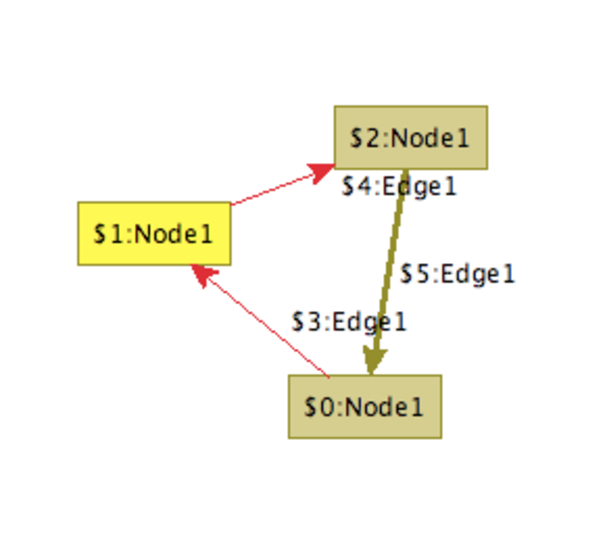
\includegraphics[width=0.25\linewidth]{fig/debug1}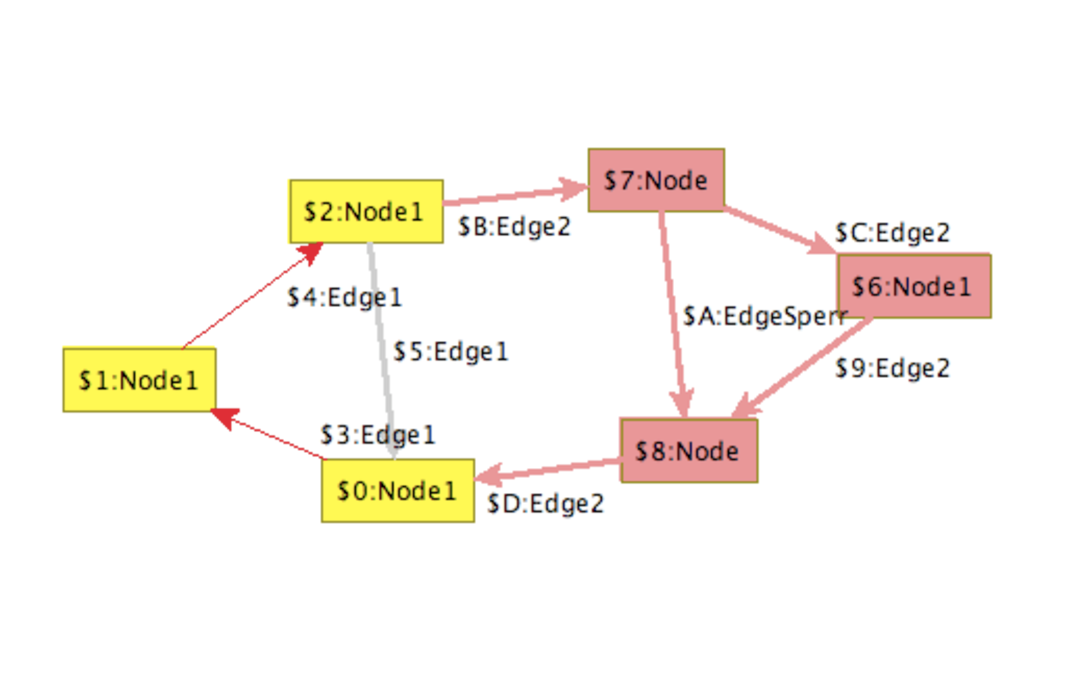
\includegraphics[width=0.4\linewidth]{fig/debug2}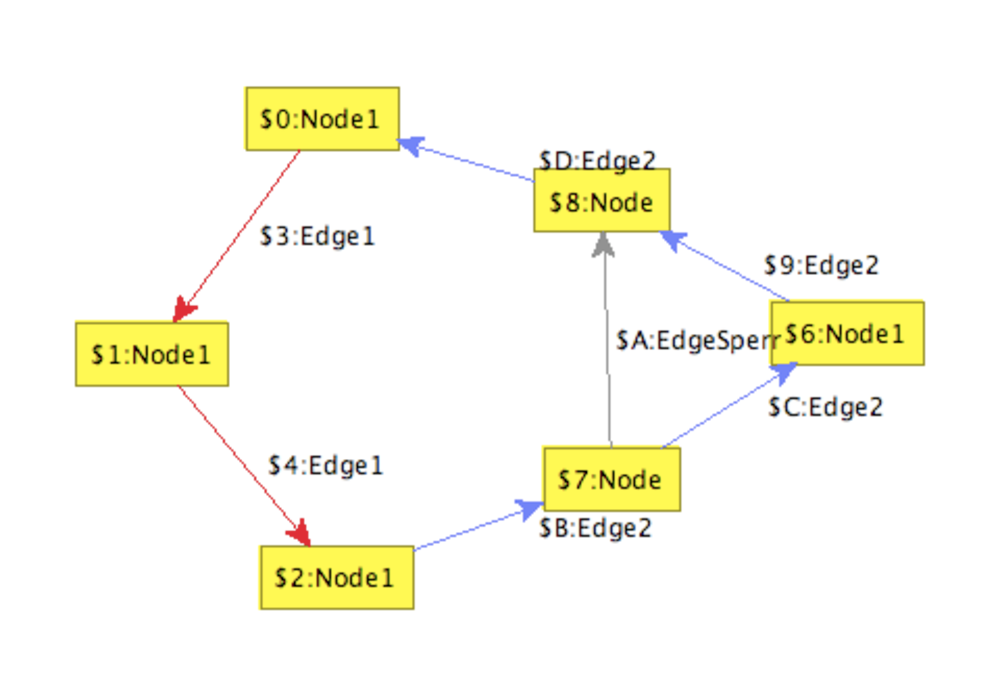
\includegraphics[width=0.4\linewidth]{fig/debug3}
%  \caption{Delayed step rule application.}
%  \label{figdebug}
%\end{figure}

\pagebreak

\begin{figure}[htbp]
\begin{example}\label{ex:debug}  
We demonstrate the debug commands with a slightly adjusted script for the Koch snowflake from \GrG's examples (see also Section~\ref{fractals}). The graph rewriting sequence is
\begin{grshell}
debug xgrs (makeFlake1* & (beautify & doNothing)* & makeFlake2* & beautify*)[1]
\end{grshell}
\yComp\ will be opened with an initial graph (resulting from \texttt{grs init}):
\begin{center}
  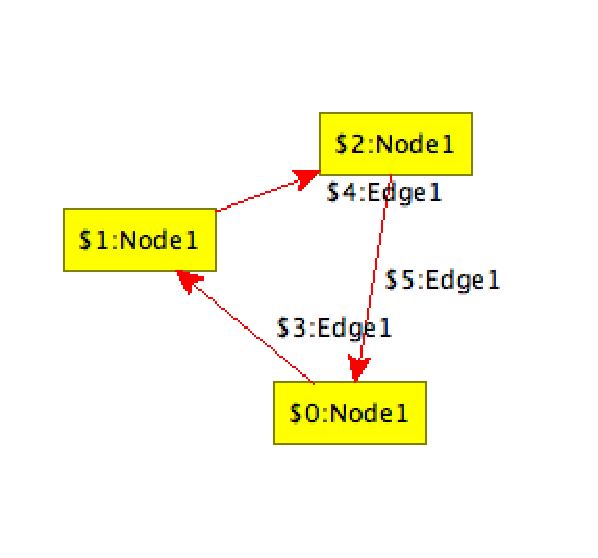
\includegraphics[width=0.3\linewidth]{fig/debug0tra}
\end{center}
We type \texttt{d}(etailed step) to apply \texttt{makeFlake1} step by step resulting in the following graphs:
\begin{center}
  \parbox{0.2\linewidth}{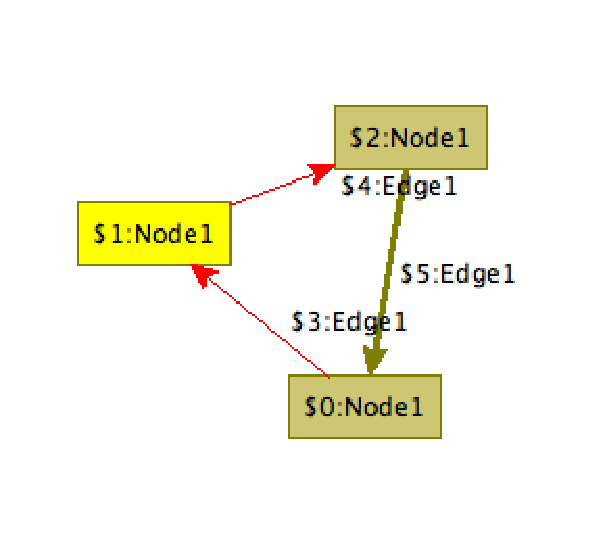
\includegraphics[width=\linewidth]{fig/debug1tra}}\parbox{0.375\linewidth}{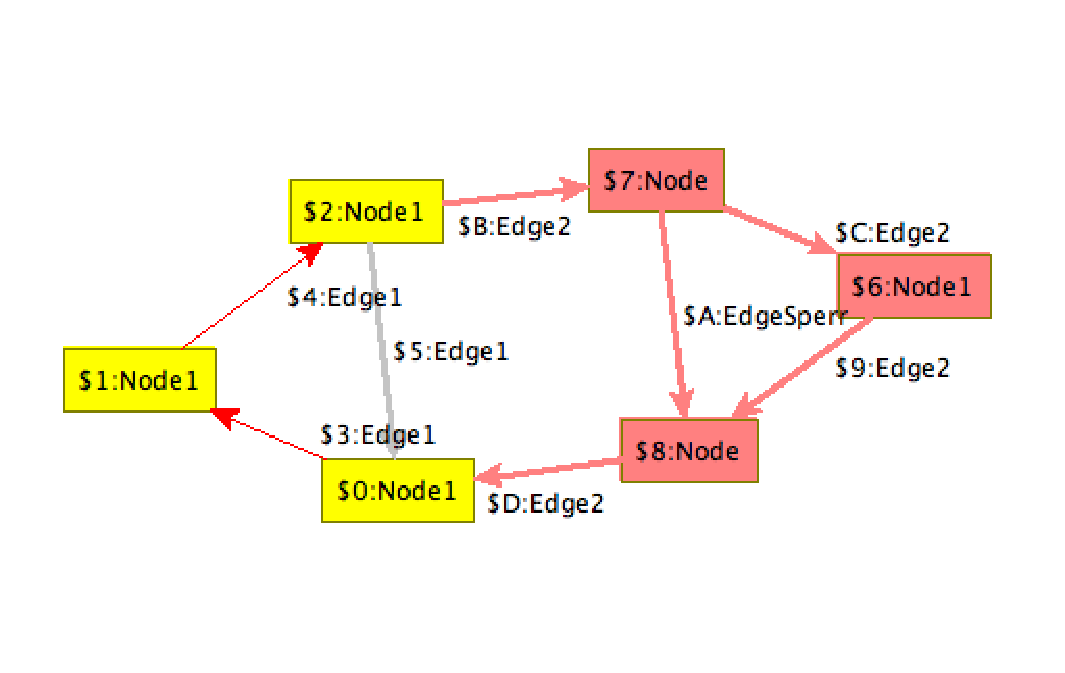
\includegraphics[width=\linewidth]{fig/debug2tra}}\parbox{0.375\linewidth}{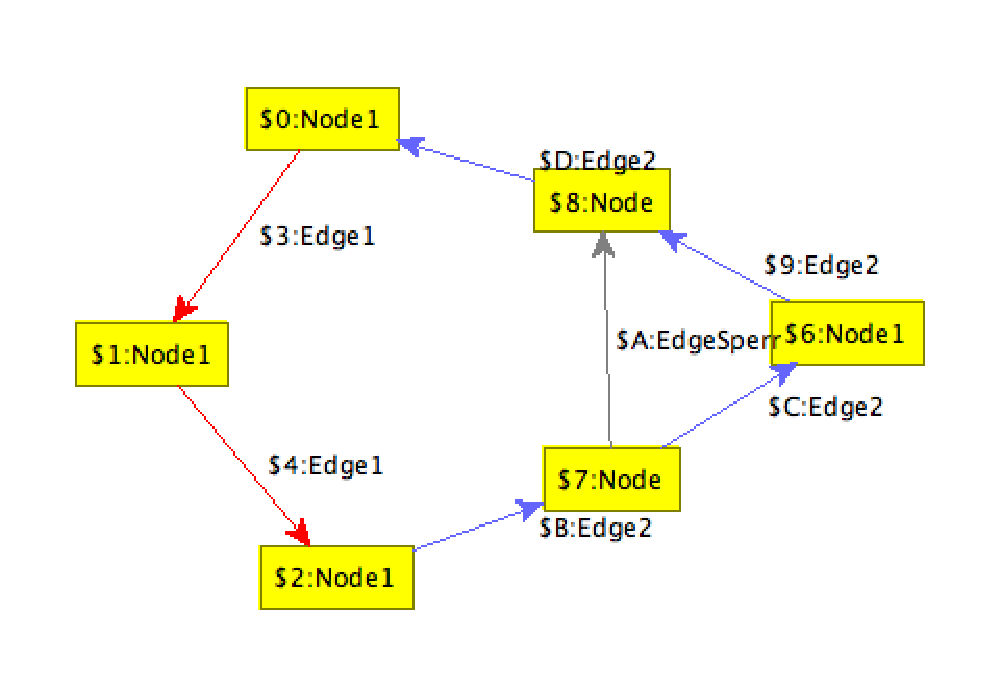
\includegraphics[width=\linewidth]{fig/debug3tra}}
\end{center}
The following table shows the ``break points'' of further debug commands, entered one after another:
\begin{center}
  \begin{tabular}{|l|l|} \hline
    \textbf{Command} & \textbf{Active rule} \\ \hline
    \texttt{s} & \texttt{makeFlake1} \\
    \texttt{o} & \texttt{beautify} \\
    \texttt{s} & \texttt{doNothing} \\
    \texttt{s} & \texttt{beautify} \\ 
    \texttt{u} & \texttt{beautify} \\ 
    \texttt{o} & \texttt{makeFlake2} \\
    \texttt{r} & --- \\ \hline
  \end{tabular}
\end{center}
\end{example}   
\end{figure}

%\subsection{yComp}
%url; yFiles; java app, socket communication with shell debugger
%Find; goto node/edge; b�bbels; 
%relayout; zoom: mousewheel; pane by holding middle mouse
%supported formats; vcg format
%ref to visualization commands, again: hierarchy
%copy some of the stuff from ycomp help?




\chapter{Examples}
\label{anexample}

%%%%%%%%%%%%%%%%%%%%%%%%%%%%%%%%%%%%%%%%%%%%%%%%%%%%%%%%%%%%%%%%%%%%%%%%%%%%%%%%%%%%%%%%%%%%%%%%
\section{Fractals}\indexmain{example}
\label{fractals}
The \GrG\ package ships with samples for fractal generation. We will construct the \indexed{Sierpinski triangle} and the \indexed{Koch snowflake}. They are created by consecutive rule applications starting with the initial host graphs
\begin{center}
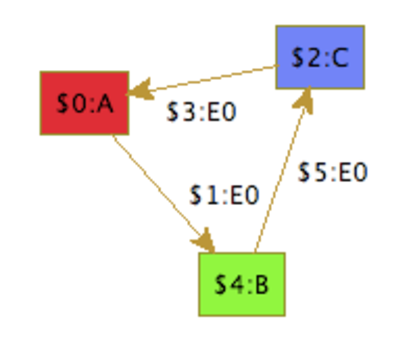
\includegraphics[width=4cm]{fig/startsir}\quad\quad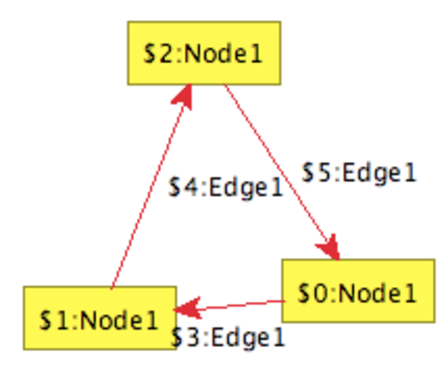
\includegraphics[width=4cm]{fig/startkoch}
\end{center}
for the Sierpinski triangle resp.\ the Koch snowflake. 
First of all we have to compile the model and rule set files. So execute in \GrG's \texttt{bin} directory
\begin{verbatim}
GrGen.exe ..\specs\sierpinski.grg
GrGen.exe ..\specs\snowflake.grg
\end{verbatim}
or
\begin{verbatim}
mono GrGen.exe ../specs/sierpinski.grg
mono GrGen.exe ../specs/snowflake.grg
\end{verbatim}
respectively. If you are on a Unix-like system you have to adjust the path separators of the \GrShell\ scripts. Just edit the first three lines of \texttt{/test/Sierpinski.grs} and \texttt{/test/Snowflake.grs}. And as we have the file \texttt{Sierpinski.grs} already opened, we can increase the number of iterations to get even more beautiful graphs\footnote{Be careful: The running time increases exponentially in the number of iterations.}. Just follow the comments. Be careful when increasing the number of iterations of Koch's snowflake---\yComp's \indexed{layout algorithm} might need some time and attempts to layout it nicely.
We execute the Sierpinski script by
\begin{verbatim}
GrShell.exe ..\test\Sierpinski.grs
\end{verbatim}
or
\begin{verbatim}
mono GrShell.exe ../test/Sierpinski.grs
\end{verbatim}
respectively. Because both of the scripts are using the debug mode, we complete execution by typing \texttt{r}(un). See Section~\ref{grsthings} for further information. The resulting graphs should look like Figures~\ref{figsierp} and~\ref{figsnowflake}.
\begin{figure}[htbp]
  \centering
  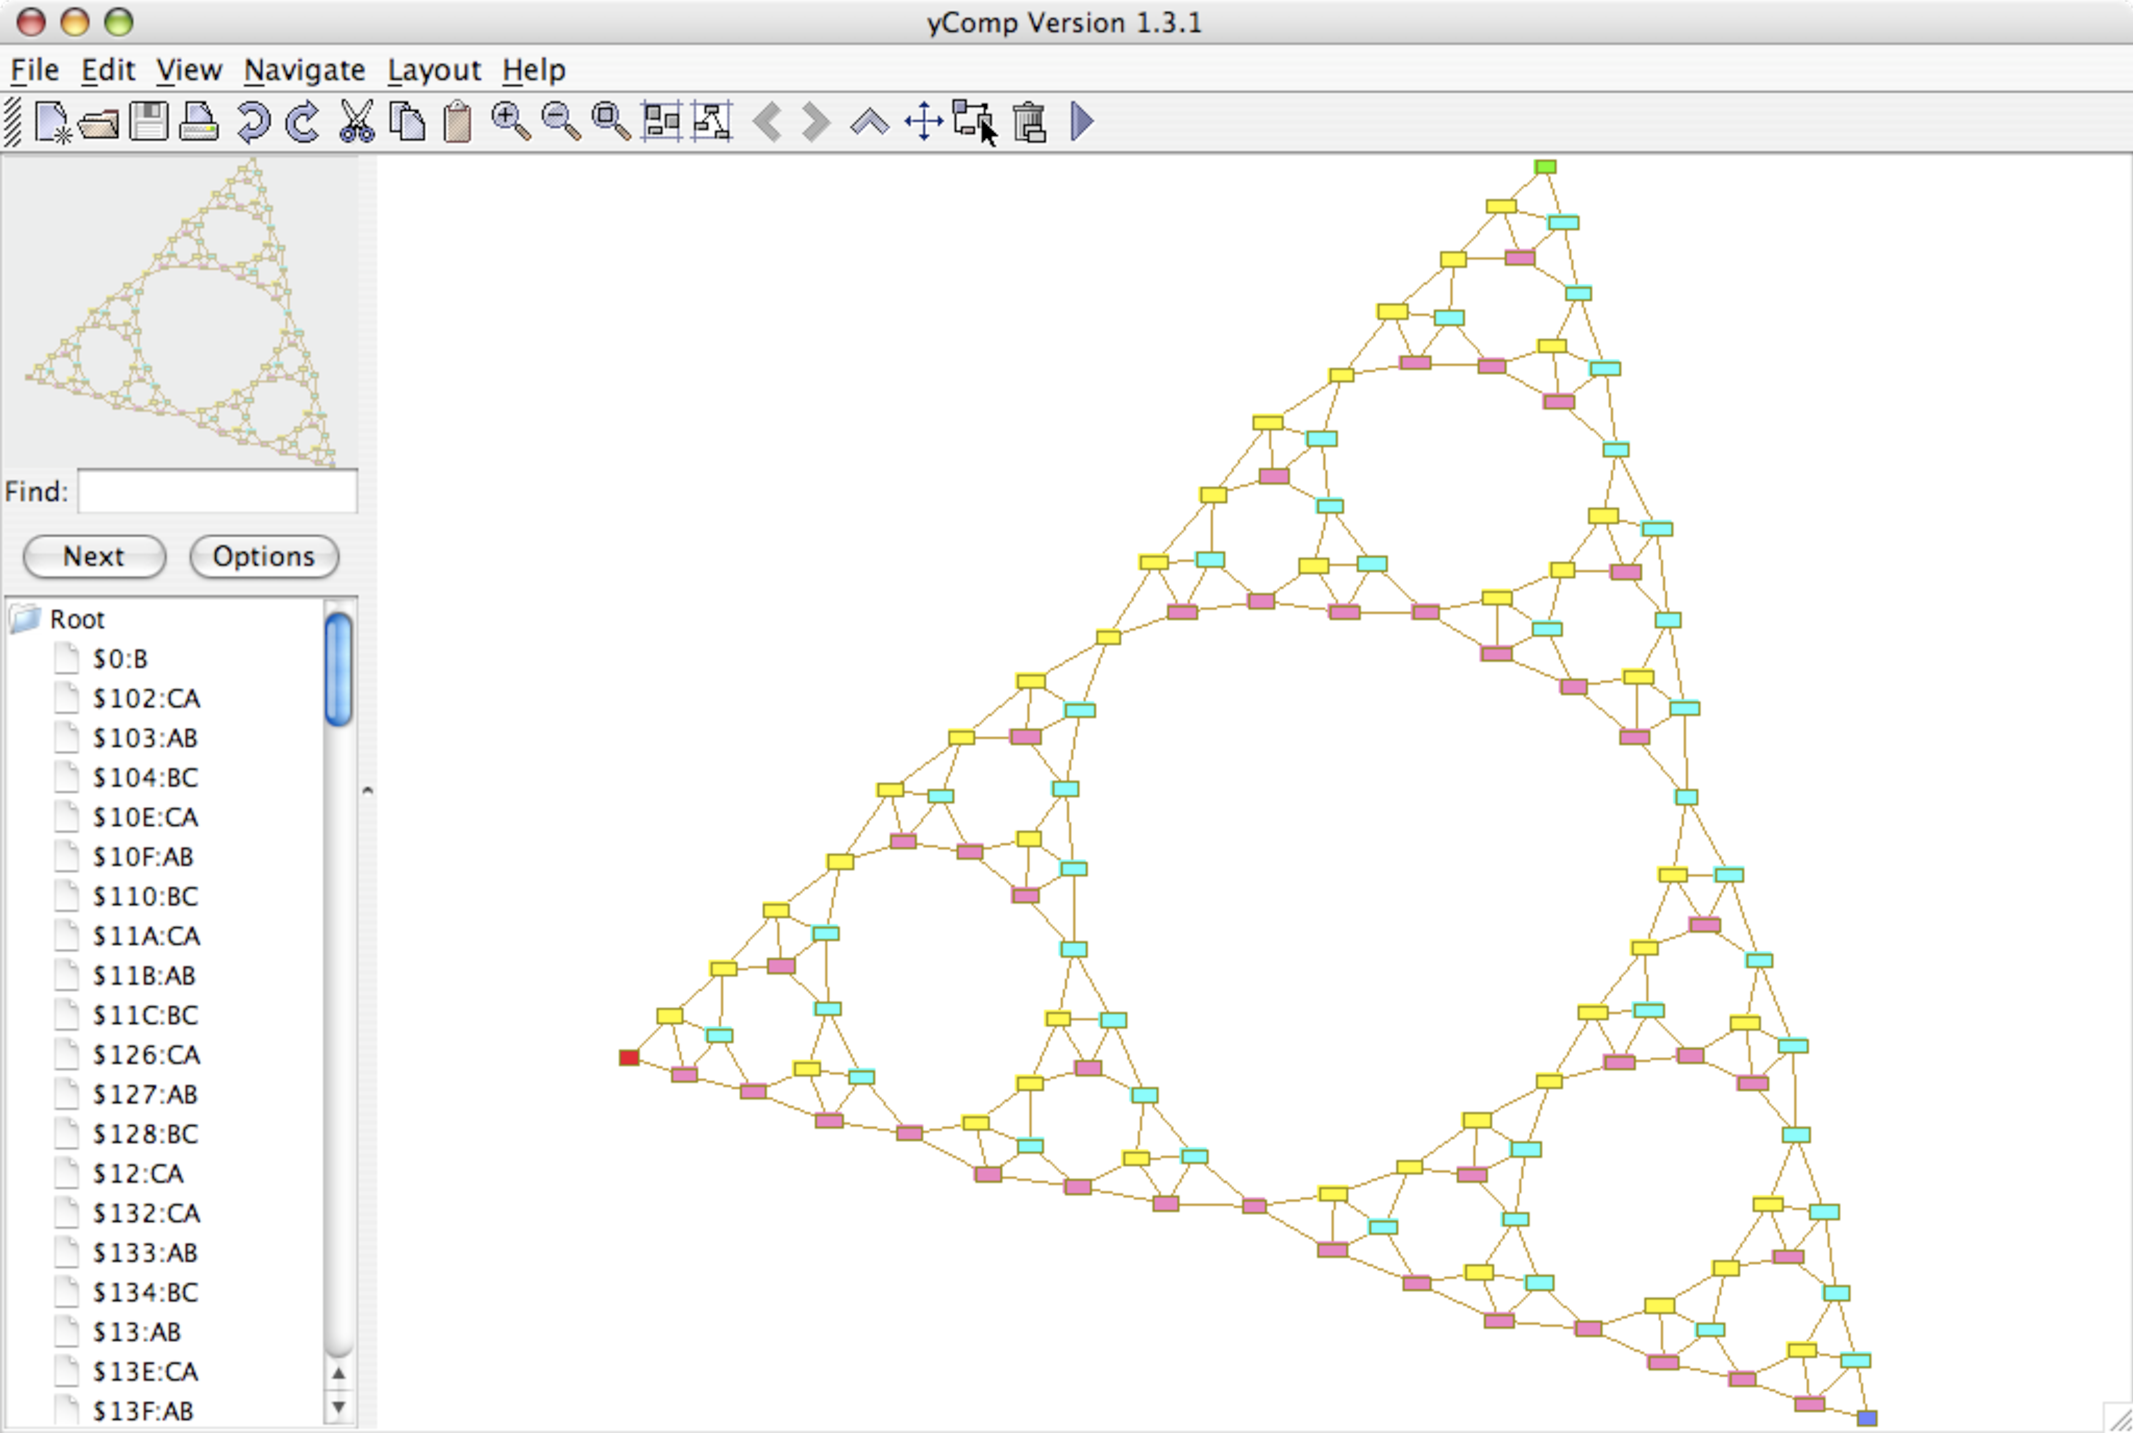
\includegraphics[width=\textwidth]{fig/sierpinski}
  \caption{Sierpinski triangle}
  \label{figsierp}
\end{figure}
\begin{figure}[htbp]
  \centering
  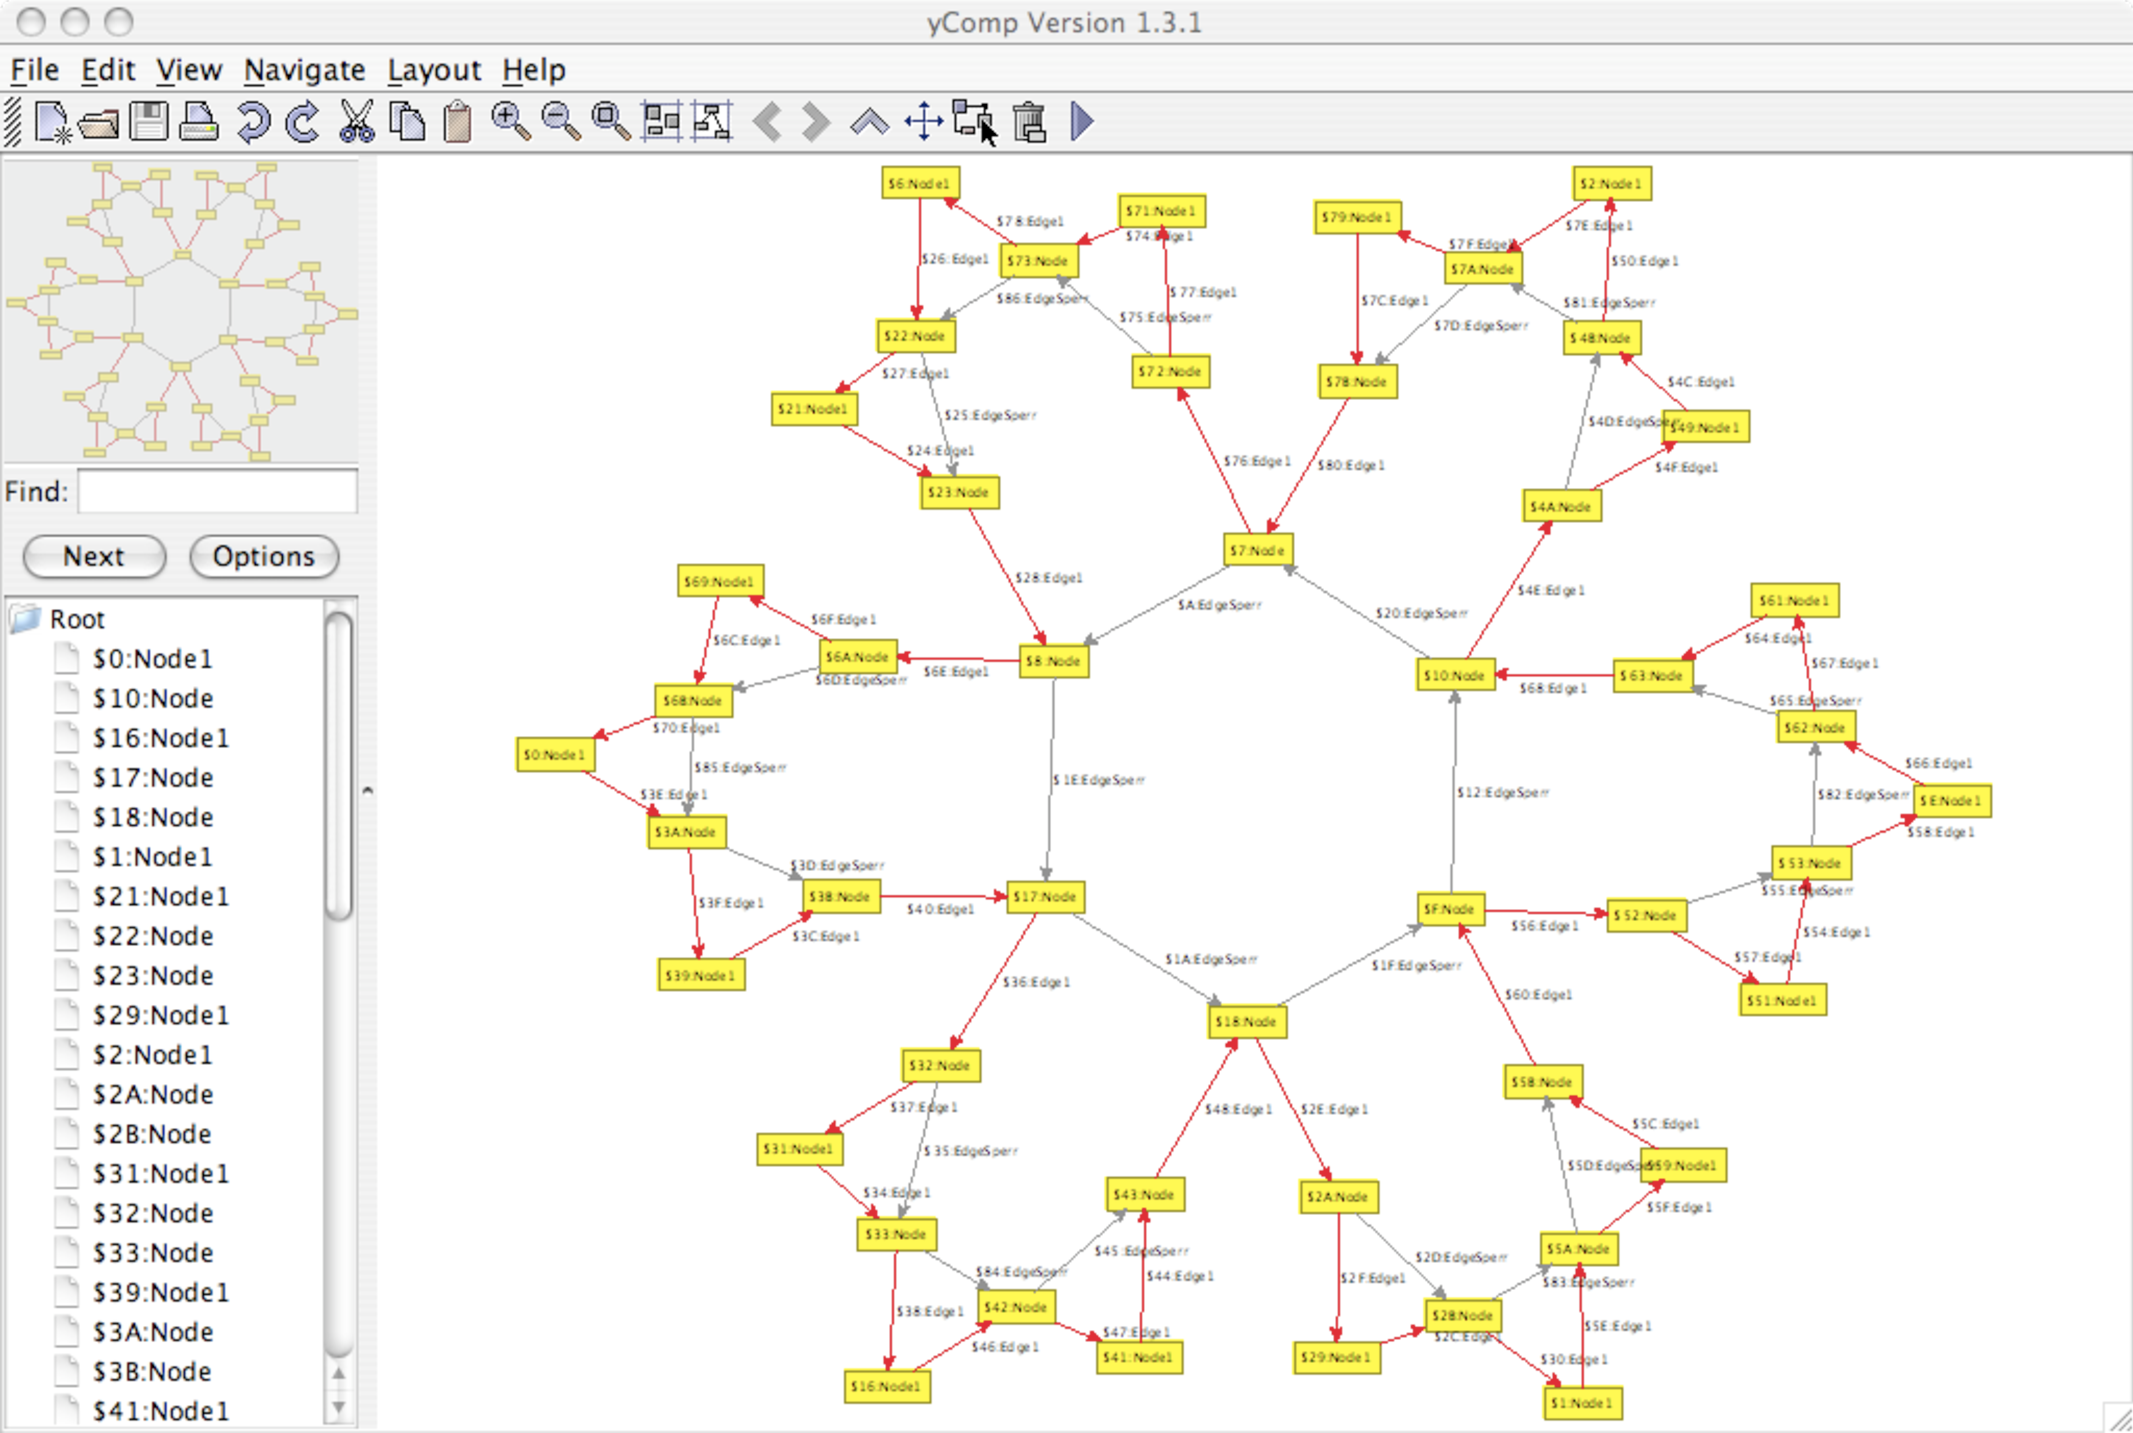
\includegraphics[width=\textwidth]{fig/snowflake}
  \caption{Koch snowflake}
  \label{figsnowflake}
\end{figure}
\vfill\pagebreak


%%%%%%%%%%%%%%%%%%%%%%%%%%%%%%%%%%%%%%%%%%%%%%%%%%%%%%%%%%%%%%%%%%%%%%%%%%%%%%%%%%%%%%%%%%%%%%%%
\section{Busy Beaver}\indexmain{example}
We want \GrG\ to work as hard as a \indexed{busy beaver}~\cite{Kro:07,Dew:84}. Our busy beaver is a Turing machine that has got five states plus a ``halt''-state; it writes 1,471 bars onto the tape and terminates~\cite{MB:00}. So first of all we design a Turing machine as graph model. Besides, this example shows that \GrG\ is \indexed{Turing complete}.

We use the graph model and the rewrite rules to define a general Turing machine. Our approach is to basically draw the machine as a graph. The busy beaver logic is implemented by rule applications in \GrShell.

%-----------------------------------------------------------------------------------------------
\subsection{Graph Model}
The tape will be a chain of \texttt{TapePosition} nodes connected by right edges. A cell value is modeled by a reflexive \texttt{value} edge, attached to a \texttt{TapePosition} node. The leftmost and the rightmost cells (\texttt{TapePosition}) do not have an incoming and outgoing edge respectively. Therefore we have the node constraint $[0:1]$.
\begin{grgen}[firstnumber=last]
node class TapePosition; 
edge class right
  connect TapePosition[0:1] --> TapePosition[0:1];
  
edge class value
  connect TapePosition[1] --> TapePosition[1];  
edge class zero  extends value;
edge class one   extends value;
edge class empty extends value;

\end{grgen}
Furthermore we need states and transitions. 
The machine's current configuration is modeled with a \texttt{RWHead} edge pointing to a \texttt{TapePosition} node. 
\texttt{State} nodes are connected with \texttt{WriteValue} nodes via \texttt{value} edges, a \texttt{moveLeft}/\texttt{moveRight}/\texttt{dontMove} edge leads from a \texttt{WriteValue} node to the next state (cf.~the picture on page \pageref{fig:bbstart}).
\begin{grgen}[firstnumber=last]
node class State;

edge class RWHead;

node class WriteValue;
node class WriteZero extends WriteValue;
node class WriteOne extends WriteValue;
node class WriteEmpty extends WriteValue; 

edge class moveLeft;
edge class moveRight;
edge class dontMove;
\end{grgen}

%-----------------------------------------------------------------------------------------------
\subsection{Rule Set}
Now the rule set: We begin the rule set file \texttt{Turing.grg} with
\begin{grgen}[firstnumber=1] 
using TuringModel;

\end{grgen}
We need rewrite rules for the following steps of the Turing machine:
\begin{enumerate}
  \item Read the value of the current tape cell and select an outgoing edge of the current state.
  \item Write a new value into the current cell, according to the sub type of the \texttt{WriteValue} node.
  \item Move the read-write-head along the tape and select a new state as current state. 
\end{enumerate}
As you can see a transition of the Turing machine is split into two graph rewrite steps: Writing the new value onto the tape and performing the state transition. We need eleven rules: Three rules for each step (for ``zero'', ``one'', and ``empty'') and two rules for extending the tape to the left and the right, respectively.
\begin{grgen}[firstnumber=last] 
rule readZeroRule {
	s:State -h:RWHead-> tp:TapePosition -:zero-> tp;
	s -:zero-> wv:WriteValue;
	modify {
		delete(h);
		wv -:RWHead-> tp;
	}
}      

\end{grgen}
We take the current state \texttt{s} and the current cell \texttt{tp} which is implicitly given by the unique \texttt{RWHead} edge and check whether the cell value is zero. Furthermore we check if the state has a transition for zero. The replacement part deletes the \texttt{RWHead} edge between \texttt{s} and \texttt{tp} and adds it between \texttt{wv} and \texttt{tp}. The remaining rules are analogous:
\begin{grgen}[firstnumber=last] 
rule readOneRule {
	s:State -h:RWHead-> tp:TapePosition -:one-> tp;
	s -:one-> wv:WriteValue;
	modify {
		delete(h);
		wv -:RWHead-> tp;
	}
}

rule readEmptyRule {
	s:State -h:RWHead-> tp:TapePosition -:empty-> tp;
	s -:empty-> wv:WriteValue;
	modify {
		delete(h);
		wv -:RWHead-> tp;
	}
}

rule writeZeroRule {
	wv:WriteZero -rw:RWHead-> tp:TapePosition -:value-> tp;
	replace {
		wv -rw-> tp -:zero-> tp;
	}	
}

rule writeOneRule {
	wv:WriteOne -rw:RWHead-> tp:TapePosition -:value-> tp;
	replace {
		wv -rw-> tp -:one-> tp;
	}	
}

rule writeEmptyRule {
	wv:WriteEmpty -rw:RWHead-> tp:TapePosition -:value-> tp;
	replace {
		wv -rw-> tp -:empty-> tp;
	}	
}

rule moveLeftRule {
	wv:WriteValue -:moveLeft-> s:State;
	wv -h:RWHead-> tp:TapePosition <-r:right- ltp:TapePosition;
	modify {
		delete(h);
		s -:RWHead-> ltp;
	}
}

rule moveRightRule {
	wv:WriteValue -:moveRight-> s:State;
	wv -h:RWHead-> tp:TapePosition -r:right-> rtp:TapePosition;
	modify {
		delete(h);
		s -:RWHead-> rtp;
	}
}

rule dontMoveRule {
	wv:WriteValue -:dontMove-> s:State;
	wv -h:RWHead-> tp:TapePosition;
	modify {
		delete(h);
		s -:RWHead-> tp;
	}
}

rule ensureMoveLeftValidRule {
	wv:WriteValue -:moveLeft-> :State;
	wv -:RWHead-> tp:TapePosition;
	negative {
		tp <-:right-;
	}
	modify {
		tp <-:right- ltp:TapePosition -:empty-> ltp;
	}
}

rule ensureMoveRightValidRule {
	wv:WriteValue -:moveRight-> :State;
	wv -:RWHead-> tp:TapePosition;
	negative {
		tp -:right->;
	}
	modify {
		tp -:right-> rtp:TapePosition -:empty-> rtp;
	}
}
\end{grgen}
Have a look at the negative conditions within the \texttt{ensureMove\dots} rules. They ensure that the current cell is indeed at the end of the tape: An edge to a right/left neighboring cell must not exist. Now don't forget to compile your model and the rule set with \texttt{GrGen.exe} (see Section~\ref{fractals}).

%-----------------------------------------------------------------------------------------------
\subsection{Rule Execution with \GrShell}

Finally we construct the busy beaver and let it work with \GrShell. The following script starts with building the Turing machine that is modeling the six states with their transitions in our Turing machine model:
\begin{grshell}[firstnumber=1] 
select backend "../bin/lgspBackend.dll"
new graph "../lib/lgsp-TuringModel.dll" "Busy Beaver"
select actions "../lib/lgsp-TuringActions.dll"

# Initialize tape
new tp:TapePosition($="Startposition")
new tp -:empty-> tp

# States
new sA:State($="A")
new sB:State($="B")
new sC:State($="C")
new sD:State($="D")
new sE:State($="E")
new sH:State($ = "Halt")

new sA -:RWHead-> tp

# Transitions: three lines per state and input symbol for
#   - updating cell value
#   - moving read-write-head
# respectively

new sA_0: WriteOne
new sA -:empty-> sA_0
new sA_0 -:moveLeft-> sB

new sA_1: WriteOne
new sA -:one-> sA_1
new sA_1 -:moveLeft-> sD

new sB_0: WriteOne
new sB -:empty-> sB_0
new sB_0 -:moveRight-> sC

new sB_1: WriteEmpty
new sB -:one-> sB_1
new sB_1 -:moveRight-> sE

new sC_0: WriteEmpty
new sC -:empty-> sC_0
new sC_0 -:moveLeft-> sA

new sC_1: WriteEmpty
new sC -:one-> sC_1
new sC_1 -:moveRight-> sB

new sD_0: WriteOne
new sD -:empty-> sD_0
new sD_0 -:moveLeft->sE

new sD_1: WriteOne
new sD -:one-> sD_1
new sD_1 -:moveLeft-> sH

new sE_0: WriteOne
new sE -:empty-> sE_0
new sE_0 -:moveRight-> sC

new sE_1: WriteOne
new sE -:one-> sE_1
new sE_1 -:moveLeft-> sC

\end{grshell}
\quad\\Our busy beaver looks like this:\label{fig:bbstart}
\begin{center}
  \fbox{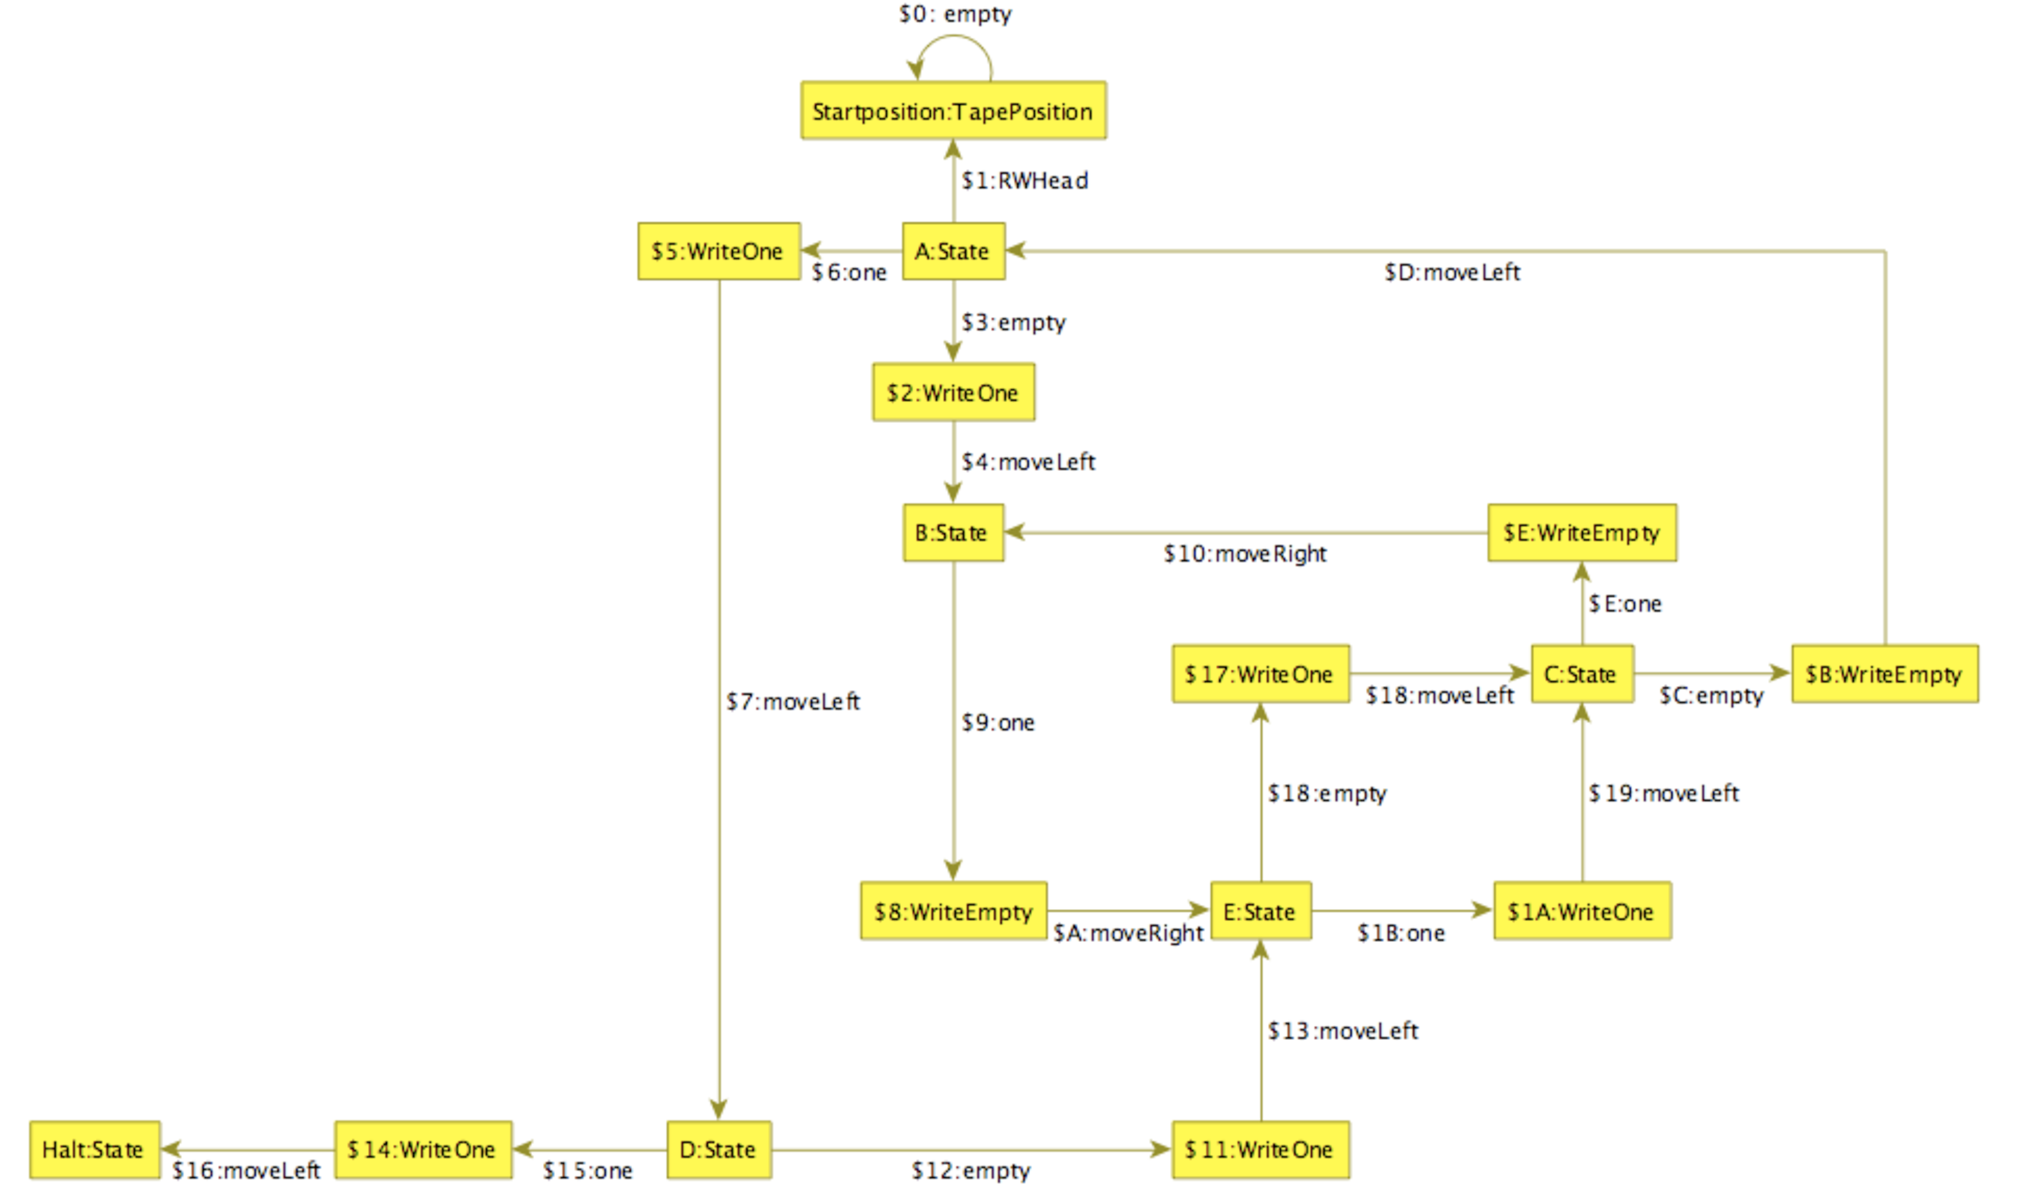
\includegraphics[width=\linewidth-2\fboxsep-2\fboxrule]{fig/bbstart}}
\end{center}

We have an initial host graph now. The graph rewrite sequence is quite straight forward and generic to the Turing graph model. Note that for each state the ``\texttt{\dots Empty\dots} | \texttt{\dots One\dots}'' selection is unambiguous.
%\pagebreak %HACK
\begin{grshell}[firstnumber=last]
  xgrs ((readOneRule | readEmptyRule) & (writeOneRule | writeEmptyRule) & (ensureMoveLeftValidRule | ensureMoveRightValidRule) & (moveLeftRule | moveRightRule))[32]

\end{grshell}
\quad\\We interrupt the machine after 32 iterations and look at the result so far:
\begin{center}
  \fbox{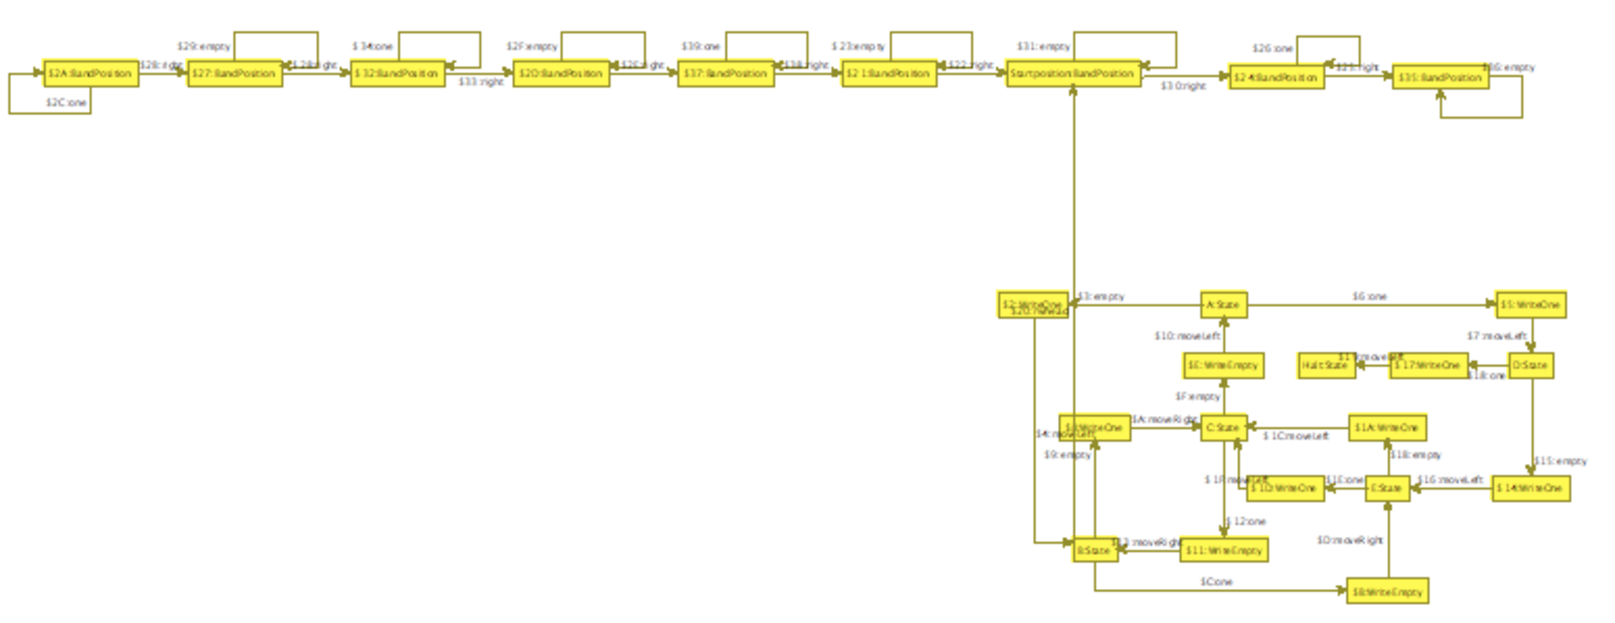
\includegraphics[width=\linewidth-2\fboxsep-2\fboxrule]{fig/bbmiddle}}
\end{center}
In order to improve the performance we generate better \indexed{search plan}s. This is a crucial step for execution time: With the initial search plans the beaver runs for 1 minute and 30 seconds. With improved search plans after the first 32 steps he takes about 8.5 seconds\footnote{On a Pentium 4, 3.2Ghz, with 2GiB RAM.}.
\begin{grshell}[firstnumber=last]
custom graph analyze_graph
custom actions gen_searchplan readOneRule readEmptyRule writeOneRule writeEmptyRule ensureMoveLeftValidRule ensureMoveRightValidRule moveLeftRule moveRightRule

\end{grshell}

Let the beaver run:
\begin{grshell}[firstnumber=last]
  xgrs ((readOneRule | readEmptyRule) & (writeOneRule | writeEmptyRule) & (ensureMoveLeftValidRule | ensureMoveRightValidRule) & (moveLeftRule | moveRightRule))*
\end{grshell}




\chapter{Application Programming Interface}\indexmainsee{application programming interface}{API} \indexmain{API}
\label{cha:api}

This chapter describes the Application Programming Interface of \GrG, i.e. of the system runtime - the LibGr - and of the assemblies generated from the model and rule specifications.
We'll have a look at
\begin{itemize}
\item the interface to the graph and model
\item the interface to the rules and matches
\item the interface of the graph processing environment
\item the porter module for importing and exporting of graphs and miscellaneous stuff
\item implementing external class and function declarations
\item implementing external match filter and external sequence declarations
\item events fired when the graph is changed
\item events fired during action execution
\end{itemize}

\noindent From the input file \texttt{Foo.grg} \texttt{grgen.exe} generates the output files \texttt{FooModel.cs} for the model and \texttt{FooActions.cs} for the actions,
\begin{itemize}
\item defining the exact interface, 
\item implementing the exact interface with generated code and code from the lgsp backend, i.e. entities from \texttt{de.unika.ipd.grGen.lgsp} available from lgspBackend.dll, 
\item and implementing the generic interface from \texttt{de.unika.ipd.grGen.libGr} using the entities mentioned in both points above.
\end{itemize}

\noindent This generative approach bears a great deal of the responsibility for the high execution speed of GrGen.NET, but it comes at the price of flexibility: you can't extend the rule set at runtime with new rules.
What you can do at runtime on the other hand is to generate a new rule set file, apply the compiler, and dynamically link the resulting assemblies/dlls.

When working with the API, you could reference the generated binary dlls in your project, in the same way as you have to reference the \texttt{libGr.dll} and \texttt{lgspBackend.dll}.
For easier debugging though, especially when you are integrating the generated code with own extensions (as described in chapter \ref{chapextensions}), it is recommended to directly include the source code generated (which is thrown away normally after it was compiled into the assemblies lgsp-FooModel.dll and lgsp-FooActions.dll).
For this, use the \texttt{-keep} option when you call \texttt{grgen.exe}, and include the model and the actions file (excluding the intermediate actions file) directly as C\# source code files.

The matcher code generated contains the initial, static search plans.
When you analyze the graph at runtime and generate new matchers, see section \ref{custom} for more on this, you can request the dumping of the source code of the improved matchers.
The custom commands are available at API level via the \texttt{Custom} operation of the \texttt{IGraph} interface for the graph commands and the \texttt{Custom} operation of the \texttt{BaseActions} class for the actions commands, just handing in the same parameters as otherwise specified on the command line.
If the intended workflow of ``i) loading a typical graph or doing a warm-up run creating a typical graph, ii) analyzing that graph, iii) compiling new matchers which are better suited to the graph'' is not easily achievable, or you want to start with the optimized matchers straight from the beginning, you may copy and paste the dumped dynamic matchers of an example run to the existing static code. 
But this is only a last resort, as the price is that your manual editing is overwritten again with the static search plans at the next time you call \texttt{grgen}.


%%%%%%%%%%%%%%%%%%%%%%%%%%%%%%%%%%%%%%%%%%%%%%%%%%%%%%%%%%%%%%%%%%%%%%%%%%%%%%%%%%%%%%%%%%%%%%%%
\section{Interface to the Host Graph}

The generated file \texttt{FooModel.cs} opens the namespace \texttt{de.unika.ipd.grGen.Model\_Foo} containing all the generated entities.
It contains for every node or edge class \texttt{Bar} an interface \texttt{IBar}, which offers C\# properties giving access to the attributes, and is inheriting in the same way as specified in the model file.
This builds the exact interface of the model, it is implemented by a sealed class \texttt{Bar} with generated code and with code from the lgsp backend.
Furtheron the namespace contains a model class \texttt{FooGraphModel} implementing the interface \texttt{de.unika.ipd.grGen.libGr.IGraphModel},
which supports iteration over the entities defined in the model using further, generic(i.e. inexact) interfaces from libGr.
Finally, the namespace contains a class \texttt{FooGraph} which defines an \texttt{LGSPGraph} of a model equivalent to \texttt{FooGraphModel}; 
it contains convenience functions to easily create nodes and edges of exact type in the graph.
In addition, a class \texttt{FooNamedGraph} is available, which defines an \texttt{LGSPNamedGraph} of a model equivalent to \texttt{FooGraphModel}; 
the named graph offers persistent names \ref{persistentex} for all its graph elements, otherwise it is identical to an \texttt{LGSPGraph}.
The naming requires about the same memory as an unnamed graph, but under normal circumstances the named graph is the recommended one to use (and is the one which will be used if employed by the shell).

\begin{note}
If you want to use the type-safe interface, use the interface \texttt{IBar}, and the \texttt{CreateNodeBar}-methods of \texttt{FooGraph} or the \texttt{CreateNode}-method of \texttt{Bar}.
If you want to use the generic interface, your entry point is the \texttt{IGraphModel}, with \texttt{INodeModel.GetType("Bar")} returning a \texttt{NodeType}, used in \texttt{IGraph.AddNode(NodeType)} returning an \texttt{INode}.
\end{note}


%%%%%%%%%%%%%%%%%%%%%%%%%%%%%%%%%%%%%%%%%%%%%%%%%%%%%%%%%%%%%%%%%%%%%%%%%%%%%%%%%%%%%%%%%%%%%%%%
\section{Interface to the Rules}

The generated file \texttt{FooActions.cs} opens the \texttt{namespace de.unika.ipd.grGen.Action\_Foo} containing all the generated entities.
It contains for every rule or test \texttt{bar}
\begin{itemize}
\item a class \texttt{Rule\_bar} inheriting from \texttt{de.unika.ipd.grGen.lgsp.LGSPRulePattern}, which contains
the exact match interface \texttt{IMatch\_bar} which defines how a match of the rule looks like,
extending the generic rule-unspecific \texttt{IMatch} interface.
Have a look at section \ref{sub:extflt} for an extended introduction to the matches interfaces. 
Furtheron there are (but meant only for internal use): a match class \texttt{Match\_bar} implementing the exact and inexact interface,
a description of the pattern to match, and the modify methods doing the rewriting.
\item an exact action interface \texttt{IAction\_bar} which contains the methods:
  \begin{itemize}
  \item \texttt{Match}, to match the pattern in the host graph,
     with in-parameters corresponding to the in-parameters of the rule (name and type),
	 returning matches of the exact type \texttt{Rule\_bar.IMatch\_bar}.
  \item \texttt{Modify}, to modify a given match according to the rewrite specification,
     with out-parameters corresponding to the out-parameters of the rule.
  \item \texttt{Apply}, to match and modify the found match,
     with in-parameters corresponding to the in-parameters of the rule,
     and with ref-parameters corresponding to the out-parameters of the rule.
  \end{itemize}
  Furtheron there is (but meant only for internal use) the class \texttt{Action\_bar} implementing the exact action interface as well as the generic \texttt{IAction} interface from libGr;
  it contains the generated matcher code searching for the patterns.
\end{itemize}

Moreover the namespace contains an action class \texttt{FooActions}
implementing the abstract class \texttt{de.unika.ipd.grGen.libGr.BaseActions} (in fact \texttt{de.unika.ipd.grGen.lgsp.LGSPActions}),
which supports iteration over the entities defined in the actions using further, generic(i.e. inexact) interfaces from libGr.
Additionally, at runtime it contains the instances of the actions singletons,
as member \texttt{bar} of the exact type \texttt{IAction\_bar}.
\begin{note}
If you want to use the type-safe interface, your entry point is the member \texttt{bar} of type \texttt{IAction\_bar} from \texttt{FooActions} (or \texttt{Action\_bar.Instance}).
Actions are used with named parameters of exact types.
If you want to use the generic interface, your entry point is the method \texttt{GetAction("bar")} of the interface \texttt{BaseActions} implemented by \texttt{FooActions} returning an \texttt{IAction}.
Actions are used with \texttt{object}-arrays for parameter passing.
\end{note}

\begin{note}
The old generic interface of string names and entities of node-,edge-, and object-type is implemented with the new interface of exactly typed, named entities.
Thus you will receive runtime exceptions when doing operations which are not type-safe with the generic interface, in contrast to \GrG\ $<$ v2.5.
If you need the flexibility of the old input parameters semantics of silently failing rule application on a wrong type,
you must declare it explicitly with the syntax \verb#r(x:ExactType<InexactType>)#;
then the rule parameter in the exact interface will be of type \texttt{InexactType}.
\end{note}

\begin{example}\label{ex:api1}
Normally you want to use the type-safe interface of the generated code as it is much more convenient.
Only if your application must get along with models and actions unknown before it is compiled you have to fall back to the generic interface.
An extensive example showing how to cope with the latter is shipped with \GrG\ in form of the GrShell.
Here we'll show a short example on how to use \GrG\ with the type-safe API; 
further examples are given in the examples-api folder of the \GrG-distribution.

We'll start with including the namespaces of the libGr and the lgsp backend shipped with \GrG\,
plus the namespaces of our actions and models, generated from \texttt{Foo.grg}.
\begin{verbatim}
using de.unika.ipd.grGen.libGr;
using de.unika.ipd.grGen.lgsp;
using de.unika.ipd.grGen.Action_Foo;
using de.unika.ipd.grGen.Model_Foo;
\end{verbatim}

Then we create a graph with model bound at generation time and create actions to operate on this graph.
Afterwards we create a single node of type \texttt{Bar} in the graph and save it to the variable \texttt{b}.
Finally we apply the action \texttt{bar(Bar x) : (Bar)} to the graph with \texttt{b} as input receiving the output as well.
The rule is taken from the actions via the member named as the action.
\begin{verbatim}
FooGraph graph = new FooGraph();
FooActions actions = new FooActions(graph);
Bar b = graph.CreateNodeBar();
actions.bar.Apply(graph, b, ref b); // input of type Bar, output of type Bar
\end{verbatim}

We could create a named graph instead offering persistent names for its graph elements:
\begin{verbatim}
FooNamedGraph graph = new FooNamedGraph();
\end{verbatim}
\end{example}

\begin{example}
This is an example doing mostly the same as the previous example \ref{ex:api1}, in a slightly more complicated way allowing for more control.
Here we create the model separate from the graph, then the graph with a model not bound at generation time.
We create the actions to apply on the graph, and a single node of type \texttt{Bar} in the graph, which we assign again to a variable \texttt{b}.
Then we get the action from the actions and save it to an action variable \texttt{bar};
afterwards we use the action for finding all available matches of \texttt{bar} with input \texttt{b} -- which is different from the first version -- and remember the found matches in the matches variable with its exact type.
Finally we take the first match from the matches and execute the rewrite with it.
We could have inspected the nodes and edges of the match or their attributes before (using element names prefixed with \texttt{node\_/edge\_} or attribute names to get exactly typed entities). 
\begin{verbatim}
IGraphModel model = new FooGraphModel();
LGSPGraph graph = new LGSPGraph(model);
FooActions actions = new FooActions(graph);
Bar b = Bar.CreateNode(graph);
IAction_bar bar = Action_bar.Instance;
IMatchesExact<Rule_bar.IMatch_bar> matches = bar.Match(graph, 0, b);
bar.Modify(graph, matches.First);
\end{verbatim}

We could create a named graph instead offering persistent names for its graph elements:
\begin{verbatim}
LGSPGraph graph = new LGSPNamedGraph(model);
\end{verbatim}
\end{example}

%%%%%%%%%%%%%%%%%%%%%%%%%%%%%%%%%%%%%%%%%%%%%%%%%%%%%%%%%%%%%%%%%%%%%%%%%%%%%%%%%%%%%%%%%%%%%%%%
\section{Interface of the Graph Processing Environment}

The interface \texttt{IGraphProcessingEnvironment} implemented by the \texttt{LGSPGraphProcessing\-Environment} class offers all the additional functionality of \GrG~exceeding what is offered by the graph and the actions.
It is constructed as \texttt{LGSPGraphProcessingEnvironment} given the graph and the actions.
It offers execution of the sequences and variable handling, combining actions into transformations
(the former regarding control flow, the latter regarding data flow).

\begin{example}\label{ex:procenv}
For all but the simplest transformations you'll end up constructing a graph processing environment from the graph and the actions constructed until now, executing a graph rewrite sequence on the graph processing environment:
\begin{verbatim}
LGSPGraphProcessingEnvironment procEnv = 
    new LGSPGraphProcessingEnvironment(graph, actions);
procEnv.ApplyGraphRewriteSequence("<(::x)=foo && (::y)=bar(::x) | bla(::y)>");
\end{verbatim}
\end{example}

In addition to sequences and variables handling, the graph processing environment offers driver or helper objects for transaction management, deferred sequence execution, graph change recording, and emitting.
The most important of these is the transaction manager which is utilized when \GrG~ is used for crawling through a search space or for enumerating a state space, see section \ref{sec:extctrl}.
The operations mentioned there are implemented by calling the function given in example \ref{ex:transman}.

\begin{example}\label{ex:transman}
\begin{verbatim}
LGSPGraphProcessingEnvironment procEnv = ...;
ITransactionManager tm = procEnv.TransactionManager;
public interface ITransactionManager
{
    int Start();
    void Pause();
    void Resume();
    void Commit(int transactionID);
    void Rollback(int transactionID);
}
\end{verbatim}
\end{example}

The \texttt{Start} starts a transaction and returns its id; it may be called multiple times returning different ids for the then nested transactions (i.e. a failing outer one rolls back the changes of an inner transaction which succeeded).
Changes to the graph are recorded thereafter into an undo log, unless a \texttt{Pause} was called not yet followed by a \texttt{Resume}.
When the changes of interest were carried out the transaction identified by its id is either \texttt{Commit}ed, which causes the changes recorded since the corresponding \texttt{Start} to stay in the graph, or rolled back by calling \texttt{Rollback}, in that case all the changes recorded since the corresponding \texttt{Start} are undone.

%%%%%%%%%%%%%%%%%%%%%%%%%%%%%%%%%%%%%%%%%%%%%%%%%%%%%%%%%%%%%%%%%%%%%%%%%%%%%%%%%%%%%%%%%%%%%%%%
\section{Import/Export and Miscellaneous Stuff}\label{sub:imexport}\indexmain{import}\indexmain{export}

GrGen natively supports the following formats:
\begin{description}
  \item[GRS/GRSI] Reduced GrShell script files (graph only, model from \texttt{.gm}; a very limited version of the normal \texttt{.grs}. The recommended standard format.)
  \item[GXL] Graph eXchange Language (\texttt{.gxl}-files, see \url{http://www.gupro.de/GXL/})
  \item[ECORE/XMI] Ecore(\texttt{.ecore}) model files and XMI(\texttt{.xmi}) graph file. Import only, export must be programmed with \texttt{emit}-statements. In an intermediate step, a \texttt{.gm} file is generated for the model.
    \item[GRG] Writes a GrGen rule file containing one rule with an empty pattern and a large rewrite part. Export only \footnote{Original German Pisswasser, for export only :)}, not for normal use.
\end{description}

While both GRS and GXL importers expect one file
(the GXL importer allows to specify a model override, see GrShell import, Note \ref{shellgxlimport}),
the EMF/ECORE importer expects first one or more \texttt{.ecore} files
and following optionally a \texttt{.xmi} files and/or a \texttt{.grg} file (cf. Note \ref{shellecoreexport}). 
To use additional custom graph models you should supply an own \texttt{.grg}
file which may be based on the automatically generated \texttt{.grg} file, if none was
supplied (see the Program-Comprehension example in \texttt{examples/ProgramComprehension-GraBaTs09}).

To import a graph model and/or a graph instance you can use \texttt{Porter.Import()} from the libGr API (the GrShell command \texttt{import} is mapped to it)
The file format is determined by the file extensions.
To export a graph instance you can use \texttt{Porter.Export()} from the libGr API (the GrShell command \texttt{export} is mapped to it).
For an example of how to use the importer/exporter on API level see \texttt{examples-api/JavaProgramGraphsExample/JavaProgramGraphs\-Example.cs}

The GRS(I) importer returns an \texttt{INamedGraph};
if you don't need the persistent names, get rid of them by casting to the \texttt{LGSPNamedGraph} implementing the interface, (copy-)constructing a \texttt{LGSPGraph} from it, and forgetting any references to the named graph.
Please be aware that naming is rather expensive:
A \texttt{LGSPNamedGraph} supplying the name to element and element to name mappings normally uses up about twice the amount of memory of the \texttt{LGSPGraph} defining the graph alone (but is worth is most often).

There are further examples available in the \texttt{examples-api} folder of the \GrG-distribution:
\begin{itemize} 
\item How to use the graph rewrite sequences offered by the libGr on API level is shown in\\
\texttt{examples-api/BusyBeaverExample/BusyBeaverExample.cs}.\\
But normally you want to use your favourite .NET programming language for control together with the type-safe interface when working on API level.
\item How to use the old and new interface for accessing a match on API level is shown in\\
\texttt{examples-api/ProgramGraphsExample/ProgramGraphsExample.cs}.
\item How to use the visited\label{apiallocvisitflag} flags on API level is shown in\\
\texttt{examples-api/VisitedExample/VisitedExample.cs}.
\item How to analyze the graph and generate (hopefully) better performing matchers based on this information is shown in\\
\texttt{examples-api/BusyBeaverExample/BusyBeaverExample.cs}.
\item How to compile a \texttt{.grg}-specification at runtime and dump a graph for visualization in \texttt{.vcg} format on the API level is shown in\\
\texttt{examples-api/HelloMutex/HelloMutex.cs}.
\item How to access the annotations at API level is shown in\\
\texttt{examples-api/MutexDirectExample/MutexDirectExample.cs}.
\item How to communicate with yComp on the API level (from your own code) is shown in\\
\texttt{examples-api/YCompExample/YCompExample.cs}.
\end{itemize}

\begin{warning}
While C\# allows input arguments values to be of a subtype of the declared interface parameter type (OO), 
it requires that the argument variables for the \texttt{out} parameters are of exactly the type declared (non-OO).
Although a variable of a supertype would be fully sufficient -- the variable is only assigned.
So for \texttt{node class Bla extends Bar;} and action \texttt{bar(Bar x) : (Bla)} from the rules file rules \texttt{Foo.grg}
we can't use a desired target variable of type \texttt{Bar} as \texttt{out}-argument,
but are forced to introduce a temporary variable of type \texttt{Bla}
and assign this variable to the desired target variable after the call.
\begin{csharplet}
using de.unika.ipd.grGen.libGr;
using de.unika.ipd.grGen.lgsp;
using de.unika.ipd.grGen.Action_Foo;
using de.unika.ipd.grGen.Model_Foo;
FooGraph graph = new FooGraph();
FooActions actions = new FooActions(graph);
Bar b = graph.CreateNodeBar();
IMatchesExact<Rule_bar.IMatch_bar> matches = actions.bar.Match(graph, 1, b);
//actions.bar.Modify(graph, matches.First, out b); // wont work, needed:
Bla bla = null; 
actions.bar.Modify(graph, matches.First, out bla);
b = bla;
\end{csharplet}
\end{warning}


%%%%%%%%%%%%%%%%%%%%%%%%%%%%%%%%%%%%%%%%%%%%%%%%%%%%%%%%%%%%%%%%%%%%%%%%%%%%%%%%%%%%%%%%%%%%%%%%
\section{External Class, Function and Procedure Implementation}\label{sub:extclsfctimpl}\indexmain{external class implementation}\indexmain{external function implementation}\indexmain{external procedure implementation}

For a model file \texttt{Foo} which contains external functions (cf. \ref{sub:extfct}) and/or classes (cf. \ref{sub:extcls}), \GrG~generates a file \texttt{FooModelExternalFunctions.cs} located besides the model and rule files, which contains
\begin{itemize}
	\item within the model namespace public partial classes named as given in the external class declaration,
inherting from each other as stated in the external class declarations.
	\item within the \texttt{de.unika.ipd.grGen.expression} namespace a public partial class named \texttt{ExternalFunctions} with a body of comments giving the expected function and procedure prototypes.
\end{itemize}

\noindent The partial classes are empty, you must implement them in a file named \texttt{FooModelExternal\-FunctionsImpl.cs} located in the folder of the \texttt{FooModelExternalFunctions.cs} file by
\begin{itemize}
	\item fleshing out the partial classes skeletons with attributes containing data of interest and maybe helper methods
	\item fleshing out the \texttt{ExternalFunctions} partial class skeleton with the functions you declared in the external function declarations, obeying the function signatures as specified; here you can access the now know attributes or methods of the external classes, or do complicated custom computations or graph querying with the values you receive from a function call.
	\item fleshing out the \texttt{ExternalProcedures} partial class skeleton with the procedures you declared in the external procedure declarations, obeying the procedure signatures as specified; here you can access the now know attributes or methods of the external classes, or do complicated custom computations or graph manipulations with the values you receive from a procedure call.
\end{itemize}

\noindent Don't forget that the source code file \texttt{FooModelExternalFunctionsImpl.cs} is an integral part of your \GrG~graph transformation project, in contrast to the other C\# files generated (and overwritten) for you.
In \texttt{examples/ExternalAttributeEvaluationExample} and \texttt{examples-api/ExternalAttributeEvaluationExample}
you find a fabricated example showing how to use the external classes and functions.

When you use third-party assemblies in your source code you must inform GrGen.NET about them so references to them are included into the assembly generated; this can be done with the \texttt{-r} parameter when calling \texttt{grgen.exe} directly (cf. \ref{grgenoptions}) or with the \texttt{new} command configurations available in GrShell (cf. \ref{graphcommands}). Using the \texttt{keepdebug} configuration of the \texttt{new} command is recommended as it allows for easier debugging.


%%%%%%%%%%%%%%%%%%%%%%%%%%%%%%%%%%%%%%%%%%%%%%%%%%%%%%%%%%%%%%%%%%%%%%%%%%%%%%%%%%%%%%%%%%%%%%%%
\section{External Filter and Sequence Implementation}\label{sub:extfltseqimpl}\indexmain{external match filter implementation}\indexmain{external sequence implementation}

For an actions file \texttt{Bar} which contains match filter declarations (cf. \ref{sub:extflt}) and/or external sequence declarations (\ref{sub:extseq}), \GrG~generates a file \texttt{BarActionsExternalFunctions.cs} located besides the model and rule files, which contains within the action namespace 
\begin{itemize}
	\item a public partial class named \texttt{MatchFilters} with a body of comments giving the expected function prototypes, and for the \texttt{auto} filters even the implementation.
	\item public partial classes, named \texttt{Sequence\_foo} for a sequence \texttt{foo}, with a body containing a comment specifying the expected function prototype of the sequence application function.
\end{itemize}

\noindent The partial classes are empty, you must implement them in a file named \texttt{BarActionsExternal\-FunctionsImpl.cs} located in the folder of the \texttt{BarActionsExternalFunctions.cs} file by
\begin{itemize}
	\item fleshing out the \texttt{MatchFilters} partial class skeleton with the match filter functions you declared, obeying the function signatures as specified; you might want to convert the received matches object to an \texttt{IList} in case you want to reorder the list and reinject it into the matches object afterwards.
	\item fleshing out the partial classes skeletons of the external sequence with the \texttt{ApplyXGRS\_foo} methods needed.
\end{itemize}

\noindent Don't forget that the source code file \texttt{BarActionsExternalFunctionsImpl.cs} is an integral part of your \GrG~graph transformation project, in contrast to the other C\# files generated (and overwritten) for you.
In \texttt{examples/ExternalFiltersAndSequencesExample} and \texttt{examples-api/ExternalFiltersAndSequencesExample}
you find a fabricated example showing how to use the external classes and functions.

When you use third-party assemblies in your source code you must inform GrGen.NET about them so references to them are included into the assembly generated; this can be done with the \texttt{-r} parameter when calling \texttt{grgen.exe} directly (cf. \ref{grgenoptions}) or with the \texttt{new} command configurations available in GrShell (cf. \ref{graphcommands}). Using the \texttt{keepdebug} configuration of the \texttt{new} command is recommended as it allows for easier debugging.

\begin{note}\label{note:inspect}
\LibGr\ allows for splitting a rule application into two steps:
Find all the subgraphs of the host graph that match the pattern first, then rewrite one of these matches. 
By returning a collection of all matches, the \LibGr\ retains the complete graph rewrite process under control.
As a \LibGr\ user have a look at the following methods of the \texttt{IAction} interface:
\begin{csharplet}
IMatches Match(IGraph graph, int maxMatches, object[] parameters);
object[] Modify(IGraph graph, IMatch match);
\end{csharplet}

In C\#, this might look like:
\begin{csharplet}
IMatches myMatches = myAction.Match(myGraph, -1, null); /* -1: get all the matches */
for(int i=0; i<myMatches.NumMatches; ++i)
{
	if(inspectCarefully(myMatches.GetMatch(i))
	{
		myAction.Modify(myGraph, myMatches.GetMatch(i));
		break;
  	}
}
\end{csharplet}

The external match filters are hooking in between the \texttt{Match} and \texttt{Modify} functions, they allow you to do this kind of inspection without being forced to resort to fully external control.
The most interesting filter can be automatically generated for you, the \texttt{auto} filter for filtering symmetric matches of automorphic patterns, see \ref{sub:extflt} for more on this.
\end{note}


%%%%%%%%%%%%%%%%%%%%%%%%%%%%%%%%%%%%%%%%%%%%%%%%%%%%%%%%%%%%%%%%%%%%%%%%%%%%%%%%%%%%%%%%%%%%%%%%
\section{Graph Events}\label{sec:graphevent}

Before or after the host graph is changed, events are fired, notifying listeners about the changes.
The GrShell debugger, the transaction handler, and the graph change recorder implement their functionality by listening and reacting to these events.
A programmer may add own event handlers to insert custom-made, event-based functionality;
or may even implement an event-driven rule execution engine on top of it.
The events are fired automatically by the \texttt{LGSPGraph} implementing the \texttt{IGraph},
or by the rules which get applied.
If you operate on API level or with e.g. external sequences, it's your responsibility to fire the events for attribute changes before changing an attribute.
Otherwise the changes won't be visible in the debugger, they won't be rolled back at the end of a transactions or during backtracking, and they won't be recorded in case of change recording.
If you listen to or fire the rule application events (cf. \ref{sec:actionevent}), you may be interested in the added names event, too, which tells about the names of the elements which will get added immediately thereafter (this is used in the debugger to display the names of the elements as defined in the rule modify part).

The events available which are fired automatically are:
\begin{csharplet}
// Fired after a node has been added
event NodeAddedHandler OnNodeAdded;

// Fired after an edge has been added
event EdgeAddedHandler OnEdgeAdded;

// Fired before a node is deleted
event RemovingNodeHandler OnRemovingNode;

// Fired before an edge is deleted
event RemovingEdgeHandler OnRemovingEdge;

// Fired before all edges of a node are deleted
event RemovingEdgesHandler OnRemovingEdges;

// Fired before the whole graph is cleared
event ClearingGraphHandler OnClearingGraph;

// Fired before the type of a node is changed.
event RetypingNodeHandler OnRetypingNode;

// Fired before the type of an edge is changed.
event RetypingEdgeHandler OnRetypingEdge;

// Fired before an edge is redirected (causing removal then adding again).
event RedirectingEdgeHandler OnRedirectingEdge;
\end{csharplet}

The events available which are fired automatically by code generated by GrGen for the actions, but which need to be fired by you in case you change the graph and want e.g. an accurate debugger display.

\begin{csharplet}
// Fired before an attribute of a node is changed.
event ChangingNodeAttributeHandler OnChangingNodeAttribute;

// Fired before an attribute of an edge is changed.
event ChangingEdgeAttributeHandler OnChangingEdgeAttribute;

// Fires an OnChangingNodeAttribute event.
// To be called before changing an attribute of a node,
// with exact information about the change to occur.
void ChangingNodeAttribute(INode node, AttributeType attrType,
    AttributeChangeType changeType, Object newValue, Object keyValue);

// Fires an OnChangingEdgeAttribute event.
// To be called before changing an attribute of a node,
// with exact information about the change to occur.
void ChangingEdgeAttribute(IEdge edge, AttributeType attrType,
    AttributeChangeType changeType, Object newValue, Object keyValue);        

// Fired before each rewrite step (also rewrite steps of subpatterns) to indicate 
// the names of the nodes added in this rewrite step in order of addition.
event SettingAddedElementNamesHandler OnSettingAddedNodeNames;

// Fired before each rewrite step (also rewrite steps of subpatterns) to indicate 
// the names of the edges added in this rewrite step in order of addition.
event SettingAddedElementNamesHandler OnSettingAddedEdgeNames;
\end{csharplet}

%%%%%%%%%%%%%%%%%%%%%%%%%%%%%%%%%%%%%%%%%%%%%%%%%%%%%%%%%%%%%%%%%%%%%%%%%%%%%%%%%%%%%%%%%%%%%%%%
\section{Action Events}\label{sec:actionevent}

When actions are executed, events are fired, notifying listeners about the changes.
The GrShell debugger implements its functionality by listening and reacting to these events.
A programmer may add own event handlers to insert custom-made, event-based functionality.
The events are fired automatically by the code generated by GrGen for the rules or sequences.
If you operate on API level or with e.g. external sequences, it's your responsibility to fire the events in case you want to simulate rules or sequences.

The rule based events declared by the \texttt{IActionExecutionEnvironment} are:

\begin{csharplet}
// Fired after all requested matches of a rule have been matched.
event AfterMatchHandler OnMatched;

// Fired before the rewrite step of a rule, when at least one match has been found.
event BeforeFinishHandler OnFinishing;

// Fired before the next match is rewritten. It is not fired before rewriting the first match.
event RewriteNextMatchHandler OnRewritingNextMatch;

// Fired after the rewrite step of a rule.
// Note, that the given matches object may contain invalid entries,
// as parts of the match may have been deleted!
event AfterFinishHandler OnFinished;
\end{csharplet}

The sequence based events declared by the \texttt{IGraphProcessingEnvironment} extending the \texttt{IActionExecutionEnvironment} are:
         
\begin{csharplet}
// Fired when a sequence is entered.
event EnterSequenceHandler OnEntereringSequence;

// Fired when a sequence is left.
event ExitSequenceHandler OnExitingSequence;

// Fired when a sequence iteration is ended.
event EndOfIterationHandler OnEndOfIteration;
\end{csharplet}


\chapter{Extensions}\indexmain{extensions}\label{chapextensions}

This chapter lists the ways you can customize \GrG~without \GrG-language constructs and
shows how to interact with the external world outside of \GrG.
The primary means available are: external attribute types, external functions, match filters, and external sequences; the secondary helpers available are annotations, command line parameters, and external shell commands.

%-----------------------------------------------------------------------------------------------
\section{External Attribute Types}\label{sub:extcls}
\begin{rail}
  ExternalClassDeclaration: 'class' IdentDecl (() | 'extends' (NodeType+',')) ';';
\end{rail}\ixnterm{ExternalClassDeclaration}\ixkeyw{class}\ixkeyw{extends}
Registers a new attribute type with \GrG. You may declare the base types of the type, but not give attributes. The attribute type must be implemented externally, see \ref{sub:extclsfctimpl}; for \GrG~the type is opaque, only external functions can do computations with it. You may extend \GrG~with external attribute types if the built-in attribute types (cf. \ref{sec:builtintypes}) are insufficient for your needs.

%-----------------------------------------------------------------------------------------------
\section{External Function Types}\label{sub:extfct}
\begin{rail}
  ExternalFunctionDeclaration: IdentDecl '(' ( () | (Type + ',') ) ')' ':' Type ';';
\end{rail}\ixnterm{ExternalFunctionDeclaration}
Registers an \indexed{external function} with \GrG~to be used in attribue computation.
An external function declaration specifies the expected input types and the output type. The function must be implemented externally, see \ref{sub:extclsfctimpl}.
An external function call (cf. \ref{sec:primexpr}) may receive and return values of the built-in (attribute) types as well as of the external attribute types; the real arguments on the call sites are type-checked against the declared signature following the subtyping hierarchy of the built-in as well as of the external attribute types.
You may extend \GrG~with external functions if the built-in attribute computation capabilities (cf. \ref{sub:expr}) are insufficient for your needs.

%-----------------------------------------------------------------------------------------------
\section{External match filters}\label{sub:extflt}

\begin{rail}
  MatchFilter: ( backslash (IdentDecl + ',') )?;
\end{rail}\ixnterm{MatchFilter}

Registers one or multiple \indexed{external match filter}s with \GrG~, for the rule the match filters are appended at, to be used from selected applications of that rule (cf. \emph{FilterIdent} in \ref{sec:ruleapplication}).
The \indexed{match filter} function must be implemented externally, see \ref{sub:extfltseqimpl}.
You may extend \GrG~with match filters if you need to inspect the matches found for a rule in order to decide which to apply (see note \ref{note:inspect}) or if you just need a post-match hook which informs you about the found matches.

%-----------------------------------------------------------------------------------------------
\section{External sequences}\label{sub:extseq}
\begin{rail}
  ExternalSequenceDeclaration: 
    'sequence' RewriteSequenceSignature ';';
\end{rail}\ixnterm{ExternalSequenceDeclaration}
Registers an \indexed{external sequence} similar to a defined sequence (cf. \ref{sec:sequencedefinition}) but in contrast to that it must or can be implemented outside in C\# code.
An external sequence declaration specifies the expected input types and the output types. The sequence must be implemented externally, see \ref{sub:extfltseqimpl}.
You may extend \GrG~with external sequences if you want to call into external code to interface with libraries from outside the domain of graph rewriting, or if the \GrG-languages are not well suited for parts of the task at hand.

%-----------------------------------------------------------------------------------------------
\section{Shell commands}

\begin{rail}
  '!' CommandLine
\end{rail}\indexmain{\texttt{"!}}
\emph{CommandLine} is execute as-is by the shell of the operating system.

%-----------------------------------------------------------------------------------------------
\section{Shell and Compiler Parameters}

\noindent When executing the \GrG\ generator/compiler \texttt{GrGen.exe}, the follwing parameters are admissible:

\noindent \texttt{[mono] GrGen.exe } \texttt{[-keep [<dest-dir>]] [-debug]} \texttt{[-lazynic] [-noinline]} \texttt{[-r <assembly-path>]}

The assembly \emph{assembly-path} is linked as reference to the compilation result with the \texttt{-r} parameter.

These compiler parameters can be configured in the GrShell to be used, too:
\begin{rail}
  'new' 'add' 'reference' Filename
\end{rail}\ixkeyw{new}\ixkeyw{add}\ixkeyw{reference}
Configures a reference to an external assembly \emph{Filename} to be linked into the generated assemblies, maps to the \texttt{-r} option of \texttt{grgen.exe} (cf. \ref{grgenoptions}).

\begin{rail}
  'new' 'set' ('keepdebug'|'lazynic'|'noinline') ('on'|'off')
\end{rail}\ixkeyw{new}\ixkeyw{set}\ixkeyw{keepdebug}\ixkeyw{lazynic}\ixkeyw{on}\ixkeyw{off}
Configures the compilation of the generated assemblies to keep the generated files and to add debug symbols,
or configures the generation of the matchers to execute negatives, independents, and conditions only at the end of matching (normally asap),
or configures the generation of the matchers to never inline subpatterns.
Maps to the \texttt{-keep} and the \texttt{-debug} options or to the \texttt{-lazynic} or to the \texttt{-noinline} option of \texttt{grgen.exe}.


%-----------------------------------------------------------------------------------------------
\section{Annotations}\indexmain{annotation}
\label{annotations}

Identifier \indexed{definition}s can be annotated by \indexedsee{pragma}{annotation}s. Annotations are key-value pairs.
\begin{rail}
  IdentDecl: Ident (() | '[' (Ident '=' Constant + ',') ']');
\end{rail}\ixnterm{IdentDecl}
Although you can use any key-value pairs between the brackets, only the identifier \indexed{prio} has an effect so far.
But you may use the annotations to transmit information from the specification files to API level where they can be enumerated.
\begin{table}[htbp]
\begin{tabularx}{\linewidth}{|lllX|} \hline
  \textbf{Key} & \textbf{Value Type} & \textbf{Applies to} & \textbf{Meaning} \\ \hline
  \texttt{prio} & int & node, edge & Changes the ranking of a graph element for \indexed{search plan}s. The default is \texttt{prio}=1000. Graph elements with high values are likely to appear prior to graph elements with low values in search plans.\\ \hline
\end{tabularx}
\caption{Annotations}
\label{tabannotations}
\end{table}
\begin{example}
We search the pattern \texttt{v:NodeTypeA -e:EdgeType-> w:NodeTypeB}. We have a host graph with about 100 nodes of \texttt{NodeTypeA}, 1,000 nodes of \texttt{NodeTypeB} and 10,000 edges of \texttt{EdgeType}. Furthermore we know that between each pair of \texttt{NodeTypeA} and \texttt{NodeTypeB} there exists at most one edge of \texttt{EdgeType}. \GrG\ can use this information to improve the initial search plan if we adjust the pattern like \texttt{v[prio=10000]:NodeTypeA -e[prio=5000]:EdgeType-> w:NodeTypeB}.
\end{example}

% todo: The maybeDeleted by Sebastian?


\chapter{Understanding and Extending GrGen.NET}\indexmain{internals}\indexmain{Developing GrGen.NET} \label{cha:developing}

This chapter describes the inner workings of \GrG~to allow external developers
\begin{itemize}
\item to understand how \GrG~works, maybe just out of curiosity, but especially in order to write more efficient graph rewrite specifications
\item extend \GrG~with new features, maybe being of general interest, maybe being only special extensions not of interest to other users
\end{itemize}
It starts with a section on describing how to build \GrG, followed by a section giving an introduction into the generated code, then an introduction into the mechanism of search planning, followed by a section giving some details of the structure of, and the data flow in the \GrG-code generator, ending in a discussion of performance optimizations.

%%%%%%%%%%%%%%%%%%%%%%%%%%%%%%%%%%%%%%%%%%%%%%%%%%%%%%%%%%%%%%%%%%%%%%%%%%%%%%%%%%%%%%%%%%%%%%%%
\section{How to Build}\label{sub:building}\indexmain{building GrGen}

In case you want to build \GrG~on your own you should recall the system layout \ref{figsys}. 
The graph rewrite generator consists of a frontend written in Java and a backend written in C\#.
The frontend was extended and changed since its first version, but not replaced.
In contrast to the backend, which has seen multiple engines and versions: a MySQL database based version, a PSQL database based version, 
a C version executing a search plan with a virtual machine, a C\# engine executing code generated from a search plan and finally the current C\# engine version 2 capable of matching nested and subpatterns.
The frontend is available in the \texttt{frontend} subdirectory of the public mercurial repository at \texttt{https://bitbucket.org/eja/grgen}.
It can be built with the included \texttt{Makefile} on Linux or the \texttt{Makefile\_Cygwin} on Windows with the cygwin environment yielding a \texttt{grgen.jar}. 
Alternatively you may add the \texttt{de} subfolder and the jars in the \texttt{jars} subfolder to your favourite IDE, but then you must take care of the ANTLR parser generation pre-build-step on your own. 
The backend is available in the \texttt{engine-net-2} subdirectory. 
It contains a VisualStudio 2008 solution file containing projects for the \texttt{libGr}, the \texttt{lgspBackend} (libGr-Search-Plan-Backend) and the \texttt{GrShell}.
Before you can build the solution you must execute \texttt{./src/libGr/genparser.bat} and \texttt{./src/Gr\-Shell/genparser.bat}
to get the CSharpCC parsers for the rewrite sequences and the shell generated.
Under LINUX you may use \texttt{make\_linux.sh} to get a complete build.
To get the API examples generated you must execute \texttt{./genlibs.bat}.
The \texttt{doc} subdirectory contains the sources of the user manual, for building say \texttt{./build\_cygwin.sh grgen} on Windows in \texttt{cygwin-bash} or \texttt{./build grgen} on Linux in \texttt{bash}.
The \texttt{syntaxhighlighting} subdirectory contains syntax highlighting specifications for the GrGen-files for \texttt{Notepad++}, \texttt{vim}, and \texttt{Emacs}.

You can check the result of your build with the test suite we use to check against regressions.
It is split into syntactic tests in \texttt{frontend/test} checking that example model and rule files can get compiled by \texttt{grgen} (or not compiled, or only compiled emitting warnings) and the resulting code can get compiled by \texttt{csc}.
The tests get executed by calling \texttt{./test.sh} or \texttt{./testpar.sh} from \texttt{bash} or \texttt{cygwin-bash} (\texttt{testpar.sh} executes them in parallel speeding up execution on multi core systems considerably at the price of potential false positive reports); deviations from a gold standard are reported.
And semantic tests in \texttt{engine-net-2/tests} checking that executing example shell scripts on example models and rules yields the expected results. 
They get executed by calling \texttt{./test.sh}.


%%%%%%%%%%%%%%%%%%%%%%%%%%%%%%%%%%%%%%%%%%%%%%%%%%%%%%%%%%%%%%%%%%%%%%%%%%%%%%%%%%%%%%%%%%%%%%%%
\section{The Generated Code}\indexmain{generated code}
In this section we'll have a look at what is generated by \GrG~of your specifications; firstly the model, secondly the rules, better matching their patterns, ending thirdly with an explanation of the matching of nested and subpatterns.

\subsection*{Internal Graph Representation}\indexmain{internal graph representation}\indexmain{ringlists}
The graph structure is maintained in an \texttt{LGSPGraph} built of \texttt{LGSPNode} and \texttt{LGSPEdge} objects, basically without type and attribute information.
The types defined in the model are realized by generated node and edge interfaces defining the user visible types and attributes, which are implemented by generated node and edge classes inheriting from and working like \texttt{LGSPNode}s and \texttt{LGSPEdge}s in the graph, additionally implementing the type and attribute bearing interfaces.

The nodes and edges are contained in a system of ringlists.
Top level there are type ringlist, every node or edge is contained in the linked list of its specific type; the dummy head nodes or head edges serving as entry points into these structures are stored in an array in the graph.
Every node or edge contains a field \texttt{typeNext} giving the next element of the type.
These lists allow to quickly look up all elements from the graph bearing a certain type.
Figure \ref{figtyperinglists} gives an example for a graph with 3 node types, one having no instance nodes, one having only one instance node, and one having 5 instance nodes; the same holds for the edge types.

\begin{figure}[htbp]
  \centering
  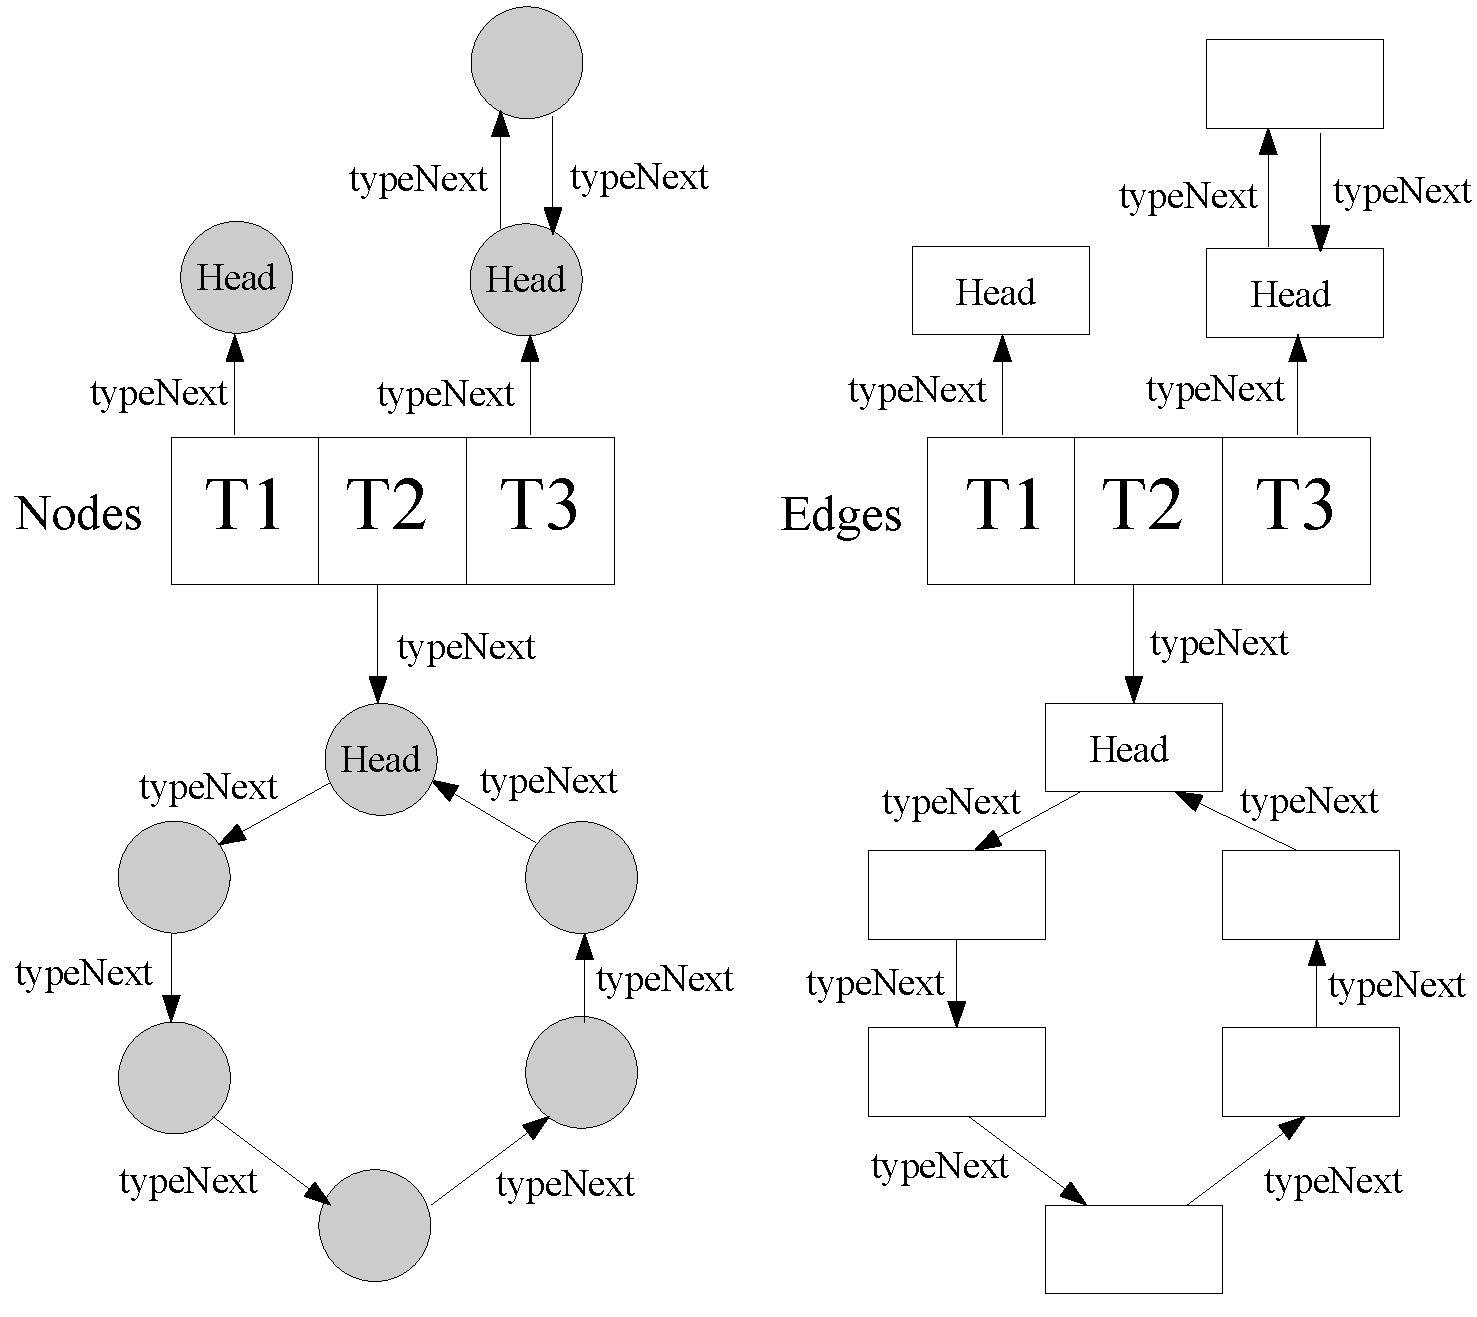
\includegraphics[width=0.65\textwidth]{fig/TypeRinglists}
  \caption{Example for type ringlists}
  \label{figtyperinglists}
\end{figure}

The connectedness information is stored in a ringlist containing the incoming edges and a ringlist containing the outgoing edges for every node object; the node object contains a field \texttt{inHead} referencing an arbitrary edge object of the incoming edges (or \texttt{null} of there is none) and a field \texttt{outHead} referencing an arbitrary edge object of the outgoing edges (or \texttt{null} if there is none).
These lists allow to quickly retrieve all incoming or all outgoing edges of a node.
The edge objects contain fields \texttt{source} and \texttt{target} referencing the source and the target node.
They give instant access to the source and target nodes of an edge.
Edges furthermore contain a field \texttt{inNext} to give the next edge in the incoming ringlist and a field \texttt{outNext} to give the next edge in the outgoing ringlist they are contained in.
All the 3 ringlists (type, in, out) are doubly linked (to allow for fast insertion and deletion), so for every \texttt{next} field there is also a \texttt{prev} field available.
The figure \ref{figincidenceexampleringlists} gives the ringlist implementation of the example graph depicted in figure \ref{figincidenceexample}. 

\begin{figure}[htbp]
  \centering
  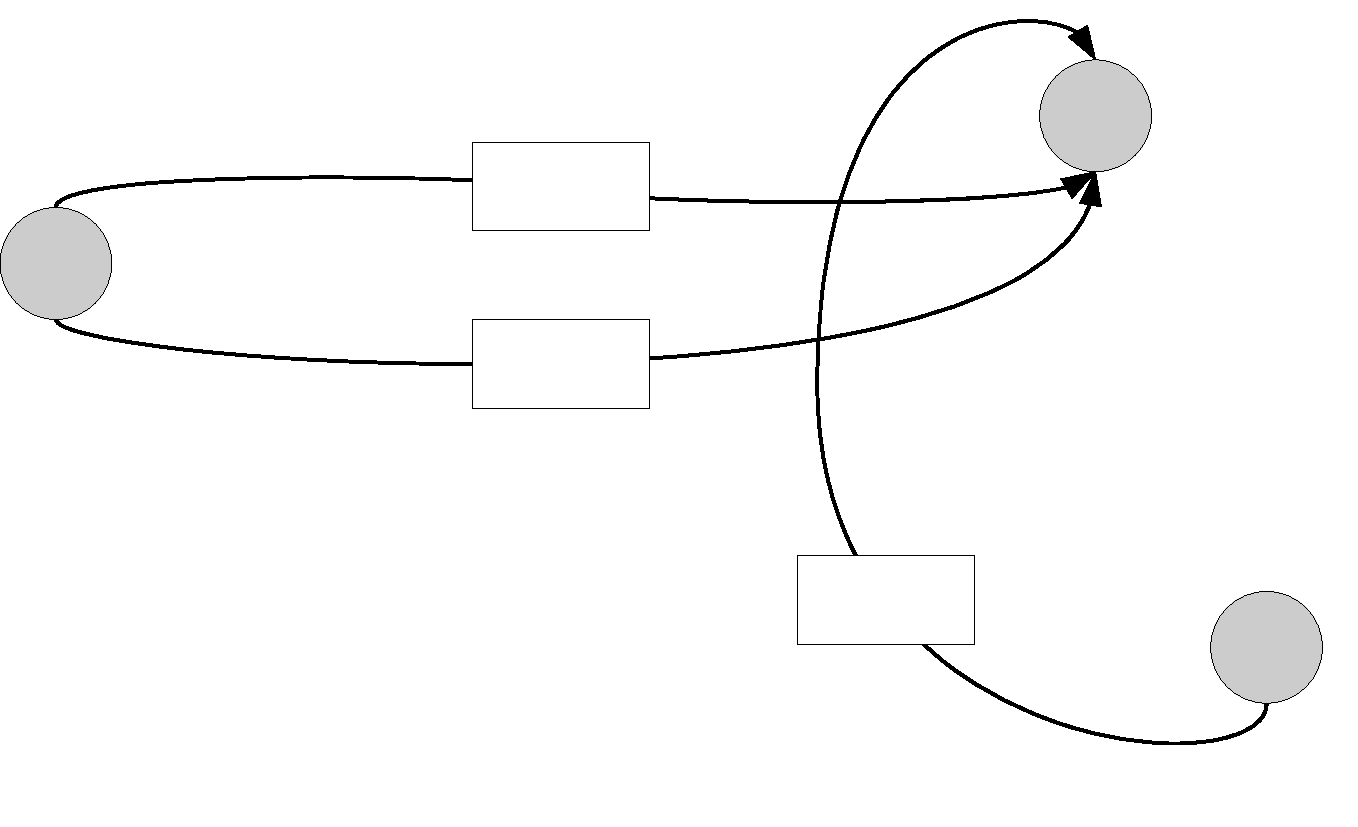
\includegraphics[width=0.75\textwidth]{fig/IncidenceExample}
  \caption{Incidence example situation}
  \label{figincidenceexample}
\end{figure}

\begin{figure}[htbp]
  \centering
  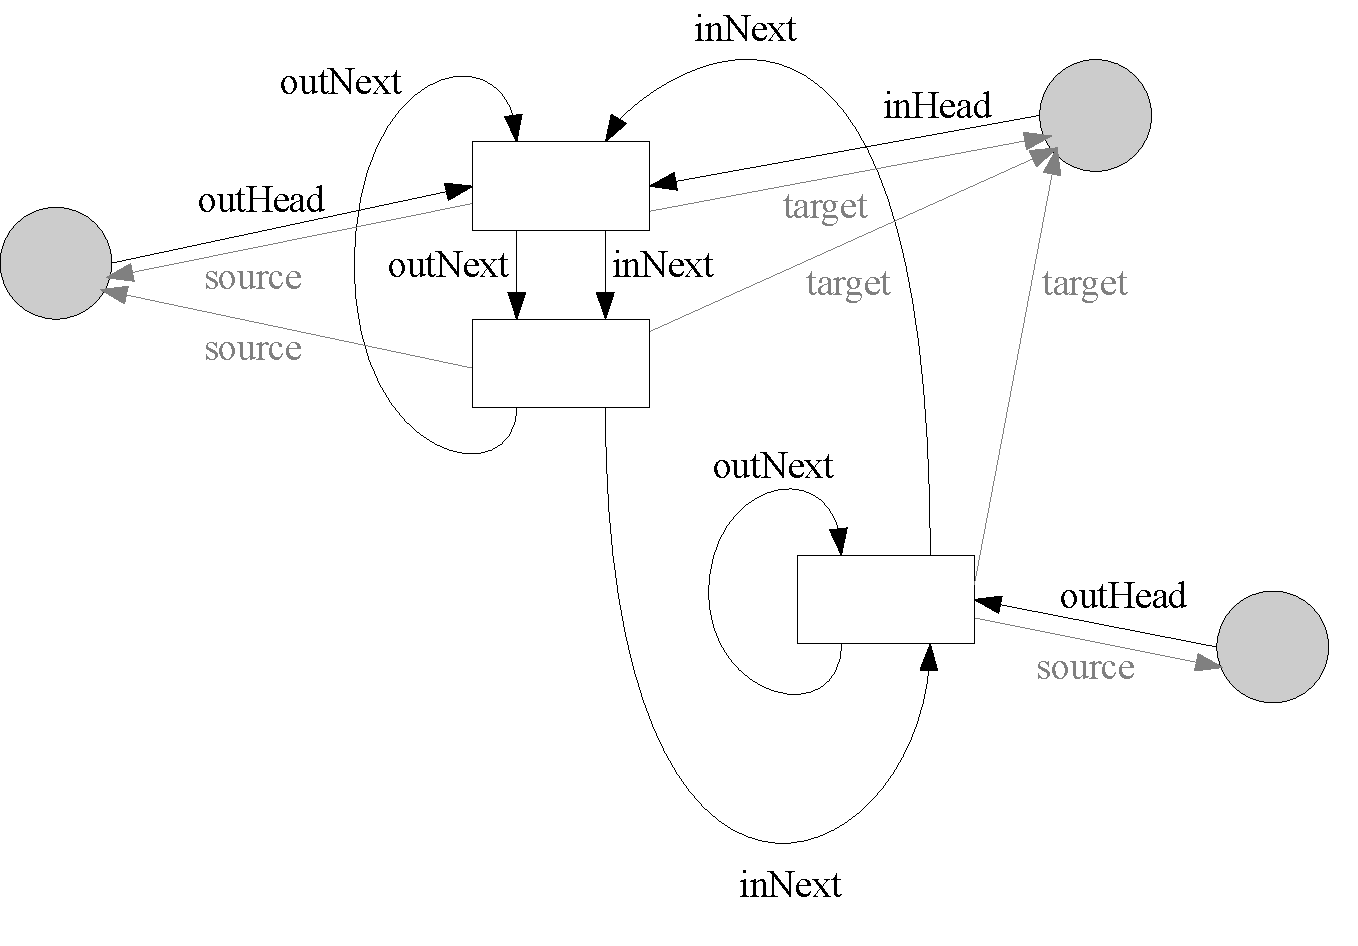
\includegraphics[width=0.75\textwidth]{fig/IncidenceExampleRinglists}
  \caption{Ringlist implementation of incidence example}
  \label{figincidenceexampleringlists}
\end{figure}


\subsection*{Pattern Matching and Search Programs}\indexmain{pattern matching implementation}\indexmain{search program}
The pattern of a rule (or test) is matched with a backtracking algorithm binding one pattern element after another to a graph element, checking if it fits to the already bound parts. If it does fit search continues trying to bind the next pattern element (or succeeds building the match object from all the elements bound if the last check succeeds), if if does not fit search continues with the next graph element; if all graph element candidates for this pattern element are exhausted, search backtracks to the previous decision point and continues there with the next element.
For every pattern to match a search program implementing this algorithm is generated, basically consisting of nested loops iterating the available graph elements for each pattern element and condition checking code continuing search with the next element to investigate.
Figure \ref{figpatterntosearchfirst} shows a pattern and a search program generated for it.

\begin{figure}[htbp]
  \centering
  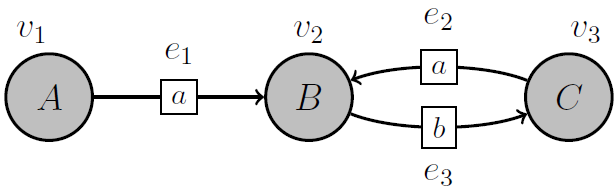
\includegraphics[width=0.7\textwidth]{fig/Pattern}
  \caption{Pattern to search}
  \label{figpatterntosearchfirst}
\end{figure}

\begin{csharp}
foreach(v1:A in graph) {
	foreach(e1 in outgoing(v1)) {
		if(type(e1)!=a) continue;
		v2 = e1.tgt;
		if(type(v2)!=B) continue;
		foreach(e3 in outgoing(v2)) {
			if(type(e3)!=b) continue;
			v3 = e3.tgt;
			if(type(v3)!=C) continue;
			foreach(e2 in outgoing(v3)) {
				if(type(e2)!=a) continue;
				if(e2.tgt!=v2) continue;
				// v1,e1,v2,e3,v3,v2 constitute a match
			} 
		}
	}
}
\end{csharp}

If a non-leaf-type (regarding inheritance hierarchy) is to be matched with a graph lookup (the outermost loop in the example), then an additional loop is used iterating all subtypes of the type of the pattern element.
If a pattern is given one or more parameters, search normally follows the graph structure by iterating the incoming or outgoing edges of a node or determining the source or target node of an edge, instead of looking up a type in the graph.
If a pattern consists of several unconnected components, several lookups are needed.
Undirected or arbitrary directed pattern edges are searched in both, the incoming and the outgoing ringlist; undirected edges are implemented by normal directed edges which can get matched in both directions.
Constraints which might cause an candidate to get rejected are the type of the element as shown in the example, structural connections to already bound elements and the isomorphy constraint.
Furthermore there are negative checking, independent checking, and attribute checking, which are normally depending on multiple elements.
Other matching operations are storage access, storage attribute access and storage mapping.

Compared to pattern matching which may need a long time, pattern rewriting is a very simple task following a simple sequence of node or edge operations, first creating all new nodes then edges, followed by an evaluation of the attributes, then deleting all edges and nodes, finally executing embedded sequences (see table \ref{table:executionorderrewriting} for more on this).

A notable performance optimization allowed by the graph model is \indexed{search state space stepping}: 
after a pattern was matched, the list heads of the type lookup ring lists, the incoming ring lists and the outgoing  ring lists are moved to the position of the matched entries with \texttt{MoveHeadAfter}, \texttt{MoveInHeadAfter} and \texttt{MoveOutHeadAfter}.
With this optimization the pattern matching during an iteration \texttt{r*} will start where the previous iteration step left of, saving the cost of iterating again through all the elements which failed in the previous iteration.

\vspace{1cm} %manual layout so the pushdown machine simulation starts on its own page

\subsection*{Pushdown Machine for Nested and Subpatterns}\indexmain{pushdown machine}\indexmain{stack machine}\label{pushdownmachine}
Every subpattern (as introduced in chapter \ref{cha:sub}) is handled with a search program corresponding to its pattern as introduced in the previous section. 
The interesting part is how the subpatterns used get combined, which happens with a $2+n$ pushdown machine.
It consists of a call stack, containing the subpattern instances found with the bound elements in the local variables of the search program frame, an open tasks stack containing the subpatterns to match (when a subpattern was matched its contained subpatterns are pushed to that open tasks stack, then the top of the stack gets processed), and $n$ result stacks containing the (partial) match object trees; for a normal rule application $n=1$, for an all-bracketed rule the number of matches is unbound.
A simulation of this machine, i.e. the matching process of a pattern using subpatterns is shown on the following pages.

Alternatives are handled like a subpattern with several possible patterns which are tried out, the first one matching is accepted.
Iterateds are handled like subpatterns whose tasks are not removed when they get matched, but only if matching failed or the maximum amount of matches was reached. In case of a failure the minimum required amount of matches is inspected, if the amount of found matches is larger or equal then matching partially succeeds and continues with the next open task (or plain succeeds if there are no open tasks left), otherwise matching of the given partial match failes causing matching to backtrack (to the previous decision point of influence).

The advantages of this design linearizing the pattern tree on the call stack are the rather low usage of heap memory, the ability to reuse the match programs for the patterns as introduced in the previous section, and the ability to find all matches (the $n$ in $2+n$ pushdown machine stands for the number of matches found).

Rewriting is carried out by a depth-first traversal of the match object tree, creating new elements before decending, evaluating attributes and deleting old elements before ascending. For each pattern piece match the modification specified in the rewrite part is carried out, i.e. the overall rewrite gets combined from the rewrites of the pattern pieces (cf. table \ref{table:executionorderrewriting} for the order of rewriting).

The subpattern usage parameters are computed during matching from matched elements and call expressions (inherited attribution), LHS yielding is carried out after the match was found during match object building within yield statements (synthesized attribution), RHS yielding is carried out during match object tree rewriting within eval statements (left attribution, with a user defined left-relation).

In the following, an example run of the $2+n$ pushdown machine is given:

\vspace{2cm} % manual layout so the pushdown simulation starts on its own page

\begin{figure}[htbp]
  \centering
  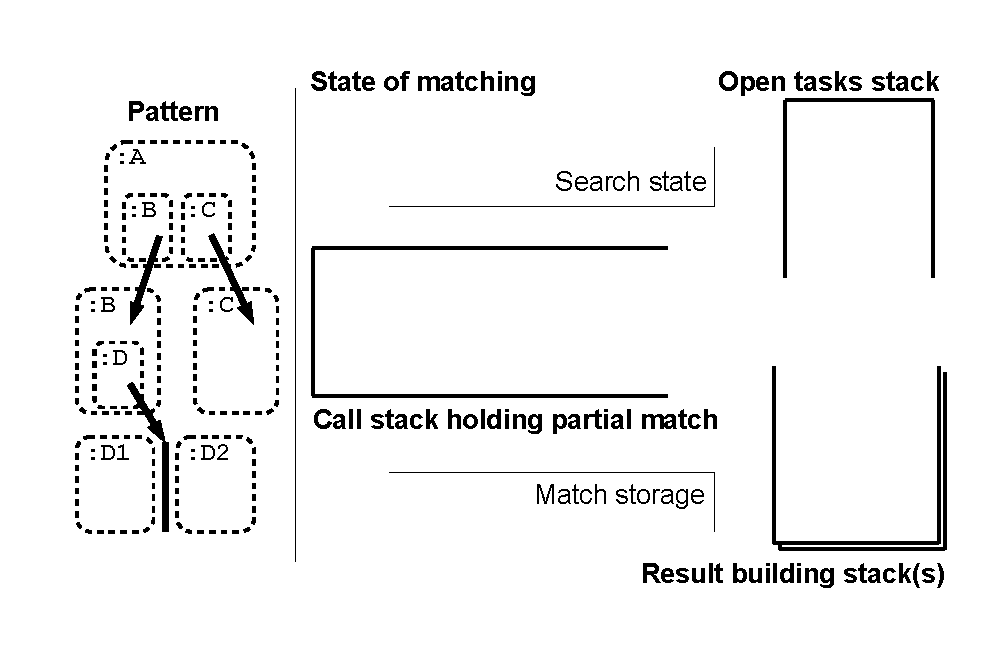
\includegraphics[width=\textwidth]{fig/Passungszustand1}
  \caption{1. Start state}
  \label{figmatchingstate1}
\end{figure}

\begin{figure}[htbp]
  \centering
  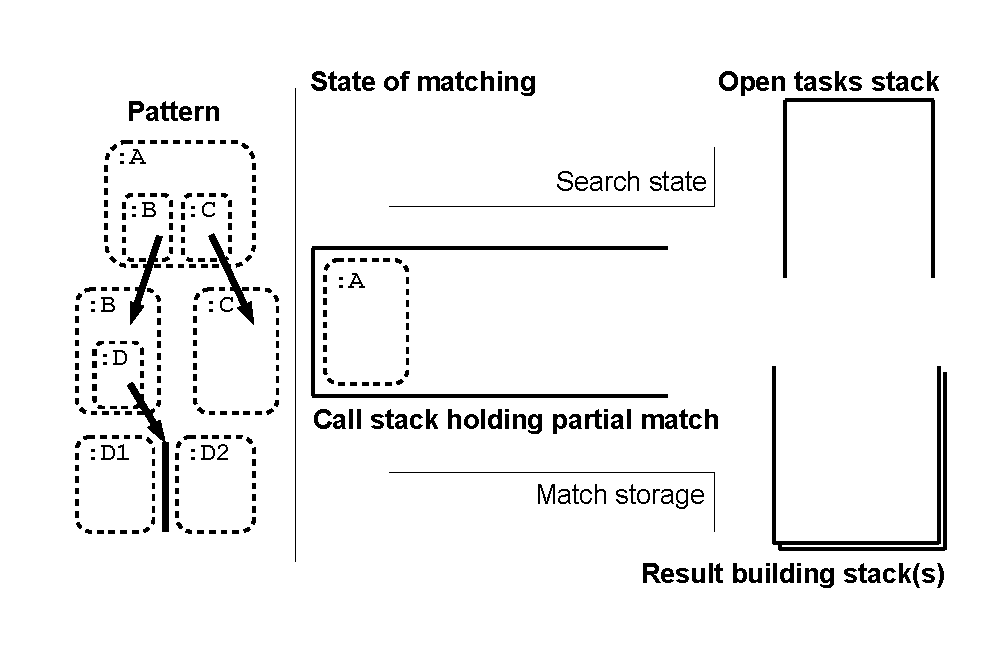
\includegraphics[width=\textwidth]{fig/Passungszustand2}
  \caption{2. The terminal part of pattern A was matched}
  \label{figmatchingstate2}
\end{figure}

\begin{figure}[htbp]
  \centering
  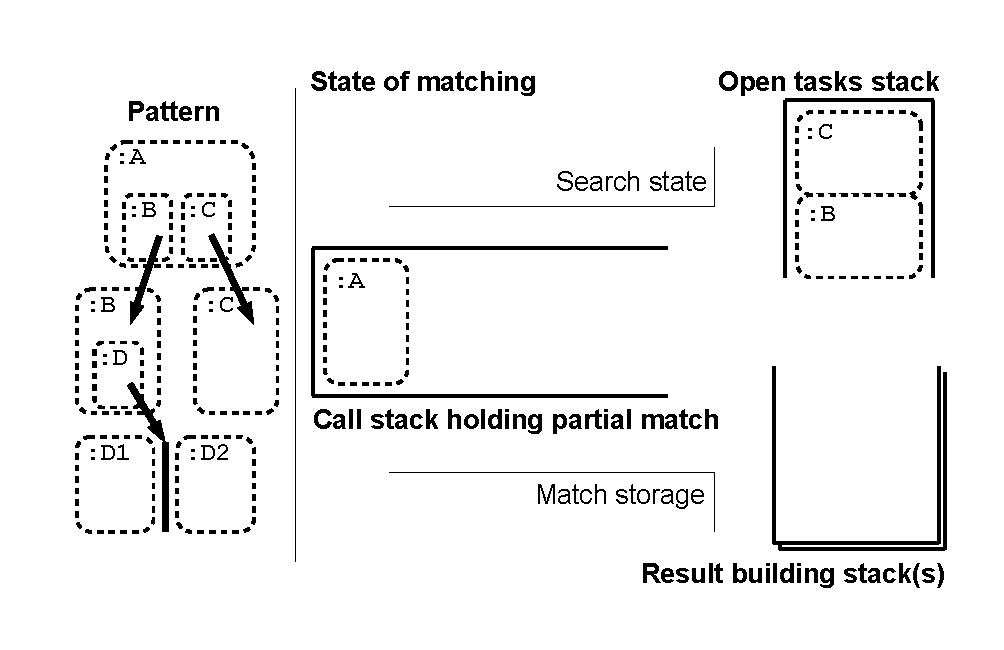
\includegraphics[width=\textwidth]{fig/Passungszustand3}
  \caption{3. The tasks for subpatterns B and C are pushed}
  \label{figmatchingstate3}
\end{figure}

\begin{figure}[htbp]
  \centering
  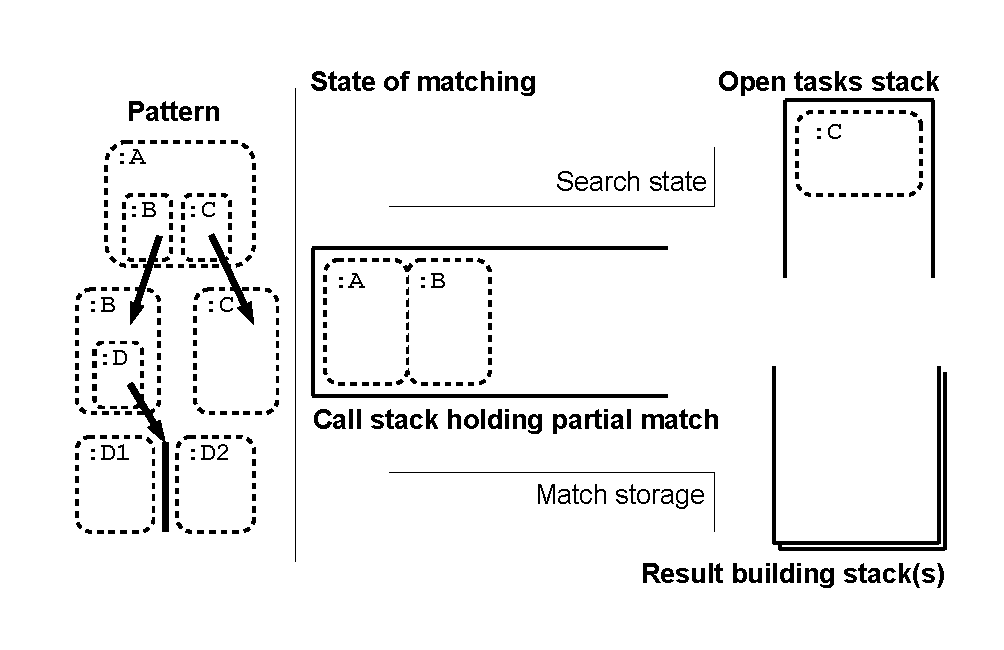
\includegraphics[width=\textwidth]{fig/Passungszustand4}
  \caption{4. The task for B gets executed, the terminal part of B was matched}
  \label{figmatchingstate4}
\end{figure}

\begin{figure}[htbp]
  \centering
  \includegraphics[width=\textwidth]{fig/Passungszustand5}
  \caption{5. The task for alternative D is pushed}
  \label{figmatchingstate5}
\end{figure}

\begin{figure}[htbp]
  \centering
  \includegraphics[width=\textwidth]{fig/Passungszustand6}
  \caption{6. The task for D gets executed, D1 is tried, but matching fails}
  \label{figmatchingstate6}
\end{figure}

\begin{figure}[htbp]
  \centering
  \includegraphics[width=\textwidth]{fig/Passungszustand7}
  \caption{7. The task for D gets executed, D2 was matched}
  \label{figmatchingstate7}
\end{figure}

\begin{figure}[htbp]
  \centering
  \includegraphics[width=\textwidth]{fig/Passungszustand8}
  \caption{8. The task for C gets executed, C was matched, a match for the overall pattern was found, but is contained only on the call stack}
  \label{figmatchingstate8}
\end{figure}

\begin{figure}[htbp]
  \centering
  \includegraphics[width=\textwidth]{fig/Passungszustand9}
  \caption{9. The match of C is popped from the call stack and pushed to the result stack}
  \label{figmatchingstate9}
\end{figure}

\begin{figure}[htbp]
  \centering
  \includegraphics[width=\textwidth]{fig/Passungszustand10}
  \caption{10. The match of D2 is popped from the call stack and pushed to the result stack}
  \label{figmatchingstate10}
\end{figure}

\begin{figure}[htbp]
  \centering
  \includegraphics[width=\textwidth]{fig/Passungszustand11}
  \caption{11. The match of B is popped from the call stack, D2 from the result stack is added, the combined match is pushed to the result stack}
  \label{figmatchingstate11}
\end{figure}

\begin{figure}[htbp]
  \centering
  \includegraphics[width=\textwidth]{fig/Passungszustand12}
  \caption{12. The match of A is popped from the call stack, B and C from the result stack are added, now we got the combined match of the overall pattern}
  \label{figmatchingstate12}
\end{figure}


% belongs logically to following section
\begin{figure}[htbp]
  \centering
  \includegraphics[width=0.7\textwidth]{fig/Pattern}
  \caption{Pattern to search}
  \label{figpatterntosearch}
\end{figure}

\begin{figure}[htbp]
  \centering
  \includegraphics[width=0.7\textwidth]{fig/Graph}
  \caption{Host graph to search in}
  \label{figgraphtosearchin}
\end{figure}


%%%%%%%%%%%%%%%%%%%%%%%%%%%%%%%%%%%%%%%%%%%%%%%%%%%%%%%%%%%%%%%%%%%%%%%%%%%%%%%%%%%%%%%%%%%%%%%%
\section{Search Planning in Code Generation}\indexmain{search plan}\indexmain{schedule}\indexmain{arborescence}\indexmain{search program}
\indexmain{host graph sensitive search plan driven graph pattern matching}\label{searchplanning}

In the previous section a search program for the pattern (repeated in figure \ref{figpatterntosearch}) was given.
It follows the schedule\\
\texttt{lkp(v1:A); out(v1,e1:a); tgt(e1,v2:B); out(v2,e3:b); tgt(e3,v3:C); out(v3,e2:a)}\\
A schedule is a more abstract version of a search program, with search operations \texttt{lkp} denoting node (or edge) lookup in the graph by iterating the type list, \texttt{out} iterating the outgoing edges of the given source node and \texttt{in} iterating the incoming edges ot the given target node, \texttt{src} fetching the source from the given edge and \texttt{tgt} fetching the target from the given edge.
For some graphs it might work well, but for the graph given in figure \ref{figgraphtosearchin} is is a bad search plan. Why so can be seen in the search order sketched in figure \ref{figbadsearch}.
Due to the multiple outgoing edges of \texttt{v1} of which only one leads to a match it has to backtrack several times. A better search order would be one matching this edge from \texttt{v2} on in reverse direction; due to the graph model containing a list of outgoing and a list of incoming edges, each edge can be traversed in either direction.

For every pattern there are normally multiple search programs available,
each able to find all the matches which exist, but with vastly different performance characteristics.
In order to improve performance, \GrG~tries to prevent following graph structures splitting into breadth as given in this example or lookups on types which are available in high quantities, by first executing a planning phase to choose a good schedule. Due to the planning phase this schedule is chosen:\\
\texttt{lkp(v3:C); out(v3,e2:a); tgt(e2,v2:B); out(v2,e3:b); in(v2,e1:a); src(e1,v1:A)}\\
corresponding to the search order depicted in figure \ref{figgoodsearch} and the search program:

\begin{csharp}
foreach(v3:C in graph) {
	foreach(e2 in outgoing(v3)) {
		if(type(e2)!=a) continue;
		v2 = e2.tgt;
		if(type(v2)!=B) continue;
		foreach(e3 in outgoing(v2)) {
			if(type(e3)!=b) continue;
			if(e3.tgt!=v3) continue;
				foreach(e1 in incoming(v2)) {
				if(type(e1)!=a) continue;
				v1 = e1.src;
				if(type(v1)!=A) continue;
				buildMatchObjectOfPatternWith(v3,e2,v2,e3,e1,v1);
			} 
		}
	}
}
\end{csharp}

\vspace{15cm}

\begin{figure}[hptb]
  \centering
  \includegraphics[width=0.7\textwidth]{fig/GraphBad}
  \caption{Bad search order}
  \label{figbadsearch}
\end{figure}

\begin{figure}[hpbt]
  \centering
  \includegraphics[width=0.7\textwidth]{fig/GraphGood}
  \caption{Good search order}
  \label{figgoodsearch}
\end{figure}

The mechanism of search planning works by computing from the pattern graph a search plan graph.
A search plan graph is an edge-weighted graph, with nodes corresponding to the pattern elements -- both nodes and edges -- and edges corresponding to operations to match them, with weight attributes giving an estimated cost of the operation. 
A search plan graph contains an additional root node, with an outgoing edge to each other node defining a \texttt{lookup} operation. From plan nodes created for nodes there are \texttt{outgoing} and \texttt{incoming} operations leaving towards plan nodes created from edges, from plan nodes created for edges there are \texttt{source} and \texttt{target} operations leaving towards plan nodes created from nodes.
The cost is determined by analyzing the amount of splitting between adjacent nodes for every triple of $(node type, edge type, node type)$ in the graph -- called a \indexed{V-Structure} -- and by counting the number of elements of every node type or edge type.
In the plan graph a minimum spanning arborescence, i.e. directed tree is computed. 
The arborescence defining the matching operations causing least cost is then linearized into a schedule, which is a list of the search operations chosen as already introduced with the good and the bad schedules.
The details of search planning and some evaluation how well it works are given in \cite{searchplangrgen} and in \cite{BKG:07}.

\begin{figure}[htbp]
  \centering
  \begin{tikzpicture}[bend angle=15]
    \tikzstyle{every node}=[minimum height=0.7cm,minimum width=0.9cm];

    \node[draw,ellipse,fill=white,inner sep=5pt] (root) at (6,0.5) {root};

    \node[draw,ellipse] (v1) at (0,5) {$\mathit{v1:A}$};
    \node[draw] (e1) at (3,5) {$e1:a$};
    \node[draw,ellipse] (v2) at (6,5) {$\mathit{v2:B}$};
    \node[draw] (e2) at (9.75,7) {$e2:a$};
    \node[draw] (e3) at (9.75,3.5) {$e3:b$};
    \node[draw,ellipse] (v3) at (13.5,5) {$\mathit{v3:C}$};

    \draw[-latex,bend left] (root.north) to node[near end, sloped, below] {$\mathsf{lkp}$/2} (v1.south);
    \draw[-latex] (root.north) -- (e1.south) node[near end, sloped, below] {$\mathsf{lkp}$/7};
    \draw[-latex] (root.north) -- (v2.south) node[midway, sloped, below] {$\mathsf{lkp}$/4};
    \draw[-latex,bend right] (root.north) to node[near end, sloped, below] {$\mathsf{lkp}$/7} (e2.south);
    \draw[-latex] (root.north) -- (e3.south) node[near end, sloped, below] {$\mathsf{lkp}$/2};
    \draw[-latex,bend right,line width = 2pt] (root.north) to node[near end, sloped, below] {$\mathsf{lkp}$/1} (v3.south);

    \draw[-latex,bend left] (v1) to node[midway, above] {$\mathsf{out}$/2.83} (e1);
    \draw[-latex,bend left,line width = 2pt] (e1) to node[midway, below] {$\mathsf{src}$/1} (v1);
    \draw[-latex,bend right] (e1) to node[midway, below] {$\mathsf{tgt}$/1} (v2);
    \draw[-latex,bend right,line width = 2pt] (v2) to node[midway, above] {$\mathsf{in}$/1} (e1);
    \draw[-latex,bend left] (v2) to node[midway, above] {$\mathsf{out}$/1} (e2);
    \draw[-latex,bend left,line width = 2pt] (e2) to node[midway, below] {$\mathsf{src}$/1} (v2);
    \draw[-latex,bend left,line width = 2pt] (v2) to node[midway, above] {$\mathsf{out}$/1} (e3);
    \draw[-latex,bend left] (e3) to node[midway, below] {$\mathsf{src}$/1} (v2);
    \draw[-latex,bend right] (e2) to node[midway, below] {$\mathsf{tgt}$/1} (v3);
    \draw[-latex,bend right,line width = 2pt] (v3) to node[midway, above] {$\mathsf{in}$/1} (e2);
    \draw[-latex,bend right] (e3) to node[midway, below] {$\mathsf{tgt}$/1} (v3);
    \draw[-latex,bend right] (v3) to node[midway, above] {$\mathsf{in}$/2} (e3);
  \end{tikzpicture}
  \caption{
  	The search plan graph for the pattern graph of Figure~\ref{figpatterntosearch} with estimated backtracking costs induced by the host graph of Figure~\ref{figgraphtosearchin}.
	The found minimum directed spanning tree is denoted by thick edges.
  }
  \label{fig:plan-graph}
\end{figure}


A search program is a lower abstraction version of a schedule.
Structurally it is a tree data structure reflecting the syntax tree of the code to generate (with list entries maybe containing further lists), as sketched in figure \ref{figsearchprogram}; in contrast to the schedule which is a simple list data structure.

\begin{figure}[htbp]
  \centering
  \includegraphics[width=0.9\textwidth]{fig/SearchProgram}
  \caption{A simple Search Program}
  \label{figsearchprogram}
\end{figure}

It contains explicit instructions for isomorphy checking and connectedness checking, which are inserted after the schedule was determined along the exact sequence of instructions.
Connectedness checking can be seen in the good search program of the example in the check that the target of \texttt{e3} is indeed \texttt{v3};
a target matching operation \texttt{tgt(e3,v3:C)} is not used because \texttt{v3} was already matched by the lookup operation, and is already contained in the spanning tree.
Furthermore it contains exact locations where to continue at, which might be different than the directly preceding search operation (because that one does not define a choice point of influence).

A remark on isomorphy handling: As a consequence of the simple loop based graph element binding to pattern elements, without an explicit check all pattern elements could get matched completely homomorphically to each other (due to the loops starting with the same elements, the homomorphic matches \emph{are} normally the first to be found).
To ensure that two pattern elements are not bound to the same graph element, flags contained in the graph elments are set when a graph element is bound to a pattern variable and reset when the binding is given up again (one flag for each negative/independent nesting level, until the implementation defined limit of flags available in the graph elements is reached, then a list of dictionaries is used); the flags are checked then in the following, nested matching operations. An iso-check scheduling pass ensures that checks are only inserted if the elements must be isomorphic and their types do not already ensure that they can't get matched to the same elements.


%%%%%%%%%%%%%%%%%%%%%%%%%%%%%%%%%%%%%%%%%%%%%%%%%%%%%%%%%%%%%%%%%%%%%%%%%%%%%%%%%%%%%%%%%%%%%%%%
\section{The Code Generator}\indexmain{code generator}

\subsection{Frontend}

\begin{figure}[htbp]
  \centering
  \includegraphics[width=\textwidth]{fig/AblaufCodeerzeugungFrontend}
  \caption{Frontend Code Generation}
  \label{figfrontendcodegen}
\end{figure}

The frontend is spread over the directories \texttt{parser}, \texttt{ast}, \texttt{ir}, \texttt{be} and \texttt{util}, with their code being used from \texttt{Main.java}.

\subsubsection*{Syntax and Static Semantics}
The directory \texttt{parser} contains parser helpers like the symbol table and scopes and within the \texttt{antlr} subdirectory the ANTLR parser grammar of \GrG~in the file \texttt{Grgen.g}.
The semantic actions of the parser build an abstract syntax tree consisting of instances of the classes given in the directory \texttt{ast}, with the base class \texttt{BaseNode}.
The AST is operated upon in three passes, first resolving by \texttt{resolve} and \texttt{resolveLocal}, mainly replacing identifier nodes by their declaration nodes during a (largely) preorder walk.
Afterwards the AST is checked by \texttt{check} and \texttt{checkLocal} during a (largely) postorder walk for type and other semantic constraints.
Finally an intermediate representation is built from the abstract syntax tree by the \texttt{getIR} and \texttt{constructIR} methods.

\subsubsection*{Intermediate Representation}
The IR classes given in the \texttt{ir} folder can be seen as more lightweight AST classes; their name is often the same as for their corresponding AST classes, but without the \texttt{Node}-suffix which is appended to all AST classes.
The most interesting classes are \texttt{Rule} used for rules, alternative cases and iterateds, as well as \texttt{PatternGraph} used for all pattern graphs including negatives and independents;
several data flow analyses are contained in \texttt{PatternGraph}, some covering the nesting of patterns, some being even global.
A particularily interesting one is \texttt{ensure\-Directly\-Nesting\-Pattern\-Contains\-All\-Non\-Local\-Elements\-Of\-Nested\-Pattern} which ensures that, from a pattern which contains a certain entity the first time, up to every pattern that references this entity, all intermediate patterns contain that entity, too.

This is done in a recursive walk over the nested patterns in the IR-structure. 
Each pattern receives the set of already known elements as parameter,
before descending the elements available in the current pattern are added to the set of already known elements,
then recursive descent into the directly nested patterns follows handing down the already known elements.
On ascending elements are added to the current pattern if they are contained in a directly nested pattern, but not in the current pattern, although they are known in the current pattern.

This is done in the IR to keep the backends simple.
The IR classes are the input to the two backends of the frontend, as given in the folders \texttt{be/C} and \texttt{be/Csharp}.


\subsubsection*{Backends}

The directory \texttt{be/C} contains the code generator for the C based backend integrated into the IPD C compiler.
(The compiler transforms a C program into a graph and SSA based compiler intermediate representation named FIRM using libFirm (see \url{libfirm.org}, \cite{TBL:99}, \cite{Lin:02}) and further on to x86 machine code.)

The directory \texttt{be/Csharp} contains the code generator for the C\# based backend of \GrG. 
It generates the model source code \texttt{FooModel.cs} with the node and edge classes for a rule file named \texttt{Foo.grg}, 
and the intermediate rules source code \texttt{FooActions\_intermediate} with a description of the patterns to match, a description of the embedded graph rewrite sequences, and the rewriting code.
This is done in several recursive passes over the nesting structure of the patterns in the IR. 

The backend of the frontend does \emph{not} generate the complete rules source code with the matcher code or the code for the embedded rewrite sequences --- this is done by \texttt{grgen.exe} which only calls the \texttt{grgen.jar} of the frontend.
You may call the Java archive on your own to get a visualization of the model and rewrite rules from a \texttt{.vcg}-dump of the IR, cf. Note\ref{note:modelruledump}.


\subsubsection*{Model Generation}

The model generation code in \texttt{ModelGen} is rather straight forward:
\begin{enumerate}
	\item first code for the user defined enums is generated,
	\item then the node classes are generated,
	\item followed by the node model,
	\item then the the edge classes are generated,
	\item followed by the edge model,
	\item and finally the graph model is generated.
\end{enumerate}

\noindent For the nodes as well as for the edges three classes are generated:
\begin{enumerate}
	\item the first being the interface visible to the user, giving access to the attributes,
	\item the second being the implementation implementing the interface and inheriting from \texttt{LGSPNode} or \texttt{LGSPEdge},
	\item and the third being a type representation class inheriting from \texttt{NodeType} or \texttt{EdgeType} giving informations about the type and its attributes, used in the node/edge model and thus graph model.
\end{enumerate}


\subsubsection*{Rule Representation Pass}

The action code, better representation generation is implemented in \texttt{ActionsGen}, in the code called from \texttt{gen\-Subpattern} for the subpatterns and \texttt{gen\-Action} for the rules and tests on.

In a prerun from \texttt{gen\-Rule\-Or\-Subpattern\-Class\-Entities} on some needed entities are generated, e.g. type arrays for the allowed types of the pattern elements (the arrays are only filled if the base type was constrained), or indexing enums, which map the pattern element names to their index in the arrays of the matched host graph elements in the match objects of the generic match interface.

In the rule representation pass from \texttt{gen\-Rule\-Or\-Subpattern\-Init} on the subpattern- and rule representations of type \texttt{Matching\-Pattern} and \texttt{Rule\-Pattern} are generated, including the contained \texttt{Pattern\-Graph}-objects for the (nested) pattern graph(s), in a mutual recursion game of \texttt{gen\-Pattern\-Graph} and \texttt{gen\-Elements\-Required\-By\-Pattern\-Graph}.

The method \texttt{gen\-Elements\-Required\-By\-Pattern\-Graph} generates for a pattern graph its contained elements, the pattern nodes, the pattern edges, the used subpatterns as \texttt{Pattern\-Graph\-Embedding} members, the contained alternatives, and the iterateds; the representations of contained negative subpatterns and alternative cases get generated via \texttt{gen\-Pattern\-Graph} before the containing pattern. 

A graph element contained in pattern, but defined in a nesting pattern, is saved in the pattern as a reference to the element in the nesting pattern. 
The \texttt{Pattern\-Graph} in which it was used first is remembered in a \texttt{Point\-Of\-Definition}-membervariable.
The source and target nodes of edges are saved in the \texttt{Pattern\-Graph} in hash tables (so that an edge with an undefined target can receive a target in a nested pattern), source and target nodes are determined by ascending along the pattern nesting until a definition is found.

As all graph elements, including the ones of the nested patterns, are created flatly in the \texttt{initialize}-method of the \texttt{Matching\-Pattern}, name prefixes are needed to prevent name clashes; this is ensured by the parameter \texttt{path\-Prefix}.
Correct naming of already declared elements is ensured with a \texttt{already\-Defined\-Entity\-To\-Name}-hash-table.
The split into constructor and \texttt{initialize}-Methode ist needed because a recursive \texttt{Matching\-Pattern} must reference itself at construction.

Furthermore expressions trees for the attribute checks are generated, as well as local and global homomorphy tables for the nodes and the edges, defining which pattern elements may match the same host graph element (the global tables specify the homomorphy in between elements from the \texttt{Pattern\-Graph} of an alternative case or an iterated and an enclosing \texttt{Pattern\-Graph}).


\subsubsection*{Rewrite Code Pass}
In the rewrite pass the rewrite code gets generated, via \texttt{gen\-Modify} of \texttt{Modify\-Gen};
the nesting of negative or independent patterns does not need to be taken care of here as they don't possess rewrite parts.

For every pattern piece and its replacement role (dependent rewriting, creation, deletion) are local rewrite methods generated, bringing at runtime the overall rewriting into effect by calling each other.
\texttt{Modify\-Generation\-State} holds the state during generation, while the \texttt{Modify\-Generation\-Task}s allow to give a left and right graph independent of the rewriting specified with the rule. The code for subpattern creation is generated by using an empty graph as left graph and the pattern graph as right graph, the code for subpattern deletion is generated by using the pattern graph as left graph and an empty graph as right graph, for a dependent rewrite the graphs from \texttt{IR::Rule} are simply referenced, for a test the pattern graph is used as left and right graph.
For alternatives and iterateds dispatching methods get generated calling the rewrite methods of the instances of the patterns matched.
Rewrite parameters are mapped to local parameters of the rewrite methods.

The core method of rewrite code generation \texttt{gen\-Modify\-Rule\-Or-Subrule} generates the rewriting of the given pattern and the calls to the rewrite methods of the nested patterns.
Because the rewrite methods of the nested patterns are placed flatly in their \texttt{Matching\-Pattern} or \texttt{Rule\-Pattern}, they receive their nesting path as name prefix, their role is distinguished by one of the name postfixs \texttt{Modify}, \texttt{Create} or \texttt{Delete}; for keeping a pattern unmodified obviously no methods are needed.

For embedded sequences \texttt{LGSPEmbeddedSequenceInfo} objects are generated, which do contain the sequence as string plus additional parameter informations, the real sequence code is generated in the backend.
For sequences embedded in alternatives, iterateds, or subpatterns additionally closure classes inheriting from \texttt{LGSPEmbeddedSequenceClosure} are generated.
They store the graph elements the pattern elements were bound to of the pattern containing the exec; the sequence execution function is then called from this closure, which is stored in a queue and executed from the top level rule.

Finally match classes are generated, for every pattern besides negative patterns an interface and a class implementing this interface.
The match classes are instantiated after a match of the corresponding pattern was found, giving a highly convenient and type safe interface to the matched entities to the user at API level.


\subsection{Backend}

The real matcher code is generated by the backend given in \texttt{engine-net-2}, in the \texttt{src/lgspBackend} subdirectory.
The processing is done in several passes in \texttt{lgsp\-Matcher\-Generator.cs}; the base data structure is the \texttt{PatternGraph}, resp. the nesting of the \texttt{PatternGraph}-objects, contained in the \texttt{RulePattern}-objects of the rules/tests or the \texttt{Matching\-Pattern}-objects of the subpatterns.

\pagebreak

\subsubsection*{1. Step}

\begin{figure}[htbp]
  \centering
  \includegraphics[width=\textwidth]{fig/AblaufCodeerzeugungBackend1}
  \caption{Backend Code Generation, step 1}
  \label{figbackendcodegen1}
\end{figure}

First the subpattern usages are inlined when \indexed{inlining} is assumed to be benefitial; this allows the programmer to extract common patterns into subpatterns increasing readability and modularity without loosing performance (but as of now only one level of inlining is supported, so beware of too much subpattern extraction, especially if the containing pattern would get disconnected by this). 
After (and partly before) this pattern rewriting the patterns and their relations are analyzed by the \texttt{PatternGraphAnalyzer} -- the analyze results are used for emitting better code later on (choosing more efficient but more limited implementations for language features which are not sufficient in the general case but are so for the specification at hand).
Then a \texttt{PlanGraph} is created from the \texttt{PatternGraph} and data from analyzing the host graph (for generating the initial matcher some default data given from the frontend is used).
A mimimum spanning arborescence is computed defining a hopefully optimal set of operations for matching the pattern (the hopes are founded, see \cite{BKG:07}).
A \texttt{SearchPlanGraph} is built from the arborescence marked in the \texttt{PlanGraph} and used thereafter for scheduling the operations into a \texttt{ScheduledSearchPlan}, which gets completed by \texttt{Append\-Homomorphy\-Information} with isomorphy checking information.
The \texttt{ScheduledSearchPlan} is then stored in the \texttt{PatternGraph} it was computed from.


\subsubsection*{2. Step}

\begin{figure}[htbp]
  \centering
  \includegraphics[width=0.5\textwidth]{fig/AblaufCodeerzeugungBackend2}
  \caption{Backend Code Generation, step 2}
  \label{figbackendcodegen2}
\end{figure}

In a second step the \texttt{Schedules} of the negative or independent \texttt{Pattern\-Graph}s are integrated into the \texttt{Schedule} of the enclosing \texttt{Pattern\-Graph}, by \texttt{Merge\-Negative\-And\-Independent\-Schedules\-Into\-Enclosing\-Schedules} in a recursive run over the nesting structure of the \texttt{Pattern\-Graph}s in the \texttt{Matching\-Pattern}s or \texttt{Rule\-Pattern}s.
Due to nested negative or independent graphs this may happen spanning several nesting levels;
the result is saved in the \texttt{Schedule\-Including\-Negatives\-And\-Independents} field of the non-negative/independent \texttt{Pattern\-Graph}s.


\subsubsection*{3. Step}

\begin{figure}[htbp]
  \centering
  \includegraphics[width=\textwidth]{fig/AblaufCodeerzeugungBackend3}
  \caption{Backend Code Generation, step 3}
  \label{figbackendcodegen3}
\end{figure}

Finally, in a third step code is generated by \texttt{Generate\-Matcher\-Source\-Code},
again in a recursive run over the nesting structure of the \texttt{Pattern\-Graph}s, 
using the \texttt{Schedule\-Including\-Negatives\-And\-Independents} stored in them. 

For each \texttt{Rule\-Pattern} an \texttt{Action}-class is generated, 
and for each \texttt{Matching\-Pattern} a \texttt{Subpattern\-Action}-class is generated.
Additionally for each alternative or iterated which is nested in a rule, test, or subpattern,
an \texttt{Alternative\-Action}-class or an \texttt{Iterated\-Action}-class are generated;
the alternative matcher will contain code for all alternative cases.
The real matching code is then generated into these classes.

The \texttt{SearchProgramBuilder} builds a \texttt{SearchProgram} tree data structure resembling the syntax tree of the code to generate out of the \texttt{Schedule\-Including\-Negatives\-And\-Independents} in the \texttt{Pattern\-Graph}s. 
In a further pass the \texttt{SearchProgram} is completed by the \texttt{Search\-Program\-Completer},
determining the locations to continue at when a check fails,
writing undo code for the effects which were applied from that point on to the current one.
Finally the C\# code gets generated by calling the \texttt{Emit} methods of the \texttt{SearchProgram}.
If you want to extends this code you may be interested in the \texttt{Dump} methods which dump the \texttt{SearchProgram} in an easier readable form into text files.

The \texttt{Subpattern\-Action}-classes do not only contain the matcher code, 
but are at the same time the tasks of the $2+n$ pushdown machine, which are pushed on the open tasks stack;
they contain the subpattern parameters as member variables.
The same holds for the \texttt{Alternative\-Action}- and \texttt{Iterated\-Action}-classes,
which do not hold parameters but entities from the nesting pattern they reference. 


\subsubsection*{Nested and Subpattern Matching}

The higher levels of code generation are in large parts independent from nested and subpattern matching and control of the $2+n$ pushdown machine.
Only on the level of search programs it becomes visible,  
with an \texttt{Initialize\-Subpattern\-Matching}-search program operation at the begin of a search program
and a \texttt{Finalize\-Subpattern\-Matching}-search program operation at the end of a search program;
but mainly with a call to \texttt{build\-Match\-Complete} when the end of the schedule is reached during search program builing.
This corresponds to the innermost location in the search program,
the location at which during execution the local pattern was just found;
now the control code is inserted by \texttt{insert\-Push\-Subpattern\-Tasks},
pushing the tasks for the subpatterns used from this pattern, as well as alternatives and iterateds nested in this pattern.
To execute the open tasks a \texttt{Match\-Subpatterns} operation is inserted into the search program. 
Afterwards \texttt{insert\-Pop\-Subpattern\-Tasks} inserts the operations for cleaning the task stack,
\texttt{insert\-Check\-For\-Subpatterns\-Found} the operations to handle success and failure, 
and \texttt{insert\-Match\-Object\-Building} the code for maintaining the result stack.


\subsubsection*{Further Functionality}

The compiled graph rewrite sequences are handled by the \texttt{lgsp\-Sequence\-Checker} and \texttt{lgsp\-Sequence\-Generator} (together with the sequence parser from the libGr).
The \texttt{src/GrGen} subdirectory contains the \texttt{grgen.exe} compiler driver procedure.
The \texttt{src/libGr} subdirectory contains the libGr, offering the base interfaces a user of \GrG~sees on the API level for the model, the actions, the pattern graphs and the host graph.
The interfaces get implemented by code from the libGr search plan (lgsp) backend and by the generated code.
The libGr further offers a generic, name string and object based interface to access the named entities of the generated code.
In addition it offers the rewrite sequence parser which gets generated out of \texttt{SequenceParser.csc},
building the rewrite sequence AST from the classes in \texttt{Sequence.cs} further utilizing \texttt{SymbolTable.cs}.
The rewrite sequence classes contain a method \texttt{ApplyImpl(IGraph graph)} which executes them.
Finally the libGr offers several importers and exporters in the \texttt{src/libGr/IO} subfolder.

When GrGen rules are matched in the graph and when the graph is changed by rule rewriting then events are fired.
They allow to to display the matches and changes to the user in the debugger,
to record changes to a file for later playback, or record changes to a transaction undo log for later rollback, 
or to execute user code if event handlers are registered to them,
allowing users to build an event based graph rewriting mechanism on API level.
The graph delegates fired are given in \texttt{IGraph.cs}.
Graph events recording is implemented in \texttt{Recorder.cs} (replaying is normal \texttt{.grs} execution);
graph transaction handling is implemented in \texttt{lgspTransactionManager.cs}, with a list of undo items which know how to undo the effect on the graph which created them, which are purged on commit or executed on rollback.
Backtracking is implemented with nested transactions.
If you are changing the graph programmatically not using GrGen rules you have to fire the events on your own in case you want to use any of the mechanisms (graphical debugging, record and replay, transactions and backtracking, event based programming) above.

The \texttt{src/GrShell} subdirectory contains the GrShell application, which builds upon the generic interface (as it must be capable of coping with arbitrary used defined models and actions at runtime) and the sequence interpretation facilities offered by the libGr.
The command line parser of GrShell gets generated out of \texttt{GrShell.csc}, the shell implementation is given in \texttt{GrShellImpl.cs}.
Graphical debugging is offered by the \texttt{Debugger.cs} together with the \texttt{YCompClient.cs}, which implements the protocol available for controling yComp, communicating with yComp over a tcp connection to localhost.

The \texttt{examples} subdirectory of \texttt{engine-net-2} contains a bunch of examples for using \GrG~with GrShell.
The \texttt{examples-api} subdirectory contains several examples of how to use \GrG~from the API.
In case you want to contribute and got further questions don't hesitate to contact us 
(via email to \texttt{grgen} at the host given by \texttt{ipd.info.uni-karlsruhe.de}).


%%%%%%%%%%%%%%%%%%%%%%%%%%%%%%%%%%%%%%%%%%%%%%%%%%%%%%%%%%%%%%%%%%%%%%%%%%%%%%%%%%%%%%%%%%%%%%%%
\section{Performance Optimization}\label{sec:performance} \indexmain{performance}\indexmain{optimization}

The most important point to understand when optimizing for speed is that the expensive task is the search carried out during pattern matching. The effort for rewriting, the dominant theme in graph rewriting literature, is negligible.

\subsubsection*{Use Types}
A corollary from what you've seen especially in section \ref{searchplanning} is: \emph{Use types!}\\
The more fine grain a graph is typed, the better are the statistics regarding the splitting structures (V-Structures) and the number of elements of a certain type, yielding better search plans evading splitting structures and employing least-cost lookups, pruning non-matches earlier in the search.
Even if only the initial static schedules are used which do not know about the splitting factors or the type weights, fine grain types cause a quicker search pruning with the type checks.
You may improve the static schedules by explicitely giving search priorities.
Using fine-grain types is easy in GrGen, for multiple inheritance on node and edge types (cf. \ref{nodeandedgetypes}) is supported.

\begin{warning}
Search planning is only carried out on request!
You must analyze the graph and then re-generate the matchers at runtime,
with \texttt{custom graph analyze} and \texttt{custom actions gen\_searchplans} (issued on the command line or to the \texttt{Custom} methods of the graph and the actions objects);
you may have a look at the effects of replanning with the \texttt{custom actions explain <actionname>} command.
See subsection \ref{custom} for more on this.
\end{warning}

\subsubsection*{Memorize, Don't Search}
Often in a transformation you know the location you want to process from a previous step.
In this case, store these locations in variables of node (or edge) type, and hand them in as parameters to the rules and return them out from the rules.
In case of a statically not known number of locations as they appear e.g. in wavefront algorithm, you may store the locations in storages (cf. chapter \ref{cha:container}), i.e. collection valued variables (which are iterated over in the sequences or passed to the rules as \texttt{ref} parameters).
Search will then start from these parameters, instead of a looking up a value in the graph by type (unless search planning taking the statistics about the graph into account comes to the conclusion  that a lookup on a very seldom type is still the better approach).

A sophisticated way of remembering facts about non-local properties is to computed them with data flow analyses (see section \ref{subsub:flow}) and store them as attributes in the graph elements.
This allows to replace searching for distant values, or global properties like reachability, by checking a local property, at the price of re-running an analysis every time the graph changes in an important way.

Speaking in database parlance, with storages you can build indices into the graph, indices which are more selective than the automatically built indices by graph element type; but in contrast to the automatically built ones, you must maintain them by hand.

The approach of remembering state instead of searching when needed has a clear caveat: the code becomes less readable and more brittle. As in normal programming, you must balance performance optimizations against maintainability.

\subsubsection*{Use Compiled Sequences}
The compiled sequences given in the rules file are executed a good deal faster than the interpreted sequences given in the shell.
So if you need speed, replace interpreted sequences by compiled ones.
The price you pay is a loss of debuggability, a compiled sequence can only be executed as one big step.

\subsubsection*{Beware of Disconnected Patterns}
Subpatterns are searched top-down (cf. \ref{pushdownmachine}), from the input parameters on.
If the input arguments are disconnected in the pattern containing the subpattern, the containing pattern enumerates the cross product of the matches of the disconnected parts, which is then later on filtered in the subpattern called for the ones which are connected.
This will likely wreak havoc on the search performance.
It might be more efficient to just search from a start parameter a connected end location, and yield the found one out (cf. \ref{sec:localvarorderedevalyield}), or to search from a start parameter all connected end locations, collecting the found ones in a result set; and to check the ones found alongside connectedness in a second step.

The same holds for the nested patterns, just that parameter passing is implicit there, the elements from the containing pattern which are referenced in the nested pattern are passed in automatically as arguments.
The holds especially for the \texttt{alternative} and \texttt{iterated} constructs which are matched with the pushdown machine (cf. \ref{pushdownmachine}), too, but also for the \texttt{negative} and \texttt{independent} constructs which are matched with nested local code embedded into the matcher code of their containing pattern.

Just as a side remark: the performance issue is raised by the local disconnected pattern and the caused multiplication of the part matches.
This combinatorial explosions appears even within a single local pattern, only that it is more obvious there what is going on compared to the case that you disconnected a pattern later on by factoring out a common part into a subpattern.
Luckily in this situation a performance hit is unlikely due to the subpattern \indexed{inlining} supported by GrGen; which in addition to connecting disconnected patterns removes the pushdown machine overhead.

But take into account that the \emph{subpattern inlining} implemented in GrGen is limited to depth one.
If a pattern is disconnected over two or more levels of subpattern usage (which might happen statically with one subpattern using another subpattern, and will for sure dynamically on a subpattern recursion path), it will hit performance.
You may have a look at the output of the \texttt{explain} command (cf. \ref{custom}) to see  if the subpatterns are disconnected; this is indicated by multiple lookups in the containing pattern, and the fact that the starting points passed as preset parameters to the nested or subpatterns get connected only there with search commands.

\subsubsection*{Miscellaneous Things}
\begin{itemize}
  \item Visited flags are the most efficient way of marking elements, if a large number of the elements gets marked. Otherwise they are inefficient, cause a lot of elements need to be iterated, just to filter the visited ones out. Storages which give quick access to their contained elements are better then. Or even reflexive marker edges of a special type in the graph.
	\item Prefer all-bracketing (cf. \ref{sec:ruleapplication}) over iteration for rule application. This is only possible if the parts of the matches which are to be modified, e.g. retyped, are disjoint.
\end{itemize}


\appendix

\bibliographystyle{alpha}
\bibliography{diss}

\printindex

\end{document}



